\documentclass[a4paper,oneside,14pt]{scrbook}


\usepackage[utf8]{inputenc}
\usepackage{amsmath}
\usepackage{amsfonts}
\usepackage{amsthm}
\usepackage[russian]{babel}
\usepackage{indentfirst}
\usepackage[colorlinks=true]{hyperref}
\usepackage{graphicx}
\usepackage[all]{xy}
\usepackage{algorithm}
\usepackage{algorithmic}
\usepackage{ifthen}

%пометка черновика (закомментировать три строки ниже для релиза)
\usepackage{draftwatermark}
\SetWatermarkScale{1.5}
\SetWatermarkText{$\beta$-версия от \today}


\title{Учебное пособие по дисциплине\\<<Дискретная математика>>}
\author{\fbox{Т.~Р.~Фадеева}, М.~М.~Шихов}
\date{\today}

\newtheorem{exampl}{Пример}[chapter]
\newtheorem{Theor}{Теорема}[chapter]

%для рисования графов пакетом xy-pic
\entrymodifiers={++[o][F-]}

%для псевдокода алгоритмов (algorithm,algorithmic)
\renewcommand{\algorithmicrequire}{\textbf{Вход:}}
\renewcommand{\algorithmicensure}{\textbf{Выход:}}
\renewcommand{\algorithmiccomment}[1]{// #1}
\floatname{algorithm}{Псевдокод}

%определённые мной команды логической разметки
\newcommand{\Signs}[2]{\fbox{{\small{\underbar{#1}}}{#2}}}
\newcommand{\Sign}[1]{\fbox{#1}}
\newcommand{\DC}[1]{\text{ДК}(#1)}
\newcommand{\OC}[1]{\text{ОК}(#1)}

\newboolean{IsNeedAnswer}
\setboolean{IsNeedAnswer}{false} %true/false

\newcommand{\ProofAnswer}[1]{
    \ifthenelse{\boolean{IsNeedAnswer}}{
        \begin{proof}[Ответ]
            #1
        \end{proof}
    }{}
}

\newcommand{\LabeledAnswer}[1]{
    \ifthenelse{\boolean{IsNeedAnswer}}{
        \emph{Отв.}: #1 \qed
    }{}
}

\newcommand{\PlainAnswer}[1]{
    \ifthenelse{\boolean{IsNeedAnswer}}{#1}{}
}


\begin{document}

    \maketitle
    \tableofcontents

    \chapter*{Введение}
    \addcontentsline{toc}{chapter}{Введение}
    
    Дискретная (прерывная) математика --- это область математики, в которой изучаются свойства структур конечного характера, а также бесконечных структур, предполагающих скачкообразность происходящих в них процессов или отделимость составляющих их элементов. 
    
    Так как устройства вычислительной техники являются конечными, то изучение дискретной математики является ключом не только к пониманию принципов работы вычислительной техники, но и к грамотному её использованию для решения практических задач.

    У обучающегося формируются знания, умения и навыки в наиболее важных темах дискретной математики: позиционные системы счисления, теория множеств, теория графов, кодирование, элементы комбинаторики, индукция и рекурсия, вычисления и их сложность. Каждая тема сопровождается практическими заданиями. 
    
    Для успешного освоения курса обучающийся должен обладать базовыми знаниями в области математики и информатики. Знания, полученные в ходе освоения данного курса необходимы для последующего изучения завершающих обучение профильных дисциплин: информатика, математическая логика и теория алгоритмов, программирование, теория автоматов, исследование операций, проектирование ЭВМ, технология программирования, защита информации.
    
    \chapter{Позиционные системы счисления}
\label{ch:ss}

\emph{Число} является одним из важнейших понятий математики (дискретной в том числе). Числа существует в мире человеческого сознания\footnote{Попробуйте представить себе число \emph{один}, \emph{два}, \emph{три}, \emph{семь}, \emph{тысяча}, \emph{тысяча двести двенадцать}, \ldots Какие образы у вас возникли? Солнце, две вишенки, листок клевера, семья, войско, \rotatebox{15}{\textbf{1212}},\ldots Не так?}. Чтобы использовать числа на практике, нужно уметь \emph{представить} их средствами физического мира. Например:
\begin{itemize}
    \item строкой знаков на бумаге;
    \item комбинацией косточек на счётах;
    \item положением шестерёнок в механической счётной машине;
    \item изменением уровня напряжения в электрическом кабеле;
    \item изменением яркости пучка света в оптоволокне;
    \item значениями ячеек памяти компьютера и т.д.
\end{itemize}

Далее внимание читателя будет сосредоточено на некоторых способах конструирования \emph{представлений чисел} с помощью конечного набора \emph{символов} (знаков). Также будут разобраны преобразования таких представлений, соответсвующие операциям сложения и вычитания.

Подробнее о системах счисления см. \cite{bib:gorbatov:fodm,bib:sudoplatov:discrmath}.


\section{Символьное представление целых и вещественных чисел}

Позиционная система счисления является способом представления\footnote{Запись числа на бумаге является представлением} чисел с помощью конечного набора символов (знаков). Система счисления --- есть способ \emph{кодирования} чисел.

Натуральное\footnote{Далее считаем, что ноль является натуральным числом: $0$, $1$, $2$, $3$,\ldots} $n$-разрядное число в позиционной системе счисления с основанием $K$ представляется (записывается) следующим образом:
\begin{equation}\label{eq:ch:ss:digitsN}
    (a_{n-1}\cdots a_{1}a_{0})_K.
\end{equation}

В такой записи на месте $a_{i}$, где $i=0,1,\ldots, n-1$, находится один из $K$ отличимых друг от друга \emph{символов} --- \emph{цифра}. Каждому такому символу (цифре) взаимооднозначно соответствует натуральное \emph{число} из промежутка $[0,K-1]$. В представлении числа $i$-я цифра $a_i$ называется также $i$-м \emph{разрядом}.

На основе своего представления натуральное число формируется так:
\begin{equation}\label{eq:ch:ss:intPart}
    \sum_{i=0}^{n-1}a_i\cdot K^{i}.
\end{equation}

Как видно из формулы \eqref{eq:ch:ss:intPart}, каждый $i$-й разряд представления \eqref{eq:ch:ss:digitsN} вносит свой, кратный $K^{i}$, вклад в общую сумму, составляющую число. Чем старше разряд, тем величина вкдада больше\footnote{Конечно, при условии, что $a_i\neq 0$}. Причём для $n\geq 0$ справедливо:
\[
    K^n\geq 1+\sum_{i=0}^{n-1}a_i\cdot K^i.
\]

То есть $n$-й разряд вносит в общую сумму вклад больший, чем сумма вкдадов всех предыдущих (младших) разрядов.

Каким бы большим не было натуральное число, рано или поздно все цифры в разрядах старше некоторого $n-1$-го будут нулевыми:
\[
    (\cdots 0000000a_{n-1}\cdots a_{1}a_{0})_K,
\]
где $a_{n-1}\neq 0$. Поэтому бесконечный ряд нулей слева в записи числа опускают.

Позиционная система счисления с основанием $K$ называется \emph{$K$-ичной}. Одна и та же цифра $a$, записанная в разных позициях ($i$ --- номер позиции в формуле (\ref{eq:ch:ss:intPart})), например в $i$-й и $j$-й будет вносить в общую сумму разной величины слагаемые: $a\cdot K^i$ и $a\cdot K^j$ соответственно. От того, в какой позиции (разряде) стоит цифра в представлении числа, зависит всё. Именно поэтому система счисления названа \emph{позиционной}. Значение $K^i$ называется \emph{весом} $i$-го разряда.

\begin{exampl}
    Записи $(78642)_{10}$ (большинство запишет просто \textbf{78642}, так как с детства приучены считать именно в \emph{десятичной} системе счисления) соответствует число
    \[
        7\cdot 10^{4}+
        8\cdot 10^{3}+
        6\cdot 10^{2}+
        4\cdot 10^{1}+
        2\cdot 10^{0}=78642.
    \]
\end{exampl}

\begin{exampl}
    Записи $(10221)_{3}$  соответствует число
    \[
        \begin{array}[c]{c}
            1\cdot 3^{4}+
            0\cdot 3^{3}+
            2\cdot 3^{2}+
            2\cdot 3^{1}+
            1\cdot 3^{0} = \\
            =1\cdot 81+
            0\cdot 27+
            2\cdot 9+
            2\cdot 3+
            1\cdot 1 = \\
            = 106.
        \end{array}
    \]
\end{exampl}

\begin{exampl}
    Записи $(10101)_{2}$  соответствует число
    \[
        \begin{array}[c]{c}
            1\cdot 2^{4}+
            0\cdot 2^{3}+
            1\cdot 2^{2}+
            0\cdot 2^{1}+
            1\cdot 2^{0} = \\
            =1\cdot 16+
            0\cdot 8+
            1\cdot 4+
            0\cdot 2+
            1\cdot 1 = \\
            = 21.
        \end{array}
    \]
\end{exampl}

\begin{exampl}
    В ручной записи \emph{числа} каждой \emph{цифре} соответствует \emph{символ} определенного начертания. Поэтому, если оговорено, например, что $K=3$ и цифре $\alpha$ соответствует ноль, $\beta$ --- один, $\gamma$ --- два, то записи 
    \(
        (\beta\alpha\gamma\gamma\beta)_3
    \)
    соответствует число $106$. 
\end{exampl}

В вычислительных системах каждой цифре будет соответствовать определенное устойчивое состояние физической среды. Например в ЭВМ, производящей вычисления в двоичной системе счисления, цифрам $0$ и $1$ соответствуют низкий и высокий (иногда наоборот) уровни электрического сигнала.

Дробная часть положительного вещественного (действительного) числа, изменяющаяся, как известно в пределах $[0,1)$ будет представлена в позиционной системе счисления с основанием $K$ так:
\[(.a_{-1}a_{-2}\cdots a_{-m}\cdots)_K,\]
где $m>0$ --- количество значащих разрядов дробной части.

Дробная часть при этом на основе своего представления формируется так:
\begin{equation}\label{eq:ch:ss:floatPart}
        \sum_{i=-m}^{-1}a_{i}\cdot K^{i}
\end{equation}
или
\begin{equation}\label{eq:ch:ss:floatPartAlt}
        \sum_{i=1}^{m}\frac{a_{-i}}{K^{i}}.
\end{equation}

Для записи иррациональных чисел, например таких, как число 
\[\pi=3.141592653589793238462643\cdots\] 
понадобится \emph{бесконечное} количество цифр для представления дробной части в позиционной системе счисления с \emph{любым} целым основанием. Но, как видно из примера, записи $\pi$, на практике ничего другого не остается как отбросить, начиная с некоторого $i<-m$, все цифры справа, теряя в точности представления. Для дробной части также справедливо, что $-n$-й разряд вносит вклад больший, чем суммарный вклад младших разрядов
\[
    K^{-n}>\sum_{i=n+1}^{\infty}\frac{a_{-i}}{k^i}.
\]

\begin{exampl}
    Записи дробной части $(.10111)_{2}$  соответствует число:
    \[
        \begin{array}[c]{c}
            1\cdot 2^{-1}+
            0\cdot 2^{-2}+
            1\cdot 2^{-3}+
            1\cdot 2^{-4}+
            1\cdot 2^{-5} = \\
            =
            1\cdot 0.5+
            0\cdot 0.25+
            1\cdot 0.125+
            1\cdot 0.0625+
            1\cdot 0.03125 = \\
            = 0.71875
        \end{array}
    \]
\end{exampl}

Объединяя вышесказанное относительно целой ($A_{int}$) и дробной ($A_{frac}$) части (формулы (\ref{eq:ch:ss:intPart}) и (\ref{eq:ch:ss:floatPart})) можем сказать, что положительное вещественное число 
\[
    A=
    \underbrace{\left(\sum_{j=0}^{n-1}a_j\cdot K^{j}\right)}_{A_{int}} + 
    \underbrace{\left(\sum_{i=-m}^{-1}a_i\cdot K^{i}\right)}_{A_{frac}} =
    \sum_{i=-m}^{n-1}a_i\cdot K^{i}.
\]
можно представить:
\[
    A\equiv(\underbrace{a_{n-1}\cdots a_{0}}_{A_{int}}\underbrace{.a_{-1}\cdots a_{-m}}_{A_{frac}})_K.
\]

Перед старшей цифрой представления отрицательного числа ставят знак минус\footnote{Желая подчеркнуть, что число положительное, перед старшей цифрой ставят необязательный плюс}. В целом:
\[
    A\equiv(\pm a_{n-1}\cdots a_{0}.a_{-1}\cdots a_{-m})_K.
\]

Число --- понятие универсальное. Одно и то же число совершенно по разному будет представлено (т.е. будет выглядеть) в системах счисления с разными основаниями. 

Операции над числами (например, сложение, вычитание и пр.) реализуются на практике соответсвующими преобразованиями представлений чисел. Поэтому очень важно, какая используется система счисления. Люди привыкли использовать десятичную систему счисления, и вряд ли у читателя получится так же быстро сложить числа $10$ и $20$, если они представлены в двоичной системе счисления. Здесь и далее по тексту, если явно не оговорено, как представлено число --- используется десятичная система счисления.


\section{Перевод чисел из одной системы счисления в другую}

Пусть необходимо представить число $A$ в $K$-ичной системе счисления. При этом само число представлено в $L$-ичной системе, а вычислитель способен выполнять операции в $M$-ичной системе счисления.

\begin{itemize}
    \item $A\equiv(\pm\cdots a_1a_0.a_{-1}a_{-2}\cdots)_L$;
    \item $A\to B$, $A=B$;
    \item $A\equiv(\pm\cdots b_1b_0.b_{-1}b_{-2}\cdots)_K$;
    \item Вычислитель считает в $M$-ичной СС.
\end{itemize}

Например, люди привыкли считать в десятичной системе счисления и, если число $A$ записано не в десятичной системе, то ничего другого не остается, как это число в ней представить.

Знак у переводимого в $M$-ичную систему счисления числа останется прежним, поэтому вначале рассмотрим перевод положительного числа:
\[
    A\equiv(a_{n}\cdots a_{0}.a_{-1}\cdots a_{-m})_L;
\]
\begin{equation}\label{f:srcLBase}
    A=\sum_{i=-m}^{n}a_i\cdot L^{i}.
\end{equation}

Каждой цифре $a_{i}$, а также основанию $L$ ставятся в соответствие \emph{числа} в системе счисления с основанием $M$ (это не представляет сложности). Далее вычислитель по формуле (\ref{f:srcLBase}) проводит расчет и получает число в $M$-ичной системе счисления.

\begin{exampl}[Задача]
    Дано число $A\equiv(-7AFC.4)_{16}$ в шестнадцатиричной системе счисления. Необходимо представить его в доступной для вычислителя системе счисления.
\end{exampl}
\begin{proof}[Решение]
    Данный текст был написан вычислителем, которому удобно считать в десятичной системе. В шестнадцатиричной системе счисления цифры обозначены следующим образом: цифрам от нуля до девяти соответствуют цифры десятичной системы, а далее используются латинские буквы от $A$ до $F$ в алфавитном порядке, которым соответствуют числа от $10$ до $15$ соответственно.
    \[
        \begin{array}[c]{c}
            A=-(
            7\cdot 16^{3}+
            A\cdot 16^{2}+
            F\cdot 16^{1}+
            C\cdot 16^{0}+
            4\cdot 16^{-1})=\\
            =-(
            7\cdot 16^{3}+
            10\cdot 16^{2}+
            15\cdot 16^{1}+
            12\cdot 16^{0}+
            4\cdot 16^{-1})=\\
            =
            -(7\cdot 4096+
            10\cdot 256+
            15\cdot 16+
            12\cdot 1+
            4\cdot 0.0625)=\\
            = -31484.25
        \end{array}
    \]
    
    После пересчёта получен результат в $10$ СС.
\end{proof}

После того, как число $A$ представлено в системе счисления ($M=10$), в которой умеет считать вычислитель, его можно перевести в целевую $K$-ичную. Допустим, что число $A$ уже представлено в $K$-ичной системе. 

\[
    \begin{matrix}
        A\equiv(\underbrace{b_{n'}\cdots b_0}_{A_{int}}\underbrace{.b_{-1}\cdots b_{-m'}}_{A_{frac}})_K\\
        A=
            \underbrace{\left(\sum_{i=0}^{n'}b_i\cdot K^i\right)}_{A_{int}} + 
            \underbrace{\left(\sum_{i=-m'}^{-1}b_i\cdot K^i\right)}_{A_{frac}}\\
    \end{matrix}
\]

Рассмотрим что будет, если разделить его \emph{целую} часть $A_{int}$ на основание $K$:
\[
    A_{int}=K\cdot\underbrace{\left(\sum_{i=1}^{n}b_i\cdot K^{i-1}\right)}_\text{частное $A_{int}^{(1)}$}+b_{0} = K\cdot A_{int}^{(1)} + b_{0},
\]
где остаток $a_{0}\in[0,K-1]$ есть искомое значение нулевого разряда, которое однозначно переводится в цифру $K$-ичной системы. Если поделить частное $A_{int}^{(1)}$ на $K$, то найдем значение первого разряда и так далее: 
\begin{align*}
    \displaystyle
    A_{int}^{(1)}=&K\cdot\left(\sum_{i=2}^{n'}b_i\cdot K^{i-2}\right)+b_{1} = K\cdot A_{int}^{(2)}+b_{1},\\
    A_{int}^{(2)}=&K\cdot A_{int}^{(3)}+b_{2},\\
    A_{int}^{(3)}=&K\cdot A_{int}^{(4)}+b_{3},\\
    \cdots \\
    A_{int}^{(n')}=&K\cdot 0 + b_{n'}.
\end{align*}

Каждый следующий разряд числа получается как остаток от частного, полученного на предыдущем шаге. Процесс завершается, когда на шаге $n'$ получается нулевое частное.

Теперь представим, что дробная часть $A_{frac}$ числа $A$ также представлена в $K$-ичной системе. Умножим дробную часть на $K$:
\[
    A_{frac}\cdot K = 
        \left(\sum_{i=-m'}^{-1}b_i\cdot K^{i} \right)\cdot K=
            b_{-1} + 
            \underbrace{\left(\sum_{i=-m'}^{-2}b_i\cdot K^{i+1}\right)}_{A_{frac}^{(1)}}
            = b_{-1} + A_{frac}^{(1)},
\]
где\footnote{$\lfloor x\rfloor$ обозначает наибольшее целое, меньшее, либо равное $x$. Например, $\lfloor 4.7\rfloor = 4$} целая часть $b_{-1}=\lfloor Y\cdot K\rfloor$ есть искомое значение $1$-го разряда дробной части $b_{-1}\in[0,K-1]$, которое однозначно переводится в цифру $K$-ичной системы.

Оставшаяся дробная часть $A_{frac}^{(1)}$ умножается на $K$. Таким образом находится $b_{-2}$ и так далее:
\begin{align*}
    \displaystyle
    A_{frac}^{(1)}\cdot K &= \left(\sum_{i=-m}^{-2}b_i\cdot K^{i+1} \right)\cdot K = b_{-2} + A_{frac}^{(2)},\\
    A_{frac}^{(2)}\cdot K &= b_{-3} + A_{frac}^{(3)},\\
    A_{frac}^{(3)}\cdot K &= b_{-4} + A_{frac}^{(4)},\\
    \cdots \\
    A_{frac}^{(-m'+1)}\cdot K &= \left(\sum_{i=-m}^{-m}b_i\cdot K^{i+m-1} \right)\cdot K = b_{-m'} + 0.
\end{align*}

Процесс поиска завершается, когда очередная дробная часть числа $A_{frac}^{(m')}$ станет равна нулю или значения дробных частей не начнут периодически повторяться\footnote{Тогда получается представление периодической дроби}.

\begin{exampl}[Задача]
    Дано число $A\equiv-31484.25$ в десятичной системе. Необходимо его представить в системе счисления с основанием $3$.
\end{exampl}
\begin{proof}[Решение]
    Переводится целая часть:
    \[
        \begin{array}[c]{l}
            31484=10494\cdot 3 + 2,\Rightarrow b_{0}=2, \\
            10494=3498\cdot 3 + 0,\Rightarrow b_{1}=0, \\
            3498=1166\cdot 3 + 0,\Rightarrow b_{2}=0, \\
            1166=388\cdot 3 + 2,\Rightarrow b_{3}=2, \\
            388=129\cdot 3 + 1,\Rightarrow b_{4}=1, \\
            129=43\cdot 3 + 0,\Rightarrow b_{5}=0, \\
            43=14\cdot 3 + 1,\Rightarrow b_{6}=1, \\
            14=4\cdot 3 + 2,\Rightarrow b_{7}=2, \\
            4=1\cdot 3 + 1,\Rightarrow b_{8}=1, \\
            1=0\cdot 3 + 1,\Rightarrow b_{9}=1
        \end{array}
    \]

    Переводится дробная часть (получается периодическая дробь):
    \[
    \begin{array}[c]{l}
        0.25\cdot 3=0.75,\Rightarrow a_{-1}=0, \\
        0.75\cdot 3=2.25,\Rightarrow a_{-2}=2, \\
        0.25\cdot 3=0.75,\Rightarrow a_{-1}=0, \\
        0.75\cdot 3=2.25,\Rightarrow a_{-2}=2, \\
        \cdots
    \end{array}
    \]

    Результат: $A\equiv(-7AFC.4)_{16}\equiv -31484.25 \equiv (-1121012002.(02))_{3}$.
\end{proof}

Напоследок остается заметить, что иногда цифре $K$-ичной системы не всегда соответствуют числа из промежутка $[0,K-1]$. Вполне допустимо сдвинуть весь промежуток влево, в сторону отрицательных чисел: 
\([0-m,K-1-m],\)
где  $m\in[1,\ldots,K-2]$.

Как осуществлять перевод чисел в этом случае рассматривается при обсуждении троичной симметричной системы (см. \ref{s:ch:ss:triplet} на странице \pageref{s:ch:ss:triplet}). Далее рассматривается несколько популярных позиционных систем счисления.



\section{Двоичная система счисления}
\label{s:ch:ss:binaryNS}

Система счисления с основанием $K=2$. Цифры всего две: $0$ и $1$. Цифру двоичной системы счисления называют битом (bit --- binary digit).

Рассмотрим, как производится сложение чисел $A$ и $B$ в двоичной системе. Представления чисел 
\begin{align*}
    A\equiv&(a_n\cdots a_0.a_{-1}\cdots a_{-m})_2\\
    B\equiv&(b_{n'}\cdots b_0.b_{-1}\cdots b_{-m'})_2
\end{align*}
выравниваются по разделителю целой и дробной части числа (точке). Сложение выполняется поразрядно, начиная с младших разрядов (справа-налево). Значение $i$-го разряда результата получается сложением трех величин: 
\[
    a_i+b_i+c_{i-1},
\]
где $a_i, b_i$ --- значения разрядов операндов, а $c_{i-1}$ --- значение переноса из младшего $(i-1)$-го разряда результата. Правила сложения значений разрядов представлены в следующей таблице:

\begin{equation}\label{f:addBinary}
    \begin{array}[c]{c|c|c|}
        + & 0 & 1 \\
        \hline
        0 & \xleftarrow{0}0 & \xleftarrow{0}1\\
        \hline
        1 & \xleftarrow{0}1 & \xleftarrow{1}0 \\
        \hline
    \end{array}
\end{equation}
	
В записи $\xleftarrow{c_i}r_i$ внутри ячейки, значение $c_i$ над стрелкой есть перенос в старший $(i+1)$-й разряд, а $r_i$ --- результат сложения. Ненулевой перенос возникает в случае, когда сумма цифр <<не умещается>> в одном разряде, например, $1+1=2$, а $2\equiv (10)_2$ --- возникает единица переноса: $\xleftarrow{1}0$.

\begin{exampl}[Задача]
    Сложить двоичные числа:
    $A\equiv(101.1101)_2$ и
    $B\equiv(11.010111)_2$.
\end{exampl}
\begin{proof}[Решение]
    \[
        {\entrymodifiers={}
            {\xymatrix@=1pc{
                A&\equiv
                    & &1&0&1&.&1&1&0&1& & \\
                B&\equiv
                    &   &   &1  &1  &.  &0  &1  &0  &1  &1  &1\\
                \xleftarrow{c}             
                &  
                    &\xleftarrow{1}
                        &\xleftarrow{1}
                            &\xleftarrow{1}
                                &\xleftarrow{1}
                                    & 
                                        &\xleftarrow{1}
                                            & 
                                                &\xleftarrow{1}
                                                    & 
                                                        & 
                                                            & \\                    
                A+B
                &\equiv
                    &1
                        &0\ar[ul]|-{6}
                            &0\ar[ul]|-{5}
                                &1\ar[ul]|-{4}
                                    &.
                                        &0\ar[ull]|-{3}
                                            &0\ar[ul]|-{2}
                                                &1
                                                    &0\ar[ul]|-{1}
                                                        &1
                                                            &1
            }}
        }
    \]
    
    Нулевые переносы, не меняющие результат сложения, на рисунке не показаны. В качестве упражнения предлагается перевести слагаемые и результат в десятичную систему и перепроверить результат.
\end{proof}

\emph{Сложение} и \emph{вычитание} --- базовые операции, на которых основаны операции \emph{умножения} и \emph{деления}. На практике используются приёмы, позволяющие заменить вычитание сложением. Эти приёмы основаны на потере переноса при сложении чисел в конечной разрядной сетке\footnote{В процессорах используется фиксированное количество разрядов для представления чисел}. Рассмотрим, как можно перейти от вычитания к сложению, используя \emph{дополнительный} и \emph{обратный} коды.

Допустим, что для представления двоичного числа используется $m$ разрядов. В такой разрядной сетке можно представить целые положительные числа от нуля до $(2^{m}-1)$. Например, если к числу $(2^{m}-1)$, имеющему двоичное представление
\[
    (\underbrace{11\cdots 11}_m)_2,
\]
прибавить единицу, то возникнет перенос в отсутствующий в разрядной сетке $m$-й разряд\footnote{Будем считать крайний справа (младший) разряд разрядной сетки \emph{нулевым}}. Этот перенос будет потерян, и результом будет \emph{ноль}. 

В $m$-разрядной сетке можно представить не только целые числа, но и вещественные. Для этого достаточно жестко <<зафиксировать>> точку (разделитель целой и дробной части) между определенными разрядами. Такой формат представления вещественных чисел называется форматом с \emph{фиксированной точкой} (\emph{запятой})\footnote{Есть и формат с <<плавающей>> точкой, в котором сохраняется информация о том, между какими разрядами находится точка}.

Известно, что
\[A-B=A+(-B).\]

Как представляется отрицательное число $(-B)$?

В дополнительном коде это делается так: в $n$-разрядной сетке старший, $(n-1)$-й, разряд считается \emph{знаковым}. Как будет видно далее, он действительно хранит знак числа: <<$0$>> соответствует знаку <<$+$>>, а <<$1$>> --- знаку <<$-$>>. Знаковый разряд будем выделять следующим образом: $\Sign{0}$ или $\Sign{1}$. В остальных разрядах находятся цифры двоичного представления числа. Разрядная сетка \emph{на время вычислений} дополняется еще одним разрядом, значение которого дублирует значение знакового разряда. Этот разряд вводится для того, чтобы отличить правильный результат вычислений от результата, который в $n$-разрядной сетке представить невозможно\footnote{Эта ситуация называется <<переполнением разрядной сетки>>}. Знаковый разряд с <<дублёром>> далее будем выделять следующим образом: $\Signs{0}{0}$ или $\Signs{1}{1}$. В итоге получается $m$-разрядная сетка: $m=n+1$. 

Как ранее уже отмечалось, $2^m$ в такой сетке соответствует нулю. Тогда отрицательное число $-B$ можно представить как $2^m-B$.
\[
-B=(2^m-1)-B+1 = (\underbrace{\Signs{1}{1}1\cdots11}_{m})_{2}-B+1=\overline{B}+1,
\]
где $\overline{B}$--- инверсия\footnote{Т.е. $1$ переходит в $0$, а $0$ в $1$} всех разрядов числа $B$.

$\overline{B}+1$ называется дополнительным кодом\footnote{Можно заметить, что инвертируются все разряды числа $B$, кроме самого младшего единичного} числа $-B$. При этом в знаковом\footnote{Т.е. в разряде с номером $n-1$} разряде будет $\Sign{1}$. Дополнительный код положительного числа совпадает с представлением модуля $B$ в $n$-разрядной сетке\footnote{При этом в знаковом разряде всегда $\Sign{0}$}. Модули (положительные части) чисел при этом должны быть представимы в $(n-1)$ разрядной сетке, иначе в знаковых разрядах результата будут комбинации, отличные от $\Signs{0}{0}$ и $\Signs{1}{1}$. В $n$-разрядной сетке диапазон изменения представимого в дополнительном коде числа $X$:

\[-2^{n-1}\leq X \leq 2^{n-1}-1.\]

Дополнительный код числа $X$ будем обозначать $\DC{X}$.
\[
    \DC{X}=
    \begin{cases}
        \overline{|X|}+1, &\text{если\,} X<0, \\
        |X|,              &\text{если\,} X\geq 0.
    \end{cases}
\]

При этом обратный перевод (получение двоичного представления модуля числа)
\footnote{
    Для отрицательного $X$: 
    \[\DC{X}=(2^m-1)-|X|+1 \Rightarrow |X|=(2^m-1)-\DC{X}+1=\overline{\DC{X}}+1\]
}:
\[
    |X|=
    \begin{cases}
        \overline{\DC{X}}+1, &\text{если в знаковых разрядах \Signs{1}{1}}, \\
        \DC{X},              &\text{если в знаковых разрядах \Signs{0}{0}}.
    \end{cases}
\]

Всегда справедливо \[\DC{X}+\DC{Y}=\DC{X+Y}.\]

Следует отметить, что знаковые разряды участвуют в сложении наравне со всеми остальными. Т.е. компьютер, на самом деле складывая дополнительные коды, складывает их как обычные натуральные числа и о существовании знаковых разрядов <<даже не догадывается>>. 

\begin{exampl}[Задача]
    Используя дополнительный код, сложить числа $235$ и $-156$ в двоичной системе счисления. Разрядная сетка $n=9$.
\end{exampl}
\begin{proof}[Решение]
    \[
    \begin{array}[c]{c}
        235=(11101011)_2,\\
        -156=(-10011100)_2,\\
        \DC{235}=(\Sign{0}11101011)_2,\\
        \DC{-156}=(\Sign{1}01100100)_2,\\
        \DC{235}+\DC{-156}=(\Signs{0}{0}11101011)_2+(\Signs{1}{1}01100100)_2=(\Signs{0}{0}01001111)_2,\\
        \DC{235-156}=(\Sign{0}01001111)_2,\\
        235-156=(1001111)_2=79.
    \end{array}
    \]
\end{proof}

\begin{exampl}[Задача]
    Используя дополнительный код, сложить числа $-235$ и $156$ в двоичной системе счисления. Разрядная сетка $n=9$.
\end{exampl}
\begin{proof}[Решение]
    \[
        \begin{array}[c]{c}
            -235=(-11101011)_2,\\
            156=(10011100)_2,\\
            \DC{-235}=(\Sign{1}00010101)_2,\\
            \DC{156}=(\Sign{0}10011100)_2,\\
            \DC{-235}+\DC{156}=(\Signs{1}{1}00010101)_2+(\Signs{0}{0}10011100)_2=(\Signs{1}{1}10110001)_2,\\
            \DC{-235+156}=(\Sign{1}10110001)_2,\\
            |-235+156|=(\Sign{0}01001111)_2=79,\\
            -235+156=(-1001111)_2=-79.
        \end{array}
    \]
\end{proof}

Приведем напоследок пример сложения, дающего ошибочный результат (переполнение разрядной сетки).
\begin{exampl}[Задача]
    Используя дополнительный код, сложить числа $-235$ и $-156$ в двоичной системе счисления. Разрядная сетка $n=9$.
\end{exampl}
\begin{proof}[Решение]
    \[
        \begin{array}[c]{c}
            -235=(-11101011)_2,\\
            -156=(-10011100)_2,\\
            \DC{-235}=(\Sign{1}00010101)_2,\\
            \DC{-156}=(\Sign{1}01100100)_2,\\
            \DC{-235}+\DC{-156}=(\Signs{1}{1}00010101)_2+(\Signs{1}{1}01100100)_2=(\Signs{1}{0}01111001)_2,\\
            \text{Признак ошибки: $\Signs{1}{0}$},\\
            \DC{-235-156}=(\Sign{0}01111001)_2,\\
            \text{ОШИБКА:} {-391}\neq 121
        \end{array}
    \]
\end{proof}

Рассмотрим еще один способ перехода от вычитания к сложению --- \emph{обратный} код. Как и ранее, в $n$ разрядном числе $(n-1)$-й разряд считается знаковым и $\Sign{0}$ соответствует знак плюс, а $\Sign{1}$ соответствует минус. На время вычислений знаковый разряд также дублируется с целью обнаружения переполнения разрядной сетки. Справедливо, что
\[
    \begin{array}[c]{c}
        -B=(2^m-1)-B+1 = (\underbrace{\Signs{1}{1}1\cdots11}_{m})_{2}-B+1=\overline{B}+1\\
        \overline{B}=-B-1.
    \end{array}
\]

$\overline{B}$ --- обратный код числа $-B$. Обратный код отрицательного числа --- это инверсия всех разрядов его модуля. Обратный код $X$ будем обозначать $\OC{X}$. 
\[
    \OC{X}=
    \begin{cases}
        \overline{|X|}, & \text{если $X<0$},\\
        |X|,            & \text{если $X\geq 0$}.
    \end{cases}
\]

Получить модуль числа из его представления в обратном коде очено просто:
\[
    |X|=
    \begin{cases}
        \overline{\OC{X}}, & \text{если в знаковом разряде $\Sign{1}$},\\
        \OC{X},            & \text{если в знаковом разряде $\Sign{0}$}.
    \end{cases}
\]

В $n$-разрядной сетке диапазон изменения представимого $X$ следующий\footnote{Диапазон представления меньше, чем в дополнительном коде потому что в обратном коде по определению получается, что $\OC{0}\neq \OC{-0}$}:

\[-2^{n-1}+1\leq X\leq 2^{n-1}-1.\]

Обратный код прост в получении\footnote{По крайней мере по сравнению с дополнительным. В стародавние времена эта простота сильно уменьшала аппаратные затраты на создание вычислительного устройства и экономила потребляемую им энергию}, но в ряде случаев результат сложения обратных кодов чисел будет получен не в обратном коде. Т.е. не всегда справедливо
\[
    \OC{X}+\OC{Y}=\OC{X+Y}.
\]

Могут возникнуть следующие случаи, требующие поправок ($A,B$ --- положительные).

\begin{enumerate}
    \item $A+B$
    \[\OC{A}+\OC{B}=A+B.\]
    
    В этом случае результат представлен в обратном коде верно. Переноса из знаковых разрядов нет.

    \item $A-B$
    \[\OC{A}+\OC{-B}=A+\bar{B}=A-B-1.\]
    В этом случае возможны два варианта.
    
    \begin{enumerate}
    \item $A-B<0$, результат верно представлен в обратном коде $(A-B)-1$. Признаком тому может служить отсутствие переноса из знаковых разрядов.

    \item $A-B>0$, результат неверен (должен быть $A-B$). Признаком тому может служить перенос из знаковых разрядов. Чтобы получить верный результат в обратном коде, к полученному числу нужно прибавить единицу.
    \end{enumerate}

    \item $-A-B$
    \[\OC{-A}+\OC{-B}=-A-1-B-1.\]
    Результат получен неверно (должен быть $(-A-B)-1$). Признаком тому может служить тот же перенос из знаковых разрядов. Чтобы получить верный результат в обратном коде к полученному числу нужно прибавить единицу.
\end{enumerate}

К полученному в результате сложения обратных кодов числу нужно прибавить перенос из знаковых разрядов. Так же как и в дополнительном коде, признаком ошибки переполнения служит комбинаця $\Signs{1}{0}$ или $\Signs{0}{1}$ в знаковых разрядах.

\begin{exampl}[Задача]
    Используя обратный код, сложить числа $235$ и $-156$ в двоичной системе счисления. Разрядная сетка $n=9$.
\end{exampl}
\begin{proof}[Решение]
    \[
        \begin{array}[c]{c}
            235=(11101011)_2,\\
            -156=(-10011100)_2,\\
            \OC{235}=(\Sign{0}11101011)_2,\\
            \OC{-156}=(\Sign{1}01100011)_2,\\
            \OC{235}+\OC{-156}=
                (\Signs{0}{0}11101011)_2+
                (\Signs{1}{1}01100011)_2=
                (\xleftarrow{1}\Signs{0}{0}01001110)_2,\\
            \OC{235-156}=(\Sign{0}01001110)_2+1=(\Sign{0}01001111)_2,\\
            235-156=(\Sign{0}01001111)_2=79.
        \end{array}
    \]
\end{proof}

\begin{exampl}[Задача]
    Используя обратный код, сложить числа $-235$ и $156$ в двоичной системе счисления. Разрядная сетка $n=9$.
\end{exampl}
\begin{proof}[Решение]
    \[
        \begin{array}[c]{c}
            -235=(-11101011)_2,\\
            156=(10011100)_2,\\
            \OC{-235}=(\Sign{1}00010100)_2,\\
            \OC{156}=(\Sign{0}10011100)_2,\\
            \OC{-235}+\OC{156}=(\Signs{1}{1}00010100)_2+(\Signs{0}{0}10011100)_2=(\Signs{1}{1}10110000)_2,\\
            \OC{-235+156}=(\Sign{1}10110000)_2,\\
            |-235+156|=\left(\overline{\Sign{1}10110000}\right)_2=(\Sign{0}01001111)_2,\\
            -235+156=(-1001111)_2=-79.
        \end{array}
    \]
\end{proof}

Напоследок пример сложения, дающего ошибочный результат (переполнение разрядной сетки).
\begin{exampl}[Задача]
    Используя обратный код, сложить числа $-235$ и $-156$ в двоичной системе счисления. Разрядная сетка $n=9$.
\end{exampl}
\begin{proof}[Решение]
    \[
        \begin{array}[c]{c}
            -235=(-11101011)_2,\\
            -156=(-10011100)_2,\\
            \OC{-235}=(\Sign{1}00010100)_2,\\
            \OC{-156}=(\Sign{1}01100011)_2,\\
            \OC{-235}+\OC{-156}=
                (\Signs{1}{1}00010100)_2+
                (\Signs{1}{1}01100011)_2=
                (\xleftarrow{1}\Signs{1}{0}01110111)_2,\\
            \text{Признак ошибки: $\Signs{1}{0}$},\\
            \OC{-235-156}=(\Sign{0}01110111)_2+1=(\Sign{0}01111000)_2,\\
            \text{ОШИБКА:} {-391}\neq 120.
        \end{array}
    \]
\end{proof}

Особенностью двоичной системы являетя то, что цифры (0, 1) можно трактовать как биты информации (истина, ложь). Преобразования двоичных чисел тесно связаны с логическими операциями. Это, а также то, что двоичная техника надежна (нужно различать лишь два устойчивых состояния среды) и обусловило то, что двоичная система счисления используется в подавляющем большинстве вычислительных устройств.


\section{Восьмиричная и шестнадцатиричная системы счисления}

Системы, основание которых есть степень двух: 
\[
    8=2^3,\, 16=2^4.
\]

Эти системы активно используются на практике, так как облегчают работу с двоичными числами. Перевод числа в представление в этих системах счисления не имеет особенностей.

Рассмотрим преставление числа $X$ в двоичной системе, разбив его, начиная от точки, на группы по три цифры:
\[
    X=
        \begin{array}[c]{c}
            \ldots+\\+
            a_{8}\cdot 2^{8} +
            a_{7}\cdot 2^{7} +
            a_{6}\cdot 2^{6} +\\+

            a_{5}\cdot 2^{5} +
            a_{4}\cdot 2^{4} +
            a_{3}\cdot 2^{3} +\\+

            a_{2}\cdot 2^{2} +
            a_{1}\cdot 2^{1} +
            a_{0}\cdot 2^{0} +\\+

            \frac {a_{-1}}{2^{1}} +
            \frac {a_{-2}}{2^{2}} +
            \frac {a_{-3}}{2^{3}} +\\+

            \frac {a_{-4}}{2^{4}} +
            \frac {a_{-5}}{2^{5}} +
            \frac {a_{-6}}{2^{6}} +\\

            \frac {a_{-7}}{2^{7}} +
            \frac {a_{-8}}{2^{8}} +
            \frac {a_{-9}}{2^{9}} +\\

            +\ldots
    \end{array}
\]

Вынесем в каждой группе $8=2^3$ за скобки:
\[
    \begin{array}[c]{c}
        \ldots+\\+
        \left(
        a_{8}\cdot 2^{2} +
        a_{7}\cdot 2^{1} +
        a_{6}\cdot 2^{0}\right)\cdot 8^{2} +\\+

        \left(
        a_{5}\cdot 2^{2} +
        a_{4}\cdot 2^{1} +
        a_{3}\cdot 2^{0}\right)\cdot 8^{1} +\\+

        \left(
        a_{2}\cdot 2^{2} +
        a_{1}\cdot 2^{1} +
        a_{0}\cdot 2^{0}\right)\cdot 8^{0} +\\+


        \frac{\displaystyle
        a_{-1}\cdot 2^{2} +
        a_{-2}\cdot 2^{1} +
        a_{-3}\cdot 2^{0}
        }{8^{1}} +\\+


        \frac{\displaystyle
        a_{-4}\cdot 2^{2} +
        a_{-5}\cdot 2^{1} +
        a_{-6}\cdot 2^{0}
        }{8^{2}} +\\+

        \frac{\displaystyle
        a_{-7}\cdot 2^{1} +
        a_{-8}\cdot 2^{2} +
        a_{-9}\cdot 2^{3}
        }{8^{3}} +\\

        +\ldots
    \end{array}
\]

Получили запись числа:
\[
    X=\sum_{i=-m'}^{n'}b_{i}\cdot 8^{i},
\]
где 
\[
    b_{i}=\sum_{j=0}^{2}a_{3\cdot i + j}\cdot 2^{j}; a_{3\cdot i + j}\in[0,1]
\]

$b_i\in [0,2^{3}-1]$. Поставить трехразрядным двоичным числам цифры восьмиричной системы не представляет труда:
\[
    \begin{array}[c]{c|c|c|c|c|c|c|c|c|}
        \text{2-ичное число:}&000&001&010&011&100&101&110&111\\
        \hline
        \text{8-ичная цифра:}&0&1&2&3&4&5&6&7
    \end{array}
\]

Для представления восьмиричных чисел в некоторых языках программирования используются следующие соглашения:
\begin{itemize}
    \item С++, java, C\#, и т.д.: если справа перед числом записан ноль, то число в восьмиричной системе. 015720 - восьмиричное число (равное 7120). 0189 - ошибка: недопустимы цифры 8 и 9. Без ведущего нуля число считается десятичным;
    
    \item В ассемблере после цифр восьмиричного числа пишется латинская буква <<o>> (octal). 15720o. Ну и 189o --- надо ли говорить\ldots
\end{itemize}

Совершенно аналогично происходит перевод в шестнадцатиричную систему. При этом исходное двоичное число разбивается от точки на группы по четыре двоичные цифры. Числа от нуля до десяти обозначаются теми же символами, что и в десятичной системе, а оставшиеся числа от десяти до пятнадцати обозначаются латинскими буквами: $A$, $B$, $C$, $D$, $E$, $F$.

Для облегчения перевода тетрад (четырехразрядных двоичных чисел) в шестнадцатеричные цифры можно использовать следующую таблицу:
\[
    \begin{tabular}{lll|lll}
        \hline\hline
        16\text{-я CC} 
            &10\text{-я CC} 
                    & 2\text{-я CC}
                        & 16\text{-я CC} 
                            & 10\text{-я CC} 
                                & 2\text{-я CC}\\
        \hline\hline
        0   &0  &0000   &8  &8  &1000\\
        1   &1  &0001   &9  &9  &1001\\
        2   &2  &0010   &A  &10 &1010\\
        3   &3  &0011   &B  &11 &1011\\
        4   &4  &0100   &C  &12 &1100\\
        5   &5  &0101   &D  &13 &1101\\
        6   &6  &0110   &E  &14 &1110\\
        7   &7  &0111   &F  &15 &1111\\
        \hline
    \end{tabular}
\]

Для представления шестнадцатиричных чисел в некоторых языках программирования используются следующие соглашения.
\begin{itemize}
    \item С++, java, C\#, и т.д.: если слева от цифр цисла есть префикс <<0x>>, то число в шестнадцатеричной системе. 0xAF - шестнадцатеричное число (равное 175). 0x1h - ошибка: недопустима цифра h.
    
    \item В некоторых ассемблерах после цифр шестнадцатиричного числа пишется латинская буква <<h>> (hexadecimal): afh, AFh, AFH.
\end{itemize}

Так как перевод перевод в двоичную систему тривиален, то эти системы счисления (восьмиричная и шестнадцатиричная) активно применяются в языках программирования для повышения компактности записи программ. 
\begin{exampl} Компактность уменьшает количество ошибок:
    \[
        \begin{array}[c]{c}
            (11111110101000000001011111001101)_2=\\
            =(37650013715)_8=\\
            =(FEA017CD)_{16}
        \end{array}
    \]
    
    В короткой записи числа ошибиться сложнее.
\end{exampl}

\begin{exampl}[Задача]
    Дано двоичное число $(1110011.0101101)_2$. Перевести его в системы счисления с основанием $8$ и $16$.
\end{exampl}

\begin{proof}[Решение]
    \[
        \begin{array}[c]{c}
            (
            \underbrace{001}_{1}
            \underbrace{110}_{6}
            \underbrace{011}_{3}.
            \underbrace{010}_{2}
            \underbrace{110}_{6}
            \underbrace{100}_{4})_2=(163.264)_8=\\
            =(
            \underbrace{0111}_{7}
            \underbrace{0011}_{3}.
            \underbrace{0101}_{5}
            \underbrace{1010}_{A}
            )_2=(73.5A)_{16}
        \end{array}
    \]
\end{proof}

\begin{exampl}[Задача]
    Дано восьмиричное число $(673245.471)_8$. Перевести его в систему счисления c основанием $16$.
\end{exampl}

\begin{proof}[Решение]
    Переводим в двоичную систему, а из двоичной в шестнадцатеричную:
    \[
        \begin{array}[c]{c}
            (110\ 111\ 011\ 010\ 100\ 101.100\ 111\ 001)_2=\\
            =(0011\ 0111\ 0110\ 1010\ 0101.1001\ 1100\ 1000)_2=\\
            =(376A5.9C8)_{16}
        \end{array}
    \]
\end{proof}

\begin{exampl}[Задача]
    Дано десятичное число $65045.875$. Перевести его в счистему счисления c основанием $2$.
\end{exampl}
\begin{proof}[Решение]
    Переводим в шестнадцатеричную систему целую часть:
    \[
        \begin{array}[c]{l}
            65045=4065\cdot 16 + 5,\Rightarrow a_{0}=5, \\
            4065=254\cdot 16 + 1,\Rightarrow a_{1}=1, \\
            254=15\cdot 16 + 14,\Rightarrow a_{2}=E, \\
            15=0\cdot 16 + 15,\Rightarrow a_{3}=F.
        \end{array}
    \]

    Дробную часть:
    \[
        0.875\cdot 16=14.0,\Rightarrow a_{-1}=E.
    \]

    В двоичной системе:
    \[(FE15.E)_{16}=(1111111000010101.1110)_2.\]
\end{proof}

Данные системы счисления облегчают работу с двоичной системой для человека и представлены практически во всех языках, подходящих для системного программирования.


\section{Троичная симметричная система счисления}
\label{s:ch:ss:triplet}

Троичная система счисления, в которой цифрам соответствуют числа из сдвинутого на единицу влево диапазона $[0,2]$, т.е. из диапазона $[-1,1]$. Для удобства вводятся следующие обозначения цифр: цифре <<$n$>>(negative-отрицательное) соответствует число $-1$, цифре <<$0$>> соответствует число $0$, а цифре <<$p$>>(positive-положительное) соответствует число $1$.

\begin{exampl}[Положительное число] 
    \label{ex:ch:ss:positiveDigit}
    \[
        \begin{array}[c]{c}
            pnp0p=
            1\cdot 3^{4} +
            (-1)\cdot 3^{3} +
            1\cdot 3^{2} +
            0\cdot 3^{1} +
            1\cdot 3^{0} = \\
            = 81-27+9+0+1= \\
            = 64
        \end{array}
    \]
\end{exampl}

Если старшая значащая (ненулевая) цифа числа равна $p$, то число положительное, если $n$ --- отрицательное. Так как каждый разряд такого числа знаковый, то для того, чтобы сменить знак числа на противоположный нужно <<проинвертировать>> цифры числа, то есть заменить $n$ на $p$, а $p$ на $n$. Ноль остается нолём. 

\begin{exampl}[Отрицательное число из примера \ref{ex:ch:ss:positiveDigit}]
    \[
        \begin{array}[c]{c}
            npn0n=
            (-1)\cdot 3^{4} +
            1\cdot 3^{3} +
            (-1)\cdot 3^{2} +
            0\cdot 3^{1} +
            (-1) \cdot 3^{0} = \\
            = -81+27-9+0-1= \\
            = -64
        \end{array}
    \]
    Вычитание эквивалентно сложению с <<инвертированным>> вычитаемым.
\end{exampl}

Следует обратить внимание, что положительное вещественное число, меньшее единицы, может содержать $p$ в нулевом разряде:
\[
    \begin{array}[c]{c}
        p.npn=
        1\cdot 3^{0} +
        (-1)\cdot 3^{-1} +
        1\cdot 3^{-2} +
        (-1)\cdot 3^{-3} = \\
        = 1-\frac{1}{3}+\frac{1}{9}-\frac{1}{27} 
        = \frac{27-9+3-1}{27}
        = \frac{20}{27}=\\
        =0.(740),
    \end{array}
\]

\begin{exampl}[Несколько целых чисел в троичной симметричной системе]
    \[
        \begin{array}[c]{c|c|c|c|c|c|c|c|c|c|c}
            \cdots & -4 & -3 & -2 & -1 & 0  & +1 & +2 & +3 & +4  & \cdots\\
            \hline
            \cdots & nn & n0 & np & 0n & 00 & 0p & pn & p0 & pp & \cdots\\
        \end{array}
    \]
\end{exampl}

В приведенных ниже формулах \eqref{eq:ch:ss:addTriplet0}, \eqref{eq:ch:ss:addTripletn} и \eqref{eq:ch:ss:addTripletp} справа от стрелки $\Leftrightarrow$ приводится поясняющая таблица сложения.

Таблица сложения цифр в отсутствие переноса из предыдущего разряда (или при переносе равном $0$):
\begin{equation}
    \label{eq:ch:ss:addTriplet0}
    \begin{array}[c]{c|c|c|c|}
        \xleftarrow{0} & n & 0 & p \\
        \hline
        n & \xleftarrow{n}p & \xleftarrow{0}n & \xleftarrow{0}0 \\
        \hline
        0 & \xleftarrow{0}n & \xleftarrow{0}0 & \xleftarrow{0}p \\
        \hline
        p & \xleftarrow{0}0 & \xleftarrow{0}p & \xleftarrow{p}n \\
        \hline
    \end{array}
    \Leftrightarrow
    \begin{array}[c]{c|c|c|c|}
        \xleftarrow{0}  & -1 & 0 & +1 \\
        \hline
        -1 & -2 & -1 & 0 \\
        \hline
        0 & -1 & 0 & +1 \\
        \hline
        +1 & 0 & +1 & +2 \\
        \hline
    \end{array}
\end{equation}

Сложение при переносе равном $n$:
\begin{equation}
    \label{eq:ch:ss:addTripletn}
    \begin{array}[c]{c|c|c|c|}
        \xleftarrow{n} & n  & 0 & p \\
        \hline
        n & \xleftarrow{n}0 & \xleftarrow{n}p & \xleftarrow{0}n \\
        \hline
        0 & \xleftarrow{n}p & \xleftarrow{0}n & \xleftarrow{0}0 \\
        \hline
        p & \xleftarrow{0}n & \xleftarrow{0}0 & \xleftarrow{0}p\\
        \hline
    \end{array}
    \Leftrightarrow
    \begin{array}[c]{c|c|c|c|}
        \xleftarrow{-1}  & -1 & 0 & +1 \\
        \hline
        -1 & -3 & -2 & -1 \\
        \hline
        0 & -2 & -1 & 0 \\
        \hline
        +1 & -1 & 0 & +1\\
        \hline
    \end{array}
\end{equation}

Сложение при переносе равном $p$:
\begin{equation}
    \label{eq:ch:ss:addTripletp}
    \begin{array}[c]{c|c|c|c|}
        \xleftarrow{p}  & n & 0 & p \\
        \hline
        n & \xleftarrow{0}n & \xleftarrow{0}0 & \xleftarrow{0}p \\
        \hline
        0 & \xleftarrow{0}0 & \xleftarrow{0}p & \xleftarrow{p}n \\
        \hline
        p & \xleftarrow{0}p & \xleftarrow{p}n & \xleftarrow{p}0 \\
        \hline
    \end{array}
    \Leftrightarrow
    \begin{array}[c]{c|c|c|c|}
        \xleftarrow{+1} & -1 &  0 & +1 \\
        \hline
        -1 & -1 &  0 & +1 \\
        \hline
        0  & 0  & +1 & +2 \\
        \hline
        +1 & +1 & +2 & +3 \\
        \hline
    \end{array}
\end{equation}

Сложение чисел не имеет особенностей: числа выравниваются по точке и соответствующие цифры последовательно суммируются, начиная с младших разрядов, при этом учитывается перенос из предыдущего разряда.

\begin{exampl}[Задача]
    Сложить числа $A\equiv pn0np.00p$ и $B\equiv nn0nn.ppp$
\end{exampl}
\begin{proof}[Решение]
    Пользуясь таблицами сложения  \eqref{eq:ch:ss:addTriplet0}, \eqref{eq:ch:ss:addTripletn} и \eqref{eq:ch:ss:addTripletp}, находим результат:
    \[
        {\entrymodifiers={}
            {\xymatrix@=1pc{
                A&\equiv
                    &p&n&0&n&p&.&0&0&p\\
                B&\equiv
                    &n&n&0&n&n&.&p&p&p\\
                \xleftarrow{c}
                 &  &\xleftarrow{n}
                        & 
                            &\xleftarrow{n}
                                & 
                                    &\xleftarrow{p}
                                        &.
                                            &\xleftarrow{p}
                                                &\xleftarrow{p}
                                                    &\\
                A+B&\equiv
                    &n
                      &p\ar[ul]|-{5}
                        &n
                          &p\ar[ul]|-{4}
                            &p
                              &.
                                &n\ar[ull]|-{3}
                                  &n\ar[ul]|-{2}
                                    &n\ar[ul]|-{1}
            }}
        }
    \]
    Нулевые переносы не обозначены.
\end{proof}

Алгоритм перевода числа $A$ в троичную симметричную систему счисления из десятичной следующий. Пусть в десятичной системе счисления
\[
    A \equiv (\underbrace{a_{n}\cdots a_0}_{A_{int}}.\underbrace{a_{-1}\cdots a_{-m}}_{A_{frac}})_{10},
\]
а в троичной симметричной:
\begin{align*}
    A_{int}  &\equiv (b_{n'}\cdots b_0)_{\pm 3},\\
    A_{frac} &\equiv (b_0.b_{-1}\cdots b_{-m'})_{\pm 3}.
\end{align*}

\begin{enumerate}
    \item\label{en:ch:ss:tripletConvSign} Запоминается и отбрасывается знак десятичного числа.

    \item\label{en:ch:ss:tripletConvIntStart} Переводится целая часть десятичного числа.
    \begin{enumerate}
        \item $j=0, A_{int}^{(0)}=A_{int}$.

        \item \label{en:ch:ss:tripletConvDiv}
        Выполняется разложение $A_{int}^{(j)}$.
        \[
            A_{int}^{(j)}=3\cdot A_{int}^{(j+1)} + r_{j},
        \]
        где остаток $r_{j}\in[-1,1]$, а представление частного в троичной симметричной системе становится короче на один разряд (см. формулу \eqref{eq:ch:ss:intPart}):
        \[
            A_{int}^{(j+1)} = \sum_{i=j+1}^{n}b_{i}\cdot 3^{i-(j+1)}
        \]

        \item Фиксируется значение $j$-го разряда в представлении троичной симметричной системой счисления:
        \[
            b_j=
            \begin{cases}
                n, &\text{если $r_j=-1$},\\
                0, &\text{если $r_j=0$},\\
                p, &\text{если $r_j=1$}.
            \end{cases}
        \]
        
        \item $j=j+1$.
        Если $A_{int}^{(j)}\neq 0$, то перейти к шагу \ref{en:ch:ss:tripletConvDiv}.

        \item Найдены все цифры $b_{i}$ в представлении целой части.
    \end{enumerate}

    \item\label{en:ch:ss:tripletConvFloat} Переводится дробная часть числа $A_{frac}$. При этом предполагается, что количество цифр $m'$ в дробной части явно задано.
    \begin{enumerate}
        \item $j=1,A_{frac}^{(1)}=A_{frac}$. Пусть $D$ --- представление дробной части $A_{frac}$ в троичной симметричной системе. $D=0$

        \item\label{en:ch:ss:tripletConvFloatDiv}
        Умножая $A_{frac}^{(j)}$ на $3$ получаем $j$-й разряд обычной троичной системы в целой части: 
        \[
            3\cdot A_{frac}^{(j)}= A_{frac}^{(j+1)} + r_{-j},
        \]
        где целая часть результата $r_{-j}\in[0,2]$, а представление дробной части в троичной симметричной системе счисления становится кроче на один разряд (см. формулу \eqref{eq:ch:ss:floatPartAlt}):
        \[
            A_{frac}^{(j+1)} = \sum_{i=j+1}^{m}\frac{b_{-i}}{3^{i-j}}.
        \]

        Находится $(b_1b_0)_{\pm 3}$ как соответствующее представление в троичной симметричной системе для $r_{-j}$: 
        \[
            (b_1b_0)_{\pm 3}=
            \begin{cases}
                00, &\text{если $r_{-j}=0$},\\
                0p, &\text{если $r_{-j}=1$},\\
                pn, &\text{если $r_{-j}=2$}.
            \end{cases}
        \]
        
        \item К числу $D$ по правилам сложения троичных симметричных чисел прибавляетя $(b_1b_0)_{\pm 3}\cdot 3^{-j}$:
        \[
            D=D+(b_1b_0)_{\pm 3}\cdot 3^{-j}=D+\underbrace{0.0\cdots b_1b_0}_{\text{$j+1$ цифр}}.
        \]
        
        Умножению на $3^{-j}$ соответствует сдвиг представления на $j$ разрядов вправо (разряды слева заполняются нулями). 
        
        \item $j=j+1$. Если $j<m'$, то перейти к шагу \ref{en:ch:ss:tripletConvFloatDiv}.

        \item Найдено представление $D$ в троичной симметричной системе счисления дробной части десятичного числа $A_{frac}$.
    \end{enumerate}

    \item Представления целой и дробной частей (полученные в п. \ref{en:ch:ss:tripletConvIntStart} и \ref{en:ch:ss:tripletConvFloat} соответственно) складываются по правилам сложения троичных симметричных чисел.
    
    \item Результат получен. Если отброшенный в п. \ref{en:ch:ss:tripletConvSign} знак был знаком минус, то цифры результата следует <<проинвертировать>>.
\end{enumerate}

\begin{exampl}[Задача]
    Перевести число $-542.731$ в троичную симметричную систему счисления.
\end{exampl}

\begin{proof}[Решение]
    Перевод целой части $542$:
    \[
    \begin{array}[c]{llll}
    A_{int}^{(0)}=542\\
    542=181\cdot 3 - 1, &\Rightarrow r_{0}=-1,  &A_{int}^{(1)}=181, &b_{0}'=n,\\
    181=60\cdot 3 + 1,  &\Rightarrow r_{1}=1,   &A_{int}^{(2)}=60,  &b_{1}'=p,\\
    60=20\cdot 3 + 0,   &\Rightarrow r_{2}=0,   &A_{int}^{(3)}=20,  &b_{2}'=0,\\
    20=7\cdot 3 - 1,    &\Rightarrow r_{3}=-1,  &A_{int}^{(4)}=7,   &b_{3}'=n,\\
    7=2\cdot 3 + 1,     &\Rightarrow r_{4}=1,   &A_{int}^{(5)}=2,   &b_{4}'=p,\\
    2=1\cdot 3 - 1,     &\Rightarrow r_{5}=2,   &A_{int}^{(6)}=1,   &b_{5}'=n,\\
    1=0\cdot 3 + 1,     &\Rightarrow r_{6}=1,   &A_{int}^{(7)}=0,   &b_{6}'=p
    \end{array}
    \]

    $542 \equiv pnpn0pn$.

    Перевод дробной части $0.731$ (предполагая точность $m=11$):
    \[
        \begin{array}[c]{l}
            \hline
            A_{frac}^{(1)}=0.731, \\
            D=0,\\ 
            \hline
        \end{array}
    \]
    \[
        \begin{array}[c]{l}
            \hline
            A_{frac}^{(1)}\cdot 3=0.731\cdot 3=2.193, \Rightarrow a_{-1}=2, Y^{(2)}=0.193, \\ 
            D=0+p.n=p.n,\\ 
            \hline
        \end{array}
    \]
    \[
        \begin{array}[c]{l}
            \hline
            A_{frac}^{(2)}\cdot 3=0.193\cdot 3=0.579,\Rightarrow a_{-2}=0, Y^{(3)}=0.579, \\
            D=p.n+0=p.n,\\
            \hline
        \end{array}
    \]
    \[
        \begin{array}[c]{l}
            \hline
            A_{frac}^{(3)}\cdot 3=0.579\cdot 3=1.737,\Rightarrow a_{-3}=1, Y^{(4)}=0.737, \\
            D=p.n0+0.00p=p.n0p,\\
            \hline
        \end{array}
    \]
    \[
        \begin{array}[c]{l}
            \hline
            A_{frac}^{(4)}\cdot 3=0.737\cdot 3=2.211,\Rightarrow a_{-4}=2, Y^{(5)}=0.211, \\
            D=p.n0p+0.00pn=p.npnn,\\
            \hline
        \end{array}
    \]
    \[
        \begin{array}[c]{l}
            \hline
            A_{frac}^{(5)}\cdot 3=0.211\cdot 3=0.633,\Rightarrow a_{-5}=0, Y^{(6)}=0.633, \\
            D=p.npnn+0=p.npnn,\\
            \hline
        \end{array}
    \]
    \[
        \begin{array}[c]{l}
            \hline
            A_{frac}^{(6)}\cdot 3=0.633\cdot 3=1.899,\Rightarrow a_{-6}=1, Y^{(7)}=0.899, \\
            D=p.npnn+0.00000p=p.npnn0p,\\
            \hline
        \end{array}
    \]
    \[
        \begin{array}[c]{l}
            \hline
            A_{frac}^{(7)}\cdot 3=0.899\cdot 3=2.697,\Rightarrow a_{-7}=2, Y^{(8)}=0.697, \\
            D=p.npnn0p+0.00000pn=p.npnnpnn,\\
            \hline
        \end{array}
    \]
    \[
        \begin{array}[c]{l}
            \hline
            A_{frac}^{(8)}\cdot 3=0.697\cdot 3=2.091,\Rightarrow a_{-8}=2, Y^{(9)}=0.091, \\
            D=p.npnnpnn+0.000000pn=p.npnnpn0n,\\
            \hline
        \end{array}
    \]
    \[
        \begin{array}[c]{l}
            \hline
            A_{frac}^{(9)}\cdot 3=0.091\cdot 3=0.273,\Rightarrow a_{-9}=0, Y^{(10)}=0.273, \\
            D=p.npnnpn0n+0=p.npnnpn0n,\\
            \hline
        \end{array}
    \]
    \[
        \begin{array}[c]{l}
            \hline
            A_{frac}^{(10)}\cdot 3=0.273\cdot 3=0.819,\Rightarrow a_{-10}=0, Y^{(11)}=0.819, \\
            D=p.npnnpn0n+0=p.npnnpn0n,\\
            \hline
        \end{array}
    \]
    \[
        \begin{array}[c]{l}
            \hline
            A_{frac}^{(11)}\cdot 3=0.819\cdot 3=2.457,\Rightarrow a_{-11}=2, Y^{(12)}=0.457, \\
            D=p.npnnpn0n+0.000000000pn=p.npnnpn0n0pn,\\
            \hline \\
            \cdots
        \end{array}
    \]

    Результат для дробной части получился не точным (поиск цифр мог продолжаться и далее): 
    \[p.npnnpn0n0pn \approx 0.7309974202.\] 
    
    Впрочем, погрешность достаточно мала.

    Для получения окончательного результата: 
    \[pnpn0pn+p.npnnpn0n0pn=pnpn0p0.npnnpn0n0pn,\]
    и так как знак исходного операнда отрицательный, то
    \[-542.731\approx npnp0n0.pnppnp0p0np.\]
\end{proof}

В заключение следует отметить, что троичная система счисления является оптимальной для представления чисел с точки зрения компактрности записи. Предпринимались попытки создания вычислительных систем не её основе\footnote{Например, русским ученым Николаем Петровичем Бруснецовым. Были спроектированы и созданы машины <<Сетунь>>, <<Сетунь-70>>. На машинах <<Сетунь>> решались задачи математического моделирования в физике и химии, оптимизации управления производством, краткосрочных прогнозов погоды, конструкторских расчетов, компьютерного обучения, обработки экспериментальных данных и т. д. К сожалению проект был закрыт, не выдержав конкуренции с двоичными вычислителями}.


\section*{Задания}
\addcontentsline{toc}{section}{Задания}


\paragraph{Задания базового уровня}

\begin{enumerate}
    \item Перевести в десятичную систему счисления числа:
    \[
        \begin{array}[c]{c|l}
            \hline\hline
            \text{Вариант}  &\text{Число}   \\
            \hline\hline
            1               &(10011.101)_2  \\
            2               &(1021.12)_3    \\
            3               &np0n.pp        \\
            4               &(231.42)_5     \\
            5               &(357.34)_8     \\
            6               &(37A.FD)_{16}  \\
            \hline
        \end{array}
    \]
    \ProofAnswer{
        \[
            \begin{array}[c]{c|l|l}
                \hline\hline
                \text{Вариант}  &\text{Число}   &\text{Ответ}   \\
                \hline\hline
                1               &(10011.101)_2  &19.625         \\
                2               &(1021.12)_3    &34.(5)         \\
                3               &np0n.pp        &-19.(4)        \\
                4               &(231.42)_5     &66.88          \\
                5               &(357.34)_8     &1863.4375      \\
                6               &(37A.FD)_{16}  &14090.9375     \\
                \hline
            \end{array}
        \]
    }
    
    \item Перевести из десятичной системы счисления числа в систему счисления с указанным основанием:
    \[
        \begin{array}[c]{|c|c|c|}
            \hline\hline
            \text{Вариант}&\text{Число}&\text{Основание} \\
            \hline\hline
            1&174.375&2\\
            \hline
            2&241.33&2\\
            \hline
            3&8713.31&3\\
            \hline
            4&9715.13&5\\
            \hline
            5&11579.13&7\\
            \hline
            6&65891.31&8\\
            \hline
            7&6791501.55&16\\
            \hline
            8&6791501.55 &17\\
            \hline
        \end{array}
    \]

    \item Перевести число из системы счисления с одним основанием в систему счисления с другим основанием:
    \[
        \begin{array}[c]{|c|c|c|}
            \hline\hline
            \text{Вариант}&\text{Число}&\text{Основание} \\
            \hline\hline
            1&(201011.121)_{3}&2\\
            \hline
            2&(402013.413)_{5}&3\\
            \hline
            3&(1100111010.1010111)_{2}&8\\
            \hline
            4&(1101100111010.101011001)_{2}&16\\
            \hline
            5&(AFE01.C7)_{16}&8\\
            \hline
            6&(72354.0137)_{8}&16\\
            \hline
            7&(1102112.02102)_{3}&9\\
            \hline
            8&(13587.158)_{9}&3\\
            \hline
        \end{array}
    \]

    \item Сравнить двоичные числа $x_1$ и $x_2$:
    \[
        \begin{array}[c]{|c|c|c|}
            \hline\hline
            \text{Вариант}  &x_1            &x_2\\
            \hline\hline
            1               &(101100)_2     &(101010)_2\\
            \hline
            2               &(0.1011101)_2  &(0.101111)_2\\
            \hline
            3               &(110.1011)_2   &(110.1010111)_2\\
            \hline
        \end{array}
    \]
    
    \item Сложить числа $A$ и $B$ в их исходных представлениях. Выполнить проверку в 10-й системе счисления.
    \[
        \begin{array}[c]{|c|c|c|}
            \hline\hline
            \text{Вариант}&A&B\\
            \hline\hline
            1&(10100111.110111)_{2}&(100101.101011)_{2}\\
            \hline
            3&(102211.2201)_{3}&(210220.12121)_{3}\\
            \hline
            2&(310342.3401)_{5}&(343143.3124)_{5}\\
            \hline
%            2&(.)_{7}&(.)_{7}\\
%            \hline
            3&(3BE0A.7EA3)_{15}&(72DDC.8BA8.)_{15}\\
            \hline
        \end{array}
    \]
    
    
    \item Сложить числа $A$ и $B$ в двоичной системе счисления (размер разрядной сетки выбрать самостоятельно). Использовать дополнительный или обратный код. Выполните проверку в десятичной системе счисления.
    \[
        \begin{array}[c]{|c|c|c|c|}
            \hline\hline
            \text{Вариант}&A&B&\text{Код}\\
            \hline\hline
            1&(10100111.110111)_2&(100101.101011)_2&\text{ДК}\\
            \hline
            2&(-11100111.110111)_2&(100101.10011)_2&\text{ОК}\\
            \hline
            3&(10100111.110111)_2&(-100101.10101)_2&\text{ДК}\\
            \hline
            4&(-10100111.110111)_2&(-100101.101011)_2&\text{ДК},\text{ОК}\\
            \hline
            5&(-1100111.010111)_2&(100101.00111)_2&\text{ОК}\\
            \hline
            6&(10100111.110111)_2&(110010.100011)_2&\text{ДК}\\
            \hline
        \end{array}
    \]

    \item Восстановить число в десятичной системе счисления если известно, что оно представлено в двоичной системе счисления в $8$-разрядной сетке в\ldots
    \[
        \begin{array}[c]{c|c|l}
            \hline\hline
            \text{Вариант}&\text{Число}&\text{\ldots задание}\\
            \hline\hline
            1 &\Sign{0}1010011 &\text{\ldots дополнительном коде.\LabeledAnswer{$83$}}\\
            2 &\Sign{0}0110111 &\text{\ldots обратном коде.\LabeledAnswer{$55$}}\\
            3 &\Sign{1}1101011 &\text{\ldots дополнительном коде.\LabeledAnswer{$21$}}\\
            4 &\Sign{1}1101011 &\text{\ldots обратном коде.\LabeledAnswer{$20$}}\\
            5 &\Sign{1}0110100 &\text{\ldots дополнительном коде.\LabeledAnswer{$76$}}\\
            4 &\Sign{1}0110011 &\text{\ldots обратном коде.\LabeledAnswer{$76$}}\\
            \hline
        \end{array}
    \]
    
    \item Сложить числа $A$ и $B$, представив их в двоичной системе, в $8$-ми разрядной сетке, в дополнительном коде. Выполнить сложение и проверить правильность результата вычисления (в десятичной системе счисления).
    \[
        \begin{array}[c]{c|c|c}
            \hline\hline
            \text{Вариант}&A&B\\
            \hline\hline
            1 & 92  & 45    \\
            2 & -26 & -97   \\
            3 & -25 & -106  \\
            4 & -72 & 110   \\
            5 & -85 & 75    \\
            \hline
        \end{array}
    \]
    \ProofAnswer{
        \[
            \begin{array}[c]{c|l}
                \hline\hline
                \text{Вар-т}  &\text{Результат} \\
                \hline\hline
                1               &\Signs{0}{0}1011100 + \Signs{0}{0}0101101 = \Signs{0}{1}0001001\text{ (92+45=ПРС!)}\\
                2               &\Signs{1}{1}1100110 + \Signs{1}{1}0011111 = \Signs{1}{1}0000101\text{ (-26-97=-123)}\\
                3               &\Signs{1}{1}1100111 + \Signs{1}{1}0010110 = \Signs{1}{0}1111101\text{ (-25-106=ПРС!)}\\
                4               &\Signs{1}{1}0111000 + \Signs{0}{0}1101110 = \Signs{0}{0}0100110\text{ (-72+110=38)}\\
                5               &\Signs{1}{1}0101011 + \Signs{0}{0}1001011 = \Signs{1}{1}1110110\text{ (-85+75=10)}\\
                \hline
            \end{array}
        \]
    }
    
    
    \item Сложить числа $A$ и $B$, представив их в $8$-ми разрядной сетке, в обратном коде. Выполнить сложение и проверить правильность результата вычисления (в десятичной системе счисления).
    \[
        \begin{array}[c]{c|c|c}
            \hline\hline
            \text{Вариант}  &A              &B              \\
            \hline\hline
            1               & (1110010)_2   & (101111)_2    \\
            2               & (-1010100)_2  & (-1100010)_2  \\
            3               & (100011)_2    & (-101010)_2   \\
            4               & (101011)_2    & (-100010)_2   \\
            5               & (1011010)_2   & (-1000)_2     \\
            \hline
        \end{array}
    \]
    \ProofAnswer{
        \[
            \begin{array}[c]{c|l}
                \hline\hline
                \text{Вар-т}    &\text{Результат} \\
                \hline\hline
                1               &\Signs{0}{0}1110010 + \Signs{0}{0}0101111 = \Signs{0}{1}0100001\text{ (114+47=ПРС!)}\\
                2               &\Signs{1}{1}0101011 + \Signs{1}{1}0011101 = \Signs{1}{0}1001000\text{ (84+98=ПРС!)}\\
                3               &\Signs{0}{0}0100011 + \Signs{1}{1}1010101 = \Signs{1}{1}1111000\text{ (35-42=-7)}\\
                4               &\Signs{0}{0}0101011 + \Signs{1}{1}1011101 = \Signs{0}{0}0001000+1\text{ (43-34=9)}\\
                5               &\Signs{1}{1}0100101 + \Signs{1}{1}1110111 = \Signs{1}{1}0011100+1\text{ (-90-8=-98)}\\
                \hline
            \end{array}
        \]
    }
    
\end{enumerate}

\paragraph{Задания повышенной сложности}
\begin{enumerate}
    \item Найти кратчайшей длины (т.е. состоящее из наименьшего количества цифр) двоичное число, принадлежащее интервалу:
    \[
        \begin{array}[c]{|c|c|}
            \hline\hline
            \text{Вариант}  &\text{Интервал}\\
            \hline\hline
            1               &(0.66006, 0.668065)\\
            \hline
            2               &(0.32021, 0.33604)\\
            \hline
            3               &(0.76542, 0.79708)\\
            \hline
        \end{array}
    \]

    \item Сложить в троичной симметричной системе счисления числа $A$ и $B$:
    \[
        \begin{array}[c]{|c|c|c|}
            \hline\hline
            \text{Вариант}&\text{A}&\text{B} \\
            \hline\hline
            1&npnpn0.npn&ppppnn.n0p\\
            \hline
            2&pnp0pn0.npp&p0p0pnn.00p\\
            \hline
            3&n0p0n0.ppn&pp0pnn.nnn\\
            \hline
        \end{array}
    \]

    \item Перевести из десятичной системы в троичную симметричную числа:
    \[
        \begin{array}[c]{|c|c|}
            \hline\hline
            \text{Вариант}&\text{Число}\\
            \hline\hline
            1&7000\frac{37}{81}\\
            \hline
            2&-\left(6000\frac{4}{243}\right) \\
            \hline
            3&-\left(6703\frac{7}{243}\right) \\
            \hline
        \end{array}
    \]
    
    \item Перевести из троичной в троичную симметричную систему числа:
    \[
        \begin{array}[c]{|c|c|}
            \hline\hline
            \text{Вариант}&\text{Число}\\
            \hline\hline
            1 &(2012.121)_3\\
            \hline
            2 &(1221.2201)_3\\
            \hline
            3 &(2212.0122)_3\\
            \hline
        \end{array}
    \]
    
    \item Разобраться с особенностями работы с числами на границах диапазона представления в дополнительном (обратном) коде. Например, отследить корректность результата, если:
    \begin{itemize}    
        \item один из операндов (или оба) находится на границе диапазона представления;
        \item результат сложения чисел попадает на границу диапазона.
    \end{itemize}
    Нужны ли дополнительные проверки на правильность результата, или способа с разрядом, дублирующим знаковый, достаточно?
    
    \item Разработайте правила работы в дополнительном коде для десятичной системы счисления.
    
    \item Разработайте правила работы в обратном коде для десятичной системы счисления.
    
    \item Разработать алгоритм перевода числа (целой и дробной части) в позиционную систему с \emph{отрицательным} основанием $K$. При этом цифры по прежнему принадлежат диапазону $[0, |K|-1]$.
\end{enumerate}

\paragraph{Философия}
\begin{enumerate}
    \item Разработать способ перевода чисел в систему счисления с основанием $K$, причем цифрам соответствуют числа из диапазона 
    \[[0-m,K-1-m]; 1\leq m \leq K-2.\] 

    Привести примеры.
    
    \item На основе своего представления, 
    \[
        (a_n\cdots a_1)_{k!}
    \]
    целое число в \emph{факториальной} системе счисления формируется так:
    \[
        X = \sum_{k=1}^{n}a_k\cdot{k!},
    \]
    где $0\leq a_k\leq k$, а $k!=1\cdot 2\cdot \ldots \cdot k$.
    
    Разработать алгоритм перевода числа в факториальное представление. Выполнить перевод числа $201$ в факториальную систему счисления. Рассчитать значение $(764321)_{k!}$.
    
    \item Возможно построение систем счисления, в которых цифры для $i$-го и для $j$-го ($i\neq j$) изменяются в различных пределах. То есть для каждого $i$-го разряда \emph{свое} жестко заданное основание $K_i$. Целая часть получается так:
    \[X=\sum_{i=1}^{n}a_{i}\cdot \left(\prod_{j=0}^{i-1} K_{j} \right)+a_0,\]
    где $a_i\in[0,K_{i}-1]$.

    Дробная часть получается так:
    \[X=\sum_{i=1}^{m}\frac{a_{-i}}{\displaystyle \prod_{j=1}^{i} K_{j}},\]
    где $a_{-i}\in[0,K_{i}-1]$.

    Например, если указано, что число представлено в системе счисления с основаниями <<2-4-7-5.2-10-3>> и дано число: 1354.191, то ему соответствует:
    \[
    \begin{array}[c]{c}
    X=1\cdot(4\cdot 7\cdot 5) + 3\cdot (7\cdot 5) + 5\cdot (5) + 4 + \frac{1}{2}+\frac{9}{2\cdot 10} + \frac{1}{2\cdot 10\cdot 3} =\\
    = 140 + 105 + 25 + 4 + 0.5 + 0.45 + 0,01(6) = \\
    = 274,9(6).
    \end{array}
    \]

    Разработайте обобщенный алгоритм перевода в такую систему счисления. Приведите примеры.

\end{enumerate}

 %Позиционные системы счисления
    \chapter{Основы алгебры логики}
\label{ch:alog}

Даётся неформальное введение в алгебру логики. Этот минимум знаний необходим для успешного освоения следующих тем. Для углублённого изучения алгебры логики и булевых функций рекомендуются \cite{bib:yablonsky:discreteintro,bib:novic:discrmathprogrammer}.

\section{Логические функции}

Любое логическое выражение является \emph{истинным} или \emph{ложным}. Для удобства обозначим истину символом $1$, а ложь --- символом $0$. Выполнен очевидный переход к двоичным цифрам --- битам. Именно алгебра логики лежит в основе современных вычислительных устройств, в подавляющем большинстве которых числа представлены именно в двоичной системе счисления (см. раздел \ref{s:ch:ss:binaryNS}). 

\emph{Логическими} функциями называются функции вида 
    \begin{equation}
        \label{eq:ch:alog:binfunc}
        f(x_1,\ldots,x_n),
    \end{equation}
где, как аргументы $x_i$, так и функция принимают значение либо $0$, либо $1$.

Логическую \emph{функцию} \eqref{eq:ch:alog:binfunc} удобно задать с помощью \emph{таблицы истинности}:
\[
    \begin{array}{cccc|c}
        x_1 &\cdots&x_{n-1} &x_n&f(x_1,\cdots,x_{n-1},x_n)\\
        \hline
        0   &\cdots&0       &0  &y_0=f(0,\cdots,0,0)\\
        0   &\cdots&0       &1  &y_1=f(0,\cdots,0,1)\\
        0   &\cdots&1       &0  &y_2=f(0,\cdots,1,0)\\
        0   &\cdots&1       &1  &y_3=f(0,\cdots,1,1)\\
        \cdots   &\cdots&\cdots       &\cdots  &\cdots\\
        1   &\cdots&1       &1  &y_{2^n-1}=f(1,\cdots,1,1)\\
        \hline
    \end{array}
\]

Оценим количество всех возможных функций для заданного количества аргументов. Если зафиксировать количество аргументов $n$ логической функции \eqref{eq:ch:alog:binfunc}, то можно рассматривать их как $n$-разрядное двоичное число $X=(x_n\cdots x_1)_2$. Всех возможных вариантов аргументов, очевидно, $2^n$. При этом логическую функцию \eqref{eq:ch:alog:binfunc} можно рассматривать как функцию $f(X)$ одного целочисленного аргумента $X$, который изменяется в пределах от $0$ до $2^n-1$. Каждому значению $X$ будет соответствовать  либо $0$-е, либо $1$-е значение $y_X=f(X)$. Это значит, что саму функцию можно рассматривать как $2^n$-разрядное двоичное число $(y_{2^n-1}\cdots y_0)_2$. Всего таких чисел, а стало быть и функций, будет
\[
    2^{2^{n}}.
\]

Для всех функций, рассмативаемых ниже, приводится также условные графические обозначения соответствующих им элементов логических схем.

Логических функций одного аргумента всего $2^{2^{1}}=4$. Первые три из перечисленных практического интереса не представляют.
\begin{enumerate}
    \item \emph{Константа нуля} для любого аргумента вернёт $0$: $f(x)=0$.
    \item \emph{Константа единицы} для любого аргумента вернет $1$: $f(x)=1$, 
    \item \emph{Тождественная функция} вернет значение аргумента: $f(x)=x$.
    \item \emph{Отрицание}:
        \[
            \begin{array}{ccc}
                \begin{array}{c|c}
                    x_1&\textit{не}(x_1)\\
                    \hline
                    0&1\\
                    1&0\\
                    \hline
                \end{array}
                &&
                \raisebox{-.7\height}{
                    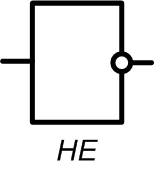
\includegraphics[width=.17\textwidth]{fig/not}
                }
            \end{array}
        \]
        <<$\textit{не}(x)$>> также обозначается: <<$\lnot x$>>, <<$\overline{x}$>>.
\end{enumerate}

Из $2^{2^2}=16$ функций двух аргументов далее рассматриваются лишь те, которые понадобятся в дальнейшем. 
\begin{itemize}
    \item $\textit{и}(x_1,x_2)$. Конъюнкция (\textit{И}, \textit{AND}). 
    \[
        \begin{array}{ccc}
            \begin{array}{cc|c}
                x_1&x_2&\textit{и}(x_1,x_2)\\
                \hline
                0&0&0\\
                0&1&0\\
                1&0&0\\
                1&1&1\\
                \hline
            \end{array}
            &&
            \raisebox{-.7\height}{
                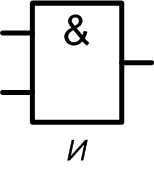
\includegraphics[width=.17\textwidth]{fig/and}
            }
        \end{array}
    \]
    
    Конъюнкция истинна только тогда, когда истинны оба аргумента. <<$\textit{и}(x,y)$>> также обозначается <<$x\land y$>>, <<$x \& y$>>, <<$x \cdot y$>> или <<$xy$>>.

    \item $\textit{или}(x_1,x_2)$. Дизъюнкция, \textit{ИЛИ}, \textit{OR}.
    \[
        \begin{array}{ccc}
            \begin{array}{cc|c}
                x_1&x_2&\textit{или}(x_1,x_2)\\
                \hline
                0&0&0\\
                0&1&1\\
                1&0&1\\
                1&1&1\\
                \hline
            \end{array}
            &&
            \raisebox{-.7\height}{
                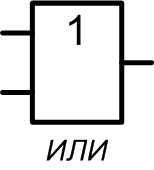
\includegraphics[width=.17\textwidth]{fig/or}
            }
        \end{array}
    \]
    
    Дизъюнкция ложна только тогда, когда ложны оба аргумента. <<$\textit{или}(x,y)$>> также обозначается <<$x \lor y$>>.

    \item $\textit{xor}(x_1,x_2)$. <<Исключающее или>>, <<сложение по модулю два>>, \textit{XOR} --- eXclusive OR.
    \[
        \begin{array}{ccc}
            \begin{array}{cc|c}
                x_1&x_2&\textit{xor}(x_1,x_2)\\
                \hline
                0&0&0\\
                0&1&1\\
                1&0&1\\
                1&1&0\\
                \hline
            \end{array}
            &&
            \raisebox{-.7\height}{
                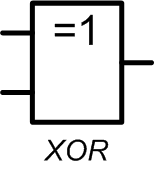
\includegraphics[width=.17\textwidth]{fig/xor}
            }
        \end{array}
    \]
    
    \emph{Исключающим или} функция названа потому, что $\textit{xor}(x_1,x_2)$ истинна, если истинно $x_1$ \emph{или} истинно $x_2$, \emph{но не} оба сразу. Проще запомнить эту функцию, как результат арифметического сложения двух бит с отброшенным переносом. <<$\textit{xor}(x,y)$>> также обозначается: <<$x \oplus y$>>.

    \item $\textit{если-то}(x_1,x_2)$. Импликация, \textit{ЕСЛИ-ТО}.
    \[
        \begin{array}{cc|c}
            x_1&x_2&\textit{если-то}(x_1,x_2)\\
            \hline
            0&0&1\\
            0&1&1\\
            1&0&0\\
            1&1&1\\
            \hline
        \end{array}
    \]
    
    Импликация является аналогом высказывания <<если $x_1$, то $x_2$>>. Оно ложно лишь тогда, когда посылка $x_1$ истинна, а следствие $x_2$ ложно. <<$\textit{если-то}(x,y)$>> также обозначается: <<$x \to y$>>.
    
    \item $\textit{и-не}(x_1,x_2)$. Штрих Шеффера, \textit{И-НЕ}.
    \[
        \begin{array}{ccc}
            \begin{array}{cc|c}
                x_1&x_2&\textit{и-не}(x_1,x_2)\\
                \hline
                0&0&1\\
                0&1&1\\
                1&0&1\\
                1&1&0\\
                \hline
            \end{array}
            &&
            \raisebox{-.7\height}{
                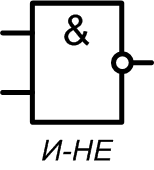
\includegraphics[width=.17\textwidth]{fig/notAnd}
            }
        \end{array}
    \]
    
    <<$\textit{и-не}(x,y)$>> также обозначается: <<$x\mid y$>>.

    \item $\textit{или-не}(x_1,x_2)$. Стрелка Пирса, \textit{ИЛИ-НЕ}.
    \[
        \begin{array}{ccc}
            \begin{array}{cc|c}
                x_1&x_2&\textit{или-не}(x_1,x_2)\\
                \hline
                0&0&1\\
                0&1&0\\
                1&0&0\\
                1&1&0\\
                \hline
            \end{array}
            &&
            \raisebox{-.7\height}{
                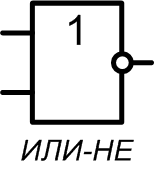
\includegraphics[width=.17\textwidth]{fig/notOr}
            }
        \end{array}
    \]
    
    <<$\textit{или-не}(x,y)$>> также обозначается: <<$x\uparrow y$>>.
\end{itemize}

В заключение упомянем такие достойные функции двух аргументов, как \emph{константы нуля} и \emph{единицы}, \emph{эквивалентность}, \emph{штрих Шеффера} и \emph{стрелку Пирса}. Их рассматривать не будем. 

Не имеет смысла рассматривать \emph{функции} трех и большего количества аргументов, в силу того, что их можно выразить \emph{формулой}, сконструированной из функций одного и/или двух аргументов.


\section{Формулы}

Формулой будем называть выражение 
\begin{equation}
    \label{eq:ch:alog:binform}
    f(t_1,\ldots,t_n),
\end{equation}
где аргумент $t_i$ --- подформула, т.е. либо аналогичного вида формула, либо переменная, принимающая одно из значений $0$, либо $1$.

Прежде чем найти значение формулы, нужно найти значения подформул, стоящих в аргументах.

\begin{exampl} Задача. Найти значение формулы 
\[
    \textit{или}(0,\textit{и}(\textit{не}(1), 1)).
\]
\end{exampl}
\begin{proof}[Решение] 
\(
    \textit{или}(0,\textit{и}(\textit{не}(1), 1))\Rightarrow
    \textit{или}(0,\textit{и}(0, 1))\Rightarrow
    \textit{или}(0,0)\Rightarrow 0
\)
\end{proof}

Функции произвольного количества аргументов можно конструировать на основе вышеназванных функций одного и двух аргументов. 
    \begin{exampl}\label{ex:ch:alog:f3arg} Функция трёх аргументов 
    \[
        g(x_1,x_2,x_3)=\textit{или}(x_1,\textit{и}(\textit{не}(x_2), x_3))
    \]
    задана формулой. Соответствующая формуле логическая схема приведена на рисунке \ref{fig::alog:formulae}.
\end{exampl}

\begin{figure}[!ht]
    \centering
    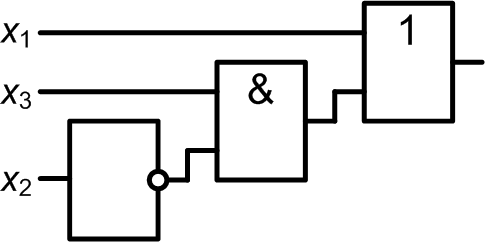
\includegraphics[width=.42\textwidth]{fig/formulae}
    \caption{Логическая схема $g(x_1,x_2,x_3)=\textit{или}(x_1,\textit{и}(\textit{не}(x_2), x_3))$}
    \label{fig::alog:formulae}
\end{figure} 

Кроме того, на практике всегда в формулах вместо обозначений функций используют символы \emph{операции}, например:
\begin{itemize}
    \item вместо <<$\textit{не}(x)$>> пишут <<$(\lnot x)$>> или <<$(\bar{x})$>>;
    \item вместо <<$\textit{и}(x,y)$>> пишут <<$(x \land y)$>>, <<$(x \& y)$>>,  <<$(x \cdot y)$>> или  <<$(xy)$>>;
    \item вместо <<$\textit{или}(x,y)$>> пишут <<$(x \lor y)$>>;
    \item вместо <<$\textit{xor}(x,y)$>> пишут <<$(x \oplus y)$>>;
    \item вместо <<$\textit{если-то}(x,y)$>> пишут <<$(x \to y)$>>.
\end{itemize}

Задавая приоритет операций (выше они перечислены в порядке убывания приоритета), лишние скобки опускают.
\begin{exampl} 
    <<$\lnot x\lor y\land z$>> то же самое, что <<$(\lnot x)\lor (y\land z)$>>.
\end{exampl}

\begin{exampl}
    Функция $g(x_1,x_2,x_3)$ из примера \ref{ex:ch:alog:f3arg}:
    \[
        g(x_1,x_2,x_3) = x_1 \lor \lnot x_2 \land x_3
    \]
\end{exampl}


\section{Основной логический базис}

Функции \emph{И}, \emph{ИЛИ}, \emph{НЕ} составляют \emph{основной логический базис}. Любую функцию можно выразить формулой на их основе. Эти логические связки часто используются в обыденной жизни.

Принцип конструирования любой функции в основном логическом базисе демонстрируется следующим примером.

\begin{exampl} Задача. Представить функцию $f(x_1,x_2,x_3)$ в основном логическом базисе.
    \[
        \begin{array}{ccc|c}
            x_1&x_2&x_3&f(x_1,x_2,x_3)\\
            \hline
            0&0&0&0\\
            0&0&1&0\\
            0&1&0&1\\
            0&1&1&0\\
            1&0&0&0\\
            1&0&1&0\\
            1&1&0&1\\
            1&1&1&0\\
            \hline
        \end{array}    
    \]
\end{exampl}
\begin{proof}[Решение]
    На наборе $x_1=0$, $x_2=1$, $x_3=0$ функция $f(x_1,x_2,x_3)$ должна равняться единице. При этом видно, что функция $f_2(x_1,x_2,x_3)=\overline{x_1}\land x_2 \land\overline{x_3}$ равняется единице только на этом наборе. $f(x_1,x_2,x_3)$ также должна равняться $1$ на наборе $x_1=1$, $x_2=1$, $x_3=0$. $f_6(x_1,x_2,x_3)=x_1\land x_2 \land\overline{x_3}$. Стало быть\footnote{Конечно, это решение можно оптимизировать. Вдумавшись, можно видеть, что от $x_1$ функция не зависит: $f(x_1,x_2,x_3)=x_2 \land\overline{x_3}$. Такое представление называется ДНФ --- дизъюнктивная нормальная форма. Оптимизация формул здесь не рассматривается} $f(x_1,x_2,x_3)=f_2(x_1,x_2,x_3)\lor f_6(x_1,x_2,x_3)=(\overline{x_1}\land x_2 \land\overline{x_3})\lor(x_1\land x_2 \land\overline{x_3})$.
\end{proof}

Оказывается, что основной логический базис избыточен. Например, функцию \emph{И} можно выразить через функции \emph{ИЛИ} и \emph{НЕ}. Действительно $x_1\land x_2 = \overline{\overline{x_1}\lor\overline{x_1}}$, в чём нетрудно убедиться непосредственной проверкой:
\[
    \begin{array}{c|cc|c}
        x_1\land x_2&x_1&x_2&\overline{\overline{x_1}\lor\overline{x_1}}\\
        \hline
        0&0&0&0\\
        0&0&1&0\\
        0&1&0&0\\
        1&1&1&1\\
        \hline
    \end{array}
\]

Впрочем, чтобы образовать базис, достаточно и одной функции. Например, функции \emph{стрелка Пирса} или \emph{штрих Шеффера} в одиночку образуют базис. И любую функцию можно выразить через одну из них. 

Для того, чтобы это доказать, достаточно выразить, например функции \textit{НЕ} и \textit{ИЛИ} через стрелку Пирса (см. схему на рисунке \ref{fig::alog:orByNotOr}):
\begin{itemize}
    \item \textit{НЕ}: $\lnot x=x\uparrow x$;
    \item \textit{ИЛИ}: $x\lor y=\lnot(x\uparrow y)=(x\uparrow y)\uparrow(x\uparrow y)$;
\end{itemize}

\begin{figure}[!ht]
    \centering
    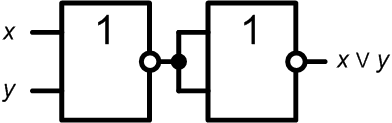
\includegraphics[width=.45\textwidth]{fig/orByNotOr}
    \caption{$x\lor y=\lnot(x\uparrow y)=(x\uparrow y)\uparrow(x\uparrow y)$}
    \label{fig::alog:orByNotOr}
\end{figure} 

Выбор базиса и эффективное упрощение формул в нём сильно влияют на стоимость создаваемых в итоге вычислительных устройств.


\section*{Задания}
\addcontentsline{toc}{section}{Задания}


\paragraph{Задания базового уровня}

\begin{enumerate}
    \item Доказать или опровергнуть утверждения:
    \begin{enumerate}
        \item $\overline{\overline{x}}=x$;
        \item $x\oplus 1=\overline{x}$;
        \item $x\oplus 0=x$;
        \item $x\oplus x=0$;
        \item $x\lor y = y\lor x$;
        \item $x\land y = y\land x$;
        \item $x\to y = \overline{x}\lor y$;
        \item $(x\lor y)\lor z = x\lor(y\lor z)$;
        \item $x\land (y\lor z) = (x\land y)\lor(x\land z)$;
        \item $x\lor (y\land z) = (x\lor y)\land(x\lor z)$;
        \item $\overline{x\lor y}=\overline{x}\land\overline{y}$;
    \end{enumerate}
    
    \item Сколько существует функций четырёх аргументов? Пяти?
    
    \item Выразить функцию \emph{ИЛИ} через функции \emph{И}, \emph{НЕ}.

    \item Выразить импликацию в основном логическом базисе.
    
    \item Построить таблицу истинности для функции:
    \begin{enumerate}
        \item $f(x)=x\to x$;
        \item $f(x,y)=\overline{\overline{x}\lor y}$;
        \item $f(x,y,z)=(\overline{x}\lor y)\land(\overline{y}\lor z)$.
    \end{enumerate}
    
    \item Записать формулу, используя знаки операций:
    \begin{enumerate}
        \item $\textit{или}(\textit{или}(a,b),\textit{и}(c,d))$;
        \item $\textit{не}(\textit{или}(a,\textit{или}(\textit{не}(b),c)))$;
        \item $\textit{xor}(\textit{не}(\textit{и}(c,\textit{если-то}(a,b))),d)$.
    \end{enumerate}
    
    Лишние скобки следует опустить.

    \item\label{en:ch:alog:logicVentils} На функциональных схемах логические элементы основного логического базиса изображаются так
    \begin{center}
        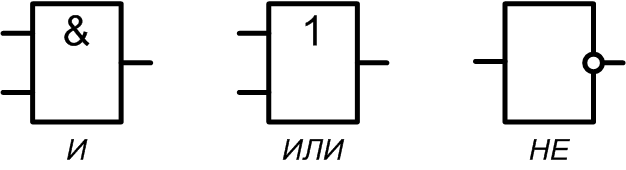
\includegraphics[width=.5\textwidth]{fig/logicVentils}
    \end{center}
    
    Нарисовать схему, соответствующую формуле:
    \begin{enumerate}
        \item $(x\lor y\lor z)\land\overline{x}$;
        \item $x\lor\overline{(y\land z)}$;
        \item $x\land\overline{\overline{y}\lor z}$;
        \item $\overline{x\land\overline{y\land\overline{z}}}$;
        \item $x\land y\land z\lor(\overline{x\land y})$;
        \item $x\oplus y$;
        \item $x\to (y\to z)$.
    \end{enumerate}
    
    Записать формулу, перейдя от знаков операций к обозначениям функций. Например, $x\land y$ соответствует $\textit{и}(x,y)$.
    
    \item\label{en:ch:alog:psum} Полусумматором называется логическая схема, принимающая на входе две двоичные цифры-слагаемые текущего разряда, а на выходе формирующая результат и перенос в следующий разряд. Задать формулы для результата и переноса в основном логическом базисе, и нарисовать схему из элементов, представленных в задании \ref{en:ch:alog:logicVentils} данного блока.
    
    \item Двоичным сумматором называется логическая схема, принимающая на входе две двоичные цифры-слагаемые текущего разряда и перенос из предыдущего разряда, а на выходе формирующая результат и перенос в следующий разряд. Сформировать сумматор на основе полусумматоров (см. задание \ref{en:ch:alog:psum} данного блока) и функций основного логического базиса. Сформировать из сумматоров схему, складывающую $4$-х разрядные числа.
    
\end{enumerate}


\paragraph{Программирование}
\begin{enumerate}
    \item Компьютерная память хранит двоичные данные блоками бит фиксированного размера --- \emph{байтами}. Будем считать, что байт --- это восемь бит. Процессоры также поддерживают логические операции, в которых в качестве оперендов выступают байты, при этом операции выполняются над битами соответствующих разрядов. Рассмотрим некоторые операторы языка C. 
    \begin{center}
        \begin{tabular}{c|l}
            \hline\hline
            Оператор C & Действие оператора\\
            \hline\hline
            \verb"x=y"  &Присвоить переменной \verb"x" значение \verb"y"\\
            \verb"x==y" &Сравнить значения переменных \verb"x" и \verb"y"\\
            \verb"~x"   &Битовое \emph{НЕ}\\
            \verb"x|y"  &Битовое \emph{ИЛИ}\\
            \verb"x&y"  &Битовое \emph{И}\\
            \verb"x^y"  &Битовое \emph{XOR}\\
            \verb"x<<n" &Сдвиг значения \verb"x" на \verb"n" бит влево\\
            \verb"x>>n" &Сдвиг значения \verb"x" на \verb"n" бит вправо\\
            \hline
        \end{tabular}
    \end{center}
    
    В качестве примера приведём фрагмент программы:
\begin{verbatim}    
    x  = 60; //00111100b
    y  = 90; //01011010b
    z1 = ~x;
    z2 = x|y;
    z3 = x&y;
    z4 = x^y;
    z5 = x<<1;
    z6 = x>>2;
\end{verbatim}

    И результаты его выполнения:
    \begin{center}
        \begin{tabular}{lcccccccccc}
                     &&\small{7}&\small{6}&\small{5}&\small{4}&\small{3}&\small{2}&\small{1}&\small{0}& \\ \cline{3-10}
            \verb"x"    &\multicolumn{1}{c|}{}  &0&0&1&1&1&1&0&0&\multicolumn{1}{|c}{}\\ \cline{3-10}
            \verb"y"    &\multicolumn{1}{c|}{}  &0&1&0&1&1&0&1&0&\multicolumn{1}{|c}{}\\ \cline{3-10}
            \\ \cline{3-10}
            \verb"z1 = ~x"   &\multicolumn{1}{c|}{}  &1&1&0&0&0&0&1&1&\multicolumn{1}{|c}{}\\ \cline{3-10}
            \verb"z2 = x|y"  &\multicolumn{1}{c|}{}  &0&1&1&1&1&1&1&0&\multicolumn{1}{|c}{}\\ \cline{3-10}
            \verb"z3 = x&y"  &\multicolumn{1}{c|}{}  &0&0&0&1&1&0&0&0&\multicolumn{1}{|c}{}\\ \cline{3-10}
            \verb"z4 = x^y"  &\multicolumn{1}{c|}{}  &0&1&1&0&0&1&1&0&\multicolumn{1}{|c}{}\\ \cline{3-10}
            \verb"z5 = x<<1" &\multicolumn{1}{c|}{}  &0&1&1&1&1&0&0&0&\multicolumn{1}{|c}{}\\ \cline{3-10}
            \verb"z6 = x>>2" &\multicolumn{1}{c|}{}  &0&0&0&0&1&1&1&1&\multicolumn{1}{|c}{}\\ \cline{3-10}
        \end{tabular}
    \end{center}
    
    Задания.
    \begin{enumerate}
        \item Чему равно \verb"(7&3)|12"?
        \item Чему равно \verb"(90&0xF)<<(~0xFC)"?
        \item Напишите программу, записывающую значение $(1010)_2$ в старшие $4$ бита байта \verb"x".
        \item Напишите программу, проверяющую установлен ли \verb"n"-й бит в байте \verb"x"?
        \item Напишите программу, устанавливающую \verb"n"-й бит в байте \verb"x" в $1$.
        \item Напишите программу, сбрасывающую \verb"n"-й бит в байте \verb"x" в $0$.
        \item Напишите программу, меняющую местами старшую и младшую тетрады\footnote{Тетрада --- четыре бита} байта.
        \item Напишите программу, выполняющую циклический сдвиг байта \verb"x" на \verb"n" бит вправо.
        \item Напишите программу, инвертирующую младшую тетраду байта \verb"x".
    \end{enumerate}
\end{enumerate}


\paragraph{Философия}
\begin{enumerate}
    \item Функция \emph{штрих Шеффера}, называемая также \emph{И-НЕ}, образует базис. Обозначается она символом операции $x\mid y$:
    \[
        \begin{array}{cc|c}
            x_1&x_2&x_1\mid x_2\\
            \hline
            0&0&1\\
            0&1&1\\
            1&0&1\\
            1&1&0\\
            \hline
        \end{array}
    \]
    выразить через неё функции основного логического базиса.

    \item Функция \emph{стрелка Пирса}, называемая также \emph{ИЛИ-НЕ}, образует базис. Обозначается она символом операции $x\uparrow y$:
    \[
        \begin{array}{cc|c}
            x_1&x_2&x_1\uparrow x_2\\
            \hline
            0&0&1\\
            0&1&0\\
            1&0&0\\
            1&1&0\\
            \hline
        \end{array}
    \]
    выразить через неё функции основного логического базиса.
    
\end{enumerate}

 %Алгебра логики
    \chapter{Множества} 

%sets: prefix
Множество --- фундаментальное понятие всей дискретной математики. Для углубленного изучения рекомендуются \cite{bib:sudoplatov:discrmath, bib:haggard:discrmathprogrammer, bib:novic:discrmathprogrammer}.


\section{Базовые понятия теории множеств}

Множество --- фундаментальное понятие. Оно не определимо явно. Под множеством $M$ подразумевается совокупность некоторых объектов, которые будут называться \emph{элементами} множества $M$. Принадлежность элемента $x$ множеству $M$ обозначается символом $\in$. Пишут $x\in M$, если $x$ является элементом множества $M$, и $x\not\in M$, если $x$ не является элементом $M$. 

Чтобы задать множество, нужно указать какие элементы ему принадлежат. Для этого существует несколько способов.
\begin{itemize}
    \item Явным перечислением элементов:\[\{a_1,a_2,\ldots,a_n\}.\]
    \item Характеристическим предикатом:\[\{x|P(x)\}.\]
    \item Порождающей процедурой:\[\{x|x=f\}.\]
\end{itemize}

\begin{exampl} Способы задания множеств

    \begin{itemize}
        \item Явное перечисление:$M=\{a,b,c,d\}$. Элементами множества могут быть другие множества $M=\{1,\{2,3\},\{4,5\}\}$.
        \item Характеристический предикат, задающий множество четных чисел:$M=\{x|x\text{---четное}\}$.
        \item Порождающая процедура:$M=\{n|for\ n=1\ to\ 4\ do\ yeld\ n;\}$. Генерируется множество $M=\{1,2,3,4\}$.
    \end{itemize}
\end{exampl}

%Характеристический предикат является хорошим способом задать множество, но с его формулировкой нужно быть очень осторожным. Рассмотрим, например, парадокс Рассела. Рассмотрим множество всех множеств, не содержащих себя в качестве элемента.
%\[Y=\{X|X\not\in X\}\]
%Зададимся вопросом является ли $Y$ элементом самого себя? Если $Y$ не содержит себя в качестве элемента, то оно по определению должно являться элементом самого себя. Если $Y$ является элементом самого себя, то в этом случае по условию оно само себя в качестве элемента содержать не может.

Существуют некоторые множества, для которых приняты стандартные обозначения:
\begin{itemize}
    \item $\emptyset=\{\}$ --- пустое множество;
    \item $\mathbb{N}=\{0,1,2,\ldots\}$ --- множество натуральных чисел;
    \item $\mathbb{Z}=\{0,\pm 1,\pm 2,\ldots\}$ --- множество целых чисел;
    \item $\mathbb{Q}$ --- множество всех рациональных дробей;
    \item $\mathbb{P}$ --- множество простых чисел;
    \item $\mathbb{R}$ --- множество вещественных (действительных) чисел;
    \item $\mathbb{C}$ --- множество комплексных чисел.
\end{itemize}

Множество $A$ \emph{содержится} в множестве $B$ (множество $B$ \emph{включает} множество $A$), если каждый элемент $A$ есть элемент $B$. Такое отношение между множествами $A$ и $B$ называется \emph{отношением нестрогого включения} и обозначается символом $\subseteq$:
\[A\subseteq B, \text{если\ } (x\in A)\Rightarrow (x\in B).\]
В этом случае $A$ --- \emph{подмножество}, а $B$ --- \emph{надмножество}. Запись $B\supseteq A$ обозначает то же, что и запись $A\subseteq B$.

Множество $A$ называется \emph{собственным} подмножеством множества $B$, если $A$ является подмножеством множества $B$, и если $B$ не является подмножеством $A$. Такое отношение между множествами $A$ и $B$ обозначается символом \emph{отношения строгого включения} $\subset$:
\[A\subset B,\text{если $(A\subseteq B)\land(B\not\subseteq A)$},\]
где $\land$ --- обозначение
\footnote{
    В различных литературных источниках основные логические связки обозначаются по разному. Например.
    \begin{itemize}
        \item Объединение условий по <<И>>: <<$\&$>>, <<$\land$>>. Перечисление условий через запятую также считается объединением по <<И>>:$A,B,C$, например, соответствует $A\land B\land C$.
        \item Объединение условий по <<ИЛИ>>: <<$\lor$>>, <<$|$>>, <<$||$>>.
        \item Логическое отрицание условия $A$: $\lnot A$, $\bar{A}$.
    \end{itemize}
} объединения логических условий по <<И>>. Запись $B\supset A$ означает то же, что и запись $A\subset B$.
  
Для любого множества $M$ справедливо:
\begin{itemize}
    \item $M\subseteq M$;
    \item $\emptyset\subseteq M$.
\end{itemize}

Множества $A$ и $B$ равны (обозначается $A=B$), если $A$ подмножество $B$ и $B$ подмножество $A$:

\begin{equation}
    \label{eq:ABSetEquality}
    (A=B)\Leftrightarrow(A\subseteq B\land B\subseteq A).
\end{equation}

Множества $A$ и $B$ находятся в \emph{общем положении} (обозначается $\text{ОП}(A,B)$), если одновременно выполняются три условия (см. рис.\ref{fig:commonABset}):
\begin{enumerate}
    \item $\exists x (x\in A \land  x\not\in B)$,
    \item $\exists y (y\in B \land  y\not\in A)$,
    \item $\exists z (z\in A \land  z\in B)$.
\end{enumerate}

\begin{figure}
    \centering
    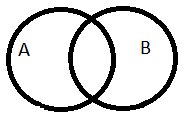
\includegraphics{fig/commonABset}
    \caption{Общее положение множеств $A$ и $B$}
    \label{fig:commonABset}
\end{figure} 

Два множества $A$ и $B$ могут находится лишь в одном из следующих отношений:
\begin{enumerate}
    \item $A=B$;
    \item $A\subset B$;
    \item $A\supset B$;
    \item $A\cup B = \emptyset$, т.е. $A$ и $B$ не имеют общих элементов;
    \item $\text{ОП}(A,B)$, т.е. $A$ и $B$ находятся в общем положении. 
\end{enumerate}

Количество элементов в \emph{конечном} множестве $A$ называют \emph{мощьностью конечного множества} и обозначают $|A|$.

Множество всех подмножеств множества $M$ называется \emph{булеаном} и обозначается $2^M$:
\[2^M=\{A|A\subseteq M\}.\]
Для конечного множества $M$ справедливо $\left|2^M\right|=2^{\left|M\right|}$.

В алгебре множеств вводятся следующие \emph{основные} операции над множествами (см. рис. \ref{fig:mainSetOperations}):
\begin{enumerate}
    \item объединение:\[A\cup B=\{x|x\in A \lor x\in B\};\]
    
    \item пересечение:\[A\cap B=\{x|x\in A \land x\in B\};\]
    
    \item дополнение:\[\overline{A}=\{x|x\not\in A\}.\]
\end{enumerate}

\begin{figure}
    \centering
    \begin{tabular}{||c||c||c||}
        \hline\hline
        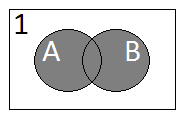
\includegraphics[width=.2\textwidth]{fig/ABsetOr}
            & 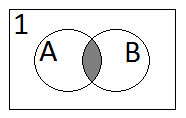
\includegraphics[width=.2\textwidth]{fig/ABsetAnd}
                & 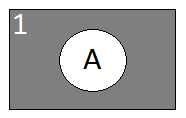
\includegraphics[width=.2\textwidth]{fig/AsetNot}\\
        $A\cup B$ 
            & $A\cap B$
                & $\overline{A}$\\
        \hline\hline
    \end{tabular}
    \caption{\emph{Основные} операции над множествами на диаграммах Венна}
    \label{fig:mainSetOperations}
\end{figure}

Кроме того, при выполнении преобразований над множествами удобно ввести следующие \emph{дополнительные} операции (см. рис. \ref{fig:slaveSetOperations}):
\begin{enumerate}
    \item разность:\[A\backslash B=A\cap\overline{B}=\{x|x\in A \land x\not\in B\};\]
    
    \item симметрическая разность:
    \[
    \begin{split}
        A\Delta B=(A\backslash B)\cup(B\backslash A)=(A\cup B)\backslash(A\cap B)=\\
        =\{x|(x\in A \land x\not\in B)\lor(x\not\in A\land x\in B)\}.
    \end{split}
    \]
\end{enumerate}

\begin{figure}
    \centering
    \begin{tabular}{||c||c||}
        \hline\hline
        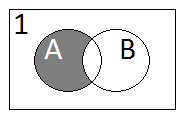
\includegraphics[width=.2\textwidth]{fig/ABsetSub}
            & 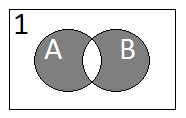
\includegraphics[width=.2\textwidth]{fig/ABsetSymSub}\\
        $A\backslash B$ 
            & $A\Delta B$\\
        \hline\hline
    \end{tabular}
    \caption{\emph{Дополнительные} операции над множествами на диаграммах Венна}
    \label{fig:slaveSetOperations}
\end{figure}

Операции над множествами обладают следующими свойствами:
\begin{enumerate}
    \item идемпотентность:
    \[A\cup A=A,A\cap A=A;\]
    
    \item коммутативность:
    \[A\cup B=B\cup A,A\cap B=B\cap A;\]
    
    \item ассоциативность:
    \[(A\cup B)\cup C=A\cup(B\cup C),(A\cap B)\cap C=A\cap(B\cap C);\]
    
    \item дистрибутивность:
    \[A\cup(B\cap C)=(A\cup B)\cap(A\cup C),A\cap(B\cup C)=(A\cap B)\cup(A\cap C);\]
    
    \item законы де Моргана:
    \[
        \overline{A\cap B}=\overline{A}\cup\overline{B},
        \overline{A\cup B}=\overline{A}\cap\overline{B};
    \]
    
    \item поглощение:
    \[(A\cup B)\cap A=A,(A\cap B)\cup A=A;\]
    
    \item свойства нуля (пустого множества $\emptyset$):
    \[(A\cup \emptyset)=A,(A\cap \emptyset)=\emptyset;\]
    
    \item свойства единицы (универсального множества $1$):
    \[(A\cup 1)=1,(A\cap 1)=A;\]
    
    \item инволютивность:
    \[\overline{\overline{A}}=A;\]
        
    \item свойства дополнения:
    \[
        \overline{A}\cup A=1,
        \overline{A}\cap A=\emptyset;
    \]
    
    \item выражение разности:
    \[
        A\backslash B=A\cap\overline{B}.
    \]
\end{enumerate}

Докажем некоторые утверждения
\begin{exampl} 
    Докажем закон инволютивности: $\overline{\overline{A}}=A$. 
\end{exampl}
\begin{proof}
    Исходя из определения равенства (формулы \eqref{eq:ABSetEquality}), докажем, что $\overline{\overline{A}}\subseteq A$ и $A\subseteq\overline{\overline{A}}$.
    \begin{enumerate}
        \item $\overline{\overline{A}}\subseteq A$. Допустим, $x\in\overline{\overline{A}}$, тогда $x\not\in\overline{A}$. Это значит, что $x\in A$.
        \item $A\subseteq\overline{\overline{A}}$. Допустим, $x\in A$, тогда $x\not\in\overline{A}$. Стало быть $x\in\overline{(\overline{A})}$.
    \end{enumerate}
\end{proof}

\begin{exampl} 
    Докажем (по формуле \eqref{eq:ABSetEquality}) закон де Моргана для случая $\overline{A\cup B}=\overline{A}\cap\overline{B}$. 
\end{exampl}
\begin{proof}
    Докажем, что $\overline{A\cup B}\subseteq\overline{A}\cap\overline{B}$ и $\overline{A}\cap\overline{B}\subseteq\overline{A\cup B}$.
    \begin{enumerate}
        \item $\overline{A\cup B}\subseteq\overline{A}\cap\overline{B}$. Возьмем элемент $x\in \overline{A\cup B}$. Делаем вывод, что $x\not\in A\cup B$. Поскольку элемент $x$ не входит в объединение множеств, то он не может входить ни в одно из этих множеств. Поэтому справедливо $x\not\in A$ и $x\not\in B$. То есть $x\in\overline{A}$ и $x\in\overline{B}$, по определению $x\in\overline{A}\cap\overline{B}$.
        \item $\overline{A}\cap\overline{B}\subseteq\overline{A\cup B}$. Возьмем элемент $x\in\overline{A}\cap\overline{B}$. Тогда $x\in\overline{A}$, а значит $x\not\in A$. Аналогично делаем вывод, что $x\not\in B$. Стало быть $x\not\in(A\cup B)$, а значит $x\in\overline{A\cup B}$.
    \end{enumerate}
\end{proof}

\begin{exampl}
    Докажем (по формуле \eqref{eq:ABSetEquality}), что операция разности множеств выражается через основные операции алгебры множеств так: $A\backslash B=A\cap\overline{B}$.
\end{exampl}
\begin{proof}
    Докажем, что $A\backslash B\subseteq A\cap\overline{B}$ и $A\cap\overline{B}\subseteq A\backslash B$.
    \begin{enumerate}
        \item $A\backslash B\subseteq A\cap\overline{B}$. Возьмем $x\in A\backslash B$, тогда по определению справедливо $x\in A$ и $x\not\in B$. То есть $x\in A$ и $x\in\overline{B}$. По определению $x\in A\cap\overline{B}$.
        \item $A\cap\overline{B}\subseteq A\backslash B$. Возьмем элемент $x\in A\cap\overline{B}$. Тогда справедливо $x\in A$ и $x\in\overline{B}$. То есть справедливо $x\in A$ и $x\not\in B$. По определению $x\in A\backslash B$.
    \end{enumerate}
\end{proof}

Следует отметить, что набор \emph{основных} операций алгебры множеств избыточен. Необходимым и достаточным минимумом операций являются, например, операции отрицания $\bar{~}$ и пересечения $\cap$. При этом операция объединения выражается через них: $A\cup B=\overline{\overline{A}\cap\overline{B}}$. Любую операцию алгебры множеств можно свести к указанным двум.

Впрочем, оказывается, что любую операцию алгебры множеств можно выразить лишь одной \emph{дополнительной} операцией вычитания:
\begin{itemize}
    \item $\overline{A}=1\backslash A$;
    \item $A\cap B=A\backslash (1\backslash B)$;
    \item $A\cup B=1\backslash((1\backslash A)\backslash B)$.    
\end{itemize}

Покажем, как на основе свойств операций над множествами можно проводить аналитические преобразования.
\begin{exampl}[Аналитические преобразования множеств]
\[
\begin{split}
A\backslash ((A\cup B)\backslash B) = A\cap\overline{((A\cup B)\cap\overline{B})}=\\
=A\cap(\overline{(A\cup B)}\cup\overline{\overline{B}})=A\cap((\overline{A}\cap\overline{B})\cup B)=\\
=A\cap((\overline{A}\cup B)\cap\underbrace{(\overline{B}\cup B)}_1)=A\cap (\overline{A}\cup B) = \underbrace{(A\cap\overline{A})}_\emptyset\cup(A\cap B)=\\
=A\cap B
\end{split}
\]
\qed
\end{exampl}

В завершение дадим несколько определений.

$\mathcal{E}=\{E_i|i\in\mathbb{N}\land E_i\subset M\}$ называется \emph{семейством} подмножеств множества $M$. Cемейство $\mathcal{E}$ называют \emph{покрытием} множества $M$, если каждый элемент $M$ содержится хотя бы в одном $E_i$:
\[
M\subseteq\bigcup_{i\in\mathbb{N}}E_i
\Leftrightarrow
\forall x\in M~\exists i\in\mathbb{N}~x\in E_i
\]

Семейство $\mathcal{R}$ называют \emph{дизъюнктивным} (или \emph{разбиением}), если множества $E_i$ попарно не пересекаются:
\[
\forall i,j\in\mathbb{N}~i\neq j\Rightarrow E_i\cap E_j=\emptyset
\]

Упорядоченную последовательность из $n$ элементов $(x_1,x_2,\ldots,x_n)$ будем называть \emph{кортежем} длины $n$. Элемент $x_i$ называется $i$-й \emph{координатой} кортежа. Два кортежа длины $n$: $(x_1,x_2,\ldots,x_n)$ и $(y_1,y_2,\ldots,y_n)$ равны тогда и только тогда, когда $x_1=y_1$,$x_2=y_2$,\ldots,$x_n=y_n$.

\emph{Декартовым} (прямым) произведенем множеств $A_1,A_2,\ldots,A_n$ называется множество 
\[\{(x_1,x_2,\ldots,x_n)|x_1\in A_1,x_2\in A_2,\ldots,x_n\in A_n\},\]
обозначаемое через 
\[A_1\times A_2\times\cdots\times A_n \text{~или~} \prod_{i=1}^{n}A_i.\]

Необходимо отметить, что $A\times B\neq B\times A$. 

Если $A_1=A_2=\ldots=A_n=A$, то множество $A_1\times A_2\times\cdots\times A_n$ называется $n$-й степенью множества $A$  и обозначается как $A^n$. По определению положим $A^0=\{\emptyset\}$.

\begin{exampl}
    Для множеств $A=\{a,b\}$ и $B=\{1,2\}$ имеем:
    \begin{itemize}
        \item $A\times B=\{(a,1),(b,1),(a,2),(b,2)\}$;
        \item $B\times A=\{(1,a),(1,b),(2,a),(2,b)\}$;
        \item $A\times A=A^2=\{(a,a),(a,b),(b,a),(b,b)\}$.
    \end{itemize}
    \qed
\end{exampl}

\begin{exampl}Щахматная доска.
    Пусть 
    \[
        A=\{a,b,c,d,e,f,g,h\},
        B=\{1,2,3,4,5,6,7,8\},
    \]
            тогда множество пар $(x,y)\in A\times B$ --- множество клеток шахматной доски.
    \qed
\end{exampl}

%TODO представление множеств в компьютере
%Множество из n>8 элементов. Представляется массивом байт. Написать алгоритм проверки наличия m-го элемента множества.
%Массив из скольки байт потребуется для представления $n$-элементного множества. Следует использовать операцию целочисленного деления 


\section*{Задания}
\addcontentsline{toc}{section}{Задания}

\begin{enumerate}
    \item Перечислить элементы указанных множеств. Определить мощность каждого множества.
    \begin{enumerate}
        \item $\emptyset$
        
        \item $\{\emptyset\}$
        
        \item $\{a,\{b,c\},d\}$
        
        \item $\{p|p\in \mathbb{P} \land 7\leq p\leq 30\}$
        
        \item $2^{\emptyset}$
        
        \item $2^{\{1,\{2,3\},\{4,5\}\}}$
        
        \item Числа Фибоначчи определяются рекурсивно так: 
        \[f(k)=
            \begin{cases}
            f(0)=1,\\
            f(1)=1,\\
            f(k)=f(k-1)+f(k-2),\text{при $k\in\mathbb{N}\land k>1$}.
            \end{cases}
        \]
        Определить $\{n|n=f(k),k\in\mathbb{N},4\leq n\leq 40\}$        
    \end{enumerate}
    
    \item Привести три возможных описания элементов множества $\{2,5,8,11,14\}$
    
    \item Задать множество точек, лежащих на сторонах треугольника с вершинами $A(0,0),B(0,3),C(4,0)$.
    
    \item Перечислить элементы следующих множеств.
    \begin{enumerate}
        \item $\{x|x\in\mathbb{Z}\land 6x^2+x-1=0\}$
        \item $\{x|x\in\mathbb{R}\land 6x^2+x-1=0\}$
        \item $\{x|x\in\mathbb{C}\land x^2+2x+2=0\}$
    \end{enumerate}
    
    \item Указать в каких отношениях находятся множества
    \begin{enumerate}
        \item $\{0,1\}$ и $\{2,3\}$
        \item $\{0,1\}$ и $\{0,1,2,3\}$
        \item $\{0,1,1\}$ и $\{1,0\}$
        \item $\{-1,0,1\}$ и $\mathbb{N}$
        \item $\mathbb{Z}$ и $\mathbb{R}$
        \item $\mathbb{C}$ и $\mathbb{R}$
        \item $\mathbb{Z}\backslash\{n|n=-k\land k\in\mathbb{N}\}$ и $\mathbb{N}$
    \end{enumerate}
    
    \item Даны множества $A=\{2,5,6,7\}$, $B=\{1,4,6,7\}$, $C=\{3,4,5,7\}$. Найти
    \begin{enumerate}
        \item $A\cap B$
        \item $A\cup B$
        \item $A\cap \overline{C}$
        \item $(A\cup B)\cap C$
        \item $A\backslash B$
        \item $A\Delta B = (A\cap \overline{B})\cup(B\cap\overline{A})$
    \end{enumerate}
    
    \item Рассмотрим три подмножества слов из словаря русского языка:
    \[A=\{x|x\text{---слово, стоящее перед словом <<собака>>}\}\]
    \[B=\{x|x\text{---слово, стоящее после слова  <<кошка>>}\}\]
    \[C=\{x|x\text{---слово, содержащее удвоенную букву}\}\]
    Какие из следующих выражений истинны?
    \begin{enumerate}
        \item $C\subset(A\cup B)$
        \item $\text{<<бассейн>>}\in (\overline{B}\cap C)$
        \item $\text{<<лассо>>}\in (B\Delta C)$
        \item $A\cap B=\emptyset$
    \end{enumerate}
    Опишите словесно свойства элементов следующих множеств:
    \begin{enumerate}
        \item $A\cap B \cap C$
        \item $(A\cup B)\cap \overline{C}$
    \end{enumerate}
    
    \item Пусть $A=\{n|n\in \mathbb{N} \land n=2k+1 \land k\in \mathbb{N}\}$,$B=\{n|n\in \mathbb{N} \land n=4k+1 \land k\in \mathbb{N}\}$. Доказать: 
    \begin{enumerate}
        \item $35\in A$
        \item $35\not\in B$
        \item $B\subseteq A$
        \item $B\subset A$
    \end{enumerate}
    
    \item Для множества $\{1,2,3,4\}$ постройте упорядоченный набор подмножеств, каждое последующее из которых отличается в одном элементе от предыдущего.
    
    \item Проиллюстрируйте диаграммами Венна для множеств $A,B,C$, находящихся в общем положении (см. рис. \ref{fig:commonABCset}).
    \begin{enumerate}
        \item $(A\backslash B)\cap C$
        \item $(A\backslash B)\cup C$
        \item $(A\backslash B)\cup (A\cap B)$
        \item $(A\cup B \cup C)\backslash(A\cap B\cap C)$
        \item $((A\cap B)\cup(A\cap C)\cup(B\cap C))\backslash(A\cap B\cap C)$
        \item $A\cap(\overline{B\cup C})$
    \end{enumerate}
    
    \item Записать эквивалентное выражение для выражения.
    \begin{enumerate}
        \item $A\cup B$, используя только операции $\cap,\bar{~}$.
        \item $A\backslash(B\cup C)$, используя только операции $\cap,\bar{~}$.
        \item $A\Delta B$, используя только операции $\cup,\bar{~}$.
        \item $\overline{A}$, используя только операцию $\backslash$.
        \item $A\cup B$, используя только операцию $\backslash$.
    \end{enumerate}
    
    \item Общее положение множеств $A,B,C$ изображено на диаграмме Венна (рис. \ref{fig:commonABCset}). Выразить формулами подмножества, изображенные на рис. \ref{fig:sets:ABCsubsets}
    
    \begin{figure}[h]
        \centering
        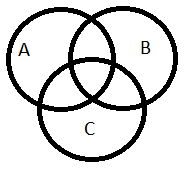
\includegraphics{fig/commonABCset}
        \caption{Общее положение множеств $A,B,C$}\label{fig:commonABCset}
    \end{figure} 
    
    \begin{figure}[!ht]
        \centering
        \begin{tabular}{||c||c||c||c||}
        \hline\hline
        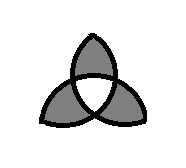
\includegraphics[width=.2\textwidth]{fig/ABCsubset1}
            & 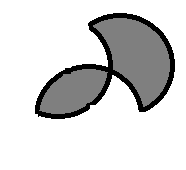
\includegraphics[width=.2\textwidth]{fig/ABCsubset2}
                & 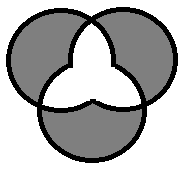
\includegraphics[width=.2\textwidth]{fig/ABCsubset3}
                    & 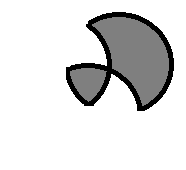
\includegraphics[width=.2\textwidth]{fig/ABCsubset4}
                        \\
        а)  &б) &в) &г) \\ 
        \hline\hline
        \end{tabular}
        \caption{Подмножества общего положения $A,B,C$ на рис. \ref{fig:commonABCset}}
        \label{fig:sets:ABCsubsets}
    \end{figure} 
    
    \item Доказать, что на рисунке \ref{fig:sets:commonABCDset} изображено общее положение четырёх множеств. Обосновать, почему четырьмя кругами такое общее положение изобразить не получится?
    \begin{figure}[!ht]
        \centering
        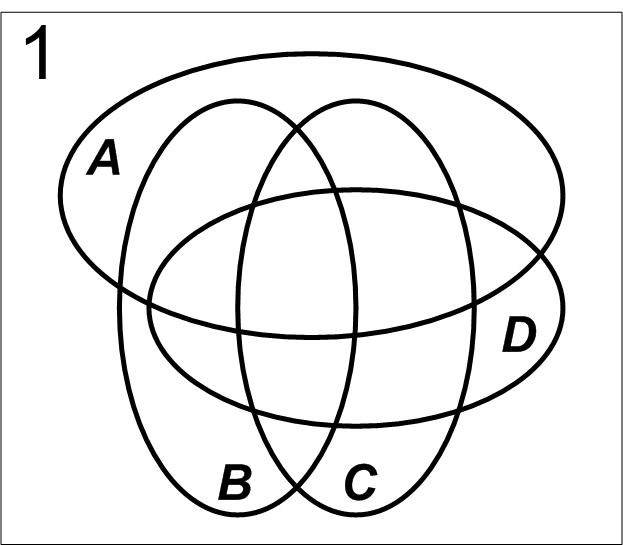
\includegraphics[width=.3\textwidth]{fig/commonABCDset}
        \caption{Общее положение четырёх множеств}
        \label{fig:sets:commonABCDset}
    \end{figure} 
    
    \item Доказать, что 
    \begin{enumerate}
        \item $(A\cap B)\cup A=A$
        \item Если $A\subseteq B$ или $A\subseteq C$, то $A\subseteq B\cup C$
        \item $(A\subseteq B)\Leftrightarrow (A\cap B=A)$
        \item $(A\subseteq B)\Leftrightarrow (\overline{B}\subseteq\overline{A})$
        \item $(A=B)\Leftrightarrow (\overline{A}=\overline{B})$
    \end{enumerate}
    
    \item Для $n$-элементного множества $A=\{a_1,\ldots,a_n\}$ оценить количество.
    \begin{enumerate}
        \item $n$-элементных кортежей, координаты которых принимают значения элементов $A$. Элементов множества $\{(x_1,\ldots,x_n)|x_1\in A,\ldots,x_n\in A\}$.
        
        \item $n$-элементных кортежей, координаты которых принимают значения элементов $A$, и при этом попарно различны. Элементов множества $\{(x_1,\ldots,x_n)|x_1\in A,\ldots,x_n\in A,\forall i,j i\neq j x_i\neq x_j, 1\leq i,j\leq n\}$.
        
        \item $m$-элементных кортежей ($m\leq n$), координаты которых принимают значения элементов $A$, и при этом попарно различны. Элементов множества $\{(x_1,\ldots,x_n)|x_1\in A,\ldots,x_n\in A,\forall i,j i\neq j x_i\neq x_j, 1\leq i,j\leq m\}$.
        
        \item $m$-элементных подмножеств множества $A$.
    \end{enumerate}
    
    \item Найти:
    \begin{enumerate}
        \item для множества $\{1,2,3,4\}$ все возможные двухэлементные подмножества;
        \item для множества $\{1,2,3,4\}$ все возможные трехэлементные подмножества;
        \item для множества $\{1,2,3\}$ все возможные трехэлементные кортежи, содержащие взаимно различные элементы $M$;
        \item для множества $\{1,2,3,4\}$ все возможные двухэлементные кортежи, содержащие взаимно различные элементы $M$;
    \end{enumerate}
    
    \item Определить количество $m$-элементных подмножеств $n$-элементного множества $\binom{m}{n}$. Сколько двухэлементных подмножеств 10 элементного множества? Чему равняется сумма $\sum_{i=0}^n \binom{i}{n}$?
    
    \item Является ли семейство $\mathcal{E}$ покрытием множества $M$? Дизьюнктивным покрытием (разбиением)?
    \begin{enumerate}
        \item $\mathcal{E}=\{\{a\},\{b,c\},\{c,d\}\}$, $M=\{a,b,c\}$.
        \item $\mathcal{E}=\{\{a\},\{b,c\},\{a,c\}\}$, $M=\{a,b,c\}$.
        \item $\mathcal{E}=\{\{a,b\},\{c\}\}$, $M=\{a,b,c\}$.
        \item $M=\mathbb{C}$,
        \[
        \begin{split}
            \mathcal{E}=\{
                \{a+b\cdot i|a,b\in\mathbb{R}\land b>0\land i=\sqrt{-1}\},\\
                \{a+b\cdot i|a,b\in\mathbb{R}\land b<0\land i=\sqrt{-1}\}
            \}.
        \end{split}
        \]
    \end{enumerate}
    
    \item Выполнить аналитические преобразования, применяя законы алгебры множеств.
    \begin{enumerate}
        \item $A\backslash((A\cup B)\backslash B)$
        \item $(A\backslash B)\cup(A\cap B)$
        \item $(A\cup B)\cap(A\cup\overline{B})\cap(\overline{A}\cup B)$
        \item $(A\cup (A\cap B))\cup(B\cap C)\cup(\overline{A}\cup C)$
        \item $A\cup\overline{(B\backslash\overline{A})}$
        \item $(A\cap B\cap C)\cup(\overline{A}\cap B\cap C)\cup\overline{B}\cup\overline{C}$
        \item $((A\cup B)\cap C)\cup(\overline{A}\cap C)\cup\overline{(\overline{B}\cup C)}$
        \item $(C\backslash(B\cap C))\cup((B\cap C)\cap(\overline{B}\cup\overline{C}))$
        \item $(\overline{A}\cup(A\cap B))\cup(\overline{B}\cup(A\cap B))$
        \item $A\cap\overline{((A\cup B)\cap\overline{B})}$
        \item $((A\cap B)\cup(A\cap\overline{C}))\cup((B\cup\overline{C})\cap\overline{A})$
    \end{enumerate}
\end{enumerate}
 %Множества
    \chapter{Регулярные множества и выражения}

В своё время регулярные выражения были прорывом в технике обработки текстов. И они не теряют своих позиций со временем. Регулярные выражения являются частью синтаксиса многих языков программирования\footnote{Например, perl}, в остальных же языках регулярные выражения доступны через функции стандартных библиотек. Более того, так как основным инструментом программиста является текстовый редактор, то практически все достойные внимания среды разработки поддерживают поиск и замену на основе регулярных выражений. Начнем с небольшого теоретического введения. Почерпнуть информацию о регулярных множествах и выражениях можно из \cite{bib:serebryakov:programminglang}.


\section{Формальное определение регулярных множеств и выражений}
Множество --- это фундаментальное, неопределяемое понятие математики. Можно сказать, что множество --- это любая определенная совокупность объектов. Объекты, из которых составлено множество, называются его элементами. Элементы множества различны и отличимы друг от друга. Если $x$ является элементом множества $M$, то говорят что $x$ принадлежит множеству $M$ и сей факт обозначается $x\in M$. В противном случае говорят, что $x$ не принадлежит множеству $M$ и обозначается $x\not\in M$. Если множество небольшое, то его можно задать простым перечислением элементов. Обычно элементы заключают в фигурные скобки и разделяют запятыми. Например, $1\in\{0,1,2\}$, а $3\not\in\{0,1,2\}$. 

Когда множество достаточно велико, то его задают с помощью условия, определяющего принадлежность элемента множеству или задают алгоритм, порождающий элементы множества. Например, множество целых чисел от одного до тысячи можно задать так $\{n|n\text{целое и\ } 1\leq n\leq 1000\}$. Множество не содержащее ни одного элемента, называется пустым и обозначается $\emptyset$. Объединением двух множеств $A$ и $B$ (обозначается $A\cup B$) называется множество, содержащее элементы обоих множеств: $A\cup B=\{x|x\in A\lor x\in B\}$, где $\lor$ - соответствует союзу <<или>>. Например, $\{1,2,3\}\cup\{2,3,4\}=\{1,2,3,4\}$. Результат объединения нескольких множеств $M_0,\ldots,M_n$ записывается так:
\[\bigcup_{i=0}^{n}M_i.\]

Далее мы будем иметь дело с цепочками символов (словами) в алфавите $T$. Цепочкой будем называть упорядоченную последовательность символов. Префиксом, началом или приставкой слова $\omega$ называется цепочка $\omega_1$, если $\omega=\omega_1\omega_2$, а постфиксом или окончанием называется, соответственно, цепочка $\omega_2$. Пустая цепочка, которую далее будем обозначать $\varepsilon$, это такая цепочка, что для любой цепочки $\omega$ справедливо $\omega=\varepsilon\omega=\omega\varepsilon$.

Уже почти все готово, чтобы дать определение \emph{регулярного множества}, а затем и \emph{выражения}, но прежде приведем еще ряд специфичных обозначений. Конкатенацией множеств $A$ и $B$, содержащих цепочки, будет множество $\{\omega_A \omega_B |\omega_A\in A\land \omega_B\in B\}$, где $\lor$ соответствует связке (союзу) <<и>>. Например, конкатенацией множеств $\{a,b,c\}$ и $\{1,2\}$ будет множество из шести элементов $\{a1,a2,b1,b2,c1,c2\}$. Возведением в степень $n$ ($n>0$) множества $A$, обозначаемое как $A^n$, будем называть конкатенацию $AA^{(n-1)}$, причем $A^0=\{\varepsilon\}$. Например,
\[
\{0,1\}^3=\{000,001,010,011,100,101,110,111\}.
\]

Регулярное множество в алфавите символов $T$ рекурсивно определяются так.
\begin{enumerate}
	\item $\emptyset$ --- пустое множество является \emph{регулярным множеством} в алфавите символов $T$.
	\item $\{\varepsilon\}$ --- множество, содержащее пустую цепочку, является \emph{регулярным множеством} в $T$.
	\item $\{s\}$ --- множество, содержащее один символ алфавита ($s\in T$), является регулярным множеством в $T$.
	\item Если $A$ и $B$ --- регулярные множества в алфавите $T$, то регулярными в $T$ также являются множества.
    \begin{enumerate}
        \item $A\cup B$. Объединение множеств.
        \item $AB$. Конкатенация множеств.
    \end{enumerate}
	\item Если $A$ --- регулярное множество в $T$, то итерация 
    \[A^*=\bigcup_{i=0}^{\infty}A^i\] является регулярным множеством в $T$.
	Ничто другое не является регулярным множеством в алфавите $T$.
\end{enumerate}

Отдельного упоминания заслуживает итерация множества $A$ --- бесконечное множество $A^*$, являющееся объединением всех степеней (вплоть до бесконечности) регулярного множества $A$. Например, итерацией множества $\{1\}$ является множество $\{1\}^*=\{\varepsilon,1,11,111,1111,\ldots\}$.

Регулярные множества имеют массу применений на практике. Например, записи чисел, адресов электронной почты (e-mail), URL, имен переменных и констант в языках программирования, и т.д. являются элементами регулярных множеств.

\emph{Регулярное множество} можно задать с помощью \emph{регулярного выражения}. Регулярное выражение в алфавите $T$ и обозначаемое им множество рекурсивно определяются так:

\begin{enumerate}
	\item $\emptyset$ --- регулярное выражение, обозначающее регулярное множество $\emptyset$.
	\item $\varepsilon$ --- регулярное выражение, обозначающее регулярное множество $\{\varepsilon\}$.
	\item $s$ --- регулярное выражение ($s\in T$), обозначающее регулярное множество $\{s\}$.
	\item Если $a$ и $b$ --- регулярные выражения, обозначающие соответственно множества $A$ и $B$ то.
    \begin{enumerate}
        \item $(a|b)$ --- регулярное выражение, обозначающее регулярное множество $A\cup B$. Объединение.
        \item $(ab)$ --- регулярное выражение, обозначающее регулярное множество $AB$. Конкатенация.
    \end{enumerate}

	\item Если $a$ --- регулярное выражение, обозначающее регулярное множество $A$ то, ($a^*$) --- регулярное выражение, обозначающее регулярное множество $A^*$. Итерация.
    \item Ничто другое не является регулярным выражением в алфавите $T$.
\end{enumerate}

Операция итерации имеет наивысший приоритет, затем идет операция конкатенации, затем --- объединения. Поэтому, как и в арифметике, лишние скобки порой (на усмотрение) не пишут: $a|abc^*=(a|((ab)(c^*)))$. Очень часто вместо $aa^*$ пишут $a^+$.

Например, выражение $a(b|c|d)|1$ порождает регулярное множество $\{1,ab,ac,ad\}$. Регулярное выражение $0(0|1|2|3|4|5|6|7)^*$ определяет представление восьмеричных чисел в языке программирования java.


\section*{Задания}
\addcontentsline{toc}{section}{Задания}

\begin{enumerate}
    \item Какое множество порождает регулярное выражение ($\varepsilon$ --- пустая цепочка):
    \begin{enumerate}
        \item $(a|b|\varepsilon)c(d|e)$;
        \item $ac|bd|d(ef|g)$;
        \item $(a|c)d|a(d|\varepsilon)$;
        \item $(0|1)^+(b|\varepsilon)$;
        \item $a|(0|1|2)(b|c)$;
        \item $\varepsilon|(a|\varepsilon)(b|c|d)|\varepsilon$;
        \item $(n|0|p)\varepsilon^*(n|0|p)$.
    \end{enumerate}
    
    \item Опиcать данное множество, используя регулярное выражение.
    \begin{enumerate}
        \item $\{ab1,abc,ab\}$.
        \item $\{ab, c, abab, abc, cab, cc, ababab, ababc,\ldots\}$.
        \item $\{1,01,001,0001,\ldots\}$.
        \item $\{n|\text{$n$ --- четное число в двоичном представлении}\}$.
        \item $\{n|\text{$n$ --- четное число в десятичном представлении}\}$.
        \item $\{s|s=f(k)\land k\in\mathbb{N}\}$, где
        \[f(k)=
            \begin{cases}
                f(0)=a,\\
                f(1)=b,\\
                f(n)=f(n-1)a,n\in\mathbb{N},n>1,n\text{--- четное},\\
                f(n)=f(n-1)b,n\in\mathbb{N},n>1,n\text{--- нечетное}.
            \end{cases}
        \]
        \item $\{\varepsilon,0,1,00,01,11,000,001,011,111,0000,0001,0011,0111,1111,\ldots\}$.
    \end{enumerate}    
\end{enumerate}



\section{FYI:использование регулярных выражений на практике. PCRE}

Так в теории формальных языков формально определяются регулярные выражения. Па практике же, с целью упростить процесс описания регулярных множеств, используют некоторые расширения формально определенных регулярных выражений. Такими расширениями являются, например, регулярные выражения POSIX (Portable Operating System Interface for Unix\footnote{Переносимый интерфейс операционных систем Unix}) или PCRE (Perl Compatible Regular Expressions\footnote{Регулярные выражения, совместимые с используемыми в языке программирования Perl}). 

Мы рассмотрим основные элементы PCRE, ставшие основой практически для всех спецификаций языков программирования и библиотек. Итак, в составе PCRE выделяют:
\begin{itemize}
    \item одиночные символы; 
    \item классы символов; 
    \item альтернативы; 
    \item квантификаторы; 
    \item мнимые символы; 
    \item ссылки на найденный текст;
    \item и т.д.
\end{itemize}

Любой одиночный символ $s$ в составе PCRE соответствует сам себе, если только он не является служебным символом (спецсимволом), играющим особую роль. Служебными символами являются <<\textbackslash>>, <<|>>, <<(>>, <<)>>, <<[>>, <<]>>, <<\{>>, <<\}>>, <<*>>, <<+>>, <<\^{}>>, <<\$>>, <<?>> и <<.>>. Роль этих символов станет ясна в дальнейшем, сейчас же отметим, что если необходимо, чтобы служебный символ соответствовал самому себе, то перед ним нужно поставить символ <<\textbackslash>>. То есть регулярное выражение, производящее поиск символа <<\textbackslash>> в тексте будет выглядеть так <<\textbackslash\textbackslash>>. Кроме того, в PCRE вводятся ряд специальных обозначений, соответствующих нескольким символам или символам, ввод которых затруднен с клавиатуры. Например:

\begin{itemize}
    \item <<\textbackslash d>> – соответствует одной десятичной цифре;
    \item <<\textbackslash D>> – соответствует любому символу, кроме десятичной цифры;
    \item <<\textbackslash s>> – соответствует любому из символов-разделителей (пробельных символов) слов (пробел, табуляция, перевод строки и т.д.);
    \item <<\textbackslash S>> – соответствует любому символу, за исключением пробельного;
    \item <<\textbackslash w>> – соответствует алфавитно-цифровому символу (любой латинской букве, десятичной цифре и знаку подчеркивания <<\_>>) ;
    \item <<\textbackslash W>> – соответствует любому символу, за исключением алфавитно-цифрового;
    \item <<\textbackslash r>>  – символ перевода каретки <CR>;
    \item <<\textbackslash n>>  – символ новой строки <LF>;
    \item <<\textbackslash R>>  – не зависимый от платформы (операционной системы) символ-разделитель строк;
    \item <<\textbackslash xHH>> – соответствие символу ASCII с кодом из двух шестнадцатеричных (HH) цифр;
    \item <<\textbackslash uHHHH>> – соответствие символу Unicode с кодом из четырех шестнадцатеричных (HHHH) цифр.
\end{itemize}

Кроме того, спецсимвол точка <<.>> соответствует любому символу, за исключением символа-разделителя строк.

\emph{Классы символов} определяют соответствие одному символу из множества. Класс --- это список символов, заключенный в квадратные скобки (<<[>>, <<]>> --- спецсимволы). Причем можно указать как отельные символы, так и диапазон. Диапазон задается двумя крайними символами диапазона, разделенными тире. Если требуется указать тире, то перед ним ставится символ <<\textbackslash>>. Например <<[abcde]>> --- любая из букв <<а>>, <<b>>, <<c>>, <<d>>, <<e>>. Это же выражение можно записать короче, так как символы идут по алфавиту: <<[a-e]>>. Если нужно, например, определить класс из знака <<->> и всех цифр, то можно это сделать так: <<[\textbackslash-0123456789]>>, <<[\textbackslash-0-9]>> или, например, <<[\textbackslash-\textbackslash d]>>. Если сразу после открывающей квадратной скобки следует спецсимвол <<\^{}>>, то будет выполняться поиск соответствия символу, не входящему в класс, то есть смысл выражения меняется на противоположный: например, <<[\^{}a-e]>> --- любой символ, \emph{кроме}: <<а>>, <<b>>, <<c>>, <<d>>, <<e>>.

\emph{Альтернативы} --- соответствуют операции объединения в формальном определении регулярных выражений. Альтернативные регулярные выражения разделяются спецсимволом <<|>> и обычно заключаются в круглые скобки. Например, регулярному выражению <<(саша|паша)\textbackslash+(маша|даша)=Л>> соответствует множество из четырех возможных вариантов резьбы по дереву.

\emph{Квантификаторы} ставятся после регулярного выражения и определяют количество повторений шаблона. Выделяют следующие квантификаторы:
\begin{itemize}
    \item <<*>> --- ноль или несколько повторов (итерация в формальном определении);
    \item <<+>> --- один или несколько повторов;
    \item <<?>> --- ноль или один повтор;
    \item <<\{$n$\}>> --- ровно $n$ повторов (здесь $n$ --- натуральное число);
    \item <<\{$n$,\}>> --- по крайней мере $n$ повторов (здесь $n$ --- натуральное число);
    \item <<\{$n$,$m$\}>> --- от $n$ до $m$ повторов (здесь $n,m$ --- натуральные числа).
\end{itemize}

Про <<+>> и <<*>> все известно из формального определения. Остальное лишь более удобная запись:
\[\underbrace{a\cdots a}_n=a\{n\},\]
\[\underbrace{a\cdots a}_na^*=a\{n,\},\]
\[
    \left(
        \underbrace{a\cdots a}_n|
        \underbrace{a\cdots a}_{n+1}|
        \ldots|
        \underbrace{a\cdots a}_{m}|        
    \right)=a\{n,m\},
\]

Отдельно стоит сказать, что по умолчанию квантификаторы <<*>>, <<+>>, <<?>>, <\{$n$,\}>>, <<\{$n$,$m$\}>> являются <<жадными>> (greedy). То есть они выделят по возможности самый длинный фрагмент из всех возможных. Например, при поиске в тексте <<aaaaaaaaaa>> шаблону <<a*a>> будет соответствовать весь текст. Сделать квантификаторы <<ленивыми>> (lazy) можно, поставив после них знак вопроса <<?>>. Тогда в приведенном примере для <<ленивого>> варианта <<a*?a>> результатом поиска будет одна буква <<a>>.

\emph{Мнимые символы} не соответствуют символам текста! Они соответствуют выполнению определенного условия (assertion), например:
\begin{itemize}
    \item <<\^{}>> --- начало строки текста;
    \item <<\$>> --- конец строки или позиция перед символом начала новой строки, расположенного в конце;
    \item <<\textbackslash b>> --- граница слова;
    \item <<\textbackslash B>> --- отсутствие границы слова.
\end{itemize}

Иногда нужно сослаться на подстроку текста, для которой получено совпадение с некоторой частью регулярного выражения. Это можно сделать! Для этого необходимую часть следует заключить в круглые скобки (что конечно не меняет смысл выражения). Каждому выражению, заключенному в скобки будет соответствовать переменная с определенным номером. Чтобы к ней обратится необходимо перед её номером поставить <<\textbackslash>>. Например, если вы желаете найти целое положительное число, являющееся значением элемента XML, то вы можете задать такое выражение: << <(\textbackslash w+)>\textbackslash d+</\textbackslash 1> >>. В переменной \textbackslash 1 будет содержаться текст, который был найден как соответствующий регулярному выражению <<(\textbackslash w+)>>.

На фрагменты текста после поиска можно сослаться и <<извне>> регулярного выражения. Причем независимо от того, в каком виде вы использовали регулярные выражения: при работе с хорошим текстовым редактором, или в создаваемой программе. Условно можно считать, что после того, как поиск был успешно завершен, <<на выходе>> получается массив, содержащий значения соответствующих переменных. В элементе с индексом 0 содержится текст соответствующий шаблону целиком, в элементе с индексом 1 содержится значение, соответствующее первой части регулярного выражения, в элементе с индексом 2 --- второй части и т.д. Так как части регулярного выражения заключенные в скобки могут быть вложенными, то нумеруются они по открывающим скобкам, слева направо. Мы будем обращаться к значениям элементов массива так: \$$n$, где $n$ --- индекс элемента массива (во многих редакторах обращение происходит именно так). Например, если задано регулярное выражение <<(\textbackslash w(\textbackslash w(\textbackslash w)))((\textbackslash w)(\textbackslash w))>> и текст <<ABCDE>>, то значения переменных будут: \$0=<<ABCDE>>, \$1=<<ABC>>, \$2=<<BC>>, \$3=<<C>>, \$4=<<DE>>, \$5=<<D>>, \$6=<<E>>. С помощью ссылок на фрагменты текста, соответствующего шаблону регулярного выражения очень удобно выполнять самые нетривиальные замены в тексте. Например, переставить байты в 32 битном шестнадцатеричном числе в обратном порядке можно так: заменить текст, соответствующий регулярному выражению <<0x([0-9a-fA-F]\{2\})([0-9a-fA-F]\{2\})([0-9a-fA-F]\{2\})([0-9a-fA-F]\{2\})>> на текст <<0x\$4\$3\$2\$1>>. Число <<0x01ABCDEF>> будет заменено на <<0xEFCDAB01>>.

Например, редактор кроссплатформенной среды разработки Eclipse позволяет программисту использовать всю мощь PCRE в процессе написания программы (см. рис. \ref{fig:eclipseIde}).
\begin{figure}
    \centering
    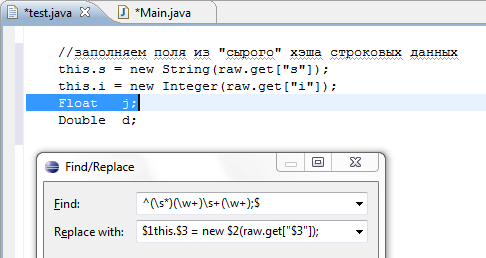
\includegraphics{fig/eclipseIde}
    \caption{Регулярные выражения в IDE Eclipse за работой}\label{fig:eclipseIde}
\end{figure} 

Регулярные выражения позволяют программисту уйти от написания собственных алгоритмов для решения рутинных задач специфичного поиска или замены в тексте, да и обычному пользователю они могут стать неплохим подспорьем при работе с данными в текстовом формате.


\section*{Задания}
\addcontentsline{toc}{section}{Задания}

\begin{enumerate}
    \item Сколько элементов в регулярном множестве, соответствующем регулярному PCRE выражению:
    \begin{enumerate}
        \item <<\textbackslash d\{3,4\}[a-z]\{2\}>>
        \item <<0x[0-9a-fA-F]\{1,8\}>>
        \item <<[0-7]\{1,8\}|(раз|два|три)(четыре|пять)>>
        \item <<\textbackslash d?\textbackslash d?\textbackslash d?>>
        \item <<\^{}\textbackslash b[a-f]\{1,4\}\textbackslash d?\textbackslash b\$>>
        \item <<0[0-7]\{1,7\}?>>
    \end{enumerate}

    \item Организовать в тексте поиск цепочек символов, представляющих собой корректное имя переменной во многих языках программирования: имя начинается с латинской буквы или знака подчеркивания, а заканчивается цепочкой произвольной длины, состоящей из латинских букв, цифр и знака подчеркивания. Имя переменной должно быть отделено от остального текста пустым пространством (пробелом, табуляцией, переносом строки).
    
    \item Организуйте в тексте поиск чисел. Примеры чисел: $0$, $-5$, $0.1$, $-2.24$, $-2.123e-15$, $-31.123E+7$. Запись числа $-31.123E+7$ называется \emph{научной нотацией} и её следует понимать так: $-31.123\cdot 10^{+7}$.
    
    \item Организуйте поиск адресов e-mail в тексте. Примеры адресов: <<kafevm@mail.ru>>, <<e.mail@dot.net.com>>, и т.д.
    
    \item Даты у разных народов пишутся по-разному. Например, в России принято писать сначала день, потом месяц, потом год: <<29.02.1982>>, <<29/02/1982>>. В США, например, даты пишут в таком порядке: месяц, день, год. Выполните замены американских дат российскими, учтя, что разделителями могут быть точка, дефис и косая черта. Числа, соответствующие дням и месяцам не обязательно дополняются ведущим нулем: <<1.1.2011>>. В тексте не встретится сокращенных записей для года (иногда пишут 82 вместо 1982).
    
    \item В базе данных скопилось множество номеров телефонов одного города. Пусть это будет Киров с международным кодом 8(8332). В свое время под номер была отведена строка, и операторы вводили номера телефонов, сообразуясь со своими эстетическими пристрастиями: 8-8332-123456, 8 8332 12 34 56, 8-8332-123-456, 8-8332-12-34-56, 8(8332)12 34 56. И даже без кода: 12 34 56, 123-456. Пора положить конец хаосу. Да будет единый: 8(8332)XX-XX-XX.
    
    \item Некоторая программа принимает на вход табличные данные (товар, цена, количество, ед.изм.) в формате CSV\footnote{}. В процессе их подготовки произошла ошибка и некоторые столбцы поменялись местами: (товар, количество, цена, ед.изм.). Используя регулярные выражения исправьте ошибку.
\begin{verbatim}
товар;   количество;цена;    ед_изм
Молоко;  10;        24.20;   бут.
Кефир;   15;        18.76;   пак.
Печенье; 5;         40.35;   кг.
Хлеб;    20;        24.20;   буханка
Яблоки;  5;         65.30;   кг.
Рельс;   1;         9999.99; шт.
\end{verbatim}
\end{enumerate}
 %Регулярные множества и выражения
    \chapter{Отношения и функции} 
\label{ch:rel:rel}
%rel: prefix
Отношения и функции являются важнейшими понятиями математики и активно используются для решения практических задач. Для углубленного изучения рекомендуются \cite{bib:sudoplatov:discrmath, bib:haggard:discrmathprogrammer}.


\section{Отношения}

При решении практических задач порой необходимо выбирать элементы, связанные некоторым соотношением.


\emph{$n$-местным отношением} или \emph{$n$-местным предикатом} $P$ на множествах $A_1, A_2, \ldots, A_n$ называется любое подмножество прямого произведения $A_1\times A_2\times \cdots\times A_n$.

Говорят, что элементы $x_1,x_2,\ldots,x_n$ (где $x_1\in A_1,x_2\in A_2,\ldots,x_n\in A_n$) связаны соотношением $P$ (обозначается $P(x_1,x_2,\ldots,x_n)$) тогда и только тогда, когда $(x_1,x_2,\ldots,x_n)\in P$.

\begin{itemize}
	\item При $n=1$ отношение называется \emph{унарным} или \emph{свойством}. 
	\item При $n=2$ отношение $P$ называется \emph{бинарным}. Если $P\subseteq A\times B$ и $(x,y)\in P$, то пишут также $x\,P\,y$. Примером бинарного отношения может являться отношение $\subseteq$.
	\item Отношение $P\subseteq A^n$ называют \emph{$n$-местным предикатом (отношением) на множестве $A$}. \emph{Двуместным (бинарным) отношением на множестве $\mathbb{R}$} является отношение $\leq$.
\end{itemize}


\section{Бинарные отношения}

Бинарные отношения нашли множество практических применений. Существует несколько способов задать бинарное отношение $P\subseteq A\times B$:
\begin{itemize}
    \item множеством упорядоченных пар из $A\times B$;
    \item точками в декартовой системе координат (где на осях будут отложены элементы $A$ и $B$);
    \item ориентированным графом, в котором вершинам будут соответствовать элементы $A\cup B$, а дугам элементы $(a,b)\in P$;
    \item матрицей смежности, строкам которой соответствуют элементы $A$, столбцам --- элементы $B$, а наличию (отсутствию) пары $(a,b)\in A\times B$ в отношении $P$ соответствует 1 (отсутствию --- 0) на пересечении соответствующих строки и столбца;
    \item перечислением множества смежных элементов: \[\{(a,C)|a\in A,C=\{b|(a,b)\in P\}\}.\]
\end{itemize}

\begin{exampl} Задача.
    На множестве 
        \[M=\{m_1,m_2,m_3,m_4,m_5,m_6\}\] 
    задано бинарное отношение $P\subseteq M\times M$:
    \begin{equation}
        \label{eq:binary}
        \begin{split}
            P=\{
                (m_1,m_2),
                (m_1,m_4),
                (m_2,m_3),
                (m_2,m_4),\\
                (m_2,m_6),
                (m_3,m_1),
                (m_3,m_4),
                (m_4,m_5),\\
                (m_4,m_6),
                (m_5,m_6),
                (m_6,m_1),
                (m_6,m_3)
            \}.
        \end{split}
    \end{equation}
    
    Задайте отношение различными способами.
\end{exampl}

\begin{proof}[Решение]
    Бинарное отношение \eqref{eq:binary} уже задано множеством пар из $M^2$. Представление в декартовой системе координат и ориентированным графом приведены на рисунках \ref{fig:binaryR} и \ref{fig:binaryRGraph} соответственно.
    
    \begin{figure}
        \centering
        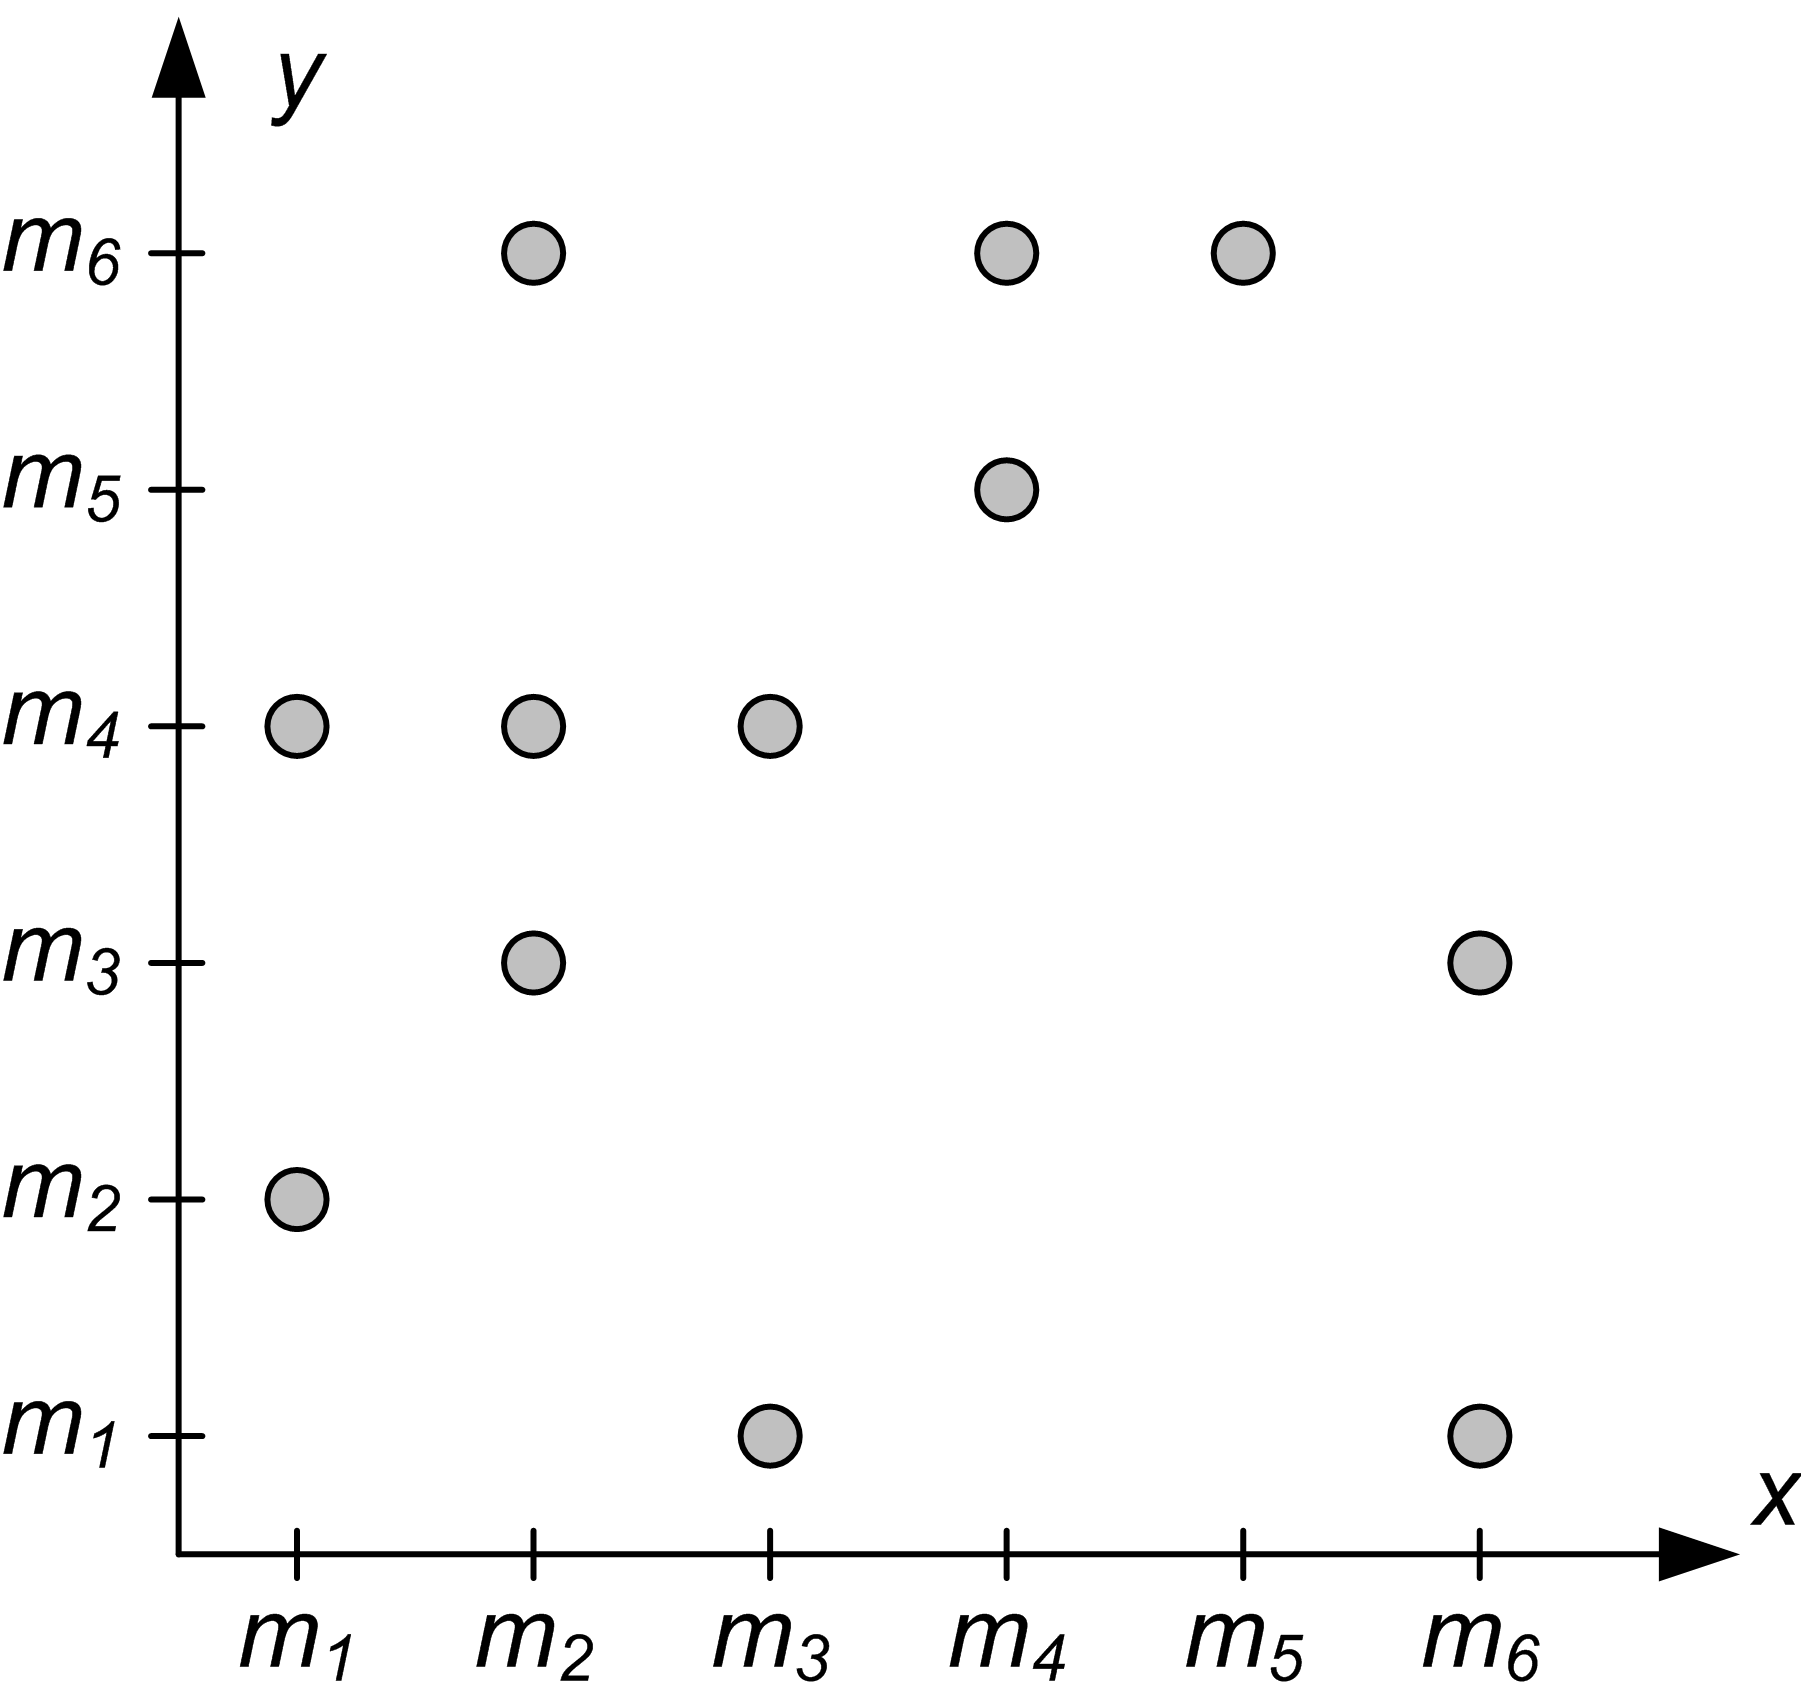
\includegraphics{fig/binaryR}
        \caption{Бинарное отношение в декартовой системе координат}
        \label{fig:binaryR}
    \end{figure} 

    \begin{figure}
        \[
            \xymatrix{
                *{}
                    &m_2 \ar@{->}[r]\ar@{->}[drr]\ar@{->}[dd]
                        &m_3 \ar@{->}[dll]\ar@{->}[dr]
                            &*{}
                                \\
                m_1 \ar@{->}[ur]\ar@{->}[rrr]
                    &*{}
                        &*{}
                            &m_4 \ar@{->}[dl]\ar@{->}[dll]
                                \\
                *{}
                    &m_6 \ar@{->}[ul]\ar@{->}[uur]
                        &m_5 \ar@{->}[l]
                            &*{}
            }
        \]
        \caption{Бинарное отношение задано орграфом}
        \label{fig:binaryRGraph}
    \end{figure} 

    Любое бинарное отношение $P=A\times B$ можно задать матрицей смежности $[P]$, по строкам которой расположены элементы множества $A$, по столбцам --- элементы $B$, а на пересечении строки $a$ и столбцa $b$ стоит 1, если $(a,b)\in P$ и 0 в противном случае. 

    Бинарное отношение \eqref{eq:binary} можно задать следующей \emph{матрицей смежности}\footnote{Договорившись о порядке следования строк и столбцов, шапку матрицы опускают}:

    \[
    [P]=
    \begin{array}{c|cccccc}
           &m_1&m_2&m_3&m_4&m_5&m_6\\ \hline
        m_1&0&1&0&1&0&0\\
        m_2&0&0&1&1&0&1\\
        m_3&1&0&0&1&0&0\\
        m_4&0&0&0&0&1&1\\
        m_5&0&0&0&0&0&1\\
        m_6&1&0&1&0&0&0
    \end{array}=
    \begin{pmatrix}
        0&1&0&1&0&0\\
        0&0&1&1&0&1\\
        1&0&0&1&0&0\\
        0&0&0&0&1&1\\
        0&0&0&0&0&1\\
        1&0&1&0&0&0
    \end{pmatrix}.
    \]

    Любое бинарное отношение $P\subseteq M^2$ можно задать также перечислением множества смежных элементов для каждого $x\in M$. Множество смежных с $x$ элементов определяется так: $\{y|(x,y)\in P\}$. 
    \[
        \begin{array}{c|l}
            \hline\hline
            x\in M&\{y|(x,y)\in P\}\\ \hline\hline
            m_1&\{m_2,m_4\}\\
            m_2&\{m_3,m_4,m_6\}\\
            m_3&\{m_1,m_4\}\\
            m_4&\{m_5,m_6\}\\
            m_5&\{m_6\}\\
            m_6&\{m_1,m_3\}\\ \hline
        \end{array}
    \]
    Бинарное отношение \eqref{eq:binary} будет задано перечислением множеств смежных вершин так:
    \[  
        \begin{split}
            \{
                (m_1,\{m_2,m_4\}), (m_2,\{m_3,m_4,m_6\}), (m_3,\{m_1,m_4\}),\\
                (m_4,\{m_5,m_6\}), (m_5,\{m_6\}),       (m_6,\{m_1,m_3\})\}.
        \end{split}
    \]
\end{proof}

Важными частными случаями \emph{бинарного} отношения на множестве $A$ являются:
\begin{itemize}
    \item \emph{тождественное} отношение (или \emph{диагональ}): $I_A=\{(a,a)|a\in A\}$;
    \item \emph{универсальное} (или \emph{полное}) отношение: $U_A=A^2$.
\end{itemize}

Для бинарного отношения $P$.
\begin{itemize}
    \item \emph{Областью определения} называется множество $\delta_P=\{a|(a,b)\in P\}$.
    \item \emph{Областью значений} называется множество $\rho_P=\{b|(a,b)\in P\}$.
\end{itemize}

\emph{Обратным} к $P$ отношением называется отношение
\[P^{-1}=\{(b,a)|(a,b)\in P\}.\]

\emph{Дополнением} отношения $P\subseteq A\times B$ называется отношение
\[\overline{P}=\{(a,b)|(a,b)\in A\times B\land (a,b)\not\in P\}.\]


\subsection{Композиция и возведение в степень}

Вводится понятие \emph{композиции} (\emph{произведения}) отношений $P_1\subseteq A\times B$ и $P_2\subseteq B\times C$:
\begin{equation}
    \label{eq:binPComposition}
    \begin{split}
        P_1\cdot P_2 = P_1P_2 = \\
        = \{(a,c)|a\in A\land c\in C\land (\exists b\in B (a,b)\in P_1\land (b,c)\in P_2)\}
    \end{split}
\end{equation}

\begin{exampl} Задача. 
    \label{exampl:binPComposition}
    Дано три множества $A=\{g,h\}$, $B=\{1,2,3\}$, $C=\{s,t\}$. Заданы отношения $P\subseteq A\times B$, $Q=B\times C$: 
    \[P=\{(g,1),(g,2),(g,3),(h,2)\},Q=\{(1,t),(2,s),(3,s)\}.\]
\end{exampl}

\begin{proof}[Решение]
    Построим орграф, соответствующий композиции $PQ$. Оба отношения можно задать на одном орграфе:
    \[
    \xymatrix{
        g  \ar@{->}[rr] \ar@{->}[drr] \ar@{->}[ddrr]
            &*{}
                &1 \ar@{->}[ddrr]
                    &*{}
                        &s 
                            \\
        *{}
            &*{}
                &2 \ar@{->}[urr]
                    &*{}
                        &*{}
                            \\
        h \ar@{->}[urr]
            &*{}
                &3 \ar@{->}[uurr]
                    &*{}
                        &t
                            \\
        *{}
            &*{P}
                &*{}
                    &*{Q}
                        &*{}
    }
    \]

    Выполняя композицию:
    \[
        \begin{array}{cc}
        {
            \raisebox{-0.5\height}{
            \(
                \begin{array}{l}
                    g\,P\,1\land 1\,Q\,t\Rightarrow (g,t)\in PQ\\
                    g\,P\,2\land 2\,Q\,s\Rightarrow (g,s)\in PQ\\
                    g\,P\,3\land 3\,Q\,s\Rightarrow (g,s)\in PQ\\
                    h\,P\,2\land 2\,Q\,s\Rightarrow (h,s)\in PQ\\
                    \\
                    PQ=\{(g,t),(g,s),(h,s)\}
                \end{array}
            \)
            }
        }
        &
        {\xymatrix{
                g  \ar@{->}[rr] \ar@{->}[drr]
                    &*{}
                        &s
                            \\
                h \ar@{->}[urr]
                    &*{}
                        &t 
                            \\
                *{}
                    &*{PQ}
                        &*{}
        }}
        \end{array}
    \]
    
    Получим ответ $PQ=\{(g,t),(g,s),(h,s)\}$.
\end{proof}

Для бинарного отношения $P$ на $A$ вводится понятие возведения в степень:
\[
    P^n=
    \begin{cases}
        P^{0}=I_A,\,n=0;\\
        P^{n}=P^{n-1}\cdot P,\,n>0.
    \end{cases}
\]
т.е.
\[
    P^n=\underbrace{P\cdot P\cdot\cdots P}_n.
\]


\subsection{Операции на матрицах смежности}

Пусть $A=\{a_1,\ldots,a_m\}$, $B=\{b_1,\ldots,b_n\}$, $C=\{c_1,\ldots,c_k\}$ и бинарные отношения $P\subseteq A\times B$, $Q=B\times C$ заданы матрицами смежности $[P]_{m\times n}$ и $[Q]_{n\times k}$.

Матрица их композиции $[PQ]_{m\times k}$ называется \emph{логическим} или \emph{булевым} произведением матриц исходных отношений $[P]_{m\times n}\cdot [Q]_{n\times k}$.

Каждый элемент матрицы композиции получается по формуле
\[
    [PQ]_{i,j}=\bigvee_{l=1}^{n} [P]_{i,l}\land [Q]_{l,j},
    1\leq i\leq m, 1\leq j\leq k,
\]
где $\bigvee$ обозначает групповое логическое <<ИЛИ>>.

\begin{exampl}
    \label{exampl:binPcompositionMatrix}
    Для отношений из примера \ref{exampl:binPComposition} матрицы смежности:
    \[
        [P]_{2\times 3}=
        \begin{array}{c|ccc}
              & 1 & 2 & 3 \\ \hline
            g & 1 & 1 & 1 \\
            h & 0 & 1 & 0
        \end{array}=
        \begin{pmatrix}
            1&1&1\\
            0&1&0
        \end{pmatrix},\,
        [Q]_{3\times 2}=
        \begin{array}{c|cc}
              & s & t \\ \hline
            1 & 0 & 1 \\
            2 & 1 & 0 \\
            3 & 1 & 0 
        \end{array}=
        \begin{pmatrix}
            0&1\\
            1&0\\
            1&0
        \end{pmatrix}.
    \]

    И матрица композиции:
    \[
        [PQ]_{2\times 2}=
        [P]_{2\times 3}\cdot [Q]_{3\times 2}=
        \begin{pmatrix}
            1&1&1\\
            0&1&0
        \end{pmatrix}\cdot
        \begin{pmatrix}
            0&1\\
            1&0\\
            1&0
        \end{pmatrix}=
        \begin{pmatrix}
            1&1\\
            1&0
        \end{pmatrix}=
        \begin{array}{c|ccc}
              & s & t \\ \hline
            g & 1 & 1 \\
            h & 1 & 0 
        \end{array}.
    \]

    Например, элемент $[PQ]_{2,2}$ получается так:
    \[
    [PQ]_{2,2}=\begin{pmatrix}0&1&0\end{pmatrix}\cdot\begin{pmatrix}1\\0\\0\end{pmatrix}=
    (0\land 1)\lor(1\land0)\lor(0\land 0)=0\lor 0\lor 0 = 0.
    \]
    \qed
\end{exampl}

Если оба бинарных отношения $P,Q\subset A\times B$ заданы матрицами смежности $[P]_{m\times n}$ и $[Q]_{m\times n}$, то:
\begin{itemize}
    \item элементы матрицы объединения отношений
    \[
        [P\cup Q]_{i,j}=[P]_{i,j}\lor [Q]_{i,j};
    \]
    
    \item элементы матрицы пересечения отношений
    \[
        [P\cap Q]_{i,j}=[P]_{i,j}\land [Q]_{i,j}.
    \]
\end{itemize}

Матрица \emph{обратного} к $P$ отношения представляет собой транспонированную матрицу отношения $P$:
\[
    [P^{-1}]_{n\times m}=([P]_{m\times n}])^{T}, 
\]
где каждый элемент $[P^{-1}]_{i,j}=[P]_{j,i}, 1\leq j\leq m, 1\leq i\leq n.$

Матрица \emph{дополнения} $P$:
\[
    [\overline{P}]_{i,j}=\overline{ [P]_{i,j} }.
\]

\begin{exampl}
    Рассмотрим матричную реализацию основных операций на отношениях из примера \ref{exampl:binPComposition}. Введем дополнительно\footnote{Лишь для того, чтобы получить отношение $R$. Отношение $P$ и $Q^{-1}$, несмотря на одинаковую размерность матриц, объединять, очевидно, нельзя.} отношение $S\subseteq A\times C$:
    \[
        [S]_{2\times 2}=
        \begin{array}{c|cc}
              & s & t \\ \hline
            g & 1 & 0 \\
            h & 0 & 1 
        \end{array}=
        \begin{pmatrix}
            1&0\\
            0&1
        \end{pmatrix}.        
    \]
    И определим $R\subseteq A\times B$:
    \[
        [R]=[S]\cdot[Q^{-1}]=
        [S]\cdot[Q]^T=
        \begin{array}{c|ccc}
              & 1 & 2 & 3 \\ \hline
            g & 0 & 1 & 1 \\
            h & 1 & 0 & 0
        \end{array}=
        \begin{pmatrix}
            0 & 1 & 1 \\
            1 & 0 & 0
        \end{pmatrix}.        
    \]
    Тогда:
    \[
    \begin{split}
    [P\cup R]=[P]\lor[R]=
        \begin{pmatrix}1&1&1\\0&1&0\end{pmatrix}\lor
        \begin{pmatrix}0&1&1\\1&0&0\end{pmatrix}=
        \begin{pmatrix}1&1&1\\1&1&0\end{pmatrix},\\
    [P\cap R]=[P]\land[R]=
        \begin{pmatrix}1&1&1\\0&1&0\end{pmatrix}\land
        \begin{pmatrix}0&1&1\\1&0&0\end{pmatrix}=
        \begin{pmatrix}0&1&1\\0&0&0\end{pmatrix}.
    \end{split}    
    \]
    \qed
\end{exampl}


\section{Функции}

Отношение $f\subseteq A\times B$ называется \emph{функцией} или \emph{отображением} из множества $A$ в множество $B$, если область определения $\delta_f=A$, область значений $\rho_f\subseteq B$ и из $(x_1,y_1)\in f$, $(x_2,y_2)\in f$ следует $y_1=y_2$. Если вместо $\delta_f=A$ выполняется $\delta_f\subset A$, то $f$ называется \emph{частичной} функцией.

\[
    \begin{array}{c|c}
        \begin{array}{c}
            {
                \xymatrix{
                    x_1  \ar@{->}[r] \ar@{->}[dr]
                        &y_1
                            \\
                    x_2 \ar@{->}[r]
                        &y_2 
                            \\
                    x_3 \ar@{->}[r]
                        &y_3
                }
            }\\
            \text{Отношение, но не функция!}
        \end{array}
        &
        \begin{array}{c}
            {
                \xymatrix{
                    x_1  \ar@{->}[r]
                        &y_1
                            \\
                    x_2 \ar@{->}[dr]
                        &y_2 
                            \\
                    x_3 
                        &y_3
                }    
            }\\
            \text{Частичная функция}
        \end{array}
    \end{array}
\]

Функция из $A$ в $B$ обозначается так:
\[f:A\to B.\]

Если $(x,y)\in f$, то пишем $y=f(x)$ или $f:x\mapsto y$ (читаем как <<функция $f$ ставит в соответствие элементу $x$ элемент $y$>>).

Функция $f:A\to B$ называется \emph{разнозначной}, функцией $A$ в $B$ или \emph{инъекцией}, если $f^{-1}$ --- \emph{частичная} функция. То есть справедливо, что для любых двух элементов из области определения $x_1,x_2\in\delta_f$ из $x_1\neq x_2$ следует $f(x_1)\neq f(x_2)$. Обозначают инъекцию $f:A\xrightarrow{\text{в}} B$.

Функция $f:A\to B$ называется функцией $A$ на $B$ или \emph{сюръекцией} если область значений $\rho_f=B$. Обозначают сюръекцию $f:A\xrightarrow{\text{на}} B$.

\[
    \begin{array}{c|c|c}
        \begin{array}{c}
            {
                \xymatrix{
                    x_1  \ar@{->}[r]
                        &y_1
                            \\
                    x_2 \ar@{->}[dr]
                        &y_2 
                            \\
                    *{}
                        &y_3
                }
            }\\
            \text{Инъекция}\\
            f:X\xrightarrow{\text{в}} Y\\
            \text{Не сюръекция!}
        \end{array}
        &
        \begin{array}{c}
            {
                \xymatrix{
                    x_1  \ar@{->}[r]
                        &y_1
                            \\
                    x_2 \ar@{->}[r]
                        &y_2 
                            \\
                    x_3 \ar@{->}[ur]
                        &*{}
                }    
            }\\
            \text{Сюръекция}\\
            f:X\xrightarrow{\text{на}} Y\\
            \text{Не инъекция!}
        \end{array}
        &
        \begin{array}{c}
            {
                \xymatrix{
                    x_1 \ar@{->}[r]
                        &y_1
                            \\
                    x_2 \ar@{->}[ur]
                        &y_2 
                            \\
                    x_3 \ar@{->}[ur]
                        &y_3
                }    
            }\\
            f:X\to Y\\
            \text{Не сюръекция!}\\
            \text{Не инъекция!}
        \end{array}        
    \end{array}
\]

Функция $f$ называется \emph{взаимно однозначным соответствием} между множествами $A$ и $B$ или \emph{биекцией}, если она является одновременно и инъекцией и сюръекцией. Обозначают биекцию так: $f:A\leftrightarrow B$. 
\[
    \begin{array}{c}
        {
            \xymatrix{
                x_1  \ar@{->}[r]
                    &y_1
                        \\
                x_2 \ar@{->}[dr]
                    &y_2 
                        \\
                x_3 \ar@{->}[ur]
                    &y_3
            }
        }\\
        \text{Биекция} f:X\leftrightarrow Y\\
        \text{Cюръекция и инъекция одновременно!}
    \end{array}
\]

Биекцию $f:A\leftrightarrow A$ называют \emph{подстановкой} множества $A$.

В отношении функций на рисунке \ref{fig:functionProps}.
\begin{itemize}
    \item $f_1$ на данной области определения не является \emph{функцией}! Это \emph{частичная} функция.
    \item $f_2$ \emph{сюръективна}, но \emph{не инъективна}.
    \item $f_3$ \emph{биективна} (стало быть и \emph{инъективна} и \emph{сюръективна}).
    \item $f_4$ \emph{инъективна}, но \emph{не сюръективна}.
    \item $f_5$ \emph{не инъективна} и \emph{не сюръективна}.
\end{itemize}

\begin{figure}
    \centering
    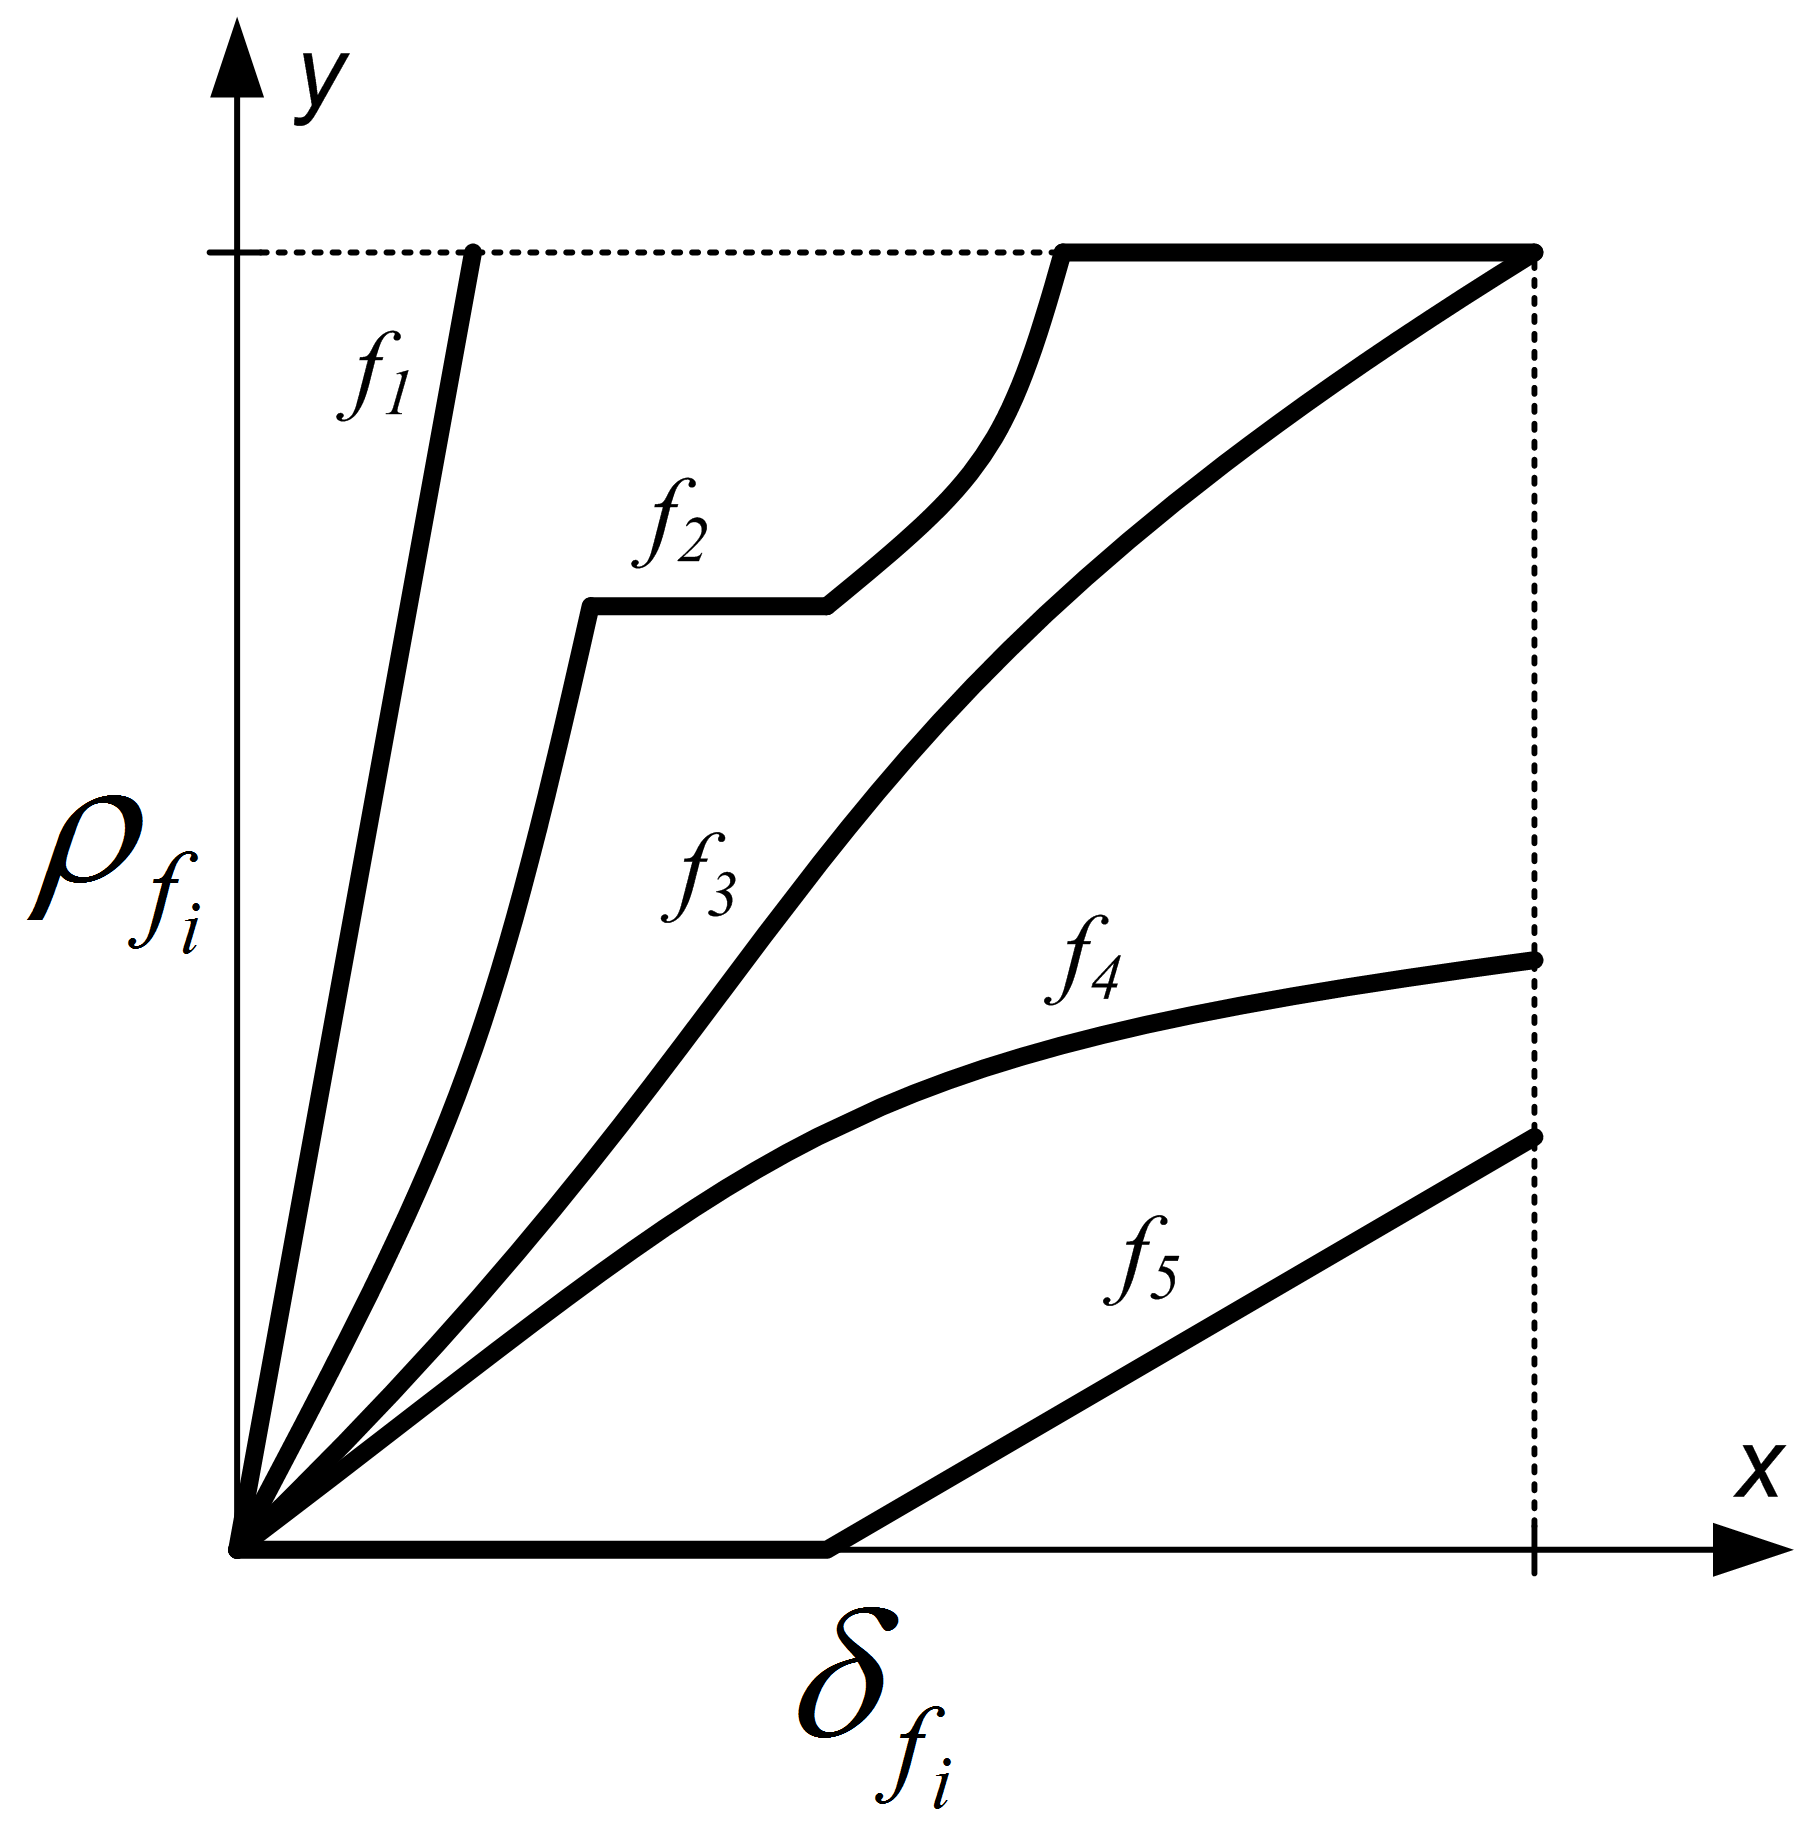
\includegraphics{fig/functionProps}
    \caption{Функции}\label{fig:functionProps}
\end{figure} 

\begin{itemize}
    \item Функция $f:\mathbb{N}\to B$ называется \emph{последовательностью}.

    \item Функция $f:A^n\to B$ называется \emph{$n$-местной функцией} из $A$ в $B$. 

    \item Функция $f:A^n\to A$ называется \emph{$n$-местной алгебраической операцией} на множестве $A$. При $n=1$ операция называется \emph{унарной}, при $n=2$ --- \emph{бинарной}, в остальных случаях --- $n$-арной. При $n=0$ операция $f:A^0\to A$ есть множество $\{(\emptyset,a)\}$ для некоторого $a\in A$. В этом случае операцию обычно называют \emph{константой} и отождествляют с $a$.
\end{itemize}


\section*{Задания}
\addcontentsline{toc}{section}{Задания}

\begin{enumerate}
    \item Задайте матрицу смежности бинарного отношения $\subseteq$ на элементах множества $2^M$, где $M=\{a,b,c\}$.

    \item Задать бинарное отношение $P$ орграфом, матрицей смежности и перечислением пар.
    \begin{enumerate}
        \item  $P\subset A\times B$, $A=\{1,3,5,7\}$, $B=\{2,4,6\}$, $P=\{(a,b)|a+b=9\}$.
        \item  $P\subset A\times B$, $A=\{1,3,5,7\}$, $B=\{2,4,6\}$, $P=\{(a,b)|a<b\}$.
    
        \item $P\subset A^2$, $A=\{1,2,3,4\}$, $P=\{(a,b)|a+2b\equiv 1\pmod{2}\}$.
        \item $P\subset \mathbb{N}^2$, $P=\{(a,b)|2a+b=9,a\neq 0\}$.
        \item $P\subset \mathbb{N}^2$, $P=\{(a,b)|a+b<5\}$.
        
        \item $P\subset \mathbb{N}^2$, $P=\{(x,y)|(x^2=y)\land (0\leq y\leq 100)\}$.
        \item $P\subset \mathbb{N}^2$, $P=\{(x,y)|(x\cdot z^2=y)\land (z\in\mathbb{N})\land (0\leq y\leq 100)\}$.        
    \end{enumerate}
    
    
    \item Задать отношение <<возможен ход с клетки $c_1$ на клетку $c_2$>> (определив множество пар координат с помощью характеристического предиката) клеток шахматной доски (их координат) $c_1=(x_1,y_1)$ и $c_2=(x_2,y_2)$ для следующей шахматной фигуры:
    \begin{enumerate}
        \item пешка;
        \item офицер;
        \item ладья;
        \item конь;
        \item король;
        \item ферзь.
    \end{enumerate}
    
    \item Даны два отношения $P=\{(0,1),(1,2),(2,3),(0,4),(1,5),(2,0)\}$ и $Q=\{(0,0),(1,1),(2,0),(3,1),(4,0),(5,1)\}$. Представить каждое матрицей смежности, найти отношение $PQ$ и построить соответствующий ему орграф.
    
    
    \item Бинарное отношение $P$ на множестве $A=\{1,2,3,4\}$ задано графом.
    \[
        \begin{array}{c}
            {
                \xymatrix{
                    1
                        &2 \ar@{->}[l]
                            \\
                    4 \ar@{->}[r]
                        &3 \ar@{->}[u]
                }    
            }\\
            P
        \end{array}
    \]
    
    Необходимо задать его аналитическим описанием, перечислением пар и матрицей смежности.
    
    
    \item Два бинарных отношения $P$ и $Q$ на множестве $\{0,1,2,3\}$ заданы графами. Определить, проведя вычисления на матрицах смежности, графы отношений $PQ$ и $QP$.
    \[
        \begin{array}{cc}
            \begin{array}{c}
                {
                    \xymatrix{
                        0  \ar@{->}[r]
                            &1 \ar@{->}[d]
                                \\
                        3 \ar@{->}[u]
                            &2 \ar@{->}[l]
                    }    
                }\\
                P
            \end{array}
            &
            \begin{array}{c}
                {
                    \xymatrix{
                        0  \ar@{->}[dr]
                            &1 \ar@{->}[l]
                                \\
                        3 \ar@{->}[ur]
                            &2 \ar@{->}[l]
                    }    
                }\\
                Q
            \end{array}
        \end{array}
    \]

    \item В модулярной арифметике все вычисления происходят <<по фиксированному модулю>> $p$. Т.е. все натуральные аргументы операций изменяются в пределах от $0$ до $p-1$ а результат получается как остаток от деления на $p$. Например: $4+3\equiv 2\pmod{5}$. Далее приведен граф $P$ унарной операции \emph{инкремент} по модулю 5.
    \[
        \begin{array}{c}
            {\xymatrix{
                *{}  
                    &*{} 
                        &1  \ar@{->}[drr]
                            &*{} 
                                &*{}  
                                    \\
                0  \ar@{->}[urr]
                    &*{}  
                        &*{}  
                            &*{}  
                                &2  \ar@{->}[dl]
                                    \\
                *{}  
                    &4  \ar@{->}[ul]
                        &*{}  
                            &3  \ar@{->}[ll]
                                &*{}  
            }}\\
            P
        \end{array}
    \]
    Найти $P^2,P^3,P^4,P^5$ и объяснить словесно, какой унарной операции эти степени инкремента соответствуют.
    
    \item Доказать, что для бинарных отношений $P,Q$ справедливо:
    \begin{enumerate}
        \item $(P^{-1})^{-1}=P$;
        \item $(P\cdot Q)^{-1}=Q^{-1}\cdot P^{-1}$;
        \item $(P\cdot Q)\cdot R=P\cdot(Q\cdot R)$;
        \item $P\cdot Q\neq Q\cdot P$.
    \end{enumerate}
    
    \item Пусть $f(x)=x^2+2x+2$ и $g(x)=\sin(x)$. Найти:
    \begin{enumerate}
        \item $(f\cdot g)(x)$;
        \item $(g\cdot f)(x)$;
        \item $(g\cdot f^{-1})(x)$;
        \item $(f^{-1}\cdot g)(x)$;
    \end{enumerate}
    
    \item Какими свойствами (инъективности, сюръективности, биективности) обладает функция $f:\mathbb{R}\to\mathbb{R}$:
    \begin{enumerate}
        \item $f(x)=e^x$;
        \item $f(x)=x\cdot \sin{(x)}$;
        \item $f(x)=2x-1$;
        \item $f(x)=x^2-1$;
        \item $f(x)=x^3-1$;
        \item $f(x)=2x^3-3x^2+1$.
    \end{enumerate}
    
    Привести примеры частичных функций $f$.
    
    \item Доказать, что:
    \begin{enumerate}
        \item если $f:A\to B$ и $g:B\to C$, то $f\cdot g:A\to C$;
        
        \item если $f:A\xrightarrow{\text{на}} B$ и $g:B\xrightarrow{\text{на}} C$, то $f\cdot g:A\xrightarrow{\text{на}} C$;
        
        \item если $f:A\xrightarrow{\text{в}} B$ и $g:B\xrightarrow{\text{в}} C$, то $f\cdot g:A\xrightarrow{\text{в}} C$;
        
        \item если $f:A\leftrightarrow B$ и $g:B\leftrightarrow C$, то $f\cdot g:A\leftrightarrow C$;
        
        \item если $f:A\leftrightarrow B$, то $f^{-1}:B\leftrightarrow A$, то $f\cdot f^{-1}=I_A$ и $f^{-1}\cdot f=I_B$.
    \end{enumerate}

    \item Очень важным элементом в системах пакетной передачи данных является коммутатор --- устройство, позволяющее передавать пакеты информации в нужные каналы. При этом пакет информации содержит <<адрес>> канала назначения в служебных полях. Каждый элемент $i$-го слоя коммутационной сети (см. рис. \ref{fig:rel:commutate}) автономен и работает так: получив пакет (пакеты поступают на входы $a,b$), элемент просматривает $i$-й бит адреса $a_i$ канала назначения и направляет пакет на выход $c$, если $a_i=0$, или на выход $d$, если $a_i=1$. 
    
    На рисунке \ref{fig:rel:commutate} приведена коммутационная сеть на восемь входов и восемь выходов, состоящая из трех четырехэлементных слоёв. Задав для каждого слоя отношение <<вход $x$ может поступать на выход $y$>> и функции перестановки для соседних слоев <<i-й выход слоя поступает на j-й вход следующиго слоя>>, формально докажите, что пакет, поступивший на любой вход первого слоя может выйти на любой выход третьего.

    \begin{figure}
        \centering
        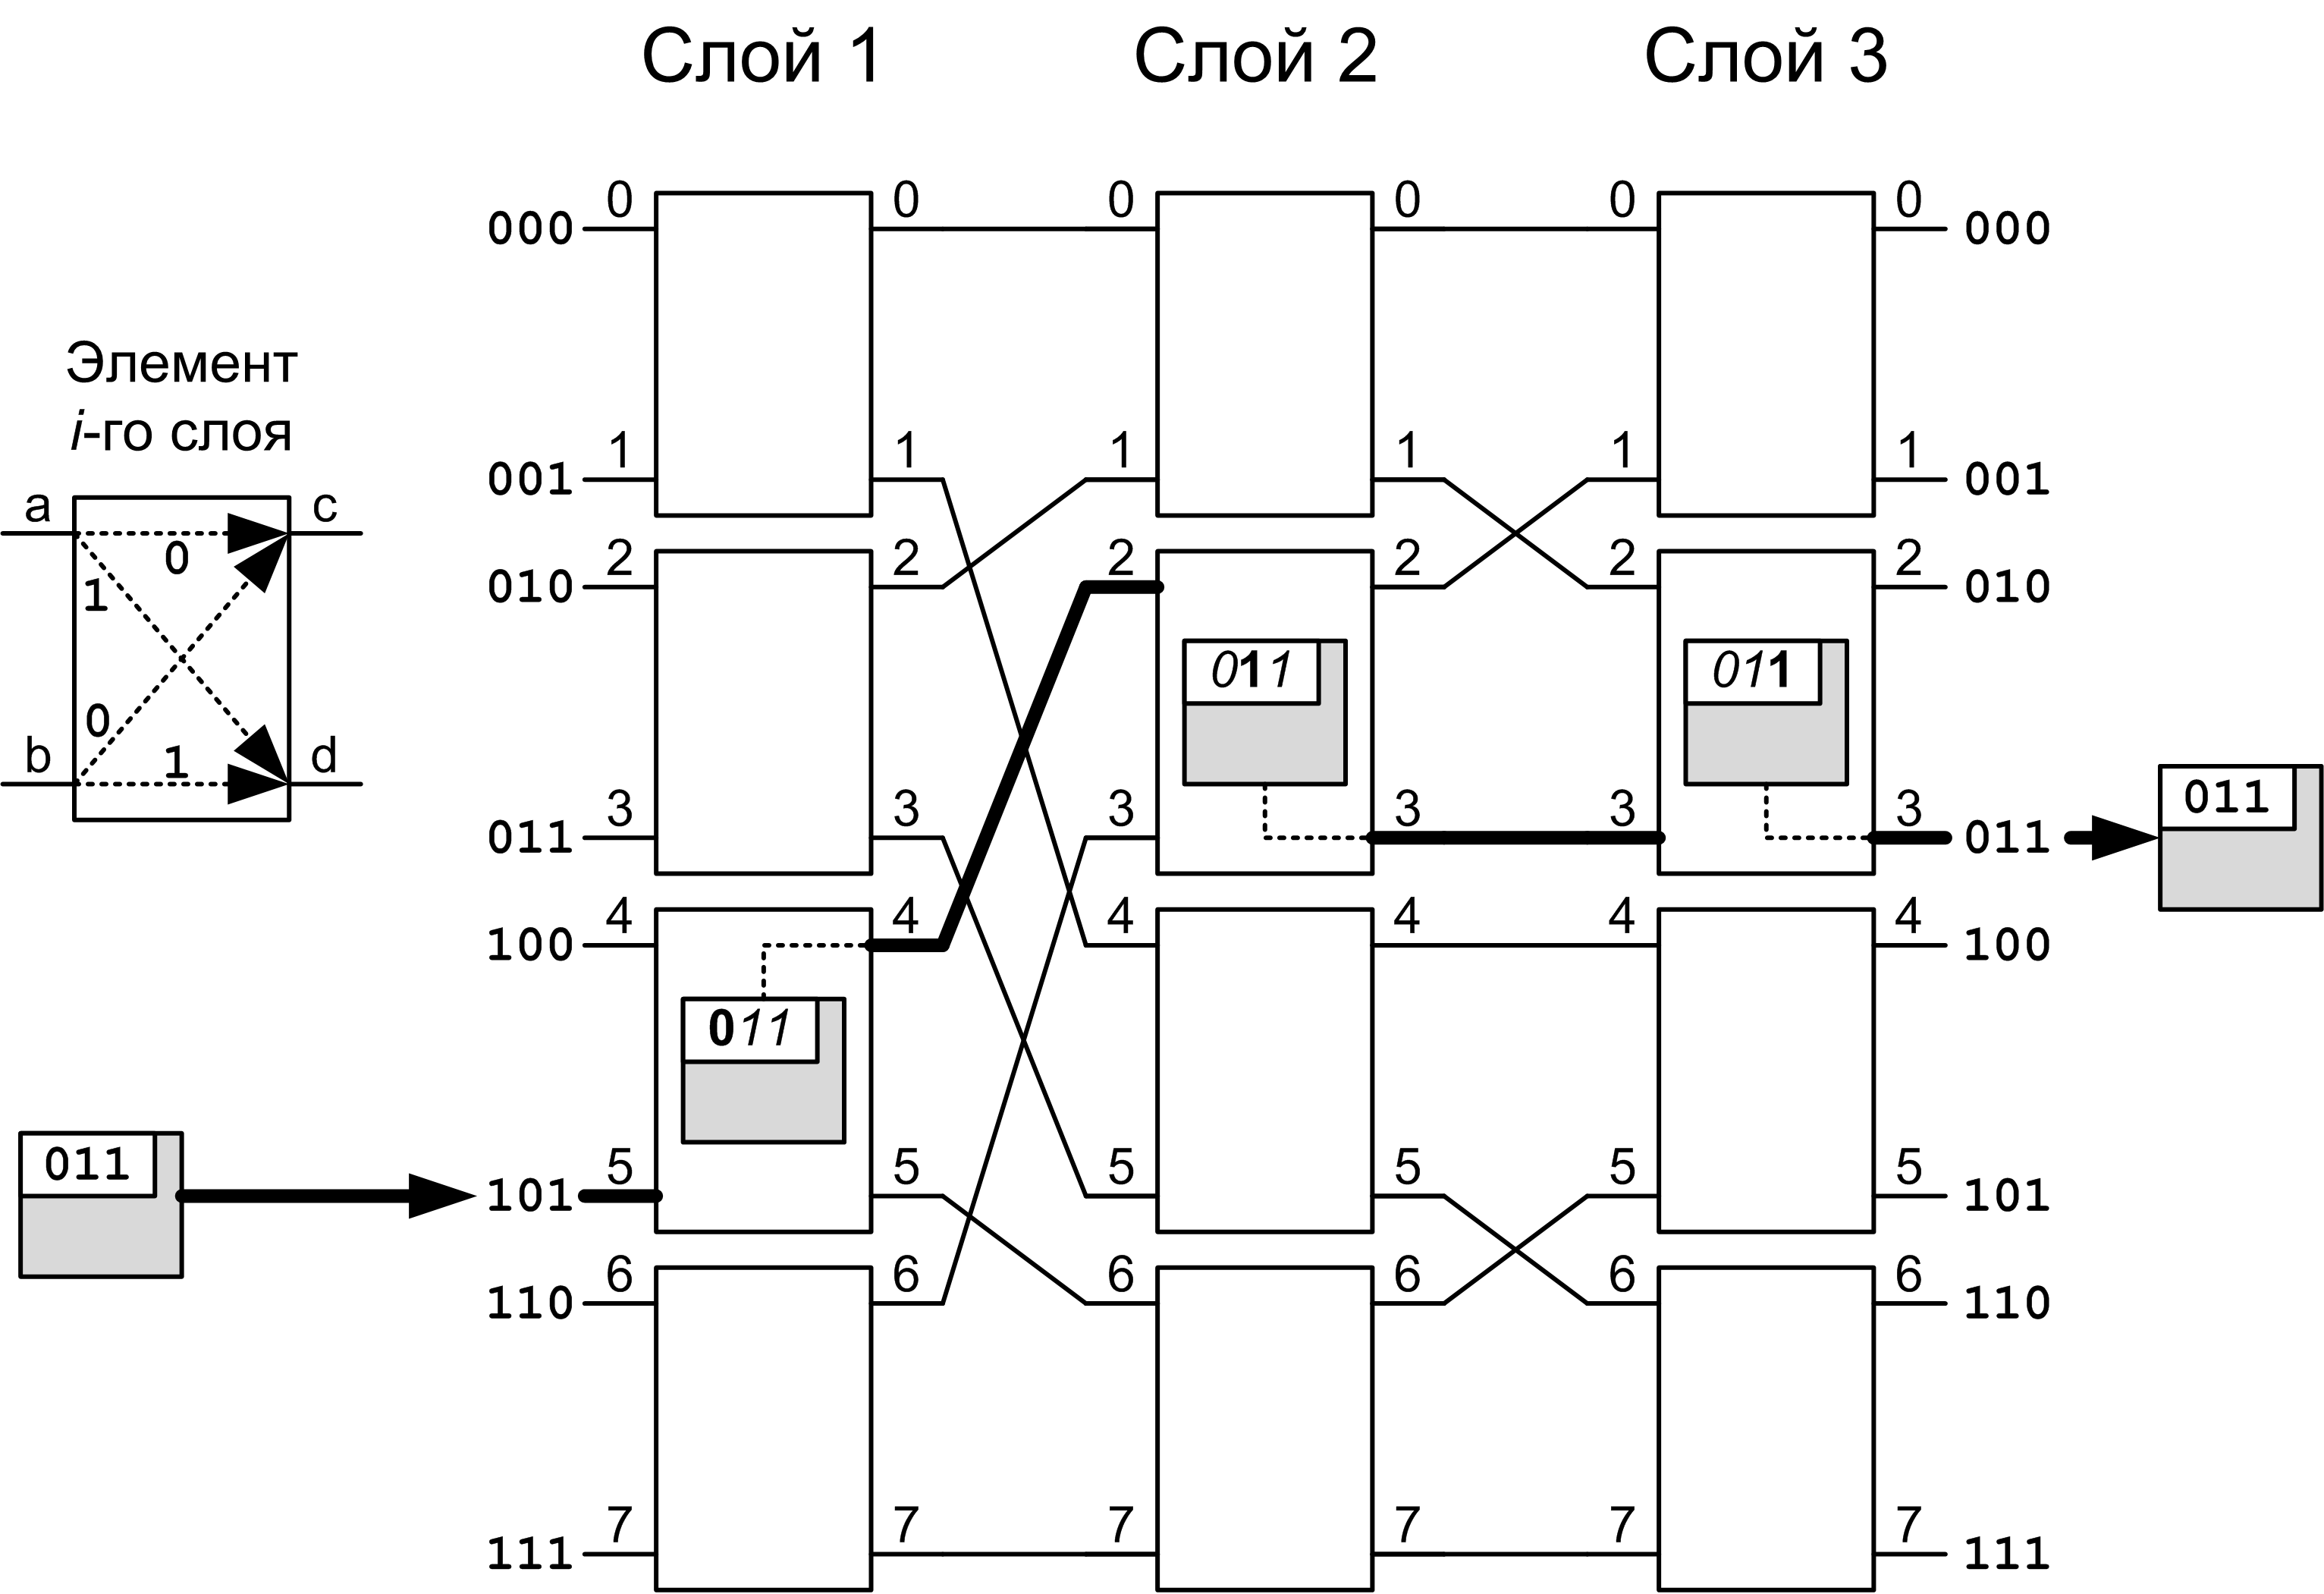
\includegraphics[width=0.7\textwidth]{fig/commutate}
        \caption{Сеть коммутации $8\times 8$}
        \label{fig:rel:commutate}
    \end{figure} 
    
\end{enumerate}
 %Отношения и функции
    \chapter{Мощность множества}

%pwr: prefix
Дается более строгое определение мощности. Для углубленного изучения рекомендуются \cite{bib:sudoplatov:discrmath,bib:shaporev:discretemath}.


\section{Основные теоремы и определения}

Множества $A$ и $B$ называются \emph{эквивалентными} (обозначается $A\sim B$), если существует биекция $f:A\leftrightarrow B$.

\begin{enumerate}
	\item $A\sim A$ (так как существует $I_A:A\leftrightarrow A$);
	\item Если $A\sim B$, то $B\sim A$ (так как существует $f:A\leftrightarrow B$, то существует и $f^{-1}:B\leftrightarrow A$);
	\item Если $A\sim B$ и $B\sim C$, то $A\sim C$ (так как из $f:A\leftrightarrow B$ и $g:B\leftrightarrow C$ следует $f\cdot g:A\leftrightarrow C$).	
\end{enumerate}

\emph{Мощностью} множества $A$ называется класс всех множеств, эквивалентных множеству $A$ (обозначается $|A|$). Эквивалентные множества $A$ и $B$ называются \emph{равномощными} $|A|=|B|$.

Если $A\sim \{0,1,\ldots,n-1\}$ для некоторого $n\in\mathbb{N}$, т.е. $A$ имеет ровно $n$ элементов, то множество $A$ называется \emph{конечным}. В этом случае пишут $|A|=n$. Мощностью конечного множества является количество входящих в него элементов.

Множество, не являющееся конечным, называется \emph{бесконечным}. В бесконечном 
множестве $A$ всегда найдется подмножество $B$, эквивалентное ему: $\exists B\subset A\land B\sim A$, причем разность $A\backslash B$ есть бесконечное множество. Это, пожалуй, основной признак, по которому можно отличить конечное множество от бесконечного.

Если $A\sim \mathbb{N}$, то $A$ называется \emph{счетным}: $|A|=\aleph_0$. Всякое бесконечное множество $A$ содержит счетное множество $B$, причем такое, что $A\backslash B$ есть бесконечное множество.

\begin{exampl}
    Множества $\mathbb{Z}$ и $\mathbb{N}$ \emph{равномощны}.
\end{exampl}
\begin{proof}
    Построим функцию $f:\mathbb{N}\leftrightarrow\mathbb{Z}$:
    \[
        f(n)=
        \begin{cases}
             i,     &\text{если $n=2\cdot i,i\in\mathbb{N}$}\\
            -(i+1), &\text{если $n=2\cdot i+1,i\in\mathbb{N}$}
        \end{cases}
    \]
    Видно, что 
    \[
        f=\{0\mapsto 0,1\mapsto -1,2\mapsto 1,3\mapsto -2,4\mapsto 2,5\mapsto-3,6\mapsto 3,\ldots\}
    \]
\end{proof}

\begin{exampl}
    Множество всех цепочек, состоящих из символов конечного алфавита $T$ счетно\footnote{Да, слова из словаря русского языка можно взаимооднозначно пронумеровать!}.
\end{exampl}
\begin{proof}
    Пусть $T=\{s_1,s_2,\ldots,s_n\}$. Построим отображение на подмножество множества натуральных чисел $\mathbb{N}$ и будем в качестве алфавита рассматривать $T'=\{0,1,\ldots,n-1\}$. Тогда любую цепочку $c=b_mb_{m-1}\cdots b_0$, где $b_i\in T'$ можно рассматривать как целое число $X$ в $n$-ичной системе счисления:
    \[
        X=b_m\cdot n^m + b_{m-1}\cdot n^{m-1} + \cdots + b_1\cdot n + b_0.
    \]
\end{proof}

Говорят, что мощность множества $A$ \emph{не превосходит} мощности множества $B$ ($|A|\leq|B|$), если $A$ эквивалентно некоторому подмножеству множества $B$. Мощность множества $A$ \emph{меньше} мощности множества $B$ ($|A|<|B|$), если $|A|\leq|B|$ и $|A|\neq|B|$.

\begin{Theor}[Кантора-Бернштейна] 
\label{Theor:KantorBernstain}
Если из двух множеств $A$ и $B$ каждое эквивалентно части другого, то эти множества эквивалентны между собой. Т.е. если $|A|\leq|B|$ и $|B|\leq|A|$, $|A|=|B|$.
\end{Theor}
\begin{proof}
	Так как $A\sim B_1$, где $B_1\subseteq B$, то найдется функция $f$, такая, что $f:A\leftrightarrow B_1$, а значит $f:A\xrightarrow{\text{в}}B$. Аналогично найдется $g:B\xrightarrow{\text{в}}A$, так как $B\sim A_1$, где $A_1\subseteq A$. См. рис. \ref{fig:kantorBernstein1}.

	Пусть $A_0=A$, $A_1=g(B)$, $A_{n+2}=(f\cdot g)(A_n)$. Видно, что $A_{n+1}\subseteq A_n$. Пусть $M_i=A_i\backslash A_{i+1}$. Видно, что существует биекция $f\cdot g:M_{i}\leftrightarrow M_{i+2}$ см. рис. \ref{fig:kantorBernstein2}. Справедливо также, что при $i\neq j$ выполняется $M_i\cap M_j=\emptyset$. Обозначим $D=\bigcap_{k\in\mathbb{N}} A_k$. 

	Очевидно, что $A_k=(\bigcup_{i\in\mathbb{N},i\geq k}M_i)\cup D$. Определим (см. рис. \ref{fig:kantorBernstein3}) биективное отображение $h:A\leftrightarrow A_1$:
	\[
	h(a)=
		\begin{cases}
			a,             &\text{если\,} a\in(\bigcup_{i\in\mathbb{N}}M_{2i+1})\cup D\\
			(f\cdot g)(a), &\text{если\,} a\in\bigcup_{i\in\mathbb{N}}M_{2i}.
		\end{cases}
	\]

	Раз оно существует, то $A\sim A_1$, но и $B\sim A_1$, следовательно $A\sim B$, то есть $|A|=|B|$.
\end{proof}

\begin{figure}
    \centering
    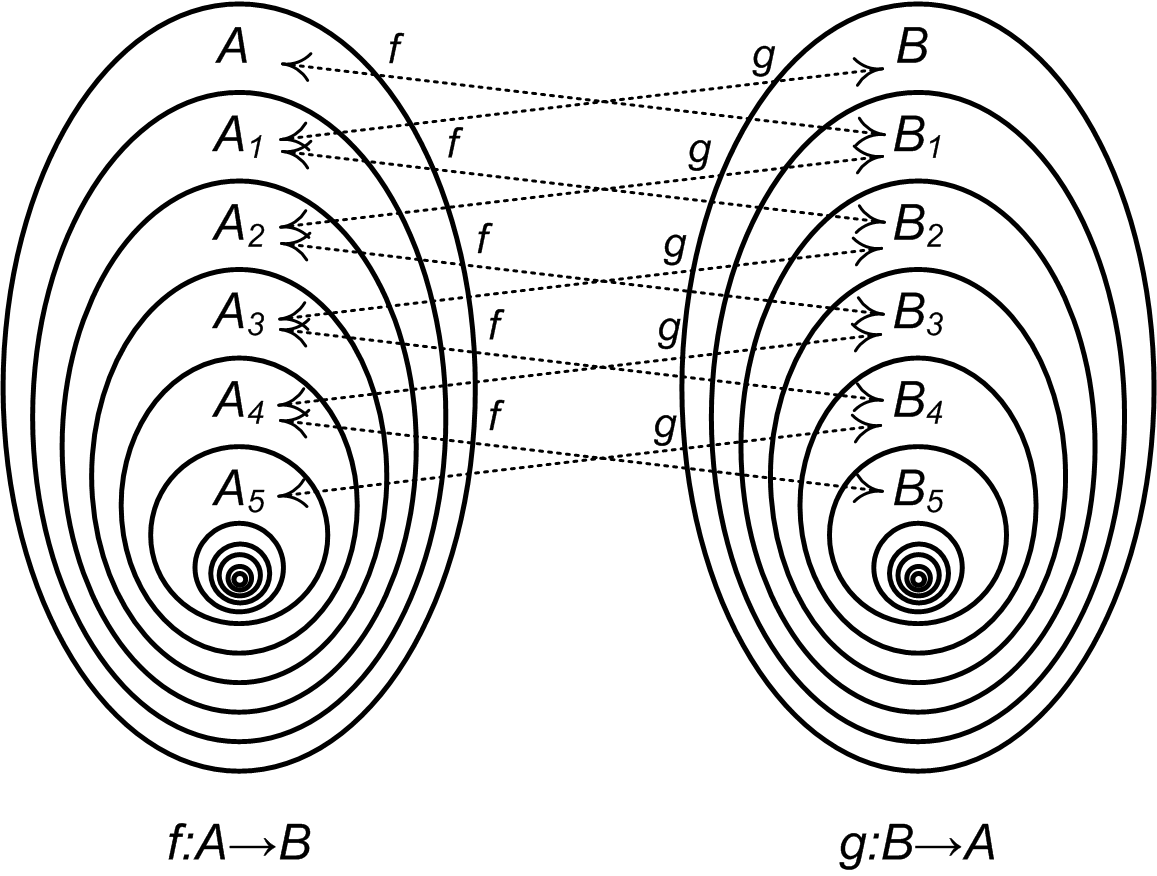
\includegraphics{fig/kantorBernstein1}
    \caption{$A\leq B$ и $B\leq A$}
    \label{fig:kantorBernstein1}
\end{figure} 

\begin{figure}
    \centering
    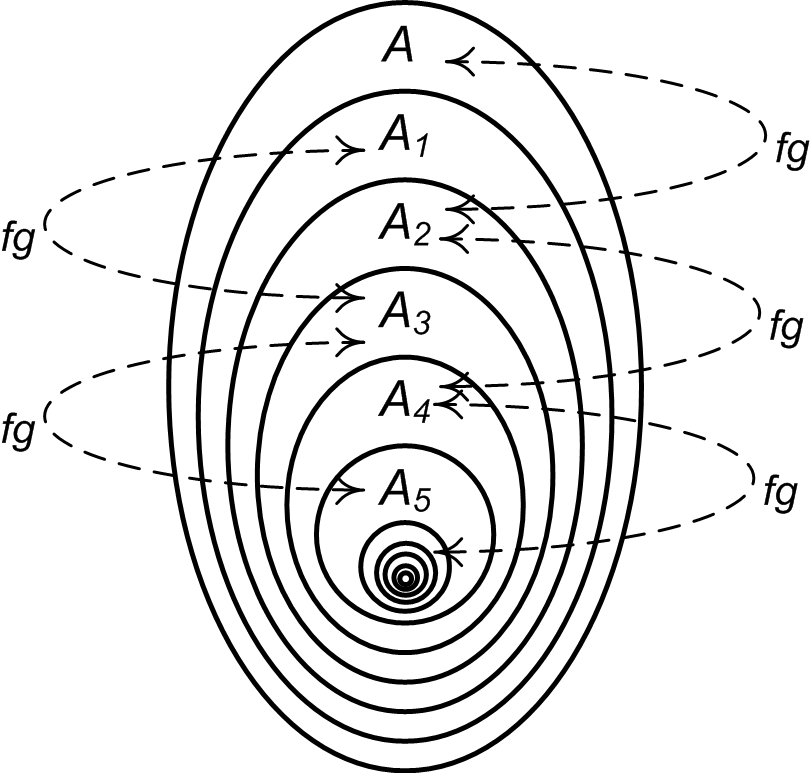
\includegraphics{fig/kantorBernstein2}
    \caption{$f\cdot g:M_{i}\leftrightarrow M_{i+2}$}
    \label{fig:kantorBernstein2}
\end{figure} 

\begin{figure}
    \centering
    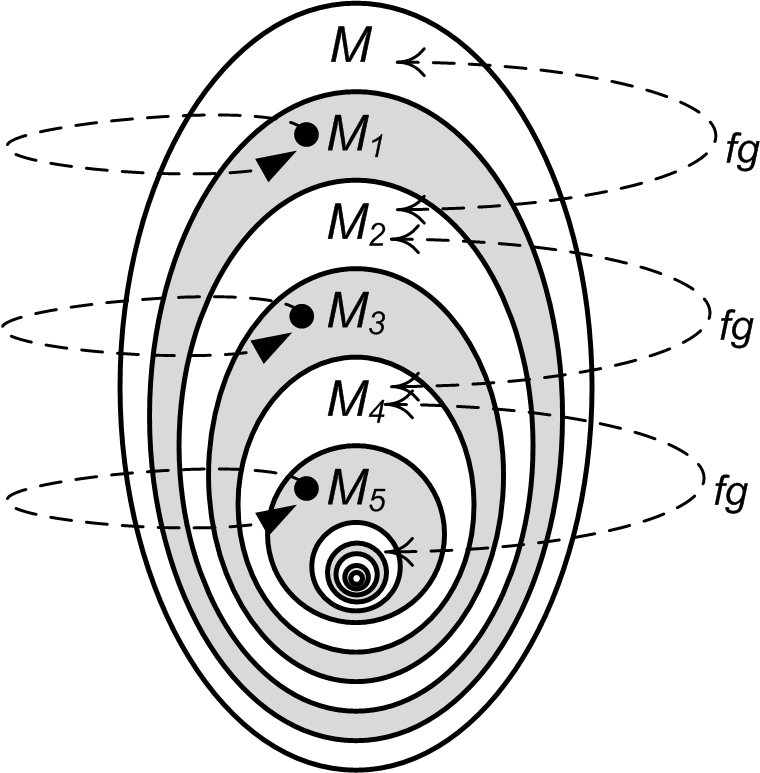
\includegraphics{fig/kantorBernstein3}
    \caption{Биекция $h:A\leftrightarrow A_1$}
    \label{fig:kantorBernstein3}
\end{figure} 

Из теоремы Кантора-Бернштейна следует, что для любых множеств $A$ и $B$ существует одна и только одна из трех возможностей:
\begin{enumerate}
    \item $|A|=|B|$;
    \item $|A|<|B|$;
    \item $|A|>|B|$.
\end{enumerate}

Мощность множества называют также \emph{кардинальным числом} или \emph{кардиналом}.  Кардинал характеризует целый \emph{класс} эквивалентных множеств. При решении практических задач часто требуется заменить некоторое множество на эквивалентное ему. При условии равенства кардиналов, это можно сделать.

Кардиналом для \emph{конечного} множества $A$ является натуральное число, равное количеству элементов множества $A$.

Для кардиналов \emph{конечных} множеств справедливо, например, что:
\begin{enumerate}
    \item Если $|A|=m$, $|B|=n$, то $|A\cup B|=m+n-|A\cap B|$;
    \item Если $|A|=m$, $|B|=n$, то $|A\times B|=m\cdot n$;
    \item Если $|A|=m$, $|B|=n$, то $|A^B|=m^n$.
\end{enumerate}

Видно, что кардиналы можно складывать, перемножать и возводить в степень.

Возведение множества в степень множества $A^B$ ранее не определялось. Множество $A^B$ состоит из всех возможных отображений множества $B$ на множество $A$:
\[
    A^B=\{f|f:B\to A\}.
\]

Например, булеан множества $M$, обозначается как $2^M$, где под <<$2$>> понимается любое двухэлементное множество, например, $\{0,1\}$. То есть <<$2$>> --- кардинал.
\begin{exampl} $M=\{a,b\}$. Булеан $2^M$ и множество $\{0,1\}^M$, эквивалентны:
    \[
    \begin{array}{c|c}
        2^M = \{          & \{0,1\}^M=\{                \\ \hline
        \{\emptyset\},    & \{a\mapsto 0, b\mapsto 0\}, \\
        \{a\},            & \{a\mapsto 1, b\mapsto 0\}, \\
        \{b\},            & \{a\mapsto 0, b\mapsto 1\}, \\
        \{a,b\}           & \{a\mapsto 1, b\mapsto 1\}  \\ \hline
        \}                &\}
    \end{array}
    \]
    \qed
\end{exampl}

Аналогично можно смотреть на степень множества $M^n$, где $n\in\mathbb{N}$ --- кардинал конечного множества.
\begin{exampl} $M=\{a,b\}$. $M^3$ и множество $M^{\{0,1,2\}}$, эквивалентны:
    \[
    \begin{array}{l||l}
        M^3 = \{    & M^{\{0,1,2\}}=\{              \\ \hline\hline
        \{a,a,a\},    & \{0\mapsto a, 1\mapsto a, 2\mapsto a\}, \\
        \{a,a,b\},    & \{0\mapsto a, 1\mapsto a, 2\mapsto b\}, \\
        \{a,b,a\},    & \{0\mapsto a, 1\mapsto b, 2\mapsto a\}, \\
        \{a,b,b\},    & \{0\mapsto a, 1\mapsto b, 2\mapsto b\}, \\
        \{b,a,a\},    & \{0\mapsto b, 1\mapsto a, 2\mapsto a\}, \\
        \{b,a,b\},    & \{0\mapsto b, 1\mapsto a, 2\mapsto b\}, \\
        \{b,b,a\},    & \{0\mapsto b, 1\mapsto b, 2\mapsto a\}, \\
        \{b,b,b\}     & \{0\mapsto b, 1\mapsto b, 2\mapsto b\}  \\ \hline\hline
        \}          &\}
    \end{array}
    \]
    \qed
\end{exampl}


\section{Мощность бесконечных множеств}

Для бесконечных множеств кардинал --- особое понятие. И при соответствующих операциях над бесконечными множествами такие кардиналы ведут себя по-особенному. 

Будь кардинал бесконечного множества обычным числом, то, например, можно было ожидать, что $|\mathbb{N}\times\mathbb{N}|=|\mathbb{N}^2|=\aleph_0^2$. Однако можно доказать, что $\mathbb{N}\times\mathbb{N}\sim\mathbb{N}$. То есть $|\mathbb{N}^2|=|\mathbb{N}|=\aleph_0$. 
\begin{exampl}
    $|\mathbb{N}^2|=|\mathbb{N}|=\aleph_0$.
\end{exampl}
\begin{proof}
    По определению множество $\mathbb{N}^2=\mathbb{N}\times\mathbb{N}$ задается как $\{(m,n)|m,n\in\mathbb{N}\}$. На координатной плоскости изобразим точки с натуральными координатами (см. рис. \ref{fig:diagonalKantor}). Если удастся построить биекцию $f:\mathbb{N}\leftrightarrow\mathbb{N}^2$, то тем самым докажем $|\mathbb{N}^2|=|\mathbb{N}|$. Видно:
    \[
        \begin{split}
            f:\mathbb{N}\leftrightarrow\mathbb{N}^2=\\
            \{
                0\mapsto(0,0),\\
                %
                1\mapsto(0,1),
                2\mapsto(1,0),\\
                %
                3\mapsto(0,2),
                4\mapsto(1,1),
                5\mapsto(2,0),\\
                %
                6\mapsto(0,3),
                7\mapsto(1,2),
                8\mapsto(2,1),
                9\mapsto(3,0),\\ \ldots
            \}
        \end{split}
    \]
\end{proof}

\begin{figure}
    \centering
    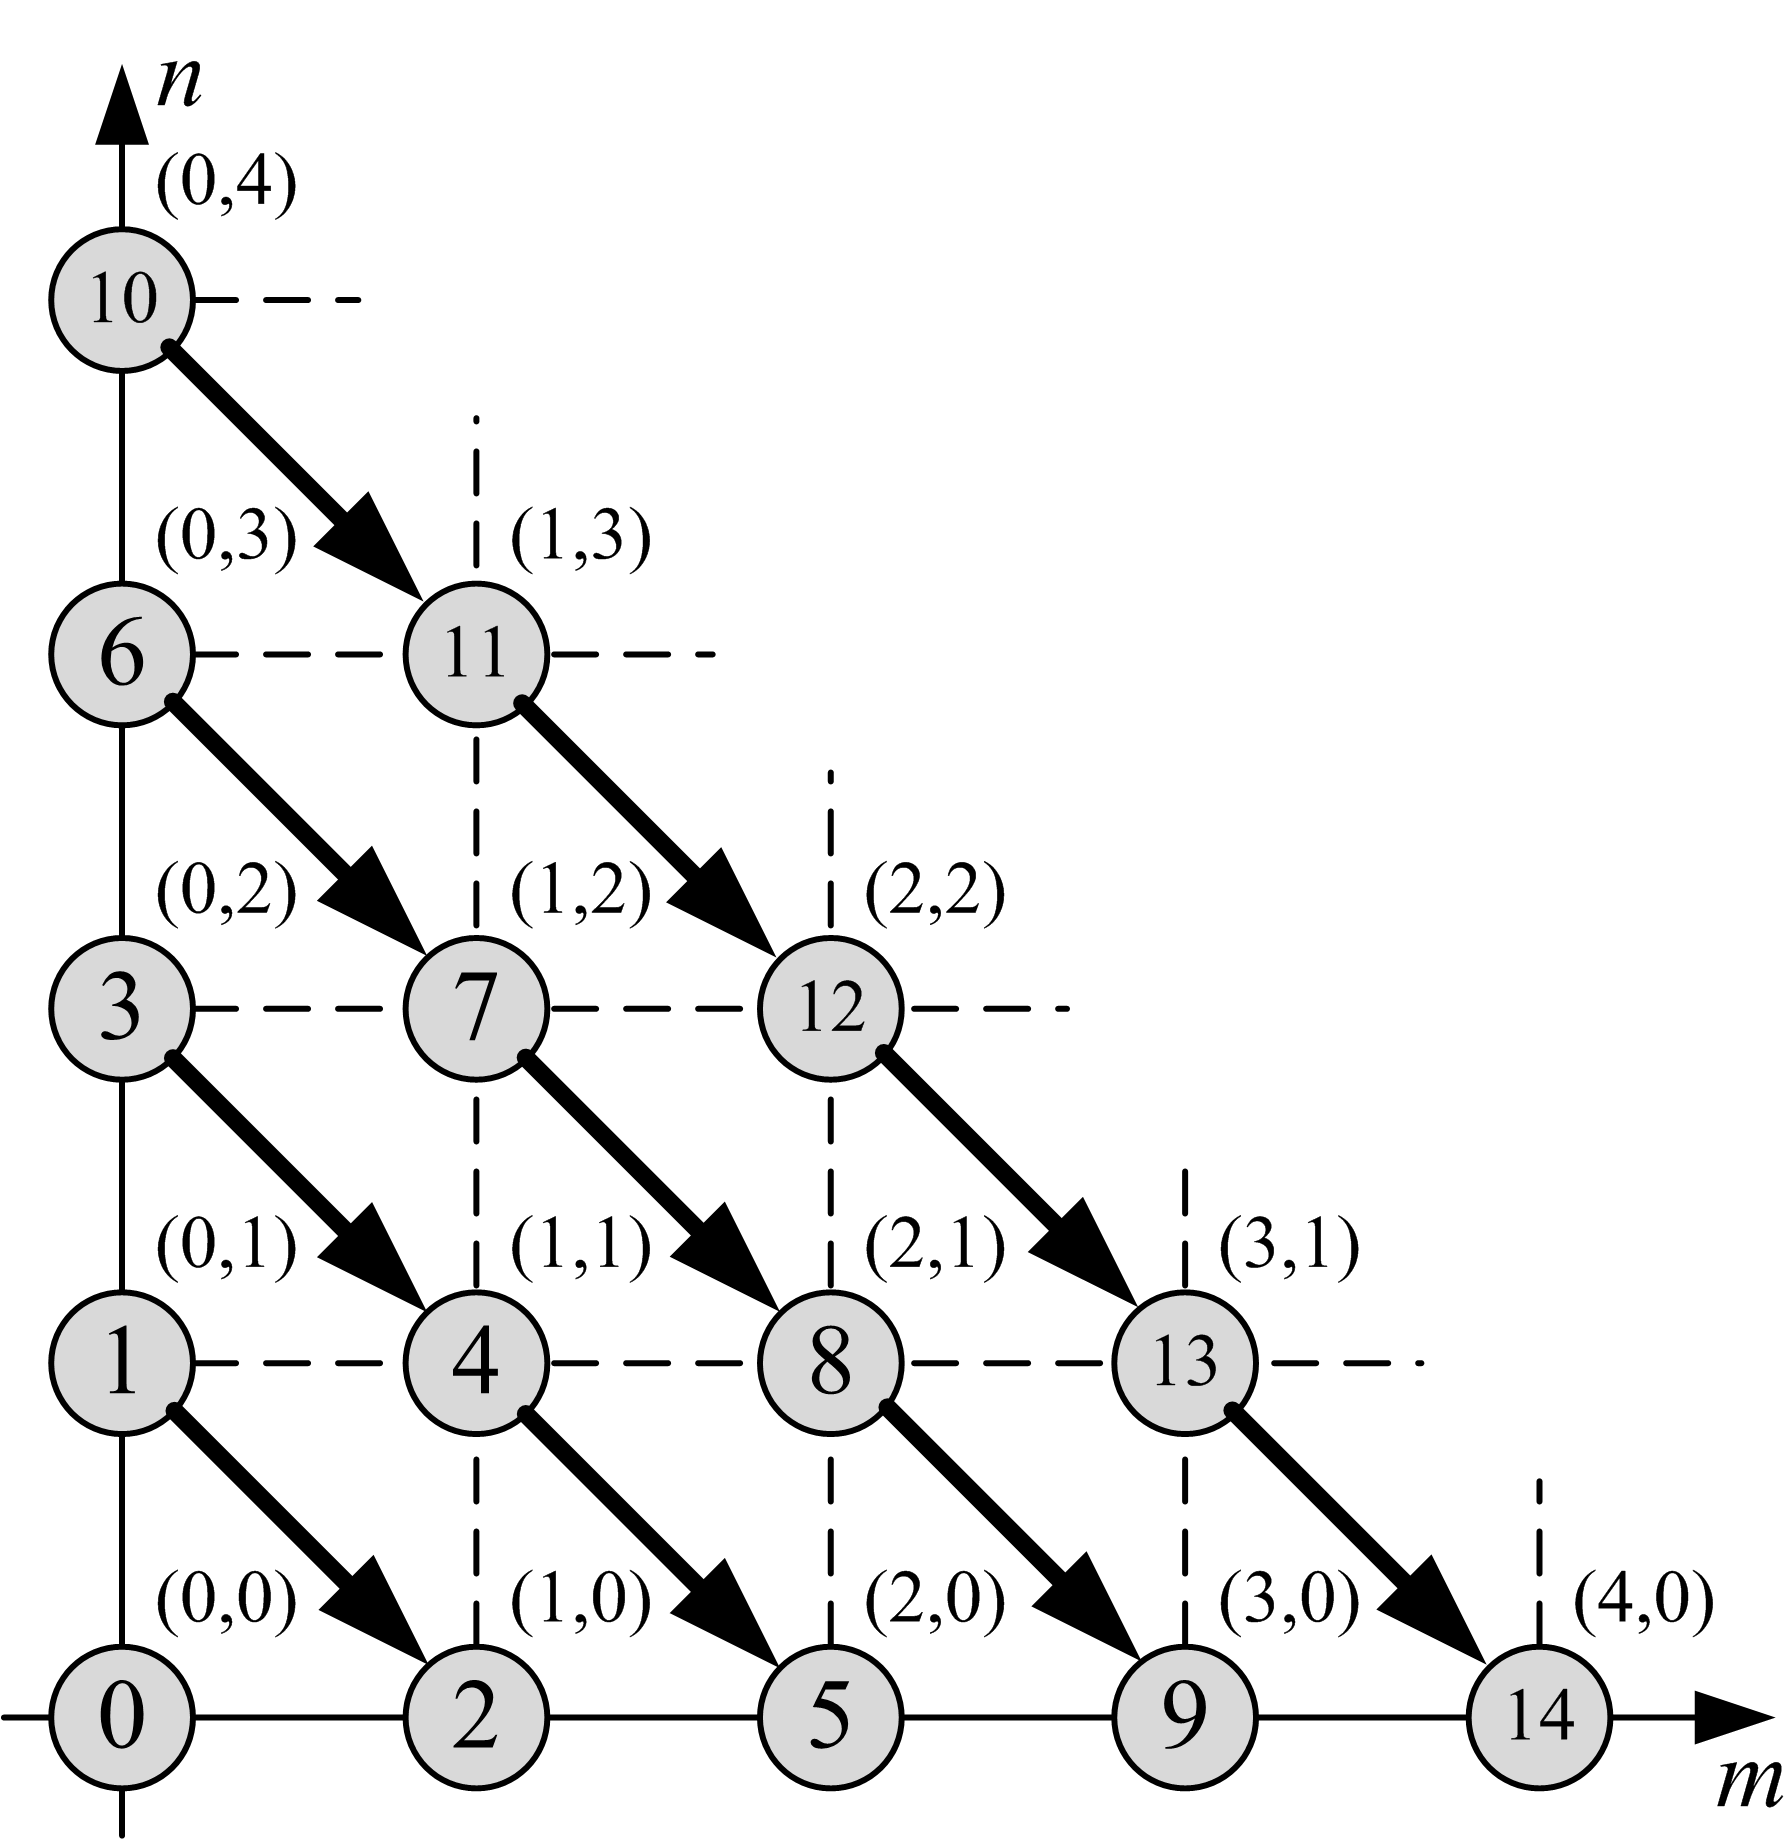
\includegraphics{fig/diagonalKantor}
    \caption{$f:\mathbb{N}\leftrightarrow\mathbb{N}^2$. Диагональная процедура Кантора}
    \label{fig:diagonalKantor}
\end{figure} 

Более того, справедливо, что:
\begin{itemize}
    \item $(\mathbb{N}\sim\mathbb{N}^n)\Leftrightarrow (|\mathbb{N}^n|=\aleph_0)$;
    \item $(\mathbb{N}\sim\bigcup_{n\in\mathbb{N}}\mathbb{N}^n) \Leftrightarrow (|\bigcup_{n\in\mathbb{N}}\mathbb{N}^n|=\aleph_0)$.
\end{itemize}

Но на $\aleph_0$ кардиналы бесконечных множеств не заканчиваются. Существуют бесконечные множества \emph{б\'{о}льших} мощностей.

\begin{Theor}[теорема Кантора]\label{ch:pwr:kantor}
    Для любого множества $M$ выполняется $|M|<2^{|M|}$.
\end{Theor}
\begin{proof}
    Так как для любого множества $M$ выполняется $|2^M|=2^{|M|}$, то необходимо показать, что $|M|\leq|2^M|$ и $|M|\neq|2^M|$. Функция $f:M\xrightarrow{\text{в}}2^M$, определенная по правилу $f(x)=\{x\}$, очевидно, инъективна, а тогда справедливо, что $|M|\leq|2^M|$. Теперь предположим, что $|M|=|2^M|$. Тогда существует биекция $\varphi:M\leftrightarrow 2^M$. Рассмотрим множество $K=\{x|x\in M,x\not\in\varphi(x)\}$. Поскольку $\varphi$ --- биекция и $K\subseteq M$, т.е. $K\in 2^M$, то существует $s\in M$, такое, что $\varphi(s)=K$. Если $s\in K$, то из определения $K$ получаем, что $s\not\in(K=\varphi(k))$. Если $s\not\in K$, то $s\not\in\varphi(s)$ и из определения $K$ следует, что должно выполняться $s\in K$. Противоречие показывает, что биекция $\varphi$ существовать не может.
\end{proof}

Для бесконечных множеств кардиналы имеют вид: $\aleph_0$, $2^{\aleph_0}$, $2^{2^{\aleph_0}}$,\ldots

\begin{exampl}
    $2^\mathbb{N}\sim 10^\mathbb{N}\sim \mathbb{N}^\mathbb{N}$.
\end{exampl}
\begin{proof}
    Поскольку неравенства $2^\mathbb{N}\leq 10^\mathbb{N}\leq \mathbb{N}^\mathbb{N}$ очевидны, то по теореме Кантора-Бернштейна (см. теорему \ref{Theor:KantorBernstain}) достаточно показать, что существует $\varphi:\mathbb{N}^\mathbb{N}\xrightarrow{\text{в}}2^\mathbb{N}$. Это фактически означает $\varphi$ кодирует все возможные последовательности натуральных чисел с помощью последовательностей из нулей и единиц. Для последовательности $f\in\mathbb{N}^\mathbb{N}$ 
    \[f=f_0f_1\cdots f_n\cdots\]
    определим последовательность $\varphi(f)\in 2^\mathbb{N}$ так:
    \[
        \underbrace{1,1,\ldots,1}_{f_0},0,
        \underbrace{1,1,\ldots,1}_{f_1},0,\ldots,0,
        \underbrace{1,1,\ldots,1}_{f_n},0,\ldots
    \]
    
    Определенная таким образом $\varphi$, очевидно является  биекцией. Например, если
    \[\varphi(f)=0,1,1,1,0,0,1,1,1,1,1,0\cdots\], то легко определяется \[f=0,3,0,5,\ldots\]
\end{proof}

Если $A\sim 2^{\mathbb{N}}$, то множество $A$ называется \emph{континуальным} или \emph{континуумом}: $|A|=2^{\aleph_0}$. Слово \emph{континуум} означает \emph{непрерывный}. Далее показано, например, что <<непрерывное>> множество вещественных чисел $\mathbb{R}$ эквивалентно всем возможным подмножествам множества натуральных чисел $2^\mathbb{N}$ и имеет мощность $|\mathbb{R}|=2^{\aleph_0}$.

\begin{exampl}
    $\mathbb{R}\sim [0,1]$
\end{exampl}
\begin{proof}
    Доказать, что мощности отрезка $[0,1]$ и интервала $(0,1)$ равны, можно задав биекцию:
    \[
        \varphi(x)=
        \begin{cases}
            x,&\text{если $x\neq 0,x\neq\frac{1}{n},n\in\mathbb{N},n>0)$},\\
            \frac{1}{2},&\text{если $x=0$},\\
            \frac{1}{3},&\text{если $x=1$},\\
            \frac{1}{n+2},&\text{если $x=\frac{1}{n},n\in\mathbb{N},n>1$}.\\
        \end{cases}
    \]
    В свою очередь биекция (см. рис. \ref{fig:tanIsContToR}) $\psi(x)=\tan(\pi(x-\frac{1}{2}))$ определяет эквивалентность интервала $(0,1)$ и множества $\mathbb{R}$. Тогда биекция $\psi(\varphi(x))$ определяет $[0,1]\sim\mathbb{R}$
\end{proof}

\begin{figure}
    \centering
    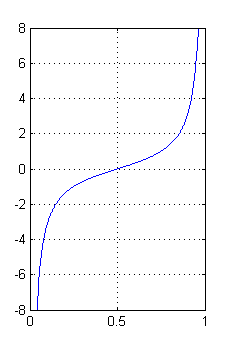
\includegraphics{fig/tanx}
    \caption{Биекция $\psi(x)=\tan(\pi(x-\frac{1}{2}))$}
    \label{fig:tanIsContToR}
\end{figure} 

Отрезок вещественной оси $[0,1]$ также называется континуумом.

\begin{Theor}
    $|\mathbb{R}|=2^{\aleph_0}$
\end{Theor}
\begin{proof}
    Любое вещественное число $X$ из $[0,1]$ можно задать в десятичном представлении бесконечной последовательностью:
    \[
        X\mapsto(0.a_1a_2\cdots a_n\cdots)_{10},
    \]
    где $n\in\mathbb{N}$ и $a_i\in\{0,\ldots,9\}$. При этом число определяется как
    \[
        X=\sum_{i\geq 1,i\in\mathbb{N}}a_i\cdot \frac{1}{10^i}.
    \]
    
    Видно, что $[0,1]\sim 10^\mathbb{N}$. Исходя из ранее доказанного:$10^\mathbb{N}\sim 2^\mathbb{N}$ и $\mathbb{R}\sim[0,1]$, заключаем $|\mathbb{R}|=2^{\aleph_0}$.
\end{proof}

Счетные и континуальные множества наиболее употребимы на практике. Но кардиналов бесконечных множеств (согласно теореме Кантора см. теорему \ref{ch:pwr:kantor}) бесконечно много, например $|2^\mathbb{R}|=2^{2^{\aleph_0}}$ --- множество всех подмножеств вещественных чисел мощнее континуума.


\section*{Задания}
\addcontentsline{toc}{section}{Задания}

\begin{enumerate}
    \item В группе из $40$ студентов все вычислители или отличники, и других нет. Вычислителей $30$, отличников $35$. Сколько вычислителей --- отличники?

    \item На острове $1000$ человек. Из них детей $400$, а взрослых женщин $350$. Сколько на острове 
    \begin{enumerate}
        \item женщин и детей?
        \item взрослых?
        \item взрослых мужчин?
    \end{enumerate}

    \item Сколько натуральных чисел в диапазоне $[1,200]$ делятся (+ не делятся) на:
    \begin{enumerate}
        \item $2$ или $3$;
        \item $6$ или $21$;
        \item $2$ или $3$ или $7$;
        \item $3$ или $10$ или $14$.
    \end{enumerate}
    
    \item Сколько натуральных чисел в диапазоне $[100,500]$ делятся (+ не делятся) на:
    \begin{enumerate}
        \item $3$ или $5$;
        \item $8$ или $12$;
        \item $4$ или $6$ или $15$;
        \item $6$ или $10$ или $15$.
    \end{enumerate}
    
    \item Доказать, что $|\mathbb{N}^3|=\aleph_0$.
    
    \item Каким числам соответствуют русские слова:
    \begin{enumerate}
        \item <<Я>>
        \item <<МАМА>>
        \item <<ПАПА>>
        \item <<ДОМ>>
        \item <<РОД>>
        \item <<ВЫСОКОПРЕВОСХОДИТЕЛЬСТВО>>\footnote{Дайте хотя бы оценку количества цифр в десятичном представлении этого числа}
    \end{enumerate}
    если 
    \[f:\text{Азбука}\to\mathbb{N} = 
        \text{
            \begin{tabular}{c|cccccccccc}
                f&0&1&2&3&4&5&6&7&8&9\\
                \hline
                 &А&Б&В&Г&Д&Е&Ё&Ж&З&И\\
                1&Й&К&Л&М&Н&О&П&Р&С&Т\\
                2&У&Ф&Х&Ц&Ч&Ш&Щ&Ъ&Ы&Ь\\
                3&Э&Ю&Я& & & & & & & 
            \end{tabular}
        }
    \]
    где <<$\text{Азбука}$>> --- русский алфавит.
    
    %множество всех слов конечного алфавита счетно $\aleph_0$
    %множество всех предложений из слов континуально ${\aleph_0}^{\aleph_0}$!
    %${\aleph_0}^{\aleph_0}=2^{\aleph_0}$.
    %$M\sim\mathbb{R}\sim[0,1]$
    \item Какова мощность множества $M$ всех возможных предложений из слов русского алфавита $T$?
    
    \item Множество всех пар из $\mathbb{N}^2$, оказывается счетно! Приведите функцию $f:\mathbb{N}^2\leftrightarrow\mathbb{N}$. Найдите $f(100,100)$. Найдите пару $(x,y)=f^{-1}(2048)$.

    
    \item Докажите, что множество рациональных чисел $\mathbb{Q}$ --- счетно.
    
    \item Приведите пример регулярного выражения, порождающего множество $M$, такое, что:
    \begin{enumerate}
        \item $|M|=7$;
        \item $|M|=\aleph_0$;
        \item $|M|=2^{\aleph_0}$.
    \end{enumerate}
    
    \item Приведите пример регулярных выражений, определяющих бесконечные регулярные множества $A$ и $B$, такие, что $A\subset B$ и $|A|=|B|$.
    
    \item Докажите, что диапазоны чисел $x\in\mathbb{R}$ эквивалентны:
    \begin{enumerate}
        \item $[0,1)\sim(0,1)$;
        \item $(0,1]\sim(0,1)$;
        \item $[0,1]\sim(0,1)$;
        \item $[m,n]\sim(0,1)$, $m,n\in\mathbb{N}$.        
    \end{enumerate}
    
\end{enumerate}
 %Мощность множества
    \chapter{Бинарные отношения на множестве $A$}
\label{ch:bo}
%bo: label prefix
Приводятся сведения о бинарных отношениях с особыми свойствами. Бинарные отношения активно применяются на практике. Специальные же бинарные отношения достойны особой роли, благодаря тем свойствам, которыми они обладают. Для углубленного изучения рекомендуются: \cite{bib:novic:discrmathprogrammer,bib:sudoplatov:discrmath,bib:shaporev:discretemath}.


\section{Свойства бинарных отношений на множестве $A$}

Напомним, что бинарным отношением $P$ на множестве $A$ называется $P\subseteq A^2$. 

Отношение $P$ на множестве $A$ называется.
\begin{enumerate}
    \item \emph{Рефлексивным ($\rho$)}, если для всех $x\in A$ справедливо $(x,x)\in P$.

    \item \emph{Антарефлексивным}, если для всех $x\in A$ справедливо $(x,x)\not\in P$.

    \item \emph{Симметричным ($\sigma$)}, если для любых $x,y\in A$ из $(x,y)\in P$ следует $(y,x)\in P$. То есть $P^{-1}=P$.

    \item \emph{Антисимметричным}, если для любых $x,y\in A$ из $(x,y)\in P\land(y,x)\in P$ следует $x=y$. То есть $P\cap P^{-1}\subseteq I_A$.    
    
    \item \emph{Транзитивным ($\eta$)}, если для любых $x,y\in A$ из $(x,y)\in P\land (y,z)\in P$ следует $(x,z)\in P$. То есть $P\cdot P\subseteq P$.
    
    \item \emph{Полным} или \emph{линейным}, если для любых $x,y\in A$ из $x\neq y$ следует $(x,y)\in P\lor (y,x)\in P$. То есть $U_A=I_A\cup P\cup P^{-1}$.
\end{enumerate}
 
Если бинарное отношение $P$ на множестве $A$ не обладает тем или иным свойством, то его можно дополнить упорядоченными парами из $A^2$ до отношения $P^*$, которое нужным свойством обладает. Если полученное $P^*$:
\begin{enumerate}
    \item обладает нужным свойством $S$ (обозначим $S(P^*)$);
    \item содержит $P$ ($P^*\supset P$);
    \item является подмножеством любого другого отношения $P'$, содержащего $P$ и обладающего свойством $S$ ($S(P')\land (P'\supset P)\Rightarrow P^*\subset P'$),
\end{enumerate}
то оно называется \emph{замыканием отношения $P$ относительно свойства $S$}.

Замыкания находят массу применений на практике. Особенную практическую ценность имеют замыкания относительно транзитивности. Например:
\begin{itemize}
    \item если задан граф коммуникационной сети, то найденное замыкание относительно транзитивности даст ответ на вопрос: существует ли возможность передать сообщение из одного узла в другой. 
    
    \item если на группе людей задано бинарное отношение <<родитель>>, то замыкание относительно транзитивности даст отношение <<предок>>.
\end{itemize}
    
\begin{exampl}
    На множестве $\{1,2,3\}$ задано бинарное отношение 
    \[P=\{(1,1),(1,2),(1,3),(3,1),(2,3)\},\]
    которое не обладает свойствами рефлексивности, симметричности и транзитивности. Необходимо найти соответствующие замыкания.
    
    До обладания свойством рефлексивности нужно добавить 2 пары: \[\{(2,2),(3,3)\}.\]
    
    До обладания свойством симметричности нужно добавить также 2 пары: \[\{(2,1),(3,2)\}.\]
    
    Процесс поиска замыкания относительно транзивности состоит из нескольких шагов.
    \begin{enumerate}
        \item Для пар $(3,1)$ и $(1,2)$ нужна пара $(3,2)$.
        \item Для пар $(2,3)$ и $(3,1)$ нужна пара $(2,1)$.\label{enumer:transClosureEx1}
        \item Для пар $(3,1)$ и $(1,3)$ нужна пара $(3,3)$.
        \item Для пар $(2,1)$ и $(1,2)$ нужна пара $(2,2)$. Внимание:пара $(2,1)$ добавилась на шаге \ref{enumer:transClosureEx1}.
    \end{enumerate}
    \qed
\end{exampl}

Близость $\Delta(P,S)$ бинарного отношения $P$ к некоторому свойству $S$ можно оценивать количеством \emph{добавленных} или \emph{удаленных} пар (см. рис. \ref{fig:nearnessOfBinRelations}).

\begin{figure}
    \centering
    \begin{tabular}{cccc}
        {\xymatrix{
            a \ar@{->}[d] \ar@{->}[r]
                &d \ar@{->}[d]
                    \\
            b \ar@{->}[r]
                &c
        }}
            &
            {\xymatrix{
                a \ar@{->}[d] \ar@{->}[r] \ar@{.>}@(l,u)[]
                    &d \ar@{->}[d] \ar@{.>}@(u,r)[]
                        \\
                b \ar@{->}[r] \ar@{.>}@(d,l)[]
                    &c \ar@{.>}@(r,d)[]
            }}
                &
                {\xymatrix{
                    a \ar@{->}[d] \ar@{->}[r]
                        &d \ar@{->}[d] \ar@{.>}@/_/[l] 
                            \\
                    b \ar@{->}[r] \ar@{.>}@/^/[u] 
                        &c \ar@{.>}@/^/[l] \ar@{.>}@/_/[u] 
                }}
                    &
                    {\xymatrix{
                        a \ar@{->}[d] \ar@{->}[r] \ar@{.>}[dr]
                            &d \ar@{->}[d]
                                \\
                        b \ar@{->}[r]
                            &c
                    }}
                \\
                &&&\\
            Исходное $P$ 
                & Рефлексивное($\rho$) 
                    & Симметричное($\sigma$) 
                        & Транзитивное($\eta$)\\
                & $\Delta(P,\rho)=4$ 
                    & $\Delta(P,\sigma)=4$ 
                        & $\Delta(P,\eta)=1$ 
    \end{tabular}
    \caption{Близость бинарных отношений к свойствам}
    \label{fig:nearnessOfBinRelations}
\end{figure}

Поиск транзитивных замыканий отношений представляет наибольшую сложность. Человек может найти транзитивное замыкание, глядя на орграф отношения, что неприемлемо для машины. Приведенный псевдокод для алгоритма Уоршалла (см. псевдокод \ref{alg:bo:warshall}) позволяет найти транзитивное замыкание отношения, представленного матрицей смежности. 

Обоснование данного алгоритма на соответствующем отношению $P$ графе следующее. Первой итерацией внешнего цикла ($k=1$) к исходному графу будут добавлены транзитивные дуги, замыкающие путь через $a_1$ ($P\subseteq A^2, a_i\in A$). $k$-й итерацией будут добавлены транзитивные дуги, замыкающие путь через <<пройденные транзитом>> вершины $a_1,\ldots,a_k$. Последней итерацией $k=n$ будут добавлены дуги, проходящие транзитом через \emph{любую} последовательность из $n$ вершин графа.

\begin{algorithm}
    \caption{Поиск транзитивного замыкания $P$ (алгоритм Уоршалла)}\label{alg:bo:warshall}
    \begin{algorithmic}[1]
        \REQUIRE{$[P]_{n\times n}$ --- матрица смежности отношения $P$}
        \ENSURE{$[T]_{n\times n}$ --- матрица транзитивного замыкания отношения $P$}
        \STATE{$[T]\gets [P]$}
        \FOR{$k=1$ to $n$}
            \FOR{$i=1$ to $n$}
                \FOR{$j=1$ to $n$}
                    \STATE{$[T]_{i,j}\gets\big([T]_{i,j}\lor ([T]_{i,k}\land[T]_{k,j})\big)$}
                \ENDFOR
            \ENDFOR
        \ENDFOR
    \end{algorithmic}
\end{algorithm}
    
    
\section{Специальные бинарные отношения на множестве $A$}

Некоторые бинарные отношения имеют большое практическое значение. Следует изучить их подробнее.


\subsection{Отношение эквивалентности}
 

Бинарное отношение на множестве $A$, обладающее свойствами рефлексивности ($\rho$), симметричности ($\sigma$) и транзитивности ($\eta$), называется отношением \emph{эквивалентности}\footnote{Это отношение уже упоминалось при обсуждении темы мощности множеств} и обозначается $\sim$ или $\equiv$. Эквивалентность является  обобщением равенства\footnote{Равенство обладает ярко выраженной рефлексивностью --- это тождественное отношение $I_A$. $(x,x)\in =$. Но видно, что и в симметричности с транзитивностью ему не откажешь\ldots Равенство --- частный случай эквивалентности}.

\emph{Классом эквивалентности} $E(x)$ элемента $x\in A$ называется множество всех элементов $y\in A$, каждый из которых находится в отношении эквивалентности $E$ с элементом $x$:
\[E(x)=\{y|x\,E\,y, x\in A, y\in A\}\]

Множество, обозначаемое $A/E$:
\[
    A/E=\{E(x)|x\in A\},
\]
называется \emph{фактор-множеством} множества $A$ по отношению эквивалентности $E$.

\begin{Theor}
    Всякое отношение эквивалентности $E$ на множестве $A$ определяет \emph{разбиение}, которым явлеется \emph{фактор-множество} $A/E$. И обратно: всякое разбиение 
    \[
        \mathcal{R}=\{A_i|i\in \mathbb{N}, A_i,\subseteq A,(i\neq j)\Rightarrow (A_i\cap A_j=\emptyset)\},A=\bigcup_{i\in\mathbb{N}} A_i
    \]
    множества $A$, не содержащее пустых элементов, определяет отношение эквивалентности $E$ на $A$ по правилу \begin{equation}
        x\,E\,y\Leftrightarrow x,y\in A_i.
        \label{eq:bo:equivByR}
    \end{equation}
\end{Theor}
\begin{proof}
    Так как $E$ рефлексивно, то $x\in E(x)$ для любого $x\in A$. Отсюда следует, что каждое множество из $A/E$ непусто и $\bigcup_{x\in A}E(x)=A$. Чтобы доказать, что $A/E$ является разбиением достаточно доказать, что если $E(x)\cap E(y)\neq\emptyset$, то $E(x)=E(y)$.
    
    Покажем, что $E(x)\subseteq E(y)$ и $E(y)\subseteq E(x)$ при $E(x)\cap E(y)\neq\emptyset$. Пусть $z\in E(x)\cap E(y)$. Докажем $E(x)\subseteq E(y)$. Возьмем $k\in E(x)$, тогда справедливо $k\,E\,z$, $z\,E\,y$ и, следовательно, $k\,E\,y$. Если $k\,E\,y$, то $k\in E(y)$. Стало быть $k\in E(x)\Rightarrow k\in E(y)$, а значит $E(x)\subseteq E(y)$. Аналогично докажем, что $E(y)\subseteq E(x)$.\qed
    
    Теперь докажем обратное утверждение теоремы. Пусть имеется разбиение $\mathcal{R}=\{A_i\}$. Рефлексивность и симметричность $E$, определяемого формулой \eqref{eq:bo:equivByR} очевидны. Докажем транзитивность. $x\,E\,y$ справедливо при $x,y\in A_i$, $y\,E\,z$ --- при $y,z\in A_j$. Но раз $y\in A_i$ и $y\in A_j$, то $A_i=A_j$. Тогда справедливо $x,z\in A_i$ и $x\,E\,z$.
\end{proof}

В любом классе $E(x)$ эквивалентности $E$ каждый элемент $y\in E(x)$ связан отношением $E$ с любым $z\in E(x)$. Поэтому, если 
\[
    A/E=\{\{a^1_1,\ldots,a^1_{m_1}\},\{a^2_1,\ldots,a^2_{m_2}\},\ldots,\{a^n_1,\ldots,a^n_{m_n}\}\}
\]
и элементы множества $A$ упорядочены так:
\[
    a^1_1,\ldots,a^1_{m_1},a^2_1,\ldots,a^2_{m_2},\ldots,a^n_1,\ldots,a^n_{m_n},
\]
то матрица смежности отношения $E$ имеет блочно - диагональный вид:
\[[E]=
    \begin{array}{c|cccc}
        E
            &a^1_1\cdots a^1_{m_1} 
                & a^2_1\cdots a^2_{m_2} 
                    & \cdots 
                        & a^n_1\cdots a^n_{m_n}
                            \\ 
        \hline
        \begin{matrix}a^1_1\\ \vdots \\ a^1_{m_1}\end{matrix} 
            &\begin{array}{|ccc|}\hline 1&\cdots&1\\ \vdots & \ddots & \\ 1 & & 1\\ \hline\end{array}
                &
                    &
                        &
                            \\
        \begin{matrix}a^2_1\\ \vdots \\ a^2_{m_2}\end{matrix} 
            &
                &\begin{array}{|ccc|}\hline 1&\cdots&1\\ \vdots & \ddots & \\ 1 & & 1\\ \hline\end{array}
                    &
                        & 
                            \\
        \vdots
            &
                &
                    &\ddots
                        & 
                            \\
        \begin{matrix}a^n_1\\ \vdots \\ a^n_{m_n}\end{matrix} 
            &
                &
                    &
                        &\begin{array}{|ccc|}\hline 1&\cdots&1\\ \vdots & \ddots & \\ 1 & & 1\\ \hline\end{array}
    \end{array},
\]
где квадратные непересекающиеся блоки на главной диагонали состоят из единиц, а остальные элементы равны нулю.

Если множество $A$ таким образом не упорядочено, то соответствующая матрица смежности $[E]$ приводится к блочно-диагональному виду одновременными перестановками строк и столбцов. Элементы $a_i$ и $a_j$ эквивалентны тогда и только тогда, когда $i$-я и $j$-я строки (а также столбцы) матрицы $[E]$ совпадают. Класс эквивалентности $E(a_i)$ состоит из элементов $a_j$, для которых $[E]_{ij}=1$.

\begin{exampl}
    Задача. Пусть имеется, например, численный рассчет, представленный орграфом на рисунке \ref{fig:bo:calcFlowEx}. Исходным данным соответствует $S$, конечному результату --- $R$. Вершинам графа соответствуют операции $O_i$. Дуге, соединяющей операции $O_i$ и $O_j$ соответствует численный результат $r_i$ полученный на выходе операции $O_i$ и подаваемый на вход операции $O_j$. Так как исходные данные (или их часть) для операции $O_j$ вычисляются операцией $O_i$, то $O_j$ всегда выполняется во времени \emph{позже} $O_i$. Операции, представленные на графе на одной вертикали, в общем случае могут быть выполнены параллельно. Необходимо минимизировать затраты памяти для хранения промежуточных результатов $r_i$, предполагая, что все они занимают одинаковый объем.
\end{exampl}

\begin{figure}
    \centering
    \[
    {\xymatrix{
        *{}
            &O_1\ar@{->}[rr]^{r_1}
                &*{}
                    &O_5 \ar@{->}[r]^{r_5}
                        &O_7 \ar@{->}[dr]^{r_7}
                            &*{}
                                &*{}
                \\
        *{S} \ar@{-->}[ur] \ar@{-->}[dr] \ar@{-->}[rr]
            &*{}
                &O_3 \ar@{->}[r]^{r_3} \ar@{->}[ur]^{r_3}
                    &O_6 \ar@{->}[rr]^{r_6}
                        &*{}
                            &O_8 \ar@{=>}[r]
                                &*{R}
                \\
        *{}
            &O_2 \ar@{->}[r]^{r_2} \ar@{->}[ur]^{r_2}
                &O_4 \ar@{->}[ur]^{r_4} \ar@{->}[urrr]^{r_4}
                    &*{}
                        &*{}
                            &*{}
                                &*{}
                \\
    }}
    \]
    \caption{Граф потока вычислений}
    \label{fig:bo:calcFlowEx}
\end{figure}

\begin{proof}[Решение]
    Решая задачу \emph{грубой силой и невежеством}\footnote{Сокращенно: ГСН-алгоритм.}, можно для хранения каждого промежуточного результата $r_i$ использовать отдельную ячейку $m_i$. Кроме того, для сохранения исходных данных и окончательного результата нужно еще две ячейки: $m_S$, $m_R$. См. не оптимизированный по памяти вариант программы в таблице \ref{table:bo:calcFlowProgramEx}. Итого 9 ячеек.
    
    Результат можно сделать лучше, заметив, что времена жизни некоторых результатов не пересекаются во времени! Это значит, что для них можно использовать одну ячейку. Например, использовать для хранения $r_1$ и $r_2$ одну ячейку нельзя, а вот $r_1$ и $r_5$ можно: $r_1$ после вычисления $r_5$ уже не нужен. Введем отношение $\not\perp$, означающее: <<времена жизни не пересекаются>>. Это отношение, очевидно:
    \begin{itemize}
        \item симметрично $(r_i\not\perp r_j)\Rightarrow (r_j\not\perp r_i)$; 
        \item рефлексивно $r_i\not\perp r_i$.
    \end{itemize}
    Увы, оно не транзитивно: например, $r_1\not\perp r_5$ и $r_5\not\perp r_3$, но $r_1$ и $r_3$ в отношении $\not\perp$ не находятся. Тем не менее, так как указанное отношение рефлексивно, то оно содержит по крайней мере тождественное отношение (которое есть отношение эквивалентности), а может быть и какое-то другое отношение эквивалентности.
    
    Построим матрицу смежности для отношения $\not\perp$:
    \[
        \begin{array}{c|ccccccccc}
            \not\perp
                & S &r_1&r_2&r_3&r_4&r_5&r_6&r_7& R\\ \hline
            S   & 1 & 0 & 0 & 1 & 1 & 1 & 1 & 1 & 1\\
            r_1 & 0 & 1 & 0 & 0 & 0 & 1 & 1 & 1 & 1\\
            r_2 & 0 & 0 & 1 & 1 & 1 & 1 & 1 & 1 & 1\\
            r_3 & 1 & 0 & 1 & 1 & 0 & 1 & 1 & 1 & 1\\
            r_4 & 1 & 0 & 1 & 0 & 1 & 0 & 0 & 0 & 1\\
            r_5 & 1 & 1 & 1 & 1 & 0 & 1 & 0 & 1 & 1\\
            r_6 & 1 & 1 & 1 & 1 & 0 & 0 & 1 & 0 & 1\\
            r_7 & 1 & 1 & 1 & 1 & 0 & 1 & 0 & 1 & 1\\
            R   & 1 & 1 & 1 & 1 & 1 & 1 & 1 & 1 & 1
        \end{array}
    \]
    
    Перестановкой строк и столбцов можно получить такую матрицу смежности:
    \[
        \begin{array}{c|ccccccccc}
            \not\perp
                & R &r_1&r_5&r_7&r_3&r_6& S &r_2&r_4\\\hline
            R   & 1 & 1 & 1 & 1 & 1 & 1 & 1 & 1 & 1\\
            r_1 & 1 & 1 & 1 & 1 & 0 & 1 & 0 & 0 & 0\\
            r_5 & 1 & 1 & 1 & 1 & 1 & 0 & 1 & 1 & 0\\
            r_7 & 1 & 1 & 1 & 1 & 1 & 0 & 1 & 1 & 0\\
            r_3 & 1 & 0 & 1 & 1 & 1 & 1 & 1 & 1 & 0\\
            r_6 & 1 & 1 & 0 & 0 & 1 & 1 & 1 & 1 & 0\\
            S   & 1 & 0 & 1 & 1 & 1 & 1 & 1 & 0 & 1\\
            r_2 & 1 & 0 & 1 & 1 & 1 & 1 & 0 & 1 & 1\\
            r_4 & 1 & 0 & 0 & 0 & 0 & 0 & 1 & 1 & 1
        \end{array}
    \]
    
    Видно, что легко выделяется (удалением пар) содержащееся в нем отношение эквивалентности с тремя классами $\{R,r_1,r_5,r_7\}$, $\{S,r_3,r_6\}$ и $\{r_2,r_4\}$:
    \[
        \begin{array}{c|ccccccccc}
            \not\perp
                & R &r_1&r_5&r_7&r_3&r_6& S &r_2&r_4\\\hline
            R   & 1 & 1 & 1 & 1 & 0 & 0 & 0 & 0 & 0\\
            r_1 & 1 & 1 & 1 & 1 & 0 & 0 & 0 & 0 & 0\\
            r_5 & 1 & 1 & 1 & 1 & 0 & 0 & 0 & 0 & 0\\
            r_7 & 1 & 1 & 1 & 1 & 0 & 0 & 0 & 0 & 0\\
            r_3 & 0 & 0 & 0 & 0 & 1 & 1 & 1 & 0 & 0\\
            r_6 & 0 & 0 & 0 & 0 & 1 & 1 & 1 & 0 & 0\\
            S   & 0 & 0 & 0 & 0 & 1 & 1 & 1 & 0 & 0\\
            r_2 & 0 & 0 & 0 & 0 & 0 & 0 & 0 & 1 & 1\\
            r_4 & 0 & 0 & 0 & 0 & 0 & 0 & 0 & 1 & 1
        \end{array}
    \]
    
    Данные результатов одного класса эквивалентности можно хранить в одной ячейке. Оказывается, можно использовать три ячейки: в $m_1$ хранить данные класса $\{R,r_1,r_5,r_7\}$, в $m_2$ --- $\{S,r_3,r_6\}$ и в $m_3$ --- $\{r_2,r_4\}$. Пример программы до и после оптимизации представлен в таблице \ref{table:bo:calcFlowProgramEx}. Полученные две программы, очевидно, имеют отличия, но они дают одинаковые результаты. Такие программы называют \emph{эквивалентными}. Конечно, эквивалентные программы могут отличаться не только затратами памяти, но и, например, скоростью получения результата.
    
    \begin{table}
        \centering
        \begin{tabular}{l||l}
            \hline\hline
            До оптимизации --- 9 я.п.      & После оптимизации --- 3 я.п.   \\
            \hline\hline
            $S \to m_S$                    &  $S\to m_2$                    \\ \hline
            $O_1(m_S)\to r_1 \to m_1$      &  $O_1(m_2)\to r_1 \to m_1$     \\
            $O_2(m_S)\to r_2 \to m_2$      &  $O_2(m_2)\to r_2 \to m_3$     \\ \hline
            $O_3(m_S,m_2)\to r_3 \to m_3$  &  $O_3(m_2,m_3)\to r_3 \to m_2$ \\
            $O_4(m_2)\to r_4 \to m_4$      &  $O_4(m_3)\to r_4 \to m_3$     \\ \hline
            $O_5(m_1,m_3)\to r_5 \to m_5$  &  $O_5(m_1,m_2)\to r_5 \to m_1$ \\
            $O_6(m_3,m_4)\to r_6 \to m_6$  &  $O_6(m_2,m_3)\to r_6 \to m_2$ \\ \hline
            $O_7(m_5)\to r_7 \to m_7$      &  $O_7(m_1)\to r_7 \to m_1$     \\ \hline
            $O_8(m_4,m_6,m_7)\to R \to m_R$&  $O_8(m_3,m_2,m_1)\to R\to m_1$\\ \hline
        \end{tabular}
        \caption{Эквивалентные программы с разными затратами памяти}
        \label{table:bo:calcFlowProgramEx}
    \end{table}    
\end{proof}


\subsection{Отношение порядка}

Отношение \emph{порядка} является обобщением отношения $\leq$, например, на натуральных числах. Выделяют несколько видов отношений порядка. В общем случае отношение порядка обозначается $\prec$, когда неважно, о каком его виде идет речь. Свойства всех отношений порядка таковы, что обратное отношение также является отношением порядка. Обратное отношение $\prec^{-1}$ обозначается $\succ$. Если на множестве $A$ задано некоторое отношение порядка $\prec$, то это обозначается $\langle A,\prec\rangle$.

\begin{enumerate}
    \item Отношение \emph{частичного} порядка рефлексивно, транзитивно и антисимметрично. Обозначается символом $\leq$, обратное отношение $\geq$. Множество $A$ над элементами которого задано отношение частичного порядка, называется \emph{частично упорядоченным множеством}. Пример частичного порядка --- отношение $\subseteq$ на булеане множества $M$ (см. рис. \ref{fig:bo:ordersEx})
    
    \item Отношение \emph{строгого} порядка транзитивно, антисимметрично и антирефлексивно. Обозначается символом $<$, а обратное символом $>$. То есть
    \[(x<y)\Leftrightarrow (x\leq y)\land(x\neq y).\]
    Примером строгого порядка явлеется отношение $<$ на $\mathbb{N}$ (см. рис. \ref{fig:bo:ordersEx}).
    
    \item Отношение \emph{линейного} порядка, представляет собой отношение частичного порядка, в котором отсутствуют несравнимые элементы. То есть для любых $x,y$ справедливо, что $x\leq y$ или $y\leq x$. То есть отношение рефлексивно, транзитивно, антисимметрично и полно. Множество $A$, над элементами которого задано отношение линейного порядка, называется \emph{линейно упорядоченным множеством}. Примером линейного порядка явлеется отношение $\leq$ на $\mathbb{N}$ (см. рис. \ref{fig:bo:ordersEx}).
\end{enumerate}

\begin{figure}
    \centering
    \begin{tabular}{ccc}
        {\xymatrix{
            *{}
                &\{1,2\} \ar@{->}@(ul,ur)[]
                    &*{}
                        \\
            \{1\}  \ar@{->}@(dl,ul)[] \ar@{->}[ur]
                &*{} 
                    &\{2\} \ar@{->}@(ur,dr)[] \ar@{->}[ul]
                        \\
            *{} 
                &\emptyset \ar@{->}@(dr,dl)[] \ar@{->}[ul] \ar@{->}[ur] \ar@{->}[uu]
                    &*{} 
        }}
            &
            {\xymatrix{
                *{}
                    &4 
                        &*{}
                            \\
                2  \ar@{->}[ur] \ar@{->}[rr] 
                    &*{} 
                        &3 \ar@{->}[ul]
                            \\
                *{} 
                    &1 \ar@{->}[ul] \ar@{->}[ur] \ar@{->}[uu]
                        &*{} 
            }}
                &
                {\xymatrix{
                    *{}
                        &4 \ar@{->}@(ul,ur)[]
                            &*{}
                                \\
                    2  \ar@{->}@(dl,ul)[] \ar@{->}[ur] \ar@{->}[rr] 
                        &*{} 
                            &3 \ar@{->}@(ur,dr)[] \ar@{->}[ul]
                                \\
                    *{} 
                        &1 \ar@{->}@(dr,dl)[] \ar@{->}[ul] \ar@{->}[ur] \ar@{->}[uu]
                            &*{} 
                }}
                    \\
        &&\\
        $\subseteq$ на $2^{\{1,2\}}$
            &$<$ на $\{1,2,3,4\}$
                & $\leq$ на $\{1,2,3,4\}$
                    \\
        Частичный порядок
            &Строгий порядок
                &Линейный порядок
    \end{tabular}
    \caption{Отношения порядка}
    \label{fig:bo:ordersEx}
\end{figure}    
    
Элемент $a\in A$ частично упорядоченного множества $A$ называется \emph{минимальным}, если для всех $x\in A$ из $x\leq a$ следует $a=x$. Элемент $a\in A$ частично упорядоченного множества $A$ называется \emph{максимальным}, если для всех $x\in A$ из $a\leq x$ следует $a=x$. Минимальных (максимальных) элементов в частично упорядоченном множестве может быть несколько и их не может не быть.

Элемент $a\in A$ частично упорядоченного множества $A$ называется \emph{наименьшим}, если для всех $x\in A$ справедливо $a\leq x$. Элемент $a\in A$ частично упорядоченного множества $A$ называется \emph{наибольшим}, если для всех $x\in A$ справедливо $x\leq a$. 
\begin{Theor}
    Частично упорядоченное множество содержит не более одного наименьшего (наибольшего) элемента.
\end{Theor}
\begin{proof}    
    Допустим, что в множестве более одного наименьшего элемента. Допустим, что $a_1$, $a_2$ --- два из этих элементов, тогда справедливо, что $a_1\leq a_2$ и $a_2\leq a_1$, стало быть $a_1=a_2$. Аналогичго можно доказать теорему для наибольшего элемента.
\end{proof}

В качестве следствия этой теоремы можно отметить, что наименьшего (наибольшего) элемента может и не быть, а также то, что наименьший (наибольший) элемент также будет минимальным (максимальным). См., например, рисунок \ref{fig:bo:minMaxEx}: наибольший (он же максимальный) элемент --- $c$, минимальные элементы --- $a,b$, наименьшего элемента нет.

Наименьший элемент частично упрядоченного множества $A$ обозначается $\min{A}$, а наибольший $\max{A}$.
\begin{figure}
    \centering
    \[
    {\xymatrix{
        a \ar@{->}@(dl,ul)[] \ar@{->}[r]
            &c \ar@{->}@(ur,dr)[]
                \\
        b  \ar@{->}@(dl,ul)[] \ar@{->}[ur]
            &*{}                 
    }}
    \]
    \caption{Частично упорядоченное множество $\langle\{a,b,c\},\leq\rangle$}
    \label{fig:bo:minMaxEx}
\end{figure}    

\emph{Нижней} (\emph{верхней}) гранью подмножества $B$ частично упорядоченного множества $A$ ($B\subseteq A$) называется элемент $a\in A$, такой что $a\leq b$ ($b\leq a$) для всех $b\in B$. Элемент $a\in A$ называется \emph{точной} нижней гранью (инфимумом $\inf{B}$) множества $B\subseteq A$, если $a$ --- \emph{наибольшая} из нижних граней множества $B$. Элемент $a\in A$ называется \emph{точной} верхней гранью (супремумом $\sup{B}$) множества $B\subseteq A$, если $a$ --- \emph{наименьшая} из верхних граней множества $B$. Например, для $B=[0,1)$, $B\subset\mathbb{R}$ справедливо $\inf{B}=0,\sup{B}=1$.

Линейный порядок $\leq$ на множестве $A$ назывется полным, если каждое непустое подмножество множества $A$ имеет наименьший элемент. В этом случае множество $A$ называется \emph{вполне упорядоченным}.

Говорят, что элемент $y$ \emph{покрывает} элемент $x$, если $x\leq y$ и не существует $z$, такого, что $x<z<y$. Конечное частично упорядоченное множество $\langle A,\leq\rangle$ можно представить в виде графа, в котором вершинами являются элементы $A$, и если $y$ покрывает $x$, то вершины $x,y$ соединяют линией, причем вершину $x$ располагают ниже вершины $y$. Такие схемы называются \emph{диаграммами Хассе}. Диаграмма Хассе получается из орграфа отношения удалением петель и транзитивно замыкающих дуг (при этом стрелки превращаются в линии).

Пример диаграммы Хассе для отношения $\subseteq$ на $2^{\{1,2,3\}}$ представлена на рисунке \ref{fig:bo:hasseOnBoolean}.

\begin{figure}
    \centering
    \[
        {\xymatrix{
            *{} 
                &\{1,2,3\}
                    &*{}
                        \\
            \{1,2\} \ar@{-}[ur]
                &\{1,3\} \ar@{-}[u]
                    &\{2,3\} \ar@{-}[ul]
                        \\
            \{1\} \ar@{-}[u] \ar@{-}[ur]
                &\{2\} \ar@{-}[ul] \ar@{-}[ur]
                    &\{3\} \ar@{-}[u] \ar@{-}[ul]
                        \\
            *{}
                &\emptyset \ar@{-}[ul] \ar@{-}[u] \ar@{-}[ur]
                    &*{}
            b  
                &*{}                 
        }}
    \]
    \caption{Диаграмма Хассе для отношения $\subseteq$ на $2^{\{1,2,3\}}$}
    \label{fig:bo:hasseOnBoolean}
\end{figure}    

\begin{exampl}
    \label{exampl:bo:hasseDivisible}
    Пусть \[A=\{0,1,2,3,4,5,6,7,8,9,10,11,12\}\]
    постройте диаграмму Хассе для отношения $x\preceq y$. Причем $x\preceq y$, если $x$ делит нацело $y$.
\end{exampl}
\begin{proof}[Решение]
    Найдем для каждого элемента множества элементов его покрывающих (см. таблицу \ref{table:bo:hasseOverhead}). Далее найдем минимальные элементы: $\{1\}$. Записываем их на одном уровне. Второй уровень образуют элементы, покрывающие элементы первого уровня, но не покрывающие элементов, которые не вошли в нижние уровни. И так далее. Результат представлен на рисунке \ref{fig:bo:hasseOnDiv}.
\end{proof}

\begin{table}
    \centering
    \begin{tabular}{c|c||c|c}
        \hline\hline
        Элемент $a\in A$ & Покрывающие $a$ & Элемент $a\in A$ & Покрывающие $a$ \\
        \hline\hline
        $0$ & $\emptyset$ 
                                & $7$ & $\{0\}$ \\
        $1$ & $\{2,3,5,7,11\}$ 
                                & $8$ & $\{0\}$ \\
        $2$ & $\{4,6,10\}$ 
                                & $9$ & $\{0\}$ \\
        $3$ & $\{6,9\}$ 
                                & $10$ & $\{0\}$ \\
        $4$ & $\{8,12\}$ 
                                & $11$ & $\{0\}$ \\
        $5$ & $\{10\}$ 
                                & $12$ & $\{0\}$ \\
        $6$ & $\{12\}$ 
                                &&\\
        \hline
    \end{tabular}
    \caption{Покрывающие элементы для примера \ref{exampl:bo:hasseDivisible}}
    \label{table:bo:hasseOverhead}
\end{table}

\begin{figure}
    \centering
    \[
        {\xymatrix{
            *{} 
                &*{}
                    &*{}
                        &0
                            &*{}
                                &*{}
                                    \\
            8 \ar@{-}[urrr]
                &12 \ar@{-}[urr]
                    &*{}
                        &*{}
                            &*{}
                                &*{}
                                    \\
            4 \ar@{-}[u]\ar@{-}[ur]
                &6 \ar@{-}[u]
                    &9 \ar@{-}[uur]
                        &10 \ar@{-}[uu]
                            &*{}
                                &*{}
                                    \\
            2 \ar@{-}[u] \ar@{-}[ur] \ar@{-}[urrr]
                &3 \ar@{-}[u] \ar@{-}[ur]
                    &*{}
                        &5 \ar@{-}[u]
                            &7 \ar@{-}[uuul]
                                &11 \ar@{-}[uuull]
                                    \\
            *{} 
                &*{}
                    &1 \ar@{-}[ull] \ar@{-}[ul] \ar@{-}[ur] \ar@{-}[urr] \ar@{-}[urrr]
                        &*{}
                            &*{}
                                &*{}
        }}
    \]
    \caption{Диаграмма Хассе для примера \ref{exampl:bo:hasseDivisible}}
    \label{fig:bo:hasseOnDiv}
\end{figure}    

Отношение порядка --- очень важное отношение. Например, вводя отношение порядка, можно значительно ускорить поиск элемента множества, а это весьма распространенная практическая задача (подробнее см. псевдокод \ref{alg:rec:binSearchIter}). Можно рекомендовать книгу \cite{bib:knuth:artOfProgramming3}, которая целиком посвящена вопросам сортировки и поиска.


%todo лексикографический порядок
%todo топологическая сортировка

\section*{Задания}
\addcontentsline{toc}{section}{Задания}

\begin{enumerate}

    \item Определите обладают ли следующие бинарные отношения свойствами рефлексивности ($\rho$), симметричности ($\sigma$) и транзитивности ($\eta$).
    \begin{enumerate}
        \item <<$x$ делит $y$ нацело>> на $\mathbb{N}$.
        \item <<$x\neq y$>> на $\mathbb{Z}$.
        \item <<$x+y$ нечётно>> на $\mathbb{Z}$.
        \item <<$x+y$ чётно>> на $\mathbb{Z}$.
        \item <<$x\cdot y$ нечётно>> на $\mathbb{Z}$.
        \item <<$x+x\cdot y$ чётно>> на $\mathbb{Z}$.
    \end{enumerate}

    \item Постройте бинарное отношение на множестве $\{a,b,c,d,e\}$:
    \begin{enumerate}
        \item полное, транзитивное и антисимметричное;
        \item рефлексивное, транзитивное и симметричное;
        \item рефлексивное, антисимметричное и не транзитивное;
        \item не рефлексивное, антисимметричное и транзитивное.
    \end{enumerate}

    \item Постройте транзитивные замыкания отношений $P,Q,R,S$:
    
    \begin{tabular}{cccc}
        {\xymatrix{
            a 
                &b \ar@{->}[l]
                    \\
            d \ar@{->}[r]
                &c \ar@{->}[u]
        }}
            &
            {\xymatrix{
                a \ar@{->}@/^/[r]
                    &b \ar@{->}@/^/[l]
                        \\
                d \ar@{->}[r]
                    &c \ar@{->}[u]
            }}
                &
                {\xymatrix{
                    a \ar@{->}[dr]
                        &b \ar@{->}[l]
                            \\
                    d \ar@{->}[r]
                        &c \ar@{->}[u]
                }}
                    &
                    {\xymatrix{
                        a \ar@{->}[d]
                            &b \ar@{->}[l]
                                \\
                        d \ar@{->}[r]
                            &c \ar@{->}[u]
                    }}
                \\
                &&&\\
            $P$ 
                & $Q$
                    & $R$
                        & $S$
    \end{tabular}
    
    \item Матрицами смежности заданы соответствующие бинарные отношения эквивалентности $P,Q,R$. Необходимо привести мартицы к блочно-диагональному виду и построить соответствующие графы.
    \[
        \begin{split}
            [P]=\begin{pmatrix}
                1&0&1&0&1\\
                0&1&0&1&0\\
                1&0&1&0&1\\
                0&1&0&1&0\\
                1&0&1&0&1
            \end{pmatrix},\\
            [Q]=\begin{pmatrix}
                1&0&1&1&0&0&1\\
                0&1&0&0&1&1&0\\
                1&0&1&1&0&0&1\\
                1&0&1&1&0&0&1\\
                0&1&0&0&1&1&0\\
                0&1&0&0&1&1&0\\
                1&0&1&1&0&0&1
            \end{pmatrix},
            [R]=\begin{pmatrix}
                1&1&0&0&0&1&0\\
                1&1&0&0&0&1&0\\
                0&0&1&0&1&0&0\\
                0&0&0&1&0&0&1\\
                0&0&1&0&1&0&0\\
                1&1&0&0&0&1&0\\
                0&0&0&1&0&0&1
            \end{pmatrix}.     
        \end{split}
    \]
    
    \item На множестве $A\subset\mathbb{N}$ задано отношение частичного порядка $\leq$ по правилу $x\leq y$, если $x$ делит $y$ нацело. Постройте диаграмму Хассе для множеств:
    \begin{enumerate}
        \item $A=\{2,3,4,9,27,36,72,108\}$;
        \item $A=\{2,3,6,12,18,36,72\}$;
        \item $A=\{2,3,5,4,6,10,15,16,24,30,32\}$.
    \end{enumerate}
    
    \item На множестве слов $A\subset T^*$ из букв русского (латинского) алфавита $T$ задано отношение частичного порядка $\leq$ по правилу: $x\leq y$, если слово $y$ содержит слово $x$. Например, слово <<радуга>> содержит слова <<дуга>>\footnote{<<Ра>> --- языческое:свет, солнце. Радуга --- дуга света.}. Постройте диаграмму Хассе для множества слов:
    \begin{enumerate}
        \item родина, родник, природа, род, народ, сродник, народник, уродина, урод.
        \item ограда, грань, дуга, град, ра, рада, рань, радуга, награда;
        \item ириска, рис, ирис, иск, риск, риска.
        \item ab, abba, ba, abb, a, bba.
    \end{enumerate}
    
    \item На множестве отрезков вещественных чисел задано отношение частичного порядка $\leq$ по правилу: $[x_1,y_1[\leq[x_2,y_2[$, если $(x_2\leq x_1)\land(y_1\leq y_2)$. Например, $[2,3]\leq[1,4]$. Постройте диаграмму Хассе для множества пар:
    \begin{enumerate}
        \item $A=\{[0,4]$, $[1,3]$, $[2,4]$, $[1,5]$, $[0,5]$, $[1,4]\}$;
        \item $A=\{[1,2]$, $[1,4]$, $[0,4]$, $[0,2]$, $[1,3]\}$;
        \item $A=\{[2,5]$, $[0,4]$, $[2,3]$, $[0,3]$, $[1,4]$, $[1,5]\}$.
    \end{enumerate}
    
    \item Даны следующие диаграммы Хассе для отношений частичного порядка $P$ и $Q$:
    
    \begin{tabular}{cc}
        {\xymatrix{
            *{}
                &*{}
                    &
                        &*{}
                            &*{}
                                \\
            \ar@{-}[urr]
                &\ar@{-}[ur]
                    &*{}
                        &\ar@{-}[ul]
                            &\ar@{-}[ull]
                                \\
            \ar@{-}[u]
                &*{}
                    &\ar@{-}[ul]\ar@{-}[ur]
                        &*{}
                            &\ar@{-}[u]\ar@{-}[ul]
        }}
            &
            {\xymatrix{
                {}
                    &{}
                        &*{}
                            \\
                \ar@{-}[u]\ar@{-}[ur]
                    &\ar@{-}[u]
                        &\ar@{-}[ul]
                            \\
                *{}
                    &\ar@{-}[ul]\ar@{-}[u]\ar@{-}[ur]
                        &\ar@{-}[u]
            }}
                \\
            & \\
        $P$ & $Q$
    \end{tabular}
    
    Подберите и расставьте в узлах элементы $x$ такие, что
    \begin{enumerate}
        \item $x,y\in\mathbb{N}$. $x\leq y$, если $x$ делит нацело $y$;
        %унарное кодирование единицами, ограниченными нулями слева и справа!!! (1,2,3)=0101101110
        \item $x,y\in\{0,1\}^*$. $x\leq y$, если $x$ содержится в $y$, т.е. $y=\omega_1x\omega_2$;
        \item $x,y\in\mathbb{N}^2$. $x\leq y$, если $x=(a_x,b_x)$, $y=(a_y,b_y)$ и справедливо $(a_x\geq a_y)\land(b_x\leq b_y)$.
    \end{enumerate}
    
    \item Отношение частичного порядка <<предок>> задано матрицей (см. таблицу \ref{table:bo:ancestor}). Постройте диаграмму Хассе для данного отношения.
    
    \begin{table}
        \centering
        \begin{tabular}{l|ccccccc}
            Предок&
                    \rotatebox{90}{Гомер}&
                      \rotatebox{90}{Мардж}&
                        \rotatebox{90}{Абрахам}&
                          \rotatebox{90}{Жаклин}&
                            \rotatebox{90}{Барт}&
                              \rotatebox{90}{Лиза}&
                                \rotatebox{90}{Мэгги} \\
            \hline
            Гомер   &0&0&1&0&1&1&1\\
            Мардж   &0&0&0&1&1&1&1\\
            Абрахам &0&0&0&0&1&1&1\\
            Жаклин  &0&0&0&0&1&1&1\\
            Барт    &0&0&0&0&0&0&0\\
            Лиза    &0&0&0&0&0&0&0\\
            Мэгги   &0&0&0&0&0&0&0
        \end{tabular}
        \caption{Отношение <<предок>>}
        \label{table:bo:ancestor}
    \end{table}
    
    \item Отношения частичного порядка $P$ и $Q$ заданы матрицами смежности. Постройте соответствующие диаграммы Хассе.
    \begin{enumerate}
        \item 
        \(
            [P]=
            \begin{array}{c|ccccccc}
                 &a&b&c&d&e&f&g\\ \hline
                a&0&1&0&0&1&0&1\\
                b&0&0&0&0&0&0&0\\
                c&1&1&0&0&1&0&1\\
                d&1&1&1&0&1&0&1\\
                e&0&0&0&0&0&0&1\\
                f&1&1&1&0&1&0&1\\
                g&0&0&0&0&0&0&0
            \end{array},
        \)
        \(
            [Q]=
            \begin{array}{c|ccccccc}
                 &a&b&c&d&e&f&g\\ \hline
                a&0&0&1&0&1&0&0\\
                b&1&0&1&0&1&0&1\\
                c&0&0&0&0&0&0&0\\
                d&1&1&1&0&1&0&1\\
                e&0&0&0&0&0&0&0\\
                f&1&1&1&0&1&0&1\\
                g&1&0&1&0&1&0&0
            \end{array};
        \)
        
        \item 
        \(
            [P]=
            \begin{array}{c|ccccccc}
                 &a&b&c&d&e&f&g\\ \hline
                a&0&0&0&1&0&0&0\\
                b&0&0&0&1&0&0&1\\
                c&1&1&0&1&0&0&1\\
                d&0&0&0&0&0&0&0\\
                e&1&1&1&1&0&0&1\\
                f&1&1&1&1&0&0&1\\
                g&0&0&0&0&0&0&0
            \end{array},
        \)
        \(
            [Q]=
            \begin{array}{c|ccccccc}
                 &a&b&c&d&e&f&g\\ \hline
                a&0&1&0&0&0&0&0\\
                b&0&0&0&0&0&0&0\\
                c&1&1&0&1&0&0&1\\
                d&0&1&0&0&0&0&1\\
                e&0&1&0&1&0&1&1\\
                f&0&0&0&0&0&0&1\\
                g&0&0&0&0&0&0&0
            \end{array};
        \)
        
        \item 
        \(
            [P]=
            \begin{array}{c|ccccccc}
                 &a&b&c&d&e&f&g\\ \hline
                a&0&0&1&0&0&1&1\\
                b&0&0&0&0&1&1&1\\
                c&0&0&0&0&0&1&0\\
                d&1&1&1&0&1&1&1\\
                e&0&0&0&0&0&1&0\\
                f&0&0&0&0&0&0&0\\
                g&0&0&0&0&0&1&0
            \end{array},
        \)
        \(
            [Q]=
            \begin{array}{c|ccccccc}
                 &a&b&c&d&e&f&g\\ \hline
                a&0&0&1&0&1&1&0\\
                b&1&0&1&0&1&1&0\\
                c&0&0&0&0&1&1&0\\
                d&1&1&1&0&1&1&0\\
                e&0&0&0&0&0&1&0\\
                f&0&0&0&0&0&0&0\\
                g&1&1&1&1&1&1&0
            \end{array}.
        \)
    \end{enumerate}

    \item Постройте матрицы смежности для отношений порядка $P$ и $Q$ по приведенным диаграммам Хассе.
    
    \begin{tabular}{cc}
        {\xymatrix{
            *{}
                &*{}
                    &g
                        &*{}
                            &*{}
                                \\
            *{}
                &*{}
                    &f\ar@{-}[u]
                        &*{}
                            &*{}
                                \\
            b\ar@{-}[uurr]
                &c\ar@{-}[ur]
                    &*{}
                        &d\ar@{-}[ul]
                            &e\ar@{-}[uull]
                                \\
            *{}
                &*{}
                    &a\ar@{-}[ull]\ar@{-}[ul]\ar@{-}[ur]\ar@{-}[urr]
                        &*{}
                            &*{}
        }}
            &
            {\xymatrix{
                g
                    &*{}
                        &h
                            &*{}
                                \\
                *{}
                    &e\ar@{-}[ul]\ar@{-}[ur]
                        &*{}
                            &f\ar@{-}[ul]
                                \\
                c\ar@{-}[ur]
                    &*{}
                        &d\ar@{-}[ul]\ar@{-}[ur]
                            &*{}
                                \\
                *{}
                    &a\ar@{-}[ur]\ar@{-}[ul]
                        &*{}
                            &b\ar@{-}[ul]
            }}
                \\
            & \\
        $P$ & $Q$
    \end{tabular}
    
    \item Для вычисления множества $(\overline{A}\backslash(\overline{A}\cap B))\cup(\overline{A}\cap B)$ кодер (не владеющий алгеброй множеств) написал следующую программу на ассемблере для спецэвм:
\begin{verbatim}    
mov A,        [MA];
mov B,        [MB];
not [MA],     [M1];
cap [M1],[MB],[M2];
sub [M1],[M2],[M3];
cup [M2],[M3],[MR]; //результат в ячейке MR
//обозначения:
//   X  - константа
//  [X] - ячейка памяти X
//команды спецэвм:
//  mov X,[Y]   - константу X в ячейку Y
//  not [X],[Y] - дополнение значения в X в ячейку Y
//  cup [X],[Y],[Z] - объединение X и Y в ячейку Z
//  cap [X],[Y],[Z] - пересечение X и Y в ячейку Z
//  sub [X],[Y],[Z] - разность (X\Y) в ячейку Z
\end{verbatim}

    Необходимо:
    \begin{enumerate}
        \item проверить корректность исходной программы;
        \item построить граф потока вычислений (спэцэвм не допускает параллельное исполнение команд);
        \item оптимизировать расход памяти, построив отношение <<времена жизни не пересекаются>> и выделив в нем классы эквивалентности.
    \end{enumerate}
    Команды программы и их последовательность оставьте прежними: программа работает и производительность всех устраивает. Никто не хочет появления новых логических ошибок в алгоритме --- требуется лишь уменьшить расход памяти.

    \item Графы потоков вычислений представлены на рисунке \ref{fig:bo:calcFlowTask1}.
    \begin{figure}
        \centering
        \begin{tabular}{||c||}
            \hline\hline
            {\xymatrix{
                *{X} \ar@{-->}[r]
                    &O_1 \ar@{->}[r]^{r_1} \ar@{->}@/^3pc/[rr]^{r_1}
                        &O_2 \ar@{->}[r]^{r_2} \ar@{->}@/_3pc/[rr]^{r_2}
                            &O_3 \ar@{->}[r]^{r_3}
                                &O_4 \ar@{=>}[r]^{r_4}
                                    &*{R}
                        \\
                *{Y} \ar@{-->}@/_/[urr]
                    &*{}
                        &*{}
                            &*{}    
                                &*{}    
                                    &*{}
            }}
            \\ \hline
            {\xymatrix{
                *{X} \ar@{-->}[r]
                    &O_1 \ar@{->}[r]^{r_1} \ar@{->}@/^3pc/[rr]^{r_1}
                        &O_3 \ar@{->}[r]^{r_3}
                            &O_4 \ar@{=>}[r]^{r_4}
                                &*{R}
                        \\
                *{Y} \ar@{-->}[r]
                    &O_2 \ar@{->}[ur]^{r_2} \ar@{->}@/_2pc/[urr]^{r_2}
                        &*{}
                            &*{}    
                                &*{}    
            }}
            \\ \hline\hline
            
        \end{tabular}

        \caption{Графы потоков вычислений}
        \label{fig:bo:calcFlowTask1}
    \end{figure}
    
    Оптимизируйте затраты памяти, построив отношение <<времена жизни не пересекаются>> и выделив в нем классы эквивалентности.

    \item В таблице \ref{table:bo:excel} приведен фрагмент поля табличного процесора\footnote{Подобного MS Excel или Open Office Calc}. Задав отношение между ячейками поля отношение порядка $x\leq y$ (т.е. <<ячейка $x$ должна быт вычислена раньше, чем $y$>>), постройте диаграмму Хассе, которая, очевидно, и будет задавать порядок вычисления значений в ячейках. Проведите вычисления.
    
    \begin{table}
        \centering
        \begin{tabular}{|l||l|l|l|}
            \hline
                &a      &b      &c     \\
            \hline\hline
            1   &=b1+1  &=b2+1  &=b1+1 \\ \hline
            2   &=a1+a3 &1      &=c1+b2\\ \hline
            3   &=c3+1  &=b2+1  &=c2+b3\\ \hline
        \end{tabular}
        \caption{Фрагмент листа табличного процессора}
        \label{table:bo:excel}
    \end{table}

\end{enumerate}


\paragraph{Программирование}

\begin{enumerate}
    \item Пусть на некотором множестве объектов $A^2$ программистом заданы отношения <<равно>> (\verb"x==y") и <<меньше>> (\verb"y<x"). То есть программист реализовал соответствующие функции двух аргументов, возвращающие истину или ложь:
\begin{verbatim}    
bool operator== (A x, A y) {return /* сложная проверка x==y */;}
bool operator<  (A x, A y) {return /* сложная проверка x<y  */;}
\end{verbatim}    
    С помощью логических функций выразить отношения <<больше>> (\verb">"), <<больше или равно>>  (\verb">="), <<меньше или равно>>  (\verb"<=") и <<различны>>  (\verb"!="). 
    
    При этом доступны функции основного логического базиса: \emph{И} (\verb"||"), \emph{И} (\verb"&&") и \emph{НЕ} (\verb"!"). Логическая функция выполняется за такт машинного времени.
    
    Очевидно, пожалуй:
\begin{verbatim}    
bool operator!= (A x, A y) {return !(x == y);}
\end{verbatim}    

    Необходимо, чтобы остальные проверки занимали минимум времени.
\end{enumerate}
 %Бинарные отношения на множестве A
    \chapter{Реляционная алгебра и её применения}

%ralg: label prefix
На практике часто сталкиваются с необходимостью долговременного хранения больших объемов данных. Обычно такая необходимость возникает в системах, регистрирующих определенные события, например: факты продаж в магазите, результаты сессии в университете, платежи в интернет-магазине, регистрация пользователей на сайтах и т.д. Регистрируемое событие можно описать кортежем количественных и качественных значений. Множество, состоящее из событий-кортежей, как уже известно, представляет собой отношение. Реляционная алгебра определяет операции над отношениями и является теоретической основой реляционных баз данных. Формальное определение реляционной алгебры можно найти в \cite{bib:gorbatovs:discrmath,bib:haggard:discrmathprogrammer}. Тем же, кто заинтересуется практическими вопросами организации, хранения и обработки данных можно рекомендовать специализированные книги по базам данных, например, \cite{bib:krenke:db}. Краткая теория приведена ниже.


\section{Реляционная алгебра}

Два отношения $P_1$ и $P_2$, имеющие одинаковую \emph{арность}, называются \emph{совместимыми}. При этом, если 
\[P\subseteq A_1\times A_2\times\ldots\times A_n,\]
то $A_i$ называется $i$-м \emph{доменом} отношения $P$. В \emph{реляционной алгебре} вводятся следующие операции над отношениями.

\begin{enumerate}
    \item Для совместимых отношений $P_1$ и $P_2$ применимы операции алгебры множеств:
    \begin{enumerate}
        \item Объединение: $P_1\cup P_2$;
        \item Пересечение: $P_1\cap P_2$;
        \item Разность: $P_1\backslash P_2$.
    \end{enumerate}
    
    \item \emph{Расширенным декартовым произведением} двух отношений (любой арности) $P_1$ и $P_2$ называется отношение, состоящее из конкатенаций соответствующих кортежей из $P_1$ и $P_2$:
    \[
        \begin{split}
            P_1\times P_2=\{(a_1,a_2,\ldots,a_n,b_1,b_2,\ldots,b_m)|\\
            (a_1,a_2,\ldots,a_n)\in P_1,(b_1,b_2,\ldots,b_m)\in P_2\}.
        \end{split}
    \]
    
    \item $\text{Выб}(P,C)$. Операция \emph{выбора} $\text{Выб}(P,C)$ получает из отношения $P$ подмножество кортежей, удовлетворяющих условию $C$:
    \[
        \text{Выб}(P,C)=\{(a_1,a_2,\ldots,a_n)|(a_1,a_2,\ldots,a_n)\in P,C(a_1,a_2,\ldots,a_n)\}.
    \]
    
    \item Операция \emph{проекции}. Если $P\subseteq A_1\times A_2\times\ldots\times A_n$ и задано отображение 
    \[f:\{1,2,\ldots,m\}\to\{1,2,\ldots,n\},\] 
    то результат операции проекции определяется так:
    \[
        \begin{split}
            \text{Пр}(P/(A_{f(1)},A_{f(2)},\ldots,A_{f(m)}))=\\
            \{(a_{f(1)},a_{f(2)},\ldots,a_{f(m)})|(a_1,a_2,\ldots,a_n)\in P\}.
        \end{split}
    \]
    
    \item $\text{Соед}(P_1,P_2,A_i=B_j)$. Операция \emph{соединения} отношений $P_1$ и $P_2$ по общему домену $D=A_i\cap B_j$.
    \[
        \begin{split}
            P_1\subseteq A_1\times A_2\times\ldots\times A_i\times\ldots\times A_m,\\
            P_2\subseteq B_1\times B_2\times\ldots\times B_j\times\ldots\times B_n.
        \end{split}
    \]
    Тогда
    \[
        \begin{split}
            \text{Соед}(P_1,P_2,A_i=B_j)=\text{Пр}(\text{Выб}(P_1\times P_2, A_i=B_j)/\\
            A_1,A_2,\ldots,A_m,B_1,B_2,\ldots B_{j-1},B_{j+1},\ldots,B_n).
        \end{split}
    \]
    
    То есть каждый кортеж результата получаются конкатенацией кортежей исходных отношений, у которых значения общего домена совпадают, и координата общего домена входит в результат только один раз. Операция легко расширяется до соединения по нескольким общим доменам.
    
    \item $\text{Соед}(P_1,P_2,C)$. Общий случай соединения. Операция \emph{соединения по условию $C$} двух отношений $P_1$ и $P_2$:
    \[
        \begin{split}
            \text{Соед}(P_1,P_2,C)=\text{Выб}(P_1\times P_2,C).
        \end{split}
    \]
\end{enumerate}


\begin{exampl}
    Пусть $P_1\subseteq A_1\times A_2, P_2\subseteq B_1\times B_2\times B_3$:
    \[
        \begin{split}
            P_1=\{(a,1),(a,2),(b,3),(c,4)\},\\
            P_2=\{(a,\lambda,2),(b,\beta,3)\}.
        \end{split}
    \]
    Тогда, например, 
    \begin{itemize}
        \item Расширенное декартово произведение:
        \[
            \begin{split}
                P_1\times P_2=\{
                    (a,1,a,\lambda,2),(a,1,b,\beta,3),\\
                    (a,2,a,\lambda,2),(a,2,b,\beta,3),\\
                    (b,3,a,\lambda,2),(b,3,b,\beta,3),\\ 
                    (c,4,a,\lambda,2),(c,4,b,\beta,3)
                \}.
            \end{split}
        \]
        
        \item Выбор:
        \[
            \begin{split}
                \text{Выб}(P_1,A_1=a)=\{(a,1),(a,2)\},\\
                \text{Выб}(P_1,A_2>2)=\{(b,3),(c,4)\},\\
                \text{Выб}(P_1,A_1=A_2)=\emptyset
            \end{split}
        \]
        
        \item Проекция:
        \[
            \begin{split}
                \text{Пр}(P_1/A_1)=\{a,b,c\},\\
                \text{Пр}(P_2/(B_1,B_3))=\{(a,2),(b,3)\}, \\            
                \text{Пр}(P_2/(B_3,B_2,B_1))=\{(2,\lambda,a),(3,\beta,b)\}, \\
            \end{split}
        \]
        
        \item Соединение:
        \[
            \begin{split}
                \text{Соед}(P_1,P_2,A_1=B_1)=\{
                    (a,1,\lambda,2),
                    (a,2,\lambda,2),
                    (b,3,\beta,3)                     
                \}\\
                \text{Соед}(P_1,P_2,(A_1=B_1\land A_2=B_3))=\{
                    (a,2,\lambda),
                    (b,3,\beta)                     
                \}\\
                \text{Соед}(P_1,P_2,(A_2>2\land B_3>2))=\{
                    (b,3,b,\beta,3),(c,4,b,\beta,3)
                \}\\
            \end{split}
        \]        
    \end{itemize}
    И, конечно, операции можно свободно комбинировать: $\text{Выб}(\text{Соед}(P_1,P_2,A_1=B_1), A_2<B_3)=\{(a,1,\lambda,2)\}$.
    \qed
\end{exampl}


\section{Реляционные базы данных. Основы SQL}

Задача сбора, хранения и обработки данных настолько распространена, что со временем появились специальные программные системы, решающие эти задачи --- СУБД. СУБД --- система управления базой данных. Прикладные программы, которым требуется работа с большими объемами данных, общаются с СУБД через программный интерфейс, позволяющий им задавать структуру базы данных, сохранять, удалять и выбирать необходимые данные, не заботясь о том, как именно решаются эти сложные подзадачи. 

Системы управления реляционными базами данных получили широкое распространение. Прилагательное \emph{реляционная} (relation --- отношение) означает то, что данные представлены отношениями. Отношению в реляционной базе данных соответствует таблица с соответствующим именем, а доменам отношения --- имена столбцов (см. например, рис. \ref{tbl:ralg:Student}). Собственно реляционная база данных --- это также именованная сущность, состоящая (упрощенно) из нескольких таблиц.

Как прикладная программа взаимодействует с реляционной СУБД? Посредством текстовых запросов на специализированном языке SQL. SQL --- Structured Query Language (язык структурированных запросов\footnote{SQL --- язык четвертого поколения: представитель узко специализированных языков высокого уровня}). Прикладная программа посылает базе данных запрос\footnote{Запрос может быть послан, например, по сети, если СУБД и прикладная программа исполняются на разных компьютерах}, содержащий предложение SQL и получает ответ. Типы предложений на SQL могут быть разные: 
\begin{itemize}
    \item создать(удалить) базу данных с некоторым уникальным именем;
    \item создать(удалить,модифицировать) таблицу с уникальным именем в пределах конкретной базы данных;
    \item записать(удалить,модифицировать) данные в таблицу базы данных;
    \item выбрать данные из одной или нескольких таблиц;
    \item создать/удалить пользователя базы данных;
    \item и т.д.
\end{itemize}

Разные будут и ответы на запросы. Далее будует рассмотрена лишь малая часть языка SQL, касающаяся выборки данных. Эта часть языка полностью реализует операции реляционной алгебры, и в качестве ответа на запрос, прикладной программе передается таблица\footnote{Более того, возможности SQL по выборке данных выходят за пределы реляционной алгебры, например некоторые столбцы результирующей таблицы могут быть \emph{вычислены}}. Необходимо отметить, что разноименные таблицы могут иметь столбцы с одинаковыми именами, при этом к столбцу $x$ таблицы $T$ можно обратиться $T.x$.

Существует стандарт на язык SQL, а это значит, что с различными СУБД\footnote{Конечно, поддерживающими стандарт!}, прикладная программа может <<разговаривать>> на одном языке.

Проведем аналогии между основными операциями реляционной алгебры и SQL. Все возможности реляционной алгебры заключаются в одном операторе SQL, который имеет следующую структуру\footnote{Структура запроса сильно упрощена}:
\begin{verbatim}
select <имена столбцов таблиц проекции>
from   <имена таблиц-источников>
where  <условие выбора>
\end{verbatim}

Дадим перевод ключевых слов: \verb"select" --- <<выбрать>>; \verb"from" --- <<из>>; \verb"where" --- <<где>>. Итак, после ключевого слова \verb"from" через запятую перечисляются имена таблиц-источников (т.е. отношений $T_1,T_2,\ldots,T_n$), после ключевого слова \verb"where" следует условие \emph{выбора}, накладываемое на кортежи отношения \[P=T_1\times T_2\times\ldots\times T_n,\] а после ключевого слова \verb"select" указываются имена столбцов таблиц, которые войдут в \emph{проекцию} отфильтнованного по условию отношения $P$.

В качестве примера некоторой базы данных приводятся таблицы \ref{tbl:ralg:Student}-\ref{tbl:ralg:StudentSection}. Дальнейшие примеры SQL-запросов приводятся на их основе.

\begin{itemize}
    \item Выбор на SQL:
\begin{verbatim}
select * from Студент where Студент.пол='Ж';
\end{verbatim}    
        
    Будут выбраны записи о девушках. Символ звездочки \verb"*" означает <<выбрать все столбцы>>. Если указать не звездочку, а имена столбцов, то это будет соответствовать проекции.
    \item Проекция на SQL:
\begin{verbatim}    
select Студент.фамилия from Студент;
\end{verbatim}    

    Будут выбраны все фамилии студентов.
    \item Соединение на SQL:
\begin{verbatim}    
select 
    Студент.номер, Студент.имя, Студент.фамилия, 
    СекцияСтудента.НомерСекции 
from 
    Студент,СекцияСтудента 
where Студент.Номер=СекцияСтудента.НомерСтудента;
\end{verbatim}    
    Будет создана таблица содержащая номер, имя и фамилию студента, а также номер секции, в которую он записан. Ничто не мешает выполнить соединение сразу трех таблиц (выведем лишь названия секций, в которые записан студент):
\begin{verbatim}    
select 
    Студент.номер, Студент.имя, Студент.фамилия, 
    Студент.фамилия, Секция.Название
from 
    Студент,СекцияСтудента,Секция
where 
    Студент.Номер=СекцияСтудента.НомерСтудента and
    СекцияСтудента.НомерСекции=Секция.номер;
\end{verbatim}
\end{itemize}

\begin{table}
    \centering
    \begin{tabular}{|l|l|l|l|l|l|}
        \hline\hline
        Номер & Фамилия         & Имя           & Отчество      & ДеньРожд   & Пол\\
        \hline\hline
        2001  & Иванов          & Иван          & Иванович      & 28.02.1991 & М\\
        2002  & Александрова    & Александра    & Александровна & 07.05.1992 & Ж\\
        2003  & Петров          & Петр          & Петрович      & 23.12.1982 & М\\
        2004  & Евгеньева       & Евгения       & Евгеньевна    & 13.11.1981 & Ж\\
        2005  & Сидоров         & Сидор         & Сидорович     & 30.07.1989 & М\\
        2006  & Валентинова     & Валентина     & Валентиновна  & 17.01.1992 & Ж\\
        2007  & Ильин           & Илья          & Ильич         & 03.10.1985 & М\\
        \hline
    \end{tabular}
    \caption{Таблица <<Студент>>}
    \label{tbl:ralg:Student}
\end{table}    

\begin{table}
    \centering
    \begin{tabular}{|l|l|l|l|l|}
        \hline\hline
        Номер & Фамилия         & Имя           & Отчество      &  Пол\\
        \hline\hline
        301   & Иванов          & Джеб          & Оперкотович   &  М\\
        302   & Пончик          & Сет           & Либерович     &  М\\
        303   & Девяткина       & Александра    & Эйсовна       &  Ж\\
        \hline
    \end{tabular}
    \caption{Таблица <<Тренер>>}
    \label{tbl:ralg:Trainer}
\end{table}    

\begin{table}
    \centering
    \begin{tabular}{|l|l|l|}
        \hline\hline
        Номер   & Название  & Плата\\
        \hline\hline
        1       & Теннис    & 2000\\
        2       & Футбол    & 1000\\
        3       & Волейбол  & 800\\
        4       & Сумо      & 1500\\
        5       & Бокс      & 600\\
        \hline
    \end{tabular}
    \caption{Таблица <<Секция>>}
    \label{tbl:ralg:Section}
\end{table}    

\begin{table}
    \centering
    \begin{tabular}{|l|l|}
        \hline\hline
        НомерТренера    & НомерСекции \\
        \hline\hline
        301             & 5\\
        302             & 4\\
        302             & 3\\
        303             & 1\\
        303             & 2\\
        \hline
    \end{tabular}
    \caption{Таблица <<ТренерСекции>>}
    \label{tbl:ralg:SectionTrainer}
\end{table}

\begin{table}
    \centering
    \begin{tabular}{|l|l|}
        \hline\hline
        НомерСекции     & НомерСтудента \\
        \hline\hline
        1               & 2001\\
        1               & 2007\\
        2               & 2002\\
        3               & 2006\\
        4               & 2004\\
        4               & 2003\\
        5               & 2001\\
        \hline
    \end{tabular}
    \caption{Таблица <<СекцияСтудента>>}
    \label{tbl:ralg:StudentSection}
\end{table}    

Ответ на вопрос: <<почему база данных имеет именно такую структуру?>> --- можно найти в любой книге о базах данных.


\section*{Задания}
\addcontentsline{toc}{section}{Задания}

\begin{enumerate}
    \item Даны два совместимых отношения $P_1=A_1\times A_2\times A_3$ и $P_2=B_1\times B_2\times B_3$:
    \[
        \begin{split}
            P_1=\{
                (1,a,\alpha),
                (2,a,\alpha),
                (3,b,\beta),
                (4,c,\beta)
            \},\\
            P_2=\{
                (1,a,\alpha),
                (2,b,\beta),
                (3,c,1)
            \}.
        \end{split}
    \]

    Найти:
    \begin{enumerate}
        \item $P_1\cap P_2$;
        \item $P_1\cup P_2$;
        \item $P_1\backslash P_2$;
        \item $\text{Выб}(P_1,A_3=\beta)$;
        \item $\text{Пр}(P_1/(A_2,A_3))$;
        \item $\text{Соед}(P_2,P_2,A_1=A_3)$;
        \item $\text{Соед}(P_1,P_2,(A_2=B_2\land A_3=B_3))$;
        \item $\text{Пр}(\text{Соед}(P_1,P_2,A_1<B_1)/(A_1,B_1,A_3))$;
    \end{enumerate}
    
    \item Необходимо составить и выполнить SQL-запрос к базе данных (см. таблицы \ref{tbl:ralg:Student}-\ref{tbl:ralg:StudentSection}), дающий ответ на вопрос:
    \begin{enumerate}
        \item Кто из студентов-девушек старше 25 на момент 01.01.2011\footnote{Даже к базе данных такой запрос нужно писать крайне осторожно!}?
        \item В каких секциях плата составляет больше 900?
        \item Каковы фамилии однофамильцев среди тренеров и студентов?
        \item В какие секции ходит студент Иванов?
        \item Кто является тренером для каждой секции?
        \item Кто тренирует Ильина?
        \item Какие студенты ходят в секцию Тенниса?
        \item Какие студенты ходят в секцию плата за которую превышает 900?
        \item У кого из студентов его тренер по секции является тёзкой или однофамильцем?
    \end{enumerate}
    
    \item Составление более сложных SQL запросов требуют дополнительных знаний\footnote{Без чтения дополнительной литературы не обойтись}:
    \begin{enumerate}
        \item Кто из студентов не ходит ни в одну секцию?
        \item Сколько платят студенты за посещение секций?
        \item Кто из студентов платит за посещение секций больше всех?
        \item Кто из тренеров получает за занятия со студентами больше остальных?
        \item Каковы фамилии мужчин, посещающих и проводящих секции Тенниса и Бокса?
    \end{enumerate}
\end{enumerate}
 %Реляционная алгебра и её применения
    \chapter{Нечёткие множества}

%fuz: label prefix
Нечеткие множества нашли широкое применение в области искусственного интеллекта и управления. Действительно, в этих областях весьма часто требуется задавать некоторые логические правила (отражающие знания или определяющие поведение объекта управления). Элементами этих правил могут являться весьма <<нечёткие>> понятия\ldots Допустим, что <<умная>> компьютерная система управления теплицей руководствуется следующими правилами, снимая показания температуры \verb"t" с датчика над кустом томатов:
\begin{verbatim}
Если t холодно,    то включить_отопитель,выключить_охладитель;
Если t оптимально, то ничего_не_делать;
Если t жарко,      то выключить_отопитель,включить_охладитель;
\end{verbatim}

В данных правилах используются следующие качественные описания температуры: \verb"холодно", \verb"оптимально", \verb"жарко". И, пожалуй, эти правила управления нас устроят, если мы на место томатов посадим пальму. Но пальму они не устроят, потому что то, что для томатов \verb"оптимально" (не говоря о \verb"холодно"), то пальме --- смерть! Очевидно, что под \verb"холодно", \verb"оптимально", \verb"жарко" понимаются некоторые множества --- диапазоны температур. Пойдя навстречу пальме, попытаемся изменить эти множества. Но мы столкнемся с некоторыми трудностями: 
\begin{itemize}
    \item[]\emph{Вы:} 22 градуса по цельсию --- для Вас \verb"оптимально"?
    \item[]\emph{Пальма:} Близко к оптимальному, да\ldots Но уже чуток холодновато\ldots 
    \item[]\emph{Вы:} Значит \verb"холодно"?
    \item[]\emph{Пальма:} Нет, нет, не холодно, ну, пожалуй чуток\ldots 
    \item[]\emph{Вы:} Значит все же \verb"оптимально"?
    \item[]\emph{Пальма:} Процентов на 90\ldots см. рис. \ref{fig:fuz:fuzzyTemperature}!!!
    \item[]\emph{Вы:} \ldots
\end{itemize}

Вот тут и пригодятся нечеткие множества. Понятие нечетких множеств было введено Л.~Заде в 1965 году. Изложение  математических основ можно найти, например, в \cite{bib:gorbatovs:discrmath} или в прикладном контексте\footnote{Данная книга посвящена нейронным сетям --- важной области искусственного интеллекта} в \cite{bib:osovsky:neyro}. Краткая теория приведена ниже.


\section{Основные определения}

Множество $A$, являющееся подмножеством некоторого универсального множества $U$, можно задать с помощью \emph{характеристической функции} (\emph{функции принадлежности}), определенной следующим образом для каждого $x\in U$:
\[
    \label{eq:fuz:charFhard}
    \mu_A(x)=
    \begin{cases}
        1,&\text{если $x\in A$},\\
        0 &\text{в противном случае.}
    \end{cases}
\]

Итак, если для некоторого $x\in U$ функция $\mu_A(x)=1$, то $x$ принадлежит множеству $A$, если $\mu_A(x)=0$, то $x$ множеству $A$ не принадлежит. Для \emph{нечеткого} множества $A$ характерно то, что $\mu_A(x)$ принимает значение из отрезка $[0,1]$. Нечёткое множество $A\subseteq U$ определяется так:
\[
    A=\{x/\mu_A(x)|x\in U\}.
\]

Конкретное значение $\mu_A(x)$ называется \emph{коэффициентом принадлежности} элемента $x$ множеству $A$. То есть $\mu_A(x)$ определяет степень принадлежности $x$ множеству $A$. Если $\mu_A(x)>\mu_A(y)$, то элемент $x$ принадлежит множеству $A$ в большей степени, чем $y$.
\begin{exampl}
    Нечеткое множество <<большой>> на универсуме <<животные>> для попугая выглядит так: 
    \[
        \begin{split}
            \text{большой}=\{
                \text{попугай}/1,\text{жираф}/0.98,\text{слон}/0.9,\\
                \text{удав}/0.5,\text{зебра}/0.4,\text{гиена}/0.3,\\
                \text{мартышка}/0.2,\text{клоп}/0.01,\text{кит}/0\}.
        \end{split}
    \]
    Как видно, коэффициенты $\mu_{\text{большой}}(x)$ сильно зависят от опыта <<эксперта>>: например, можно сказать, что попугай ни разу в жизни не видел кита. В этом отличие коэффициента принадлежности от, например, вероятности, с которой его часто путают.
    \qed
\end{exampl}

Когда универсальное множество $U$ бесконечно(счетно или континуально), то для того, чтобы задать $\mu_A(x)$ часто используют следующего вида аналитические функции (см. рис. \ref{fig:fuz:fuzzyTemperature}): 
\begin{itemize}
    \item сигмоидальные:
    \[
        \mu_A(x)=\frac{1}{1+\exp\left[-a(x-c)\right]},\mu_A(x)=\frac{x-c}{2(a+|x-c|)}+\frac{1}{2};
    \]
    
    \item гауссовские:
    \[
        \mu_A(x)=\exp\left[-\left(\frac{x-c}{d}\right)^{2b}\right],
        \mu_A(x)=\frac{1}{1+\left(\frac{x-c}{d}\right)^{2b}};
    \]
\end{itemize}

иногда используют фрагменты линейных функций, определенных на соответствующих интервалах (см. например, рис. \ref{fig:fuz:fuzzyOperations}).

\begin{figure}
    \centering
    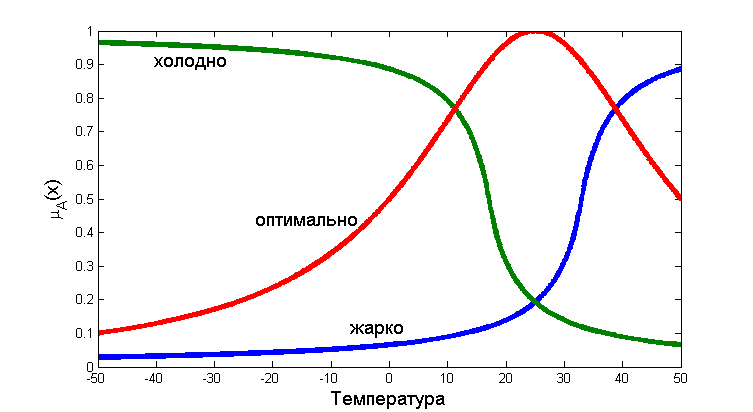
\includegraphics[width=0.8\textwidth]{fig/fuzzyTemperature}
    \caption{Аналитически заданные функции $\mu_A(x)$ для градаций температуры}
    \label{fig:fuz:fuzzyTemperature}
\end{figure} 


\section{Операции над нечеткими множествами}

Над нечеткими множествами $A,B$ выделяют следующие основные операции:
\begin{enumerate}
    \item Объединение $A\cup B$: $\mu_{A\cup B}(x)=\max[\mu_A(x),\mu_B(x)]$;
    \item Пересечение $A\cap B$: $\mu_{A\cap B}(x)=\min[\mu_A(x),\mu_B(x)]$
    \item Отрицание $\overline{A}$: $\mu_{\overline{A}}(x)=1-\mu_A(x)$;
    \item Вычитание $A\backslash B$: $\mu_{A\backslash B}(x)=\min[\mu_A(x), 1-\mu_B(x)]$;
    \item Концентрация $CON(A)$: $\mu_{CON(A)}(x)=[\mu_A(x)]^2$;
    \item Растяжение $DIL(A)$: $\mu_{DIL(A)}(x)=\sqrt{\mu_A(x)}$;
    \item Нормализация $NORM(A)$: $\mu_{NORM(A)}(x)=\frac{\mu_A(x)}{\sup\{\mu_A(y)|y\in U\}}$;
\end{enumerate}

Необходимо отметить, что в отличие от <<обычных>> множеств, одноименные операции не обладают теми же свойствами, в частности:
\begin{itemize}
    \item $A\cup\overline{A}\neq U$;
    \item $A\cap\overline{A}\neq\emptyset$.
\end{itemize}

$A\subseteq B$, если $\forall x\in U (\mu_A(x)\leq\mu_B(x))$. Для равенства: $A=B\Leftrightarrow (A\subseteq B)\land(B\subseteq A)$.

В нечеткой логике нечеткому множеству соответствует так называемая \emph{лингвистическая переменная}. И операции над нечеткими множествам соответствуют логическим связкам между лингвистическими переменными (см. рис. \ref{fig:fuz:fuzzyOperations}). Например, объединение соответствует связке <<ИЛИ>>, пересечение --- <<И>>, отрицание --- <<НЕ>>. Концентрация соответствует прилагательному <<ОЧЕНЬ>> перед лингвистической переменной, а растяжение --- прилагательным <<ПОЧТИ>>,<<ПРИМЕРНО>> (см. рис. \ref{fig:fuz:fuzzyConDil}).

\begin{figure}
    \centering
    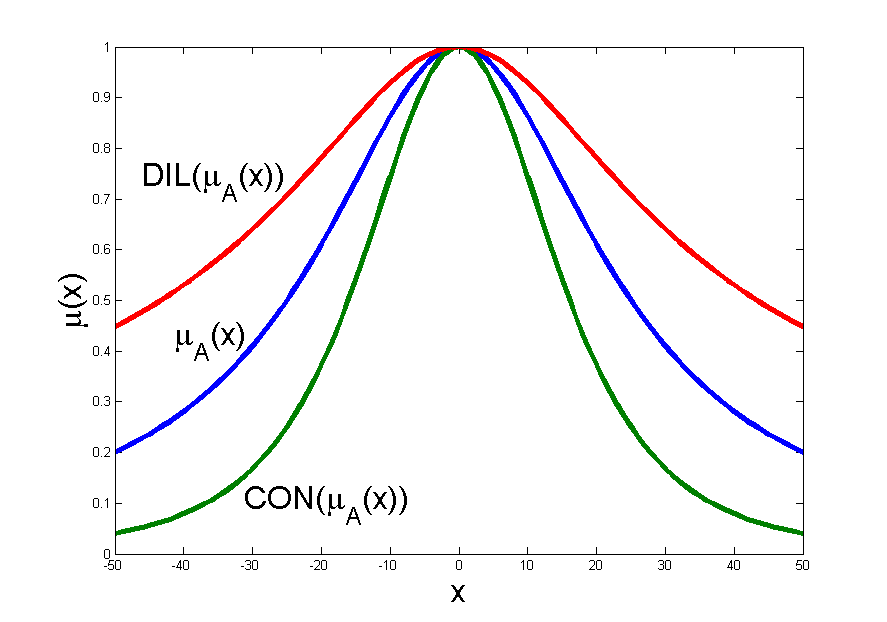
\includegraphics[width=0.8\textwidth]{fig/fuzzyConDil}
    \caption{Концентарция и растяжение нечёткого множества $A$}
    \label{fig:fuz:fuzzyConDil}
\end{figure} 


\begin{figure}
    \centering
    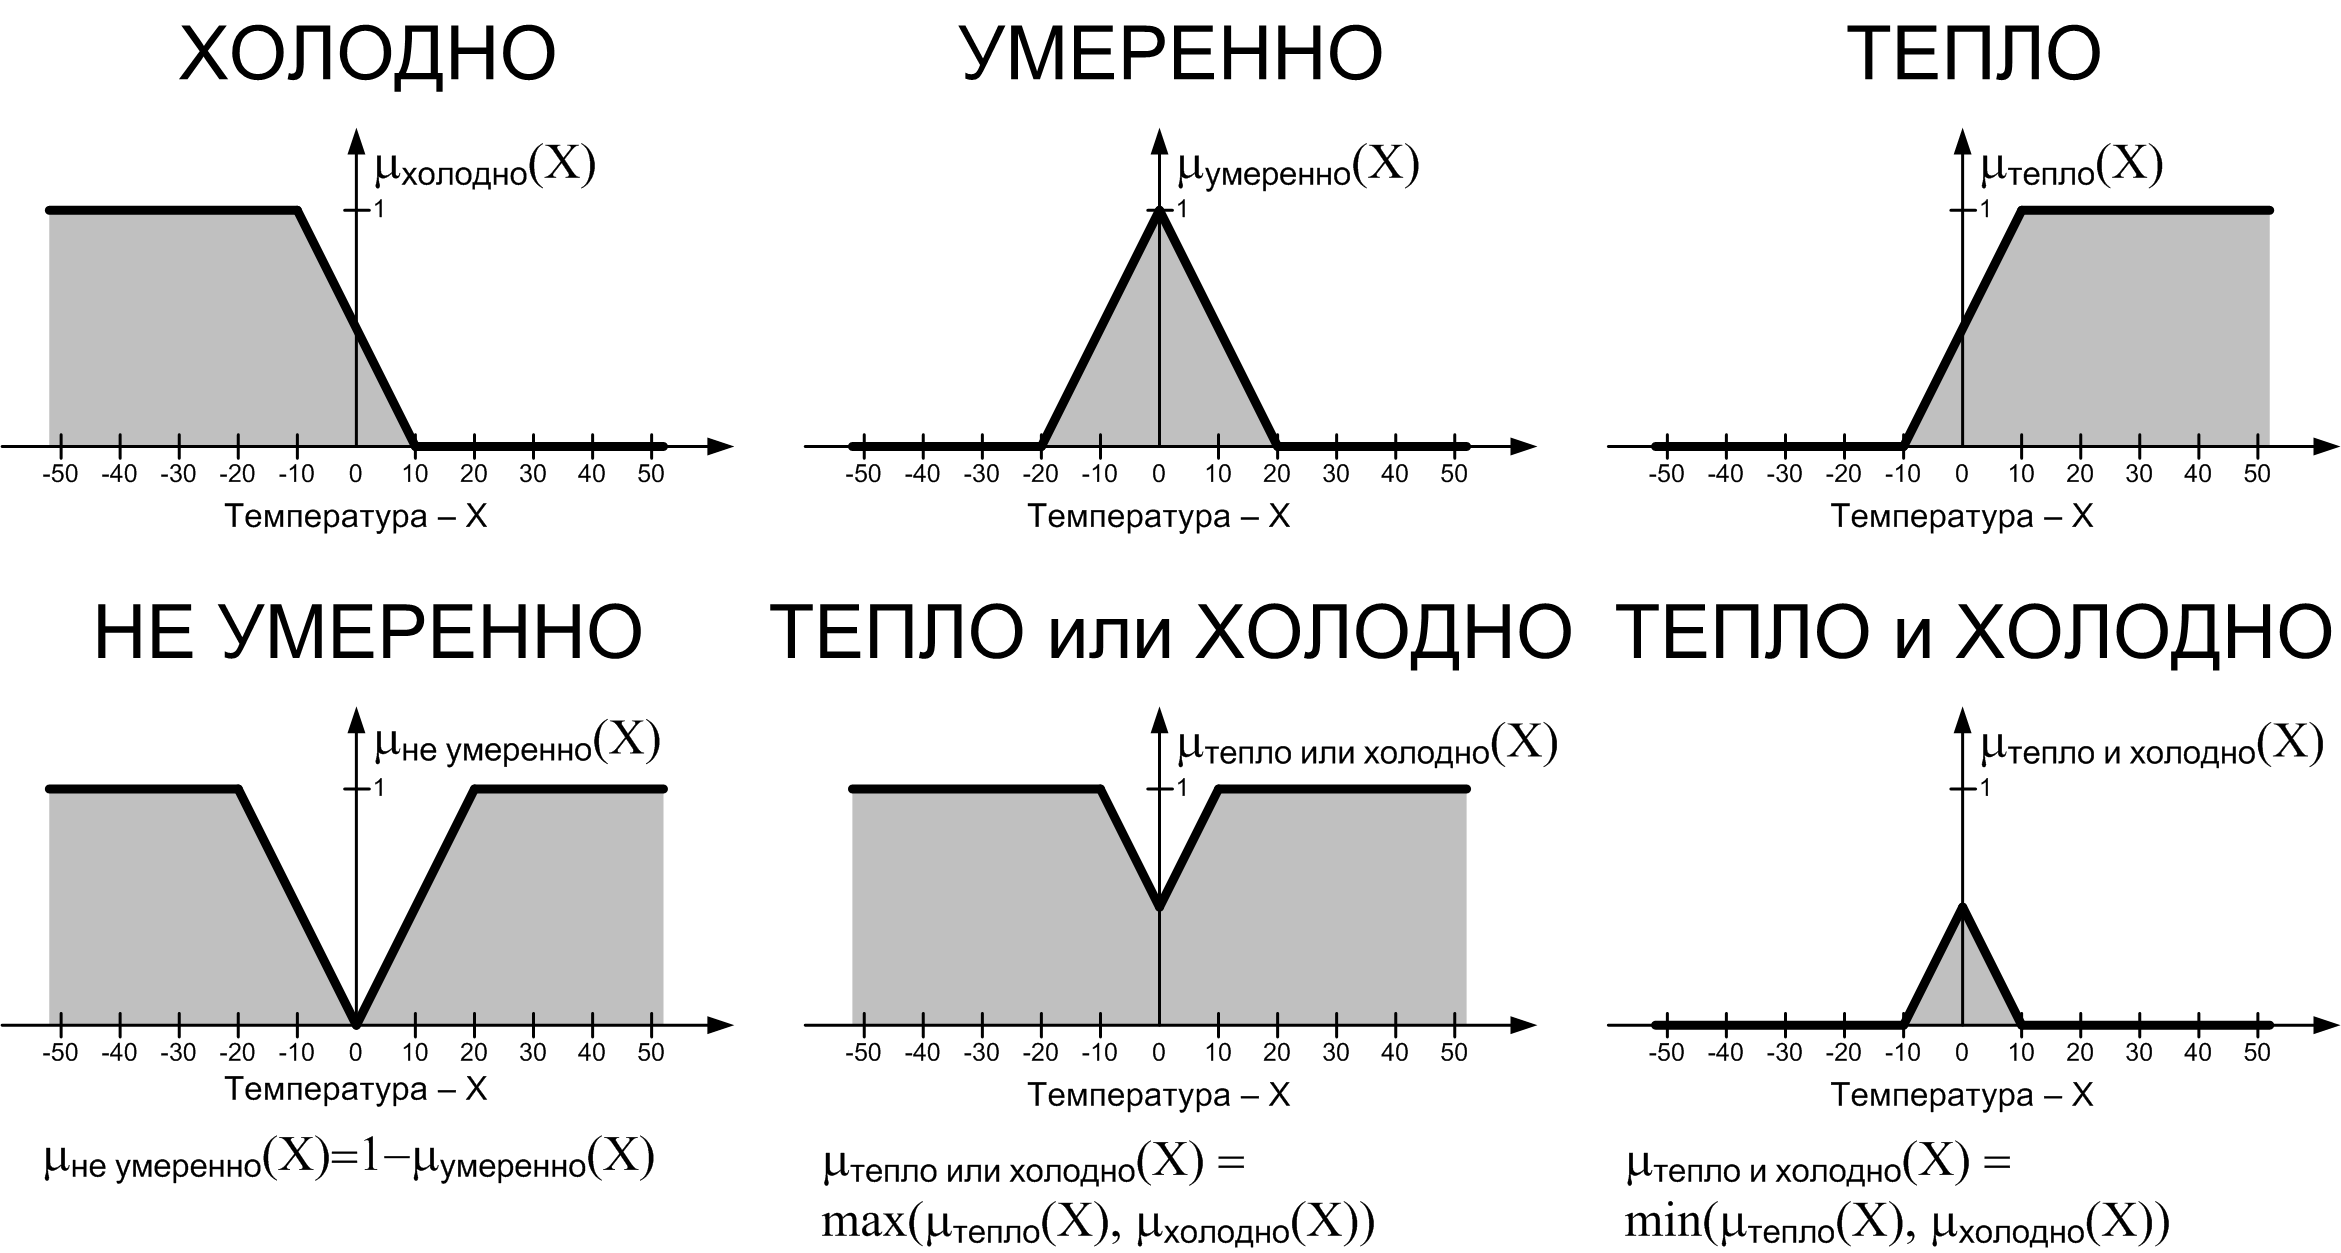
\includegraphics[width=0.9\textwidth]{fig/fuzzyOperations}
    \caption{Логические связки между лингвистическими переменными соответствуют операциям над нечеткими множествами}
    \label{fig:fuz:fuzzyOperations}
\end{figure} 

Видно, что бинарные операции основаны на функциях $\min$ и $\max$. В общем случае вместо $\min$ используют функцию $T:[0,1]\times[0,1]\to[0,1]$, которая называется \emph{$t$-нормой}, а вместо $\max$ используют функцию $S:[0,1]\times[0,1]\to[0,1]$, которая называется \emph{$t$-конормой}. $t$-норма обладает следующими свойствами:
\begin{enumerate}
    \item ограниченность: $T(0,0)=0,T(1,\mu)=\mu,T(\mu,1)=\mu$;
    \item монотонность: $T(\mu_1,\mu_2)\leq T(\mu_3,\mu_4)$, если $\mu_1\leq\mu_3, \mu_2\leq\mu_4$;
    \item коммутативность: $T(\mu_1,\mu_2)=T(\mu_2,\mu_2)$;
    \item ассоциативность: $T(\mu_1,T(\mu_2, \mu_3))=T(T(\mu_1,\mu_2),\mu_3)$;
\end{enumerate}

Примерами $t$-норм могут являться функции:
\begin{itemize}
    \item $T(\mu_1,\mu_2)=\min(\mu_1,\mu_2)$;
    \item $T(\mu_1,\mu_2)=\mu_1\cdot \mu_2$;
    \item $T(\mu_1,\mu_2)=\max[0,\mu_1+\mu_2-1]$.
\end{itemize}

$t$-конорма обладает следующими свойствами:
\begin{enumerate}
    \item ограниченность: $S(1,1)=1,S(0,\mu)=\mu,S(\mu,0)=\mu$;
    \item монотонность: $S(\mu_1,\mu_2)\geq S(\mu_3,\mu_4)$, если $\mu_1\geq\mu_3, \mu_2\geq\mu_4$;
    \item коммутативность: $S(\mu_1,\mu_2)=S(\mu_2,\mu_2)$;
    \item ассоциативность: $S(\mu_1,S(\mu_2, \mu_3))=S(S(\mu_1,\mu_2),\mu_3)$;
\end{enumerate}

Примерами $t$-конорм могут являться функции:
\begin{itemize}
    \item $S(\mu_1,\mu_2)=\max(\mu_1,\mu_2)$;
    \item $S(\mu_1,\mu_2)=\mu_1+\mu_2-\mu_1\cdot\mu_2$;
    \item $S(\mu_1,\mu_2)=\min[1,\mu_1+\mu_2]$.
\end{itemize}

Нечеткие множества лежат в основе нечеткой логики, рассмотрение которой выходит за рамки данного курса. Заинтересовавшимся практическим применением нечеких множеств можно рекомендовать \cite{bib:osovsky:neyro}.

\section*{Задания}
\addcontentsline{toc}{section}{Задания}

\begin{enumerate}
    
    \item Доказать, что $t$-конорма $T(\mu_1,\mu_2)=\mu_1+\mu_2-\mu_1\cdot\mu_2$ это функция $T:[0,1]\times[0,1]\to[0,1]$. Т.е. что $\rho_T=[0,1]$. Также доказать, что она ассоциативна.
    %a+b-ab = a(1-b)+b = a(1-b)+b-1+1 = a(1-b)-(1-b)+1 = 1-(1-a)(1-b)
    
    \item Докажите, что для нечеткого множества $A$ справедливо $A\subseteq DIL(A)$.
    
    \item Нечеткие множества на универсуме <<насекомое>> заданы в таблице \ref{table:fuz:insectos}. Найти нечеткое множество, соответствующее лингвистической переменной:
    \begin{enumerate}
        \item Опасно и не опасно
        \item Очень опасно
        \item Большое и не опасно
        \item Спутник и опасно
        \item Яркое и сильное
        \item (Яркое или большое) и не плодовитое
    \end{enumerate}

    Найдется ли среди представленных в таблице \ref{table:fuz:insectos} множество, являющееся подмножеством какого-либо другого множества.
    \begin{table}
        \centering
        \begin{tabular}{l||c|c|c|c|c|}
            Переменная&
                                \rotatebox{90}{Скорпион}&
                                        \rotatebox{90}{Пчела}&
                                                \rotatebox{90}{Шершень}&
                                                        \rotatebox{90}{Капустница}&
                                                                \rotatebox{90}{Муравей} \\
            \hline\hline
            Опасно(для человека)&0.5    &0.4    &0.5    &0.01   &0.1    \\ \hline
            Большое             &0.8    &0.2    &0.7    &0.6    &0.01   \\ \hline
            Яркое               &0.2    &0.1    &0.5    &0.5    &0.01   \\ \hline
            Сильное             &0.5    &0.3    &0.4    &0.01   &0.99   \\ \hline
            Плодовито           &0.1    &0.9    &0.1    &0.8    &0.9    \\ \hline
            Спутник(человека)   &0.1    &0.8    &0.2    &0.5    &0.1    \\ \hline
        \end{tabular}
        \caption{Лингвистические переменные на универсуме насекомых}
        \label{table:fuz:insectos}
    \end{table}

    \item Докажите справедлив ли закон дистрибутивности операций над нечеткими множествами $A\cap(B\cup C)=(A\cap B)\cup (A\cap C)$ и $A\cup(B\cap C)=(A\cup B)\cap (A\cup C)$, если в качестве пары ($t$-норма,$t$-конорма) выбрана пара:
    \begin{enumerate}
        \item $(\min,\max)$;
        \item $(\mu_1\cdot\mu_2,\mu_1+\mu_2-\mu_1\cdot\mu_2)$.
    \end{enumerate}
    
\end{enumerate}
 %Нечёткие множества
    \chapter{Основы кодирования}

%code: label prefix
Далее считается, что \emph{информация} --- это упорядоченная последовательность \emph{кодовых символов}, принадлежащих конечному алфавиту. Информация является своеобразным \emph{отражением} определенного \emph{события}. Оценить количество информации просто: это число кодовых символов последовательности. Сложнее оценить сколько информации несет событие, то есть последовательности какой длины достаточно для корректного отражения события. 

Клод Шеннон в 1948 г. определил оценку количества информации, которую несет событие так:
\begin{enumerate}
    \item Количество информации $I$ есть непрерывная функция от вероятности $p$ события. 
    \item Количество информации $I_i$ одиночного $i$-го события $s_i$, $s_i\in S$ ($S$ --- множество всех событий), $i\in[1,n]$ ($n$ --- количество различных событий в $S$), происходящего с вероятностью  $p_i$, имеет положительное значение $I_i\geq 0$;$I_i=I(p_i)$. Причем  $\sum_{i=1}^n p_i=1$.
    \item Совместное количество информации $I_{ij}$ двух независимых событий $s_i$,$s_j$ с совместной вероятностью $p_{ij}=p_i\cdot p_j$, равна сумме их количеств их информаций $I_{ij}=I_i+I_j$; $I(p_i\cdot p_j )=I(p_i )+I(p_j)$.
\end{enumerate}

\begin{exampl}
    Количество воспринимаемой информации влияет на эмоциональное состояние человека и постулаты Шеннона легко проверить на себе.
    
    Согласно Шеннону, количество информации зависит от вероятности наступления события. Сравните свои эмоции от двух событий: <<Жучка укусила Иванова>> и <<Иванов укусил Жучку>>. Первое событие, хоть собака и друг человека, будничное, а вот второе вызывает улыбку --- сенсация! Вероятность первого события весьма велика, вероятность второго близка к нулю. Первое событие несет мало информации, а второе несет большое её количество, отсюда и эмоции.

    В то же время, если мы на следующий день услышим, что после Иванова Жучку укусил еще и Петров, то внутренне мы будем готовы к тому, что на третий день Жучку укусит и Сидоров --- только ленивый не кусает Жучку! Хотя по правилам теории вероятности, с точки зрения обывателя, который не в курсе отношений Жучки с людьми, вероятность того, что Жучку укусит Иванов также мала, как и вероятность быть покусанной Петровым, и равна $p$. Вероятность, того, что Жучка будет покусана обоими, равна произведению вероятностей этих событий: $p^2$ --- это практически невероятно, так как $p^2$ много меньше $p$ и следует ожидать большой сенсации. Но! Никто (разве что Жучка) не падает в обморок от совместных действий Иванова и Петрова, так как количество информации, которое несет данное событие, есть лишь сумма количеств информаций для каждого факта оскорбления действием Жучки в отдельности.
    \qed
\end{exampl}

Постулатам Клода Шеннона удовлетворяет функция:
\begin{equation}
    \label{eq:code:shannon}
    I(p)=-\log_m p,
\end{equation}
где $p$ --- вероятность события, а $m$ количество кодовых символов в алфавите. При этом $m$ определяет единицы измерения информации. Например:
\begin{itemize}
    \item $m=2$: $[I]$ --- бит;
    \item $m=e$: $[I]$ --- нат;
    \item $m=3$: $[I]$ --- трит;
    \item $m=10$: $[I]$ --- дит.
\end{itemize}

Процесс сопоставления событиям информационных цепочек называется \emph{кодированием}.

Изложение  математических основ кодирования можно найти, например, в \cite{bib:novic:discrmathprogrammer,bib:yablonsky:discreteintro}. По основам теории информации можно рекомендовать книгу \cite{bib:panin:informationTheory}. Основы кодирования подробно изложены в \cite{bib:verner:codingBase}. Краткая теория приведена ниже.


\section{Назначение и формальное определение кодирования}

Можно выделить следующие основные назначения кодирования:
\begin{itemize}
    \item принципиальная возможность описания мира с помощью \emph{символов} конечного алфавита;
    \item устранение избыточности информации, её сжатие, и как следствие экономия памяти и снижение нагрузки на каналы передачи информации;
    \item защита информации (точнее защита таких свойств информации как: конфиденциальность, целостность, принадлежность, и т.д.).
\end{itemize}

Рассмотрим классическую задачу <<о картах>>:
\begin{exampl}
    \label{exampl:code:cards}
    Задача о картах. Имеется колода из восьми карт. По две карты (допустим, туз и двойка) каждой масти. Профессор вытягивает наугад карту и готов честно давать ответы да/нет на любые задаваемые вопросы. Нужно минимальным количеством вопросов угадать вытащенную карту.
\end{exampl}
\begin{proof}[Решение]
    Можно решить задачу задавая вопросы о конкретной карте. Тогда можно угадать карту с первого вопроса, но вероятность тому весьма мала. В худшем же случае, очевидно, потребуется семь вопросов.
    
    Более <<тонкое>> решение: каждым вопросом сокращать неопределенность вдвое. Например, ответ на первый вопрос о цвете масти разделит нам исходную колоду на две равные части по четыре карты. Вопрос о конкретной масти оставит нам две карты. И вопрос о достоинстве карты будет последним. 
    
    На рисунке \ref{fig:code:cards} ответам <<да>> соответствует символ $0$, а <<нет>> --- $1$. Продвигаясь от вершины дерева до конкретной карты поставим ей в соответствие получаемую цепочку символов. Эта цепочка символов и будет являться \emph{кодом} карты.
    
    \begin{figure}
        \centering
        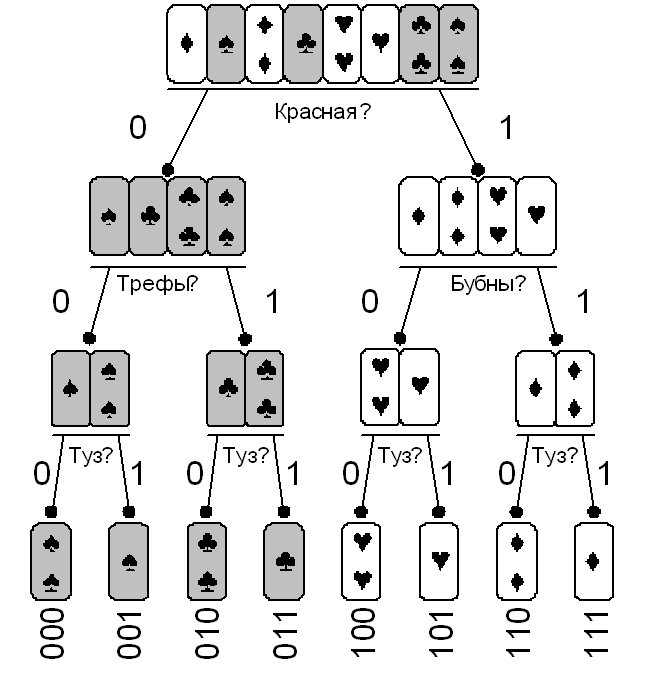
\includegraphics[width=0.47\textwidth]{fig/cards}
        \caption{Решение задачи о картах}
        \label{fig:code:cards}
    \end{figure}
    
    Теперь, договорившись с профессором о способе кодирования, можно попросить его так же честно сообщать \emph{код} вытащенной карты. И если он передал вам записанную на бумажке цепочку символов $011$, вы без труда догадаетесь, что из колоды был изъят туз треф.
\end{proof}

Полученную в процессе кодирования цепочку-информацию далее можно преобразовать в \emph{сигнал} и передавать по каналам связи. Так, например, непосредственный контакт с профессором из примера \ref{exampl:code:cards} больше не нужен: информация о карте может быть передана миганием фонарика, стуком, морзянкой по радио и т.д.

Не нужно забывать, что кроме \emph{бита} существуют и другие единицы измерения информации.
\begin{exampl}
    \label{exampl:code:femida}
    Задача о биллиардных шарах. Имеется восемь биллиардных шаров с номерами $1$-$8$ соответственно. Все шары одинаковой массы, кроме одного, который тяжелее остальных. Имеются весы Фемиды (чашечные). Какое количество взвешиваний вам потребуется, чтобы определить номер тяжелого шара?
\end{exampl}
\begin{proof}[Решение] 
    Весы Фемиды выдают информацию тритами, поэтому вам потребуется всего два вопроса. Коды шаров будут состоять из двух символов (см. рис. \ref{fig:code:femida}).
    \begin{figure}
        \centering
        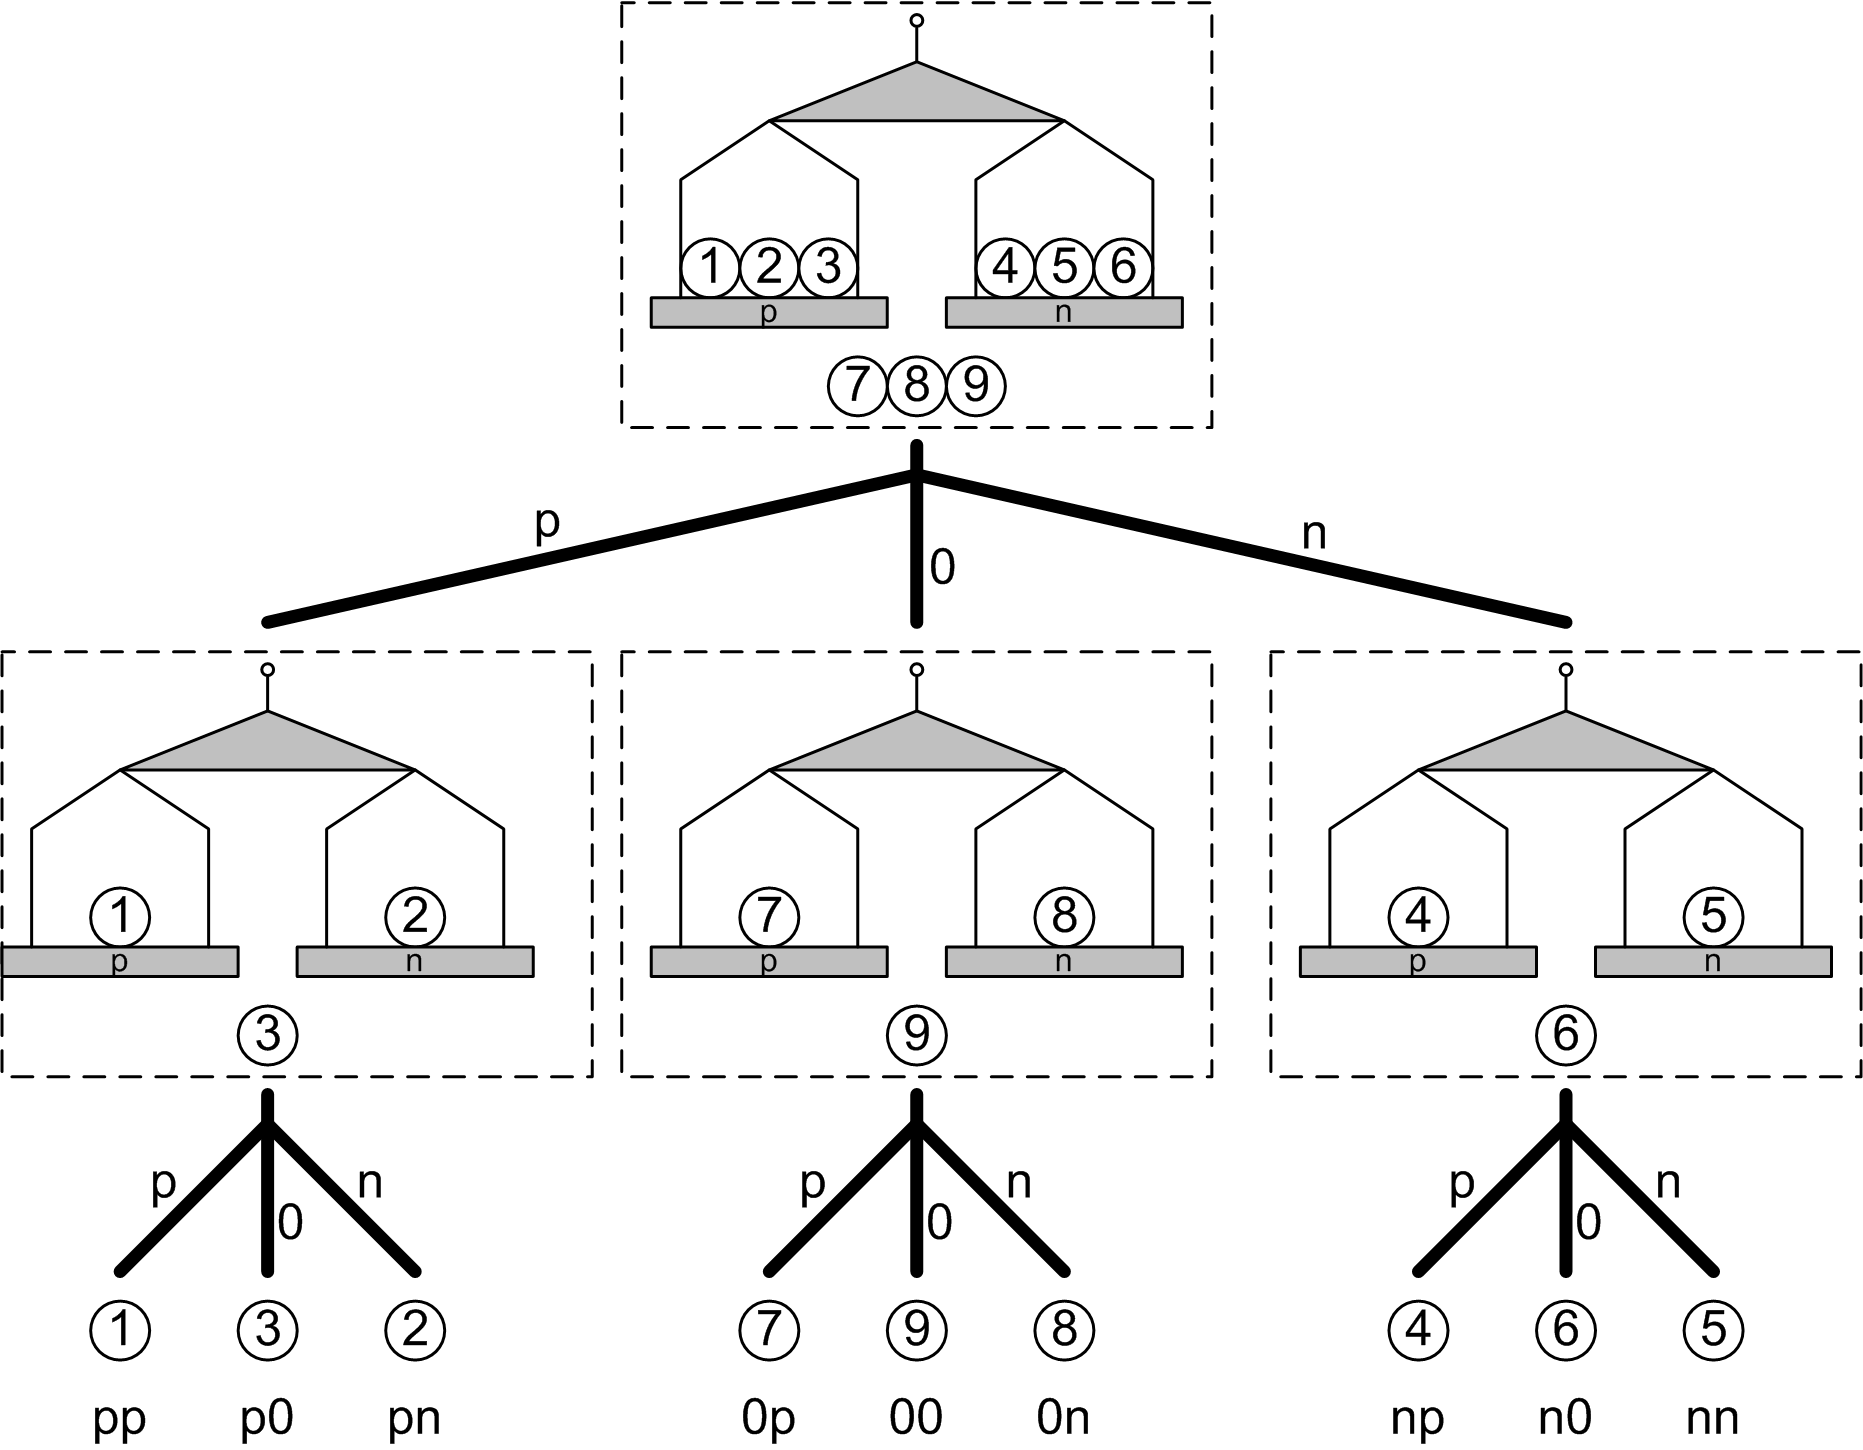
\includegraphics[width=0.47\textwidth]{fig/femida}
        \caption{Решение задачи о картах}
        \label{fig:code:femida}
    \end{figure}    
\end{proof}

Формально кодирование можно определить так. Имеется множество (алфавит) \emph{событий} 
\[
    S=\{s_1,\ldots,s_n\},
\] где $s_i$ --- буква алфавита событий (событие), $n$ --- количество событий (букв) алфавита $S$.

Алфавит \emph{кодовых символов}:
\[
    A=\{a_1,\ldots,a_m\},
\] где $a_i$ --- буква кодового алфавита (символ), а $m$ --- количество смволов в $A$. 

Требуется задать соответствие (схему, таблицу кодов) $\delta$ между событием $s_i$ и \emph{кодовым словом} $\omega_i=a_{i_1}\cdots a_{i_k}$:
\[
    \delta=\{ s_1\mapsto\omega_1, \ldots, s_n\mapsto\omega_n\}.
\]

Причем слово $\varsigma_j$, состоящее из букв алфавита $S$
\[
    \varsigma_j=s_{j_1}\cdots s_{j_t}
\]
будет кодироваться символами кодового алфавита как
\[
    \varsigma_j=\omega_{j_1} \cdots \omega_{j_t}.
\]
Множество кодовых слов $\omega_i$, соответствующих $s_i$ называется множеством \emph{элементарных кодов}:
\[
\Omega=\{\omega_1,\ldots,\omega_n\},
\]

\begin{exampl}
    Для кодирования \emph{букв} из множества $S=\{A,B,C,D,E,F,G,H\}$ с помощью \emph{слов} алфавита $A=\{0,1\}$ применяется следующее соответствие:
    \[
    \begin{split}
        \delta=\{ 
            A \mapsto 0,
            B \mapsto 1,
            C \mapsto 10,
            D \mapsto 11,
            E \mapsto 100,\\
            F \mapsto 101,
            G \mapsto 110,
            H \mapsto 111
        \}
    \end{split}
    \]

    Как видно, такое кодирование однозначно, но не взаимо однозначно. Слову $ABBA$ однозначно соответствует $0110$, а вот цепочке $0110$ соответствуют еще и
    \[AG\xrightarrow{\delta} 0110 \xleftarrow{\delta} ADA.\]

    Взаимно однозначный вариант кодирования может быть следующим:
    \[
        \begin{split}
            \delta=\{ 
                A \mapsto 000,
                B \mapsto 001,
                C \mapsto 010,
                D \mapsto 011,
                E \mapsto 100,\\
                F \mapsto 101,
                G \mapsto 110,
                H \mapsto 111
            \}
        \end{split}
    \]

    Теперь
    \[ABBA\xrightarrow{\delta} 000001001000\]
    декодируется однозначно.
    \qed
\end{exampl}

Таблица кодов $\delta$ является \emph{разделимой}, если любое слово $\varsigma_j$, составленное из элементарных кодов $\omega_i$ единственным образом разлагается на элементарные коды. При этом в таблице кодов не допускается, чтобы одному и тому же элементарному коду соответствовали различные буквы алфавита событий $s_i$.  Разделимая схема допускает \emph{декодирование}.

Важным частным случаем разделимых схем являются \emph{префиксные} схемы. Схема называется \emph{префиксной}, если ни один элементарный код $\omega_i$  из множества $\Omega$ не является префиксом другого кода из того же множества. \emph{Префиксом}, началом или приставкой слова $\omega$ называется слово $\omega_1$, если $\omega=\omega_1 \omega_2$. \emph{Постфиксом} или окончанием называется, соответственно, слово $\omega_2$. Коды, полученные на основе кодирующего дерева, см. например, рис. \ref{fig:code:cards}, очевидно, являются префиксными.

Наиболее простым вариантом кодирования является \emph{равномерное} кодирование, когда все элементарные коды одной длины. В этом случае требуется оценить длину цепочки кода, если количество кодируемых событий равняется $n$, а количество кодовых букв равняется $m$. Цепочкой из одного кодового символа можно закодировать $m$ событий, из двух --- $m^2$ и т.д. В общем случае из цепочкой из $I$ символов можно закодировать $m^I$ событий. Следовательно
\[
    I(n)=\lceil\log_m(n)\rceil,
\]
где $\lceil X \rceil$ --- наименьшее целое, большее или равное $X$.

Эту же оценку можно получить на основе постулатов Шеннона, предположив, что события равновероятны (т.е. вероятность любого события $p=\frac{1}{n}$). Тогда, в соответствии с формальным определением количества информации (см. формулу \eqref{eq:code:shannon}) для равномерного кодирования потребуется взять кодовые слова следующей длины:
\[
    I(n)=\lceil -\log_m\left(\frac{1}{n}\right)\rceil=\lceil \log_m(n) \rceil.
\]

Для приведенного примера с картами (пример \ref{exampl:code:cards}) длина кодов составляет $I(8)=\lceil \log_2(8) \rceil=3$ бита, а для примера (пример \ref{exampl:code:femida}) с весами Фемиды $I(8)=\lceil \log_3(8) \rceil=2$ трита.

\begin{exampl}
    В соревновании учавствуют $17$ спортсменов. Для регистрации пересечения финишной черты каждому спортсмену выдается радио-брелок. В момент пересечения финишной черты спортсменом, брелок передает двоичный код для идентификации спортсмена. Все брелки передают код одинаковой длины. Какое минимально необходиоме количество бит в общем случае должен передать брелок?
\end{exampl}
\begin{proof}[Решение] $\lceil \log_2(17)\rceil = 5$.
\end{proof}

В ряде случаев в процессе кодирования имеются знания о вероятности возникновения тех или иных событий. Если это так, то можно использовать методики оптимального кодирования для экономии памяти (или снижения нагрузки на каналы передачи данных).


\section{Оптимальное кодирование}

\emph{Источнику событий} после кодирования соответствует \emph{источник информации}, то есть источник, выдающий коды событий. Оценку информативности источника событий дает величина, называемая \emph{энтропией}:
\begin{equation}
    \label{eq:code:entrophyS}
    E=-\sum_{i=1}^n {p_i\cdot\log_m p_i},
\end{equation}
где $p_i$ --- вероятность $i$-го события $s_i\in S$ на выходе источника событий, $m$ --- количество информационных символов, используемых для кодирования, $n$ --- количество событий.

Так как вероятности появления кодов событий останутся прежними, то энтропия источника информации $E'$ будет равна
\begin{equation}
    \label{eq:code:entrophyI}
    E'=\sum_{i=1}^n {p_i\cdot I_i},
\end{equation}
где $I_i$ --- длина кода $\omega_i$ для $i$-го события .

Энтропия источника информации всегда больше энтропии отражаемого источника событий. Задача оптимального кодирования максимально приблизить энтропию источника информации к источнику событий.
\begin{exampl}
    Пусть имеется источник событий $s_i$, о вероятности появления которых на его выходе известно следующее:
    
    \begin{tabular}{|l|c|c|c|c|}
        \hline
        Событие $s_i$                   &А      &Б      &В      &Г   \\ \hline
        Вероятность $p_i$ события $s_i$ &0.5    &0.3    &0.1    &0.1 \\ \hline
    \end{tabular}
    
    Энтропия источника событий (формула \ref{eq:code:entrophyS}) составляет
    \[
        \begin{split}
            E=-(0.5\cdot\log_2 0.5+0.3\cdot\log_2 0.3+0.1\cdot log_2 0.1+0.1\cdot log_2 0.1)\approx \\
            \approx(0.5+0.521089678+0.332192809+0.332192809)\approx 1.685475297\text{\,бит}.
        \end{split}
    \]
    
    Для равномерного кодирования битами может быть получен такой вариант:

    \begin{tabular}{|l||c|c|c|c|}
        \hline
        Событие $s_i$                   &А      &Б      &В      &Г   \\ \hline
        Вероятность $p_i$ события $s_i$ &0.5    &0.3    &0.1    &0.1 \\ \hline
        Код события $\omega_i$          &00     &01     &10     &11  \\ \hline
    \end{tabular}
    
    Энтропия данного источника информации составит (формула \ref{eq:code:entrophyI})
    \[
        E'=(0.5\cdot 2+0.3\cdot 2+0.1\cdot 2+0.1\cdot 2)=2 \text{\,бита}.
    \]
    
    Видно, что энтропия источника информации значительно больше. Можно ли её уменьшить, приблизить к энтропии источника событий? Очевидно, что если кодировать символы с большей вероятностью появления кодом с меньшей длиной, то результаты должны получиться лучше. Попробуем следующую схему:
    
    \begin{tabular}{|l||c|c|c|c|}
        \hline
        Событие $s_i$                   &А      &Б      &В      &Г   \\ \hline
        Вероятность $p_i$ события $s_i$ &0.5    &0.3    &0.1    &0.1 \\ \hline
        Код события $\omega_i$          &0      &10     &110    &111 \\ \hline
    \end{tabular}
    
    Так же как и предыдущая, эта схема префиксная и разделимая, но неравномерная. Энтропия источника информации теперь составляет
    \[
        E'=(0.5\cdot 1+0.3\cdot 2+0.1\cdot 3+0.1\cdot 3)=1.7\text{\,бита}.
    \]
    Результаты много лучше! Так, если запустить источник информации на выдачу, например, $100$ кодов событий  то первый вариант кодирования выдаст нам цепочку длины примерно $200$, а второй примерно $170$ бит. Существенная экономия при том же качестве.
    \qed
\end{exampl}

Далее рассматриваются два алгоритма оптимального кодирования источника событий: алгоритм Хаффмана и алгоритм Фано. 
\paragraph{Алгоритм Хаффмана для $m=2$ (двоичное кодирование)}
\begin{enumerate}
    \item\label{enum:code:haffman2Sort} События сортируются по убыванию вероятности.
    
    \item\label{enum:code:haffman2Step} Два события с минимальными вероятностями объединяются в одно составное событие, которое имеет вероятность, равную сумме вероятностей исходных событий. При этом одно из исходных событий помечается кодовым символом $0$, а второе --- символом $1$. Исходные события исключаются из множества событий, вместо них остается одно составное. 
    
    \item Шаги \ref{enum:code:haffman2Sort} и \ref{enum:code:haffman2Step} последовательно повторяются до тех пор, пока все события не склеятся в единственное составное событие (корень), вероятность которого, очевидно, равна $1$. После этого кодовое слово $\omega_i$ для исходного события $s_i$ есть цепочка из кодовых символов, которыми помечены все составные события от  корня до $s_i$.
\end{enumerate}

\begin{exampl} Задача. С помощью алгоритма Хаффмана закодировать следующий источник событий.

    \begin{tabular}{|l||c|c|c|c|c|}
        \hline
        Событие $s_i$                   &А      &Б      &В      &Г      &Д      \\ \hline
        Вероятность $p_i$ события $s_i$ &0.5    &0.125  &0.125  &0.125  &0.125  \\ \hline
    \end{tabular}
\end{exampl}
\begin{proof}[Решение]
    Ход выполнения алгоритма Хаффмана отражен на рисунке \ref{fig:code:haffman2Ex}. После сортировки событий по убыванию вероятности видно, что вариантов для склеивания несколько. Произвольно выбираются два события с наименьшими вероятностями:Г и Д(энтропия от этого выбора не изменится). События Г и Д склеиваются в событие ГД с вероятностью $0.25$. Г помечается кодовым символом $0$, а Д --- $1$. Теперь множества событий выглядит так: \{А,Б,В,ГД\}. Наименьшую вероятность имеют события Б и В, которые и склеиваются в событие БВ с вероятностью $0.25$. Событие Б помечено символом $0$, а В --- $1$. Множество событий имеет вид {А,БВ,ГД}. Наименьшую вероятность имеют события БВ и ГД, которые и склеиваются в событие БВГД с вероятностью $0.5$. Событие БВ отмечено символом $0$, событие ГД символом $1$. Множество событий теперь имеет вид {А,БВГД}. Отмечая событие А символом $0$, а событие БВГД символом $1$, приходим к единственному событию в множестве событий {АБВГД} с вероятностью $1$.
    \begin{figure}
        \centering
        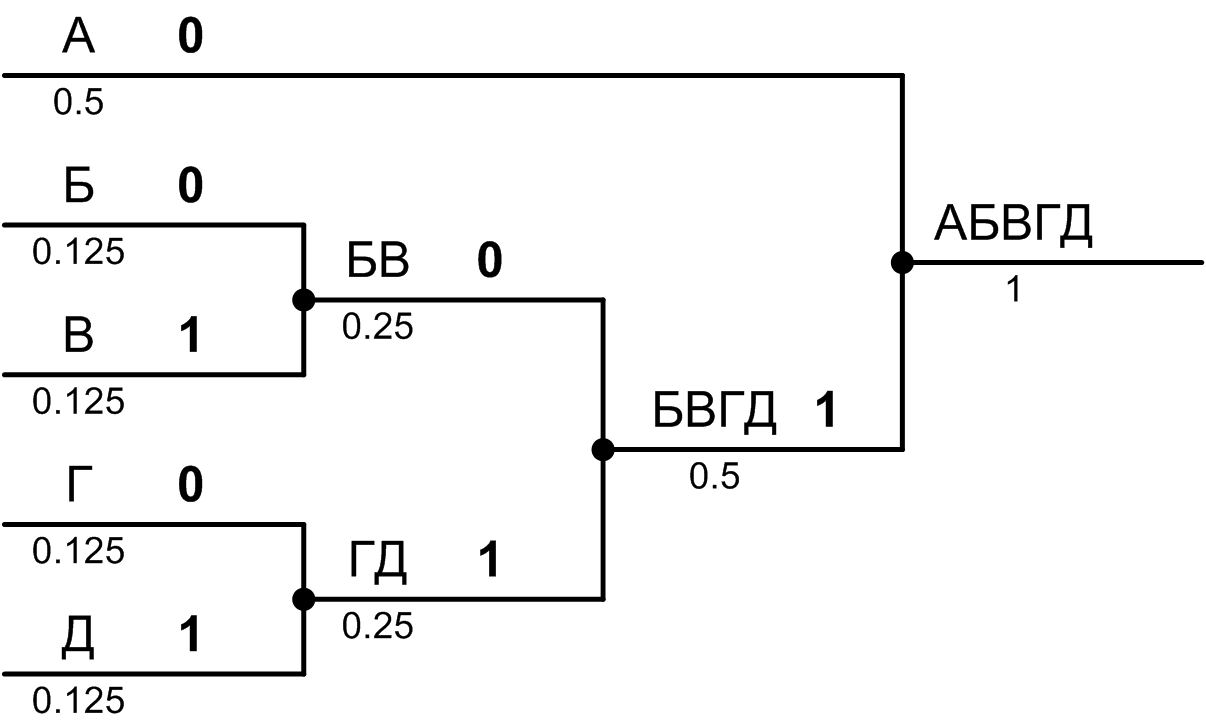
\includegraphics[width=0.6\textwidth]{fig/haffman2Ex}
        \caption{Кодирование источника по Хаффману}
        \label{fig:code:haffman2Ex}
    \end{figure} 
    Далее продвигаясь от корня (события АБВГД) до события исходного множества формируются кодовые слова $\omega_i$ из символов, которыми помечены промежуточные события на этом пути:
    \begin{tabular}{|l||c|c|c|c|c|}
        \hline
        Событие $s_i$                   &А      &Б      &В      &Г      &Д      \\ \hline
        Вероятность $p_i$ события $s_i$ &0.5    &0.125  &0.125  &0.125  &0.125  \\ \hline
        Код события $\omega_i$          &0      &100    &101    &110    &111    \\ \hline
    \end{tabular}
    
    Автоматически получен префиксный код. Попробуйте декодировать цепочку $10001101110111$.
\end{proof}

\paragraph{Алгоритм Фано для $m=2$}
\begin{itemize}
    \item[] На входе алгоритма имеется исходный массив событий, отсортированный в порядке убывания соответствующих им вероятностей (предполагается, что событий больше, чем $m$, иначе кодирование тривиально --- по одному символу на событие). Далее исходный массив разбивается на две части, так, чтобы разница сумм вероятностей событий каждой части была минимальна. Первый кодовый символ элементарного кода $\omega_i$ для каждого события $s_i$ находится так: для всех событий левой части разбитого массива первый кодовый символ будет $0$, а для всех событий правой части --- $1$. Второй и последующие кодовые символы определяется так: каждая часть разбитого исходного массива, в которой более одного события, становится исходным массивом, а разбиение с нахождением кодового символа для входящих в нее событий выполняется так же как для исходного массива.
\end{itemize}

\begin{exampl} Задача. С помощью алгоритма Фано закодировать следующий источник событий.

    \begin{tabular}{|l||c|c|c|c|c|c|c|c|}
        \hline
        $s_i$   &А      &Б      &В      &Г      &Д      &Е      &Ж      \\ \hline
        $p_i$   &0.135  &0.24   &0.25   &0.125  &0.0635 &0.124  &0.0625 \\ \hline
    \end{tabular}
\end{exampl}
\begin{proof}[Решение]
    Выполнение алгоритма Фано приводится в таблице \ref{table:code:fano}.
    \begin{table}
        \centering
        \begin{tabular}{|c|c||c|c|c|c|}
            \hline\hline
            $s_i$   &$p_i$  &\multicolumn{4}{c|}{$\omega_i$}\\ \hline\hline
            В       &0.25   &0&0&\multicolumn{2}{c|}{}      \\ \cline{4-4}
            Б       &0.24   &0&1&\multicolumn{2}{c|}{}      \\ \cline{3-5}
            А       &0.135  &1&0&0&                         \\ \cline{5-5}
            Г       &0.125  &1&0&1&                         \\ \cline{4-5}
            Е       &0.124  &1&1&0&                         \\ \cline{5-6}
            Д       &0.0635 &1&1&1&0                        \\ \cline{6-6}
            Ж       &0.0625 &1&1&1&1                        \\ \hline            
        \end{tabular}
        \caption{Выполнение алгоритма Фано}
        \label{table:code:fano}
    \end{table}
    
    На первом шаге найдем минимальную разницу сумм вероятностей среди вариантов разбиения на части: В:БАГЕДЖ=$|0.25-0.75|=0.5$; ВБ:АГЕДЖ=$|0.49-0.51|=0$.02; ВБА:ГЕДЖ=$|0.625-0.375|=0.25$; и т.д. очевидно, минимум это вариант ВБ:АГЕДЖ. Первый кодовый символ для событий части ВБ --- 0, для остальных событий части АГЕДЖ  --- 1. Имеем две части, для каждой из которых повторяется тот же алгоритм. Продолжим с частью АГЕДЖ, как с более интересной: А:ГЕДЖ=$|0.135-0.375|=0.24$; АГ:ЕДЖ=$|0.26-0.25|=0.01$; АГЕ:ДЖ=$|0.384-0.126|=0.258$; и т.д. минимум --- вариант АГ:ЕДЖ. Второй кодовый символ для событий АГ --- $0$, для событий ЕДЖ --- $1$. Для каждой части АГ и ЕДЖ повторяется тот же алгоритм. Например, для части АГ имеется единственный вариант разбиения А:Г и третий кодовый символ для А --- $0$, а для Г --- $1$. Так ни в одной части количество событий не превосходит единицы и делить уже нечего, то кодовые слова для событий А и Г определены. И так для всех получаемых частей.
\end{proof}


\section{Кодирование с целью сжатия информации}

Следует выделить различия между между \emph{оптимальным кодированием} и \emph{кодированием с целью сжатия}? Оптимальное кодирование ставит себе в задачу сопоставить источнику событий минимальное количество адекватной ему информации. Кодирование с целью сжатия ставит себе в задачу уменьшить количество информации, не теряя (или оставаясь в допустимых рамках) при этом свойство адекватности. Кодирование с целью сжатия будем далее называть просто \emph{сжатие}. В случае сжатия события $s_i$ уже представляют собой слова в алфавите $A$. То есть информация \emph{перекодируется} в том же алфавите $A$.

Выделяют два больших класса алгоритмов сжатия информации: сжатие с потерями и без потерь. Теряется, данном случае, конечно, адекватность отражения. При сжатии без потерь из сжатой информации можно восстановить исходную информацию в точности такую же, как до сжатия. При сжатии с потерями восстановленная информация будет отличаться от исходной. Ярким примером сжатия с потерями является сжатие изображений: используя определенные особенности восприятия цвета человеком, такие алгоритмы отбрасывают <<лишнюю>> информацию. Потеря адекватности отражаемому объекту в этом случае значительная, но для человека-потребителя эти потери адекватности незаметны.

Часто алгоритмы сжатия весьма специфичны и учитывают особенности отражаемого источника событий. Одним из важнейших таких источников в жизни человека является речь. Письмо --- способ кодирования речи с помощью символов конечного алфавита --- азбуки. На основе, например, русского алфавита можно построить бесконечное количество слов, но в реальной жизни словарный запас редко превышает сотню тысяч слов. На практике для универсального представления текста байтами кодируются буквы, цифры, знаки препинания, пробелы и т.д., но если мы знаем, что кодируется именно осмысленный текст (содержащий осмысленные слова), то можно сильно сэкономить, кодируя в качестве сообщений $s_i$ не буквы, а слова. Такие методы сжатия называются \emph{словарными}. 

Впрочем, словарные методы могут использоваться не только для кодирования текста, но для произвольных информационных цепочек. Причем словарь может строиться динамически и совершенно не учитывать смысловой нагрузки слов в словаре.

Далее будет рассмотрен алгоритм Лемпела-Зива, относящийся к группе словарных. В основе алгоритма Лемпела-Зива лежит идея \emph{адаптивного} сжатия: за один проход по цепочке одновременно строится и словарь и код, причем словарь не хранится, так как при декодировании он динамически восстанавливается.

\paragraph{Алгоритм Лемпела-Зива}
\begin{itemize}
	\item Кодирование
	\begin{enumerate}
		\item В словарь нулевым элементом помещается пустая цепочка $\varepsilon$. Пустое слово $\varepsilon$ не содержит букв и для любого слова $\omega$ справедливо $\omega=\varepsilon\omega=\omega\varepsilon$.
        
        \item\label{enum:code:lzWord} От исходной цепочки $t$ отделяется слово $\omega a$, где $\omega$ --- максимально длинное слово из словаря, $a$ --- расширяющая буква. Т.е. $t=\omega at'$.
        
        \item\label{enum:code:lzDict} В конец словаря добавляется новое слово $\omega a$. К коду c добавляется пара $\langle i_{\omega},a\rangle$, где $i_{\omega}$ --- индекс слова $\omega$ в словаре. От исходного текста отделяется слово $\omega a$: $t=t'$.
        
        \item Пункты \ref{enum:code:lzWord}-\ref{enum:code:lzDict} последовательно повторяются до тех пор, пока в тексте $t$ остается хоть одна буква.
	\end{enumerate}
    В результате получается код $c=\langle i_1,a_1\rangle\cdots\langle i_n,a_n\rangle$.
    
	\item Декодирование
    \begin{enumerate}
        \item В словарь нулевым элементом помещается пустая цепочка $\varepsilon$. Текст $t$ не содержит букв: $t=\varepsilon$.
        
        \item\label{enum:code:lzDecode} От исходного кода c отделяется пара $\langle i,a\rangle$, в словарь добавляется слово $\omega_i a$, где $\omega_i$ --- $i$-е слово из словаря (словарь восстанавливается так же, как и формируется!). Восстанавливается текст $t=t\omega_i a$.
        
        \item Пункт \ref{enum:code:lzDecode} последовательно повторяется до тех пор, пока в коде $c$ остается хоть одна пара.
    \end{enumerate}
\end{itemize}

Нужно отметить, что данный алгоритм хорошо сжимает тексты большого объема, в которых так или иначе будут присутствовать одинаковые и достаточно длинные слова. В следующем примере такие вхождения были созданы искусственно.

\begin{exampl} 
    Задача. Сжать текст <<АБАКАНКАНКАНКИАНКИН>>. Оценить выигрыш от сжатия. Восстановить текст из кода.
\end{exampl}
\begin{proof}[Решение]
    Процесс кодирования отражен в таблице \ref{t:code:lzEncodeEx}. Процесс декодирования в таблице \ref{t:code:lzDecodeEx}. Если предположить, что символы текста кодируются байтом, а каждая пара кода $\langle i,a \rangle$ двумя байтами (байт на индекс $i$, второй на букву $a$), то в данном случае объем текста $19$ байт, а кода --- $16$. Коэффициент сжатия $\frac{19}{16}$.
    \begin{table}
        \centering
        \begin{tabular}[c]{|l|l|l|l|}
            \hline\hline
            $i$ & $t$                                            & $\omega a$                         & $c=\langle i_\omega,a\rangle$ \\ 
            \hline\hline
              &                                                  & $0\mapsto\varepsilon $   & \\ \hline
            1 &	$\varepsilon\text{\textbf{А}БАКАНКАНКАНКИАНКИН}$ & $1\mapsto\text{A}    $   & $\langle\text{0,А}\rangle$ \\ \hline
            2 &	$\varepsilon\text{\textbf{Б}АКАНКАНКАНКИАНКИН} $ & $2\mapsto\text{Б}    $   & $\langle\text{0,Б}\rangle$ \\ \hline
            3 &	$           \text{\textbf{АК}АНКАНКАНКИАНКИН}  $ & $3\mapsto\text{АК}   $   & $\langle\text{1,К}\rangle$ \\ \hline
            4 &	$           \text{\textbf{АН}КАНКАНКИАНКИН}    $ & $4\mapsto\text{АН}   $   & $\langle\text{1,Н}\rangle$ \\ \hline
            5 &	$\varepsilon\text{\textbf{К}АНКАНКИАНКИН}      $ & $5\mapsto\text{К}    $   & $\langle\text{0,К}\rangle$ \\ \hline
            6 &	$           \text{\textbf{АНК}АНКИАНКИН}       $ & $6\mapsto\text{АНК}  $   & $\langle\text{4,К}\rangle$ \\ \hline
            7 &	$           \text{\textbf{АНКИ}АНКИН}          $ & $7\mapsto\text{АНКИ} $   & $\langle\text{6,И}\rangle$ \\ \hline
            8 &	$           \text{\textbf{АНКИН}}              $ & $8\mapsto\text{АНКИН}$   & $\langle\text{7,Н}\rangle$ \\ \hline
        \end{tabular}
        \caption{Сжатие:<<АБАКАНКАНКАНКИАНКИН>>}
        \label{t:code:lzEncodeEx}
    \end{table}
    \begin{table}
        \centering
        \begin{tabular}[c]{|l|l|l|l|}
            \hline\hline
            $i$ & $c=\langle i_\omega,a\rangle$ & $\omega a$                         & $t$ \\ 
            \hline\hline
              &                            & $0\mapsto\varepsilon $   &                                                 \\ \hline
            1 & $\langle\text{0,А}\rangle$ & $1\mapsto\text{A}    $   &	$\text{}      \varepsilon\text{\textbf{А}}    $ \\ \hline
            2 & $\langle\text{0,Б}\rangle$ & $2\mapsto\text{Б}    $   &	$\text{А}     \varepsilon\text{\textbf{Б}}    $ \\ \hline
            3 & $\langle\text{1,К}\rangle$ & $3\mapsto\text{АК}   $   &	$\text{АБ}               \text{\textbf{АК}}   $ \\ \hline
            4 & $\langle\text{1,Н}\rangle$ & $4\mapsto\text{АН}   $   &	$\text{АБАК}             \text{\textbf{АН}}   $ \\ \hline
            5 & $\langle\text{0,К}\rangle$ & $5\mapsto\text{К}    $   &	$\text{АБАКАН}\varepsilon\text{\textbf{К}}    $ \\ \hline
            6 & $\langle\text{4,К}\rangle$ & $6\mapsto\text{АНК}  $   &	$\text{АБАКАНК}          \text{\textbf{АНК}}  $ \\ \hline
            7 & $\langle\text{6,И}\rangle$ & $7\mapsto\text{АНКИ} $   &	$\text{АБАКАНКАНК}       \text{\textbf{АНКИ}} $ \\ \hline
            8 & $\langle\text{7,Н}\rangle$ & $8\mapsto\text{АНКИН}$   &	$\text{АБАКАНКАНКАНКИ}   \text{\textbf{АНКИН}}$ \\ \hline
        \end{tabular}
        \caption{Декодирование:<<0А0Б1К1Н0К4К6И7Н>>}
        \label{t:code:lzDecodeEx}
    \end{table}
\end{proof}
    
Качество сжатия словарными методами можно улучшить за счет начальной инициализации словаря. Заинтересовавшимся алгоритмами сжатия можно рекомендовать книгу \cite{bib:salmon:compressing}.


\section{Кодирование с целью защиты свойств информации}

Информация имеет несколько свойств, важных с точки зрения их защиты: \emph{целостность}, \emph{конфиденциальность}, \emph{принадлежность} и \emph{доступность}. Далее рассматриваются лишь методы кодирования с целью защиты целостности информации. \emph{Целостность} --- это неизменность информации относительно некоторого фиксированного значения. Защита этого свойства дает пользователю уверенность в том, что информация, полученная им по каналу связи, доставлена в том виде, в котором была отправлена.

Ошибки, возникающие в цифровом (двоичном) канале могут быть следующими:
\begin{itemize}
    \item замещения кодового символа;
    \item вставка кодового символа;
    \item выпадение кодового символа.
\end{itemize}

Далее рассматриваются только ошибки замещения. Существуют две стратегии использования вводимой информационной избыточности:
\begin{enumerate}
    \item с обнаружением ошибок и с последующим запросом на повторную передачу (ARQ --- Automatic Repeat Request);
    
    \item с непосредственным обнаружением и исправлением ошибок на стороне получателя (FEC --- Forvard Error Correction).
\end{enumerate}

Примером стратегии ARQ может считаться контроль по четности (нечетности). К исходному двоичному слову добавляется служебный бит информации (бит чётности $p_{\text{чётн}}$), содержащий сумму <<по модулю два>> (по исключающему или) всех бит исходного слова. Сложение по <<исключающему или>> (еще гворят по xor, по<<модулю два>>) ($\oplus$) выполняется по правилам:
\[
    \begin{array}[c]{||c||c|c|}
        \hline\hline
        \oplus  & 0 & 1\\ \hline\hline
        0       & 0 & 1\\ \hline
        1       & 1 & 0\\ \hline
    \end{array}
\]

Бит четности равен нулю только в том случае, если количество единичных бит слова чётно. Также используют контроль по нечётности, при этом значение бита нечетности $p_{\text{нечётн}}$ противоположно значению бита четности. То есть для $n$-разрядного слова $d_{n-1}\cdots d_1d_0$ получим:
\[
    \begin{split}
        p_{\text{чётн}}=d_{n-1}\oplus\ldots\oplus d_1\oplus d_0,\\
        p_{\text{нечётн}}=d_{n-1}\oplus\ldots\oplus d_1\oplus d_0\oplus 1.
    \end{split}
\]

Если рассчитанный по той же формуле бит не совпадает с переданным --- в канале произошла ошибка, требуется повторная передача. Ошибки четной кратности не данным кодом не распознаются.

Стратегия FEC позволяет не только выявлять ошибки, но и исправлять их на месте. Рассмотрим несколько примеров кодирования для исправления одиночной ошибки.

Можно кодировать каждый бит исходной последовательности по схеме
\[\delta=\{0\mapsto 000,1\mapsto 111\},\]
а декодировать по схеме
\[
    \begin{split}
        \delta'=\{
            000\mapsto 0,001\mapsto 0,010\mapsto 0,100\mapsto 0,\\
            111\mapsto 1,110\mapsto 1,101\mapsto 1,011\mapsto 1
        \},
    \end{split}
\]

\begin{exampl}
Пусть передается слово $101$. Кодируется $111000111$. Поступает в канал. Возникает одиночная ошибка: $11\fbox{$0$}000111$. Декодируется: $101$. При этом декодер обнаруживает и исправляет одиночную ошибку. \qed
\end{exampl}

Данный способ кодирования увеличивает нагрузку на канал связи в три раза. Это неприемлемо. Рассмотрим код Хемминга, дающий гораздо более экономичный результат. Код Хемминга формирует номер ошибочного разряда. Признаком отсутствия ошибок будет нулевой номер. Поэтому введем <<фиктивный>> нулевой разряд. Пусть исходное слово имеет длину $n$ бит, тогда к нему нужно добавить $m$ дополнительных бит, исходя из неравенства
\begin{equation}
    \label{eq:code:hammingM}
    2^m\geq n + m + 1,
\end{equation}
где левая часть неравенства --- это количество $m$-разрядных двоичных чисел, а правая --- общая длина кода с учетом <<фиктивного>> разряда. Выбирается минимальное $m$ из возможных.

\paragraph{Алгоритм построения кода Хемминга}
\begin{enumerate}
    \item В двоичном числе длиной $m+n$ бит (без фиктивного разряда) контрольные $m$ бит следует разместить в разрядах с номерами, равными степени двойки ($2^i,0\leq i<m$). А $n$ бит исходного слова следует разместить в оставшихся разрядах. Контрольный биты при этом инициализируются нулевыми значениями.
    
    \item\label{en:code:hammingCount} Каждый контрольный бит $c_{2^i}$ в разряде $2^i$ пересчитывается как сумма <<по модулю два>> бит кода, находящихся в разрядах с номерами, двоичное представление которых содержит единицу в $i$ разряде (включая и сам контрольный разряд).
\end{enumerate}

При декодировании контрольные разряды пересчитываются в соответствии с пунктом \ref{en:code:hammingCount} алгоритма построения кода. В результате в контрольных разрядах будет получено число --- двоичное представление номера разряда ошибочного бита.

\begin{exampl}
    Задача. Построить код Хемминга для слова $u=0011$.
\end{exampl}
\begin{proof}[Решение]
    $n=4$. Выбираем $m=3$, исходя из формулы \eqref{eq:code:hammingM}. Процесс кодирования представлен на рисунке \ref{fig:code:hammingEncode}. 
    \begin{figure}
        \centering
        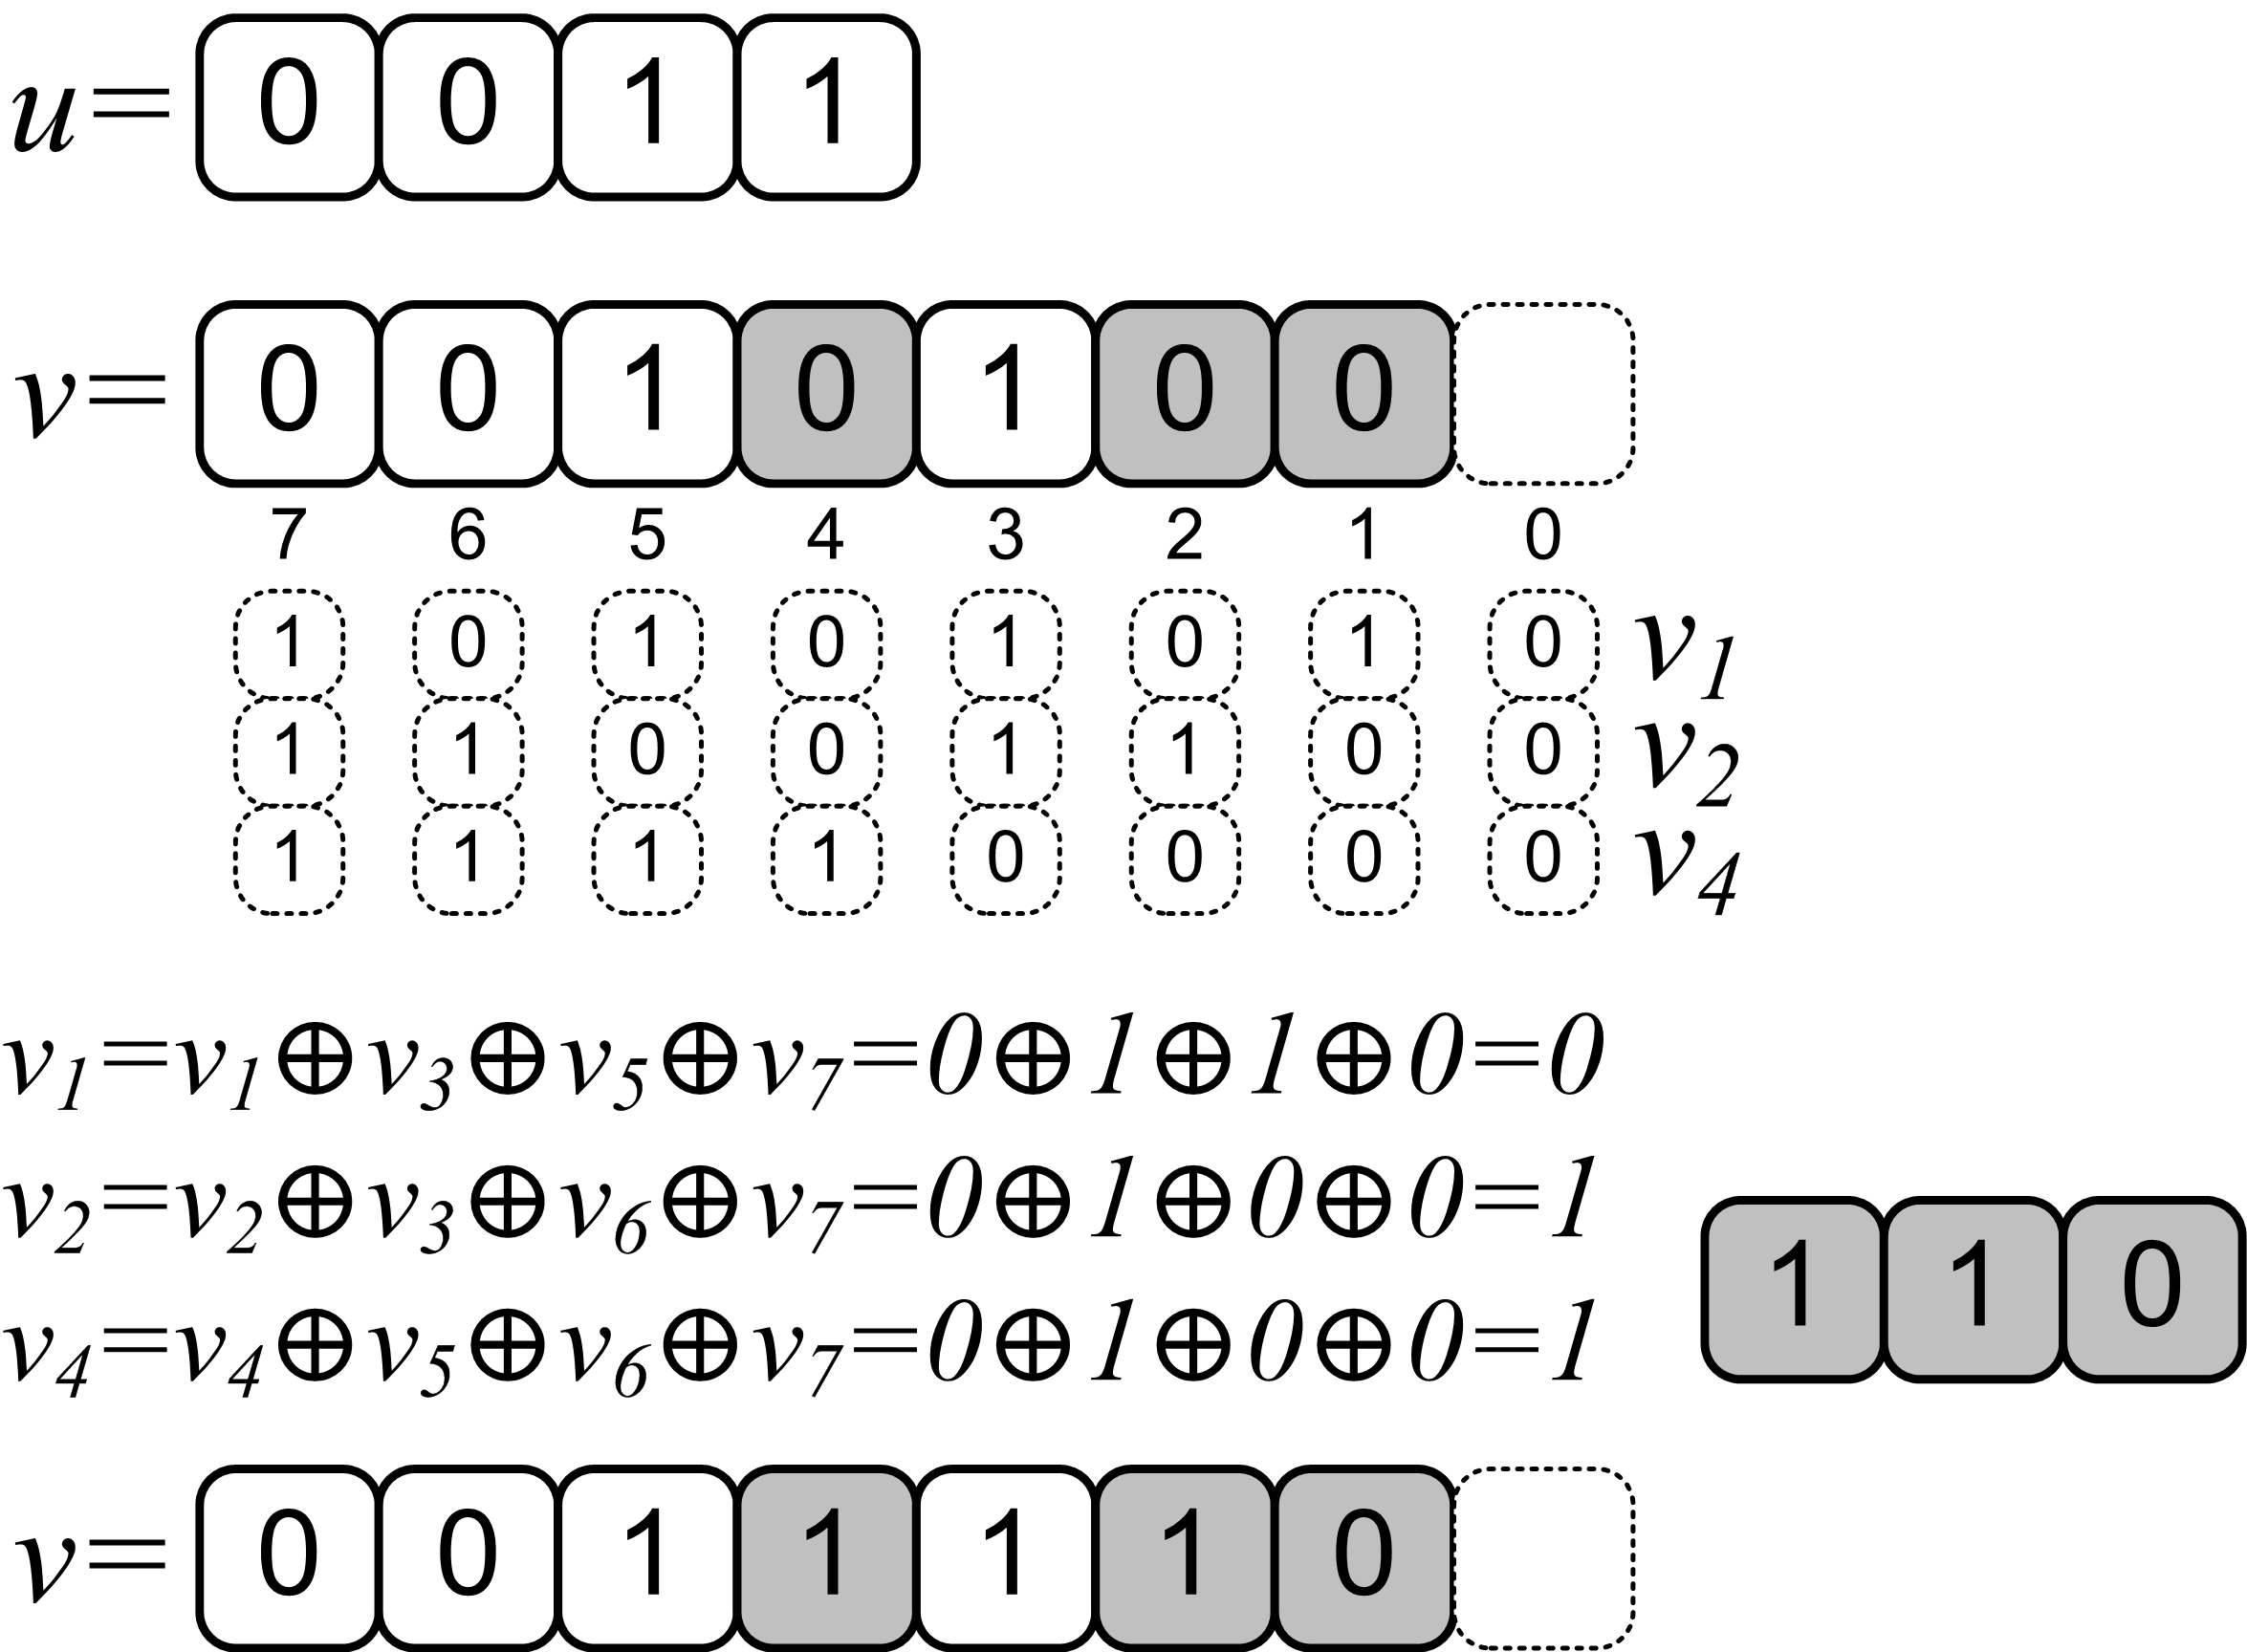
\includegraphics[width=0.6\textwidth]{fig/hammingEncode}
        \caption{Формирование код Хемминга}
        \label{fig:code:hammingEncode}
    \end{figure}
    \begin{figure}
        \centering
        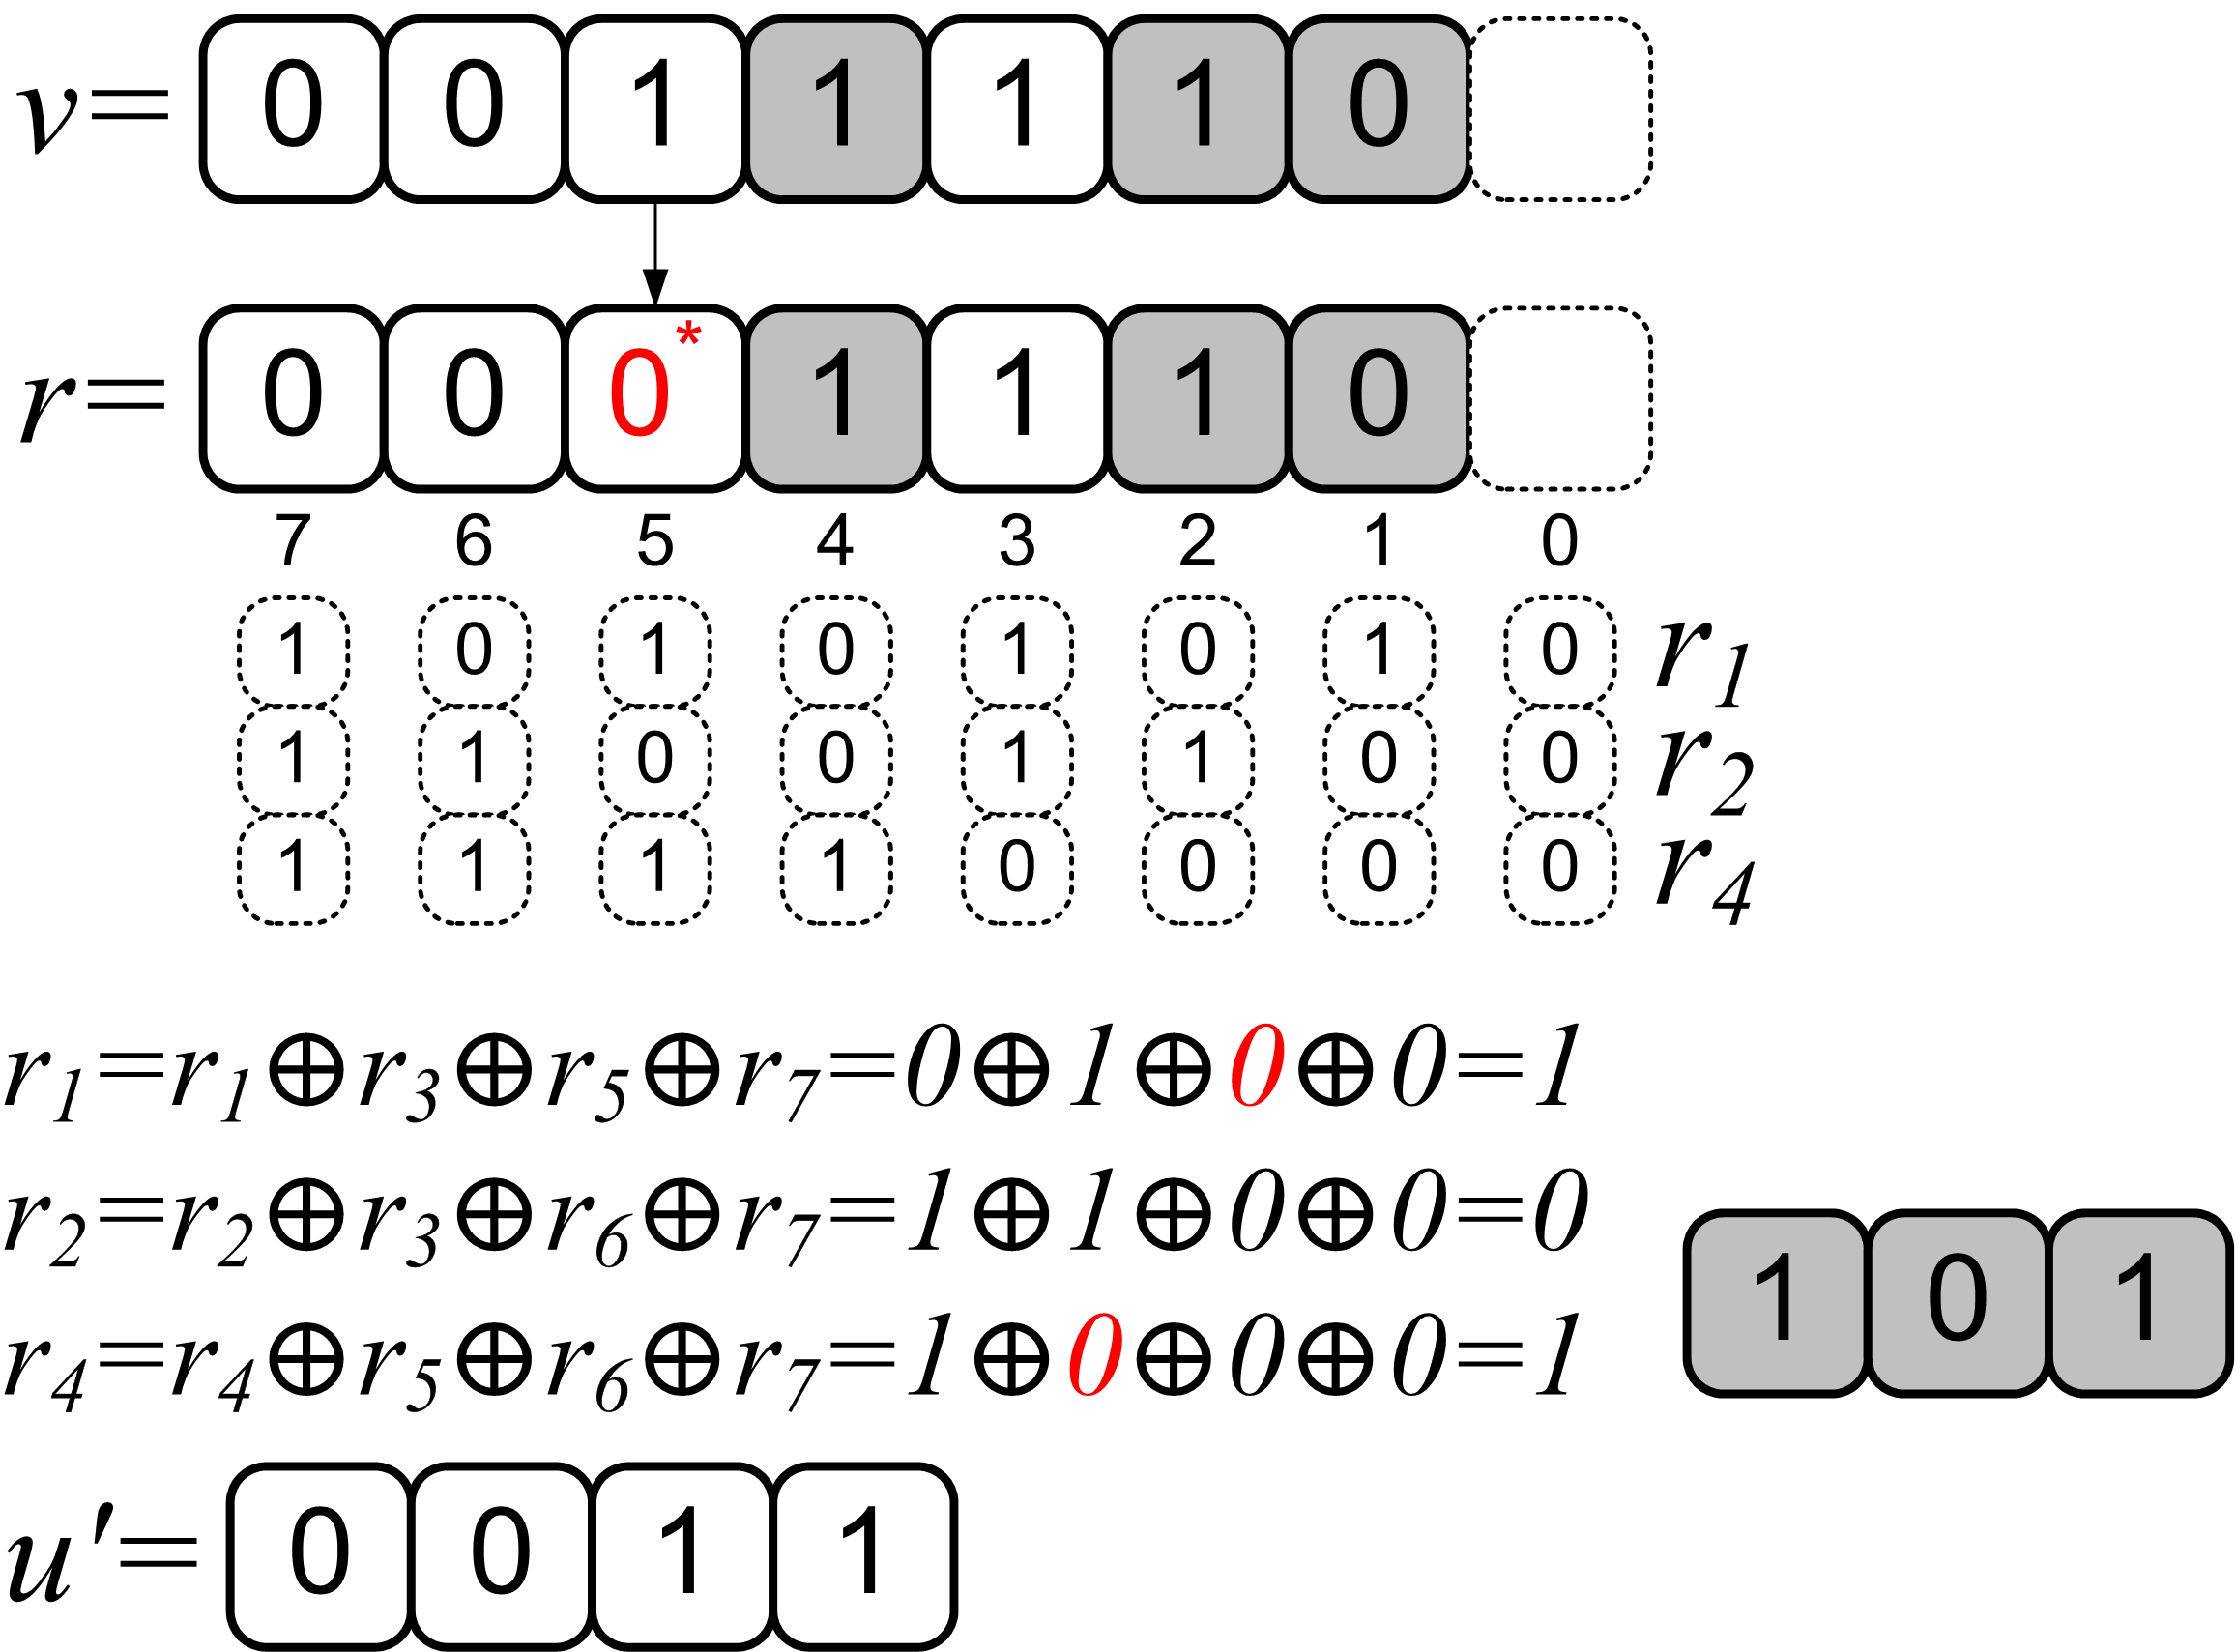
\includegraphics[width=0.6\textwidth]{fig/hammingDecode}
        \caption{Коррекция ошибки в коде Хемминга}
        \label{fig:code:hammingDecode}
    \end{figure}
    
    В результате получается код $v$. В ходе передачи происходит ошибка: пятый бит инвертируется, и пользователь принимает код $r$. Декодирование представлено на рисунке \ref{fig:code:hammingDecode}. В результате в контрольных разрядах формируется номер ошибочного бита, который инвертируется и извлекается исходный код $u'$. Код корректно исправляет одиночные ошибки и обнаруживает двойные, но может не обнаружить ошибки большей кратности.
\end{proof}


\section*{Задания}
\addcontentsline{toc}{section}{Задания}

\begin{enumerate}

    \item Множество кодовых символов $A=\{0,1\}$. Является ли приведенное ниже кодирование однозначным? Взаимно однозначным? Возможно ли декодирование? Код является префиксным? Разделима ли схема? Приведите контрпримеры, если необходимо.
    \begin{enumerate}
        \item $S=\{A,B,C,D\}$, $\delta=\{ A\mapsto 0,B\mapsto 11,C\mapsto 101, D\mapsto 110\}$;
        \item $S=\{A,B\}$, $\delta=\{ A\mapsto 0,B\mapsto 01\}$;
        \item $S=\{A,B,C\}$, $\delta=\{ A\mapsto 0,B\mapsto 01,C\mapsto 11\}$;
        \item $S=\{A,B,C,D\}$, $\delta=\{ A\mapsto 1,B\mapsto 01,C\mapsto 001,D\mapsto 000\}$.
    \end{enumerate}
    
    \item Определите длину кодовых слов для равномерного кодирования источника битами, тритами и дитами следующего количества событий:
    \begin{enumerate}
        \item $n=28$;
        \item $n=(1100101)_2$.
        \item $n=(122)_3$;
    \end{enumerate}
    
    \item Закодируйте оптимальным образом источник сообщений, если известны вероятности появления событий на его выходе. Оцените энтропию источника сообщений и соответствующего ему источника информации. Дайте оценку экономии относительно равномерного кодирования. Также закодируйте требуемую последовательность событий. Закодируйте информацию в битах или тритах, используя алгоритм Хаффмана и алгоритм Фано
    
    \begin{enumerate}
        \item 
            \begin{tabular}{|l||c|c|c|c|c|c|c|c|}
                \hline
                $s_i$   &A      &B      &C      &D      &E      &F      &G      &H      \\ \hline
                $p_i$   &0.130  &0.130  &0.126  &0.126  &0.248  &0.120  &0.060  &0.060  \\ \hline
            \end{tabular}
            
            Последовательность событий: <<GHADEFCB>>.
        \item 
            \begin{tabular}{|l||c|c|c|c|c|c|c|}
                \hline
                $s_i$   &A      &B      &C      &D      &E      &F      &G      \\ \hline
                $p_i$   &0.25   &0.125  &0.125  &0.125  &0.125  &0.125  &0.125  \\ \hline
            \end{tabular}
            
            Последовательность событий: <<DEAFABACGA>>.
        \item 
            \begin{tabular}{|l||c|c|c|c|c|c|}
                \hline
                $s_i$   &A      &B      &C      &D      &E      &F      \\ \hline
                $p_i$   &0.25   &0.25   &0.125  &0.125  &0.125  &0.125  \\ \hline
            \end{tabular}
            
            Последовательность событий: <<BDEBABAABCBF>>.
        \item 
            \begin{tabular}{|l||c|c|c|c|c|}
                \hline
                $s_i$   &A      &B      &C      &D      &E      \\ \hline
                $p_i$   &0.25   &0.25   &0.25   &0.125  &0.125 \\ \hline
            \end{tabular}
            
            Последовательность событий: <<BCACDABE>>.
    \end{enumerate}
    
    \item Закодируйте тритами $A=\{n,0,p\}$ источник, модифицировав алгоритм Хаффмана.
    
        \begin{tabular}{|l||c|c|c|c|}
            \hline
            $s_i$   &А      &Б      &В      &Г      \\ \hline
            $p_i$   &0.5    &0.3    &0.1    &0.1    \\ \hline
        \end{tabular}
        
    Почему не проходит очевидная модификация? Как гарантировать тот факт, что в последнем склеивании будут участвовать три символа?
    
    \item От двоичного источника информации была получена следующая последовательность символов: 
    \[0110100010010101010110111001111011100101110100100110001100.\] 
    
    Об источнике информации было известно, что он отражал источник сообщений с приведенными ниже характеристиками (использовался алгоритм Хаффмана и склеиваемое сообщение с большей вероятностью отмечалось символом 0). Восстановите сообщение, составленное из событий.
    
    \begin{tabular}{|l||c|c|c|c|c|c|c|c|}
        \hline
        $s_i$   &А    &З        &Л      &Н      &О      &П      &Р      &У\\ \hline
        $p_i$   &0.6  &0.0558   &0.0442 &0.0438 &0.0562 &0.0538 &0.092  &0.0542\\ \hline
    \end{tabular}
    
    \item Дана последовательность событий: 
    \[\text{ABCBCDEEDECDDEEAEBCBFCDABDEBECE}.\] 
    Требуется передать её по цифровому каналу связи (цифровой сигнал), так чтобы нагрузка на него была минимальной. Схема кодирования приемнику не важна. Рассмотрите следующие варианты: канал передает информацию в битах, в тритах и в алфавите $A=\{0, 1, 2, 3, 4\}$. Выбор алгоритма кодирования произволен.
    
    \item Проанализируйте алгоритм Лемпела-Зива. Например, дайте ответ на вопрос: когда при добавлении пары $\langle i_\omega,a\rangle$ на этапе сжатия происходит <<сжатие>> а когда, наоборот, <<расширение>>? Приведите примеры, когда <<сжатый>> текст больше исходного.
    
    \item Выполните сжатие текста 
    \[\text{<<ABABAABAABBAAAABBABAA>>}\] с помощью алгоритма Лемпела-Зива.
    
    \item Выполните сжатие текста с помощью алгоритма Лемпела-Зива, состоящего из 
    \begin{enumerate}
        \item $19$ букв <<Я>>;
        \item $12$ цепочек <<ВЫ>>;
        \item $10$ цепочек <<ОНИ>>.
    \end{enumerate}
    
    Постарайтесь найти закономерность построения кода и оценить коэффициент сжатия в зависимости от общей длины цепочки.
    
    \item Декодируйте текст, соответствующий \emph{\textbf{в}ыделенному} фрагменту кода (код --- результат сжатия методом Лемпела-Зива):
    \begin{enumerate}
        \item 
            <0,Д>, <1,А>, <0,Ы>, <3,Л>, 
            <0,Н>, <5,Е>, <0,Е>, \emph{\textbf{<0,Ц>}, 
            <7,Р>, <7,Л>, <0,Ь>, <6,Б>, 
            <4,С>, <2,Н>, <6,М>, <8,У>} 
        \item 
            <0,У>, <0,М>, <1,С>, <0,Р>,
            \emph{\textbf{<0,А>}, <5,В>, <4,О>, <4,А>, 
            <0,П>, <7,Ш>, <0,Л>, <5,Ц>, 
            <3,И>, <2,У>}
        \item 
           <0,Н>, <0,Д>, <0,О>, <0,З>, 
           <2,О >, <0,К>, <5,Б>, \emph{\textbf{<7,Р>}, 
           <3,П>, <3,У>, <6,А>, <4,У>, <1,Е>, <8,О>}
           
        \item 
            <0,Ч>, <0,З>, <0,О>, <2,Н>, 
            \emph{\textbf{<0,Я>}, <4,А>, <0,Ю>, <1,Т>, 
            <3,Н>, <0,И>, <1,Е>, <0,Г>, <9,Е>, <6,Ю>}
           
    \end{enumerate}

    \item Скажите, является ли приведенное помехоустойчивое кодирование <<утроениями>> кодом Хемминга?
    
    \item Сформируйте код Хемминга для двоичных последовательностей заданной разрядности $n$:
    \begin{enumerate}
        \item $n=5$;
        \item $n=8$;
        \item $n=10$;
        \item $n=11$.
    \end{enumerate}
    
    \item Пользователем получен вектор $r$, причем известно, что этот вектор --- результат кодирования по Хаффману вектора $u$ разрядностью $11$ бит. Что можно сказать о том, как прошла передача?
    \begin{enumerate}
        \item $r=101110101010101$;
        \item $r=111011001110111$;
        \item $r=101110101010011$;
        \item $r=101011101011100$;
        \item $r=111000101000001$;
        \item $r=101100001010111$.
    \end{enumerate}
    
    \item В каких разрядах для приведенного примера кодирования по Хаффману должны возникнуть двойные ошибки, чтобы декодер канала <<исправил\footnote{Ошибочно, конечно}>> $3$ разряд.
    
    \item Решите задачу <<о вине>>. У патриция было $243$ бочки с вином. Этого хватало, чтобы устроить скромный банкет. Завистники подложили в одну из бочек яд. Яд действует в течении суток (то есть через $24$ часа после приема яда из бочки отравленный точно умрет). Это стало известно патрицию. У патриция имеется $5$ рабов, которыми он готов пожертвовать. До начала банкета остается чуть более двух суток\footnote{В нашем цивилизованном обществе такая постановка задачи кажется жестокой. Но историю нужно признавать, а не изменять: что было, то было. Утешиться можно тем, что ни один раб при постановке задачи не пострадал\ldots}\ldots
    
    \item Обобщите приведенную в предыдущем пункте задачу <<о вине>> для случая $m$ бочек, $n$ рабов, $k$ дней.
    
\end{enumerate}
 %Основы кодирования
    \chapter{Графы}

%graph: label prefix
История графов началась с головоломок. Первым упоминанием считается 1736 г., когда Леонард Эйлер решил задачу о Кёнигсбергских мостах, используя граф.
\begin{exampl}[Задача о Кёнигсбергских мостах]
    Река Прегель (Преголя) делила Кёнигсберг на четыре главные части: Альтштадт ($A$), Форштадт ($B$), Кнайпхоф ($C$) и Ломзе ($D$). Части соединены друг с другом семью мостами (см. рис. \ref{fig:graph:kenigsberg}). Возможно ли составить такой маршрут, чтобы пройти по каждому мосту только один раз и вернуться в исходную точку?    
\end{exampl}
\begin{proof}[Решение]
    Критерий возможности построения такого маршрута приведен в разделе \ref{sctn:graph:cycles}.
\end{proof}

Эйлер свел задачу к графу и вывел правило определения возможен ли подобный обход в общем случае.
\begin{figure}
    \centering
    \begin{tabular}{cc}
        \fbox{
            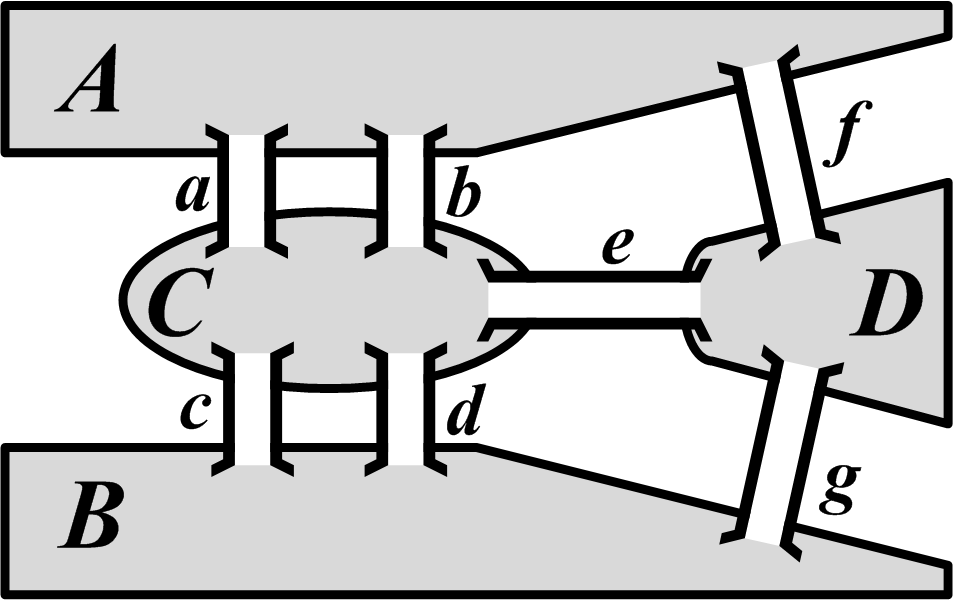
\includegraphics[width=0.3\textwidth]{fig/kenigsberg.png}
        }
        &
        \(
            {\xymatrix{
                A \ar@{-}@/^/[d]^b \ar@{-}@/_/[d]_a \ar@{-}@/^/[dr]^f
                    &*{}
                        \\
                C \ar@{-}[r]^e
                    &D
                        \\
                B \ar@{-}@/^/[u]^c \ar@{-}@/_/[u]_d \ar@{-}@/_/[ur]_g
                    &*{}
            }}
        \)        
    \end{tabular}
    \caption{Задача о Кенигсбергских мостах}
    \label{fig:graph:kenigsberg}
\end{figure}


Ныне теория графов --- это один из важнейших разделов дискретной математики, находящий массу практических применений в первую очередь из за своей наглядности. Графами моделируются схемы дорог, электрические схемы, химические соединения, схемы управления, автоматы, отношения и т.д. Для углубленного изучения теории графов можно рекомендовать книги: \cite{bib:shaporev:discretemath, bib:gorbatovs:discrmath, bib:novic:discrmathprogrammer}. Свободное изложение основ теории графов можно найти в книге \cite{bib:ore:graphs}.


\section{Основные термины и определения}

Граф $G$ --- это совокупность $G=\langle V,P\rangle$ \emph{множества} вершин $V$ и \emph{набора} отрезков $P$, соединяющих пары вершин. Отдельный отрезок представлен упорядоченной $(a,b)$ (или неупорядоченной $[a,b]$) парой, где $a,b\in V$. В общем случае, в наборе $P$ могут присутствовать несколько одинакового вида пар $(a,b)$.

Отрезок $[a,a]$, соединяющий вершину $a$ с ней самой, называется \emph{петлей}.

Неупорядоченная пара вершин $[a,b]$ (т.е. $[a,b]=[b,a]$) называется \emph{ребром}, а граф, содержащий только ребра называется \emph{неориентированным}.

Упорядоченная пара вершин $(a,b)$ (т.е. $(a,b)\neq(b,a)$) называется \emph{дугой}, а граф, содержащий только дуги называется \emph{ориентированным} или \emph{орграфом}. Дуга изображается стрелкой.

Если набор $P$ содержит несколько одинаковых отрезков-пар, то такие пары называются \emph{кратными}, а граф называется \emph{мультиграфом}.

Если задана функция $f:V\to M$ и/или $f:P\to M$, то множество $M$ называтется множеством \emph{пометок}, а граф называется \emph{помеченным}\footnote{Граф на рисунке \ref{fig:graph:kenigsberg} --- помеченный} (или \emph{нагруженным}). Пометка на изображении графа пишется над соответствующей вершиной или отрезком. Если пометка представляет собой число (или элемент упорядоченного множества), то она называется \emph{весом}, а граф --- \emph{взвешенным}.

Вершины, соединенные одним ребром, называются \emph{смежными}. Ребра, имеющие общую вершину, также называются \emph{смежными}. Ребро \emph{инцидентно} вершинам, которые оно соединяет, и вершины также \emph{инцидентны} этому ребру.

\emph{Степенью} вершины называется число ребер, инцидентных этой вершине. В орграфах различают полустепени исхода (количество исходящих дуг) и захода (количество входящих дуг).

Граф называется \emph{полным}, если между любыми его вершинами существует ребро. В полном графе с $n$ вершинами число ребер $m=\frac{n(n-1)}{2}$. \emph{Дополнение} графа до полного содержит все ребра полного графа, не принадлежащие исходному графу.

\emph{Подграфом} называется граф, в который входит лишь часть вершин исходного графа и часть его ребер, эти вершины соединяющих.

Последовательность 
\begin{equation}
    \label{eq:graph:path}
    v_1,p_1,v_2,p_2,\ldots,p_{n},v_{n+1},
\end{equation}
где $v_1,v_2,\ldots,v_{n+1}\in V$, $p_1,p_2,\ldots,p_{n}\in P$ и любые два соседних элемента инцидентны (т.е. $p_i=(v_i,v_{i+1}), 1\leq i\leq n$) называется \emph{$(v_1,v_{n+1})$-маршрутом}. $n$ --- число отрезков $p_i$ маршрута называется его \emph{длиной}.

Если все отрезки маршрута (кроме, возможно $p_1$ и $p_{n-1}$) различны, то он называется \emph{цепью}. Если все вершины маршрута (кроме, возможно $v_1$ и $v_{n+1}$) различны (а значит и отрезки), то маршрут называется \emph{простой} цепью.

Замкнутая ($v_1=v_n$) цепь называется \emph{циклом}. Замкнутая простая цепь называется \emph{простым} циклом.

В орграфе цепь называется \emph{путем}, а цикл --- \emph{контуром}.


\section{Способы задания графов}

Существует множество способов задать граф (см. рис. \ref{fig:graph:representation}):
\begin{itemize}
    \item аналитически;
    \item матрицей инцидентности;
    \item матрицей смежности;
    \item списком смежности.
\end{itemize}

\begin{figure}
    \centering

    \begin{tabular}{|c|c|c|}
        \hline
        &&\\
        {\xymatrix{
            a \ar@{->}[r]^2
                &b
                    \\
            c \ar@{->}[r]_5 \ar@{->}[ur]^3 \ar@{->}[u]^1
                &d \ar@{->}[u]_4
        }}
        &
        \raisebox{-.5\height}{
            \(
                \begin{array}{c|cccc}
                     &a&b&c&d\\\hline
                    a&0&1&0&0\\
                    b&0&0&0&0\\
                    c&1&1&0&1\\
                    d&0&1&0&0
                \end{array}
            \)
        }
        &
        \raisebox{-.5\height}{
            \(
                \begin{array}{c|ccccc}
                      & 1 & 2& 3& 4& 5\\ \hline 
                    a & -1& 1& 0& 0& 0\\
                    b & 0 &-1&-1&-1& 0\\
                    c & 1 & 0& 1& 0& 1\\
                    d & 0 & 0& 0& 1&-1
                \end{array}
            \)
        }
        \\ \cline{2-3}
        &\multicolumn{2}{|c|}{
        \(
            \{a\mapsto\{b\},b\mapsto\emptyset,
            c\mapsto\{a,b,d\},d\mapsto\{b\}\}
        \)
        }
        \\ \hline
    \end{tabular}
    \caption{Способы задания графов}
    \label{fig:graph:representation}
\end{figure}

Граф $G=\langle V,P\rangle$ можно задать аналитически, перечислив множество вершин $V$ и набор отрезков $P$.

Пусть $n=|V|$ --- количество вершин, а $m=|P|$ --- количество отрезков. 

Элементы \emph{матрицы инцидентности} $[G]_{n\times m}$ неориентированного графа определяются так:
\[
    [G]_{i,j}=
    \begin{cases}
        1, &\text{если вершина $v_i\in V$ инцидентна ребру $p_j\in P$},\\
        0, &\text{в противном случае.}
    \end{cases}
\]

В каждом $j$-м столбце матрицы по две $1$, если $p_j$ не петля, и одна в противном случае. 

Для орграфа элементы \emph{матрицы инцидентности} $[G]_{n\times m}$ определяются так:
\[
    [G]_{i,j}=
    \begin{cases}
         1, &\text{если вершина $v_i\in V$ --- начало дуги $p_j\in P$},\\
        -1, &\text{если вершина $v_i\in V$ --- конец дуги $p_j\in P$},\\
         0, &\text{в противном случае.}
    \end{cases}
\]

\emph{Матрица смежности вершин} $[G]_{n\times n}$:
\[
    [G]_{i,j}=
    \begin{cases}
         1, &\text{если $(v_i,v_j)\in P$},\\
         0, &\text{в противном случае.}
    \end{cases}
\]

Для мультиграфа вместо $1$ указывается количество кратных отрезков $(v_i,v_j)$.

Для представления графов в компьютерах наиболее часто используется \emph{список смежности вершин} 
\[
    \{v\mapsto \{v_s|v_s\in V,(v,v_s)\in P\}|v\in V\},
\]
для каждой вершины $v$ определяющий множество смежных с ней вершин $v_s$.

Не следует забывать, что орграф задает бинарное отношение, а потому часть способов задания графа уже была рассмотрена в главе \ref{ch:rel:rel}.


\section{Связность}

\emph{Связным} называется граф, в котором любые две вершины соединены цепью. Максимальный по количеству вершин связный подграф графа называется его \emph{компонентой связности}. Граф называется \emph{несвязным}, если число его компонент связности больше одной. 

Для ориентированного графа вводится понятие \emph{сильной} связности: в таком орграфе любые две вершины соединены двумя путями: путем с началом в первой вершине, и путем с началом во второй.

\emph{Число вершинной связности} графа --- это наименьшее число вершин, удаление которых в связном графе приводит несвязному графу. \emph{Число реберной связности} графа --- это наименьшее число ребер, удаление которых в связном графе приводит несвязному графу.

\begin{exampl}
    \label{ex:graph:net}
    Рассмотрим сеть передачи данных, состоящую из узлов (компьютеров) и каналов передачи информации между ними. Эту сеть легко представить графом, вершины которого соответствуют узлам, а ребра --- каналам передачи информации. Сеть исправна, если любая пара узлов способна обмениваться информацией. Надежность (живучесть) сети --- способность функционировать при выходе из строя одного или нескольких узлов и(или) каналов. Допустим, имеется сеть следующей структуры:
    \[
        {\xymatrix{
            n_1 \ar@{-}[dd]_{c_{1,2}} \ar@{-}[dr]^{c_{1,3}}
                &*{}
                    &n_5 \ar@{-}[d]_{c_{5,6}} \ar@{-}[r]^{c_{5,8}}
                        &n_8
                            \\
            *{}
                &n_3 \ar@{-}[d]^{c_{3,4}} \ar@{-}[r]^{c_{3,6}}
                    &n_6 \ar@{-}[ur]_{c_{6,8}} \ar@{-}[dr]^{c_{6,9}} \ar@{-}[d]_{c_{6,7}}
                        &*{}
                            \\
            n_2 \ar@{-}[r]_{c_{2,4}}
                &n_4
                    &n_7 \ar@{-}[r]_{c_{7,9}}
                        &n_9
                            \\
        }}
    \]
    где $n_i$ --- $i$-й узел, а $c_{i,j}$ --- канал, соединяющий $i$-й и $j$-й узлы.
    
    Если выйдет из строя канал $c_{1,2}$, то узлы $n_1$ и $n_2$ не смогут обмениваться информацией непосредственно, но они могут передавать информацию маршрутом: 
    \[c_{1,3},n_3,c_{3,4},n_4,c_{2,4},n_2.\]
    
    Если из строя выйдет узел $n_1$, то это не лишит остальные узлы возможности обмена информацией. А вот выход из строя канала $c_{3,6}$ будет иметь плачевные последствия. Еще больший ущерб сети нанесет выход из строя узла $n_6$.
    
    Очевидно, что числа вершинной и реберной связности данного графа совпадают и равны $1$. Эти числа отражают устойчивость графа к разрушению.
    \qed
\end{exampl}

Ребро графа называется \emph{мостом}, если удаление его увеличивает число компонент связности графа. Вершина графа называется \emph{точкой сочленения} (разделяющей вершиной), если её удаление увеличивает число компонент связности графа. Граф, не имеющий точек сочленения, называется \emph{неразделимым}. \emph{Блок} графа --- максимальный незазделимый подграф. Для графа из примера \ref{ex:graph:net}:
\begin{itemize}
    \item мост --- $c_{3,6}$;
    \item точки сочленения --- $n_3,n_6$;
    \item блок --- $G'=\langle\{n_1,n_2,n_3,n_4\},\{c_{1,2},c_{1,3},c_{3,4},c_{2,4}\}\rangle$.
\end{itemize}

Для определения связности графа и выделения компонент связности вводятся понятия \emph{достижимости}, \emph{контрдостижимости} и \emph{взаимодостижимости} вершин. В орграфе вершина $v_j$ считается \emph{достижимой} из вершины $v_i$, если существует путь $(v_i,v_j)$; вершина $v_j$ считается \emph{контрдостижимой} из вершины $v_i$, если существует путь $(v_j,v_i)$. Вершины $v_i,v_j$ \emph{взаимодостижимы}, если $v_j$ одновременно достижима и контрдостижима из $v_i$.

Элемент матрицы достижимости $[R]$ определяется по правилу 
\[
    [R]_{i,j}=
    \begin{cases}
        1,&\text{если $v_j$ достижима из $v_i$},\\
        0,&\text{в противном случае}.
    \end{cases}
\]

Для матрицы контрдостижимости $[Q]$ характерно $[Q]=[R]^T$. Очевидно, что матрица достижимости соответствует транзитивному замыканию исходного отношения (заданного исходным графом см. главу \ref{ch:bo}). На основе матрицы смежности графа её можно получить, используя, например, алгоритм Уоршалла (см. псевдокод \ref{alg:bo:warshall}).

Можно использовать также следующий алгоритм получения матрицы достижимости.
\paragraph{Поиск матрицы достижимости по матрице смежности}
\begin{enumerate}
    \item Из матрицы смежности $[S]$ выписать единицы в формируемую строку матрицы достижимости $[R]$.
    \item Пусть $[R]_{l,k}=1$: в $l$-ю строку матрицы достижимости выписать $1$-цы из $k$-й строки матрицы смежности. Эту операцию выполнить для всех ненулевых элементов формируемой строки матрицы достижимости.
    \item После формирования всех строк матрицы достижимости на главной диагонали проставить $1$.
\end{enumerate}

Для неориентированных графов матрицы достижимости и взаимодостижимости совпадают, а для орграфов элементы матрицы взаимодостижимости $[H]$ находятся по правилу
\[
    [H]_{i,j}=
    \begin{cases}
        1,&\text{если $([R]_{i,j}=1)\land([R]_{j,i}=1)$},\\
        0,&\text{в противном случае}.
    \end{cases}
\]

Видно, что матрица $H$ задает транзитивное, рефлексивное и симметричное отношение, то есть отношение эквивалентности. Каждый класс эквивалентности данного отношения определяет множество взаимодостижимых вершин графа, то есть определяет вершины соответствующих компонент связности исходного графа.
\begin{exampl} 
    Задача. Дан орграф
    \[
        {\xymatrix{
            *{}
                &3 \ar@{->}@/^/[dl]
                    &5 \ar@{->}[l] \ar@{->}[d]
                        \\
            1 \ar@{->}@/^/[ur] \ar@{->}@/^/[d]
                &*{}
                    &6 \ar@{->}[d]
                        \\
            2 \ar@{->}@/^/[u] \ar@{->}[r]
                &4 \ar@{->}[ur]
                    &7 \ar@{->}[l]
        }}        
    \]
    
    Требуется выделить компоненты связности.
\end{exampl}
\begin{proof}[Решение]
    Матрица смежности для данного графа будет такой:
    \[
        [S]=
        \begin{array}{c|ccccccc}
             &1&2&3&4&5&6&7\\ \hline
            1&0&1&1&0&0&0&0\\
            2&1&0&0&1&0&0&0\\
            3&1&0&0&0&0&0&0\\
            4&0&0&0&0&0&1&0\\
            5&0&0&1&0&0&1&0\\
            6&0&0&0&0&0&0&1\\
            7&0&0&0&1&0&0&0
        \end{array}
    \]
    
    По матрице смежности находятся матрицы достижимости и взаимодостижимости:
    \[
        [R]=
        \begin{array}{c|ccccccc}
             &1&2&3&4&5&6&7\\ \hline
            1&1&1&1&1&0&1&1\\
            2&1&1&1&1&0&1&1\\
            3&1&1&1&1&0&1&1\\
            4&0&0&0&1&0&1&1\\
            5&1&1&1&1&1&1&1\\
            6&0&0&0&1&0&1&1\\
            7&0&0&0&1&0&1&1
        \end{array},
        [H]=
        \begin{array}{c|ccccccc}
                 &1&2&3&\fbox{5}
                         &4&6&7\\ \hline
                1&1&1&1&0&0&0&0\\
                2&1&1&1&0&0&0&0\\
                3&1&1&1&0&0&0&0\\
         \fbox{5}&0&0&0&1&0&0&0\\
                4&0&0&0&0&1&1&1\\
                6&0&0&0&0&1&1&1\\
                7&0&0&0&0&1&1&1
        \end{array}.
    \]
    
    Выделяются три класса эквивалентности:
    \[
        \{1,2,3\},\{5\},\{4,6,7\}.
    \]
    Которым соответствуют следующие компоненты сильной связности орграфа.
    \[
        {\xymatrix{
            *{}
                &3 \ar@{->}@/^/[dl]
                    &5 
                        \\
            1 \ar@{->}@/^/[ur] \ar@{->}@/^/[d]
                &*{}
                    &6 \ar@{->}[d]
                        \\
            2 \ar@{->}@/^/[u]
                &4 \ar@{->}[ur]
                    &7 \ar@{->}[l]
        }}        
    \]
\end{proof}

На практике чаще всего имеют дело с графами, имеющими только одну компоненту связности.


\section{Нахождение кратчайших маршрутов}

Пусть $G=\langle V,P\rangle,w:P\to\mathbb{R}$ --- взвешенный по отрезкам граф, имеющий $n$ вершин. Вес маршрута 
\[
    v_1,p_1,v_2,p_2,\ldots,p_{m},v_{m+1}
\]    
обычно находится так.
\begin{itemize}
    \item Сумма весов: $\displaystyle d(v_1,v_{m+1})=\sum_{i=1}^{m}w(p_i)$.
    
    \item Произведение весов $\displaystyle d(v_1,v_{m+1})=\prod_{i=1}^{m}w(p_i)$.
    В этом случае задачу сводят к сумме логарифмов весов:
    \[
        d'(v_1,v_{m+1})=\ln(d(v_1,v_{m+1}))=\sum_{i=1}^{m}\ln(w(p_i)).
    \]
\end{itemize}

Далее будем предполагать, что вес маршрута находится как сумма весов.

Орграф не должен содержать контуров, дуги которых имеют отрицательный вес (иначе возможно такое, что двигаясь по циклу некоторое число раз, можно получить вес меньше любого заданного числа, что сделает задачу бессмысленной).

Необходимо найти маршруты минимального веса из вершины $v_i\in V$ до всех остальных вершин графа. К решению данной задачи сводится множество практических задач: планировании поставок на транспорте, маршрутизации пакетов в компьютерных сетиях и т.д.

\paragraph{Алгоритм \emph{Форда-Беллмана}} выполняется следующим образом.
\begin{enumerate}
    \item Задается кортеж $D^{(1)}=(d_1^{(1)},d_2^{(1)},\ldots,d_n^{(1)})$, где $n=|V|$ --- количество вершин графа. $d_i^{(1)}=0$, а $d_j^{(1)}=w_{ij}, i\neq j$, где $w_{ij}$ --- вес отрезка $(v_i,v_j)$. Причем, если отрезка $(v_i,v_j)$ не существует в графе, то $w_{ij}=\infty$. Также $w_{ii}=0$. Устанавливается шаг: $s=1$.
    
    \item\label{en:graph:fordMain} На шаге $s$ определяется кортеж $D^{(s+1)}=(d_1^{(s+1)},d_2^{(s+1)},\ldots,d_n^{(s+1)})$. 
    \[
        d_j^{(s+1)}=\min[\{d_j^{(s)}\}\cup\{d_k^{(s)}+w_{kj}|1\leq k\leq n\}].
    \]
    
    \item $s\gets s+1$. Если $s=n-1$, то получен кортеж минимальных расстояний $D^{(s)}$ от вершины $v_i$ до всех остальных через маршруты, содержащие не более $n-1$ дуг. В этом случае алгоритм завершается, иначе происходит переход к шагу \ref{en:graph:fordMain}.
\end{enumerate}

Элементы $w_{i,j}$ удобно рассматривать в виде матрицы $[W]_{n\times n}$.
\begin{exampl}
    Пусть задан граф 
    \[    
        {\xymatrix{
            *{}
                &2 \ar@{->}[r]^3 \ar@{->}[ddr]_(.25){4}
                    &3
                        \\
            1 \ar@{->}[ur]^1 \ar@{->}[dr]_1
                &*{}
                    &*{}
                        \\
            *{}
                &4 \ar@{->}[uur]^(.25){2}
                    &5 \ar@{->}[l]^{-7} \ar@{->}[uu]_{1}
        }}
    \]    
    
    Необходимо найти веса кратчайших маршрутов из вершины $1$.
\end{exampl}
\begin{proof}[Решение]
    Графу будет соответствовать матрица $W$ весов $w_{ij}$
    \[
        W =
        \begin{array}{c|cccccc}
                &1      &2      &3      &4      &5      \\ \hline
            1   &0      &1      &\infty &1      &\infty \\
            2   &\infty &0      &3      &\infty &4      \\
            3   &\infty &\infty &0      &\infty &\infty \\
            4   &\infty &\infty &2      &0      &\infty \\
            5   &\infty &\infty &1      &-7     &0      \\
        \end{array}
    \]
    Выполним $4$ расчета $D^{(i)}$:
    \begin{enumerate}
        \item $D^{(1)}=(0,1,\infty,1,\infty)$. 
        \[
            \begin{split}
                d_1^{(1)}=w_{1,1}=0,\\
                d_2^{(1)}=w_{1,2}=1,\\
                d_3^{(1)}=w_{1,3}=\infty,\\
                d_4^{(1)}=w_{1,4}=1,\\
                d_5^{(1)}=w_{1,5}=\infty.
            \end{split}
        \]
        
        \item $D^{(2)}=(0,1,3,1,5)$;
        \[
            \begin{split}
                d_1^{(2)}=\min[\{
                    d_1^{(1)},
                    d_1^{(1)}+w_{1,1},
                    d_2^{(1)}+w_{2,1},
                    d_3^{(1)}+w_{3,1},
                    d_4^{(1)}+w_{4,1},
                    d_5^{(1)}+w_{5,1}
                \}]=\\
                =\min[\{
                    0,0,\infty,\infty,\infty,\infty
                \}] = w_{1,1}=0,\\
                d_2^{(2)}=\min[\{
                    d_2^{(1)},
                    d_1^{(1)}+w_{1,2},
                    d_2^{(1)}+w_{2,2},
                    d_3^{(1)}+w_{3,2},
                    d_4^{(1)}+w_{4,2},
                    d_5^{(1)}+w_{5,2}
                \}]=\\
                =\min[\{
                    1,1,\infty,\infty,\infty,\infty
                \}] = w_{1,2}=1,\\
                d_3^{(2)}=\min[\{
                    d_3^{(1)},
                    d_1^{(1)}+w_{1,3},
                    d_2^{(1)}+w_{2,3},
                    d_3^{(1)}+w_{3,3},
                    d_4^{(1)}+w_{4,3},
                    d_5^{(1)}+w_{5,3}
                \}]=\\
                =\min[\{
                    \infty,\infty,4,\infty,3,\infty
                \}] = w_{1,4}+w_{4,3}=3,\\
                d_4^{(2)}=\min[\{
                    d_4^{(1)},
                    d_1^{(1)}+w_{1,4},
                    d_2^{(1)}+w_{2,4},
                    d_3^{(1)}+w_{3,4},
                    d_4^{(1)}+w_{4,4},
                    d_5^{(1)}+w_{5,4}
                \}]=\\
                =\min[\{
                    1,1,\infty,\infty,1,\infty
                \}] = w_{1,4}=1,\\
                d_5^{(2)}=\min[\{
                    d_5^{(1)},
                    d_1^{(1)}+w_{1,5},
                    d_2^{(1)}+w_{2,5},
                    d_3^{(1)}+w_{3,5},
                    d_4^{(1)}+w_{4,5},
                    d_5^{(1)}+w_{5,5}
                \}]=\\
                =\min[\{
                    \infty,\infty,5,\infty,\infty,\infty
                \}] = w_{1,2}+w_{2,5}=5.
            \end{split}
        \]
        
        \item $D^{(3)}=(0,1,3,-2,5)$. 
        \[
            \begin{split}
                d_1^{(3)}=d_1^{(2)}=w_{1,1}=0,\\
                d_2^{(3)}=d_2^{(2)}=w_{1,2}=1,\\
                d_3^{(3)}=d_4^{(2)}+w_{4,3}=w_{1,4}+w_{4,3}=3,\\
                d_4^{(3)}=d_5^{(2)}+w_{5,4}=w_{1,2}+w_{2,5}+w_{5,4}=-2,\\
                d_5^{(3)}=d_5^{(2)}=w_{1,2}+w_{2,5}=5.
            \end{split}
        \]
        
        \item $D^{(4)}=(0,1,0,-2,5)$. 
        \[
            \begin{split}
                d_1^{(4)}=d_1^{(3)}=w_{1,1}=0,\\
                d_2^{(4)}=d_2^{(3)}=w_{1,2}=1,\\
                d_3^{(4)}=d_4^{(3)}+w_{4,3}=w_{1,2}+w_{2,5}+w_{5,4}+w_{4,3}=0,\\
                d_4^{(4)}=d_4^{(3)}=w_{1,2}+w_{2,5}+w_{5,4}=-2,\\
                d_5^{(4)}=d_5^{(3)}=w_{1,2}+w_{2,5}=5.
            \end{split}
        \]        
    \end{enumerate}
    
    Кроме весов кратчайших маршрутов получены также и сами маршруты, которые легко определяются по входящим в итоговую сумму $w_{ij}$. 
    \[    
        {\xymatrix{
            *{}
                &2 \ar@{->}[r]^3 \ar@{:>}[ddr]_(.25){4}
                    &3
                        \\
            1 \ar@{:>}[ur]^1 \ar@{->}[dr]_1
                &*{}
                    &*{}
                        \\
            *{}
                &4 \ar@{:>}[uur]^(.25){2}
                    &5 \ar@{:>}[l]^{-7} \ar@{->}[uu]_{1}
        }}
    \]        
    Например, кратчайший $(1,3)$-маршрут\footnote{Из представления маршрута (формула \eqref{eq:graph:path}) исключены отрезки $p_i$, потому что каждую пару вершин соединяет только одна дуга соответствующего направления}: $1,2,5,4,3$.
\end{proof}

Если веса дуг неотрицательны, можно использовать более производительный алгоритм Дейкстры. Задача остается прежней: необходимо найти маршруты минимального веса из вершины $v_i\in V$ до всех остальных вершин графа.
\paragraph{Алгоритм \emph{Дейкстры}} выполняется следующим образом.
\begin{enumerate}
    \item Задается кортеж $D^{(1)}=(d_1^{(1)},d_2^{(1)},\ldots,d_n^{(1)})$, где $n=|V|$ --- количество вершин графа. $d_i^{(1)}=0$, а $d_j^{(1)}=w_{ij}, i\neq j$, где $w_{ij}$ --- вес отрезка $(v_i,v_j)$. Причем, если отрезка $(v_i,v_j)$ не существует в графе, то $w_{ij}=\infty$. Также $w_{ii}=0$. Кроме того, вводится множество $T^{(1)}$ вершин, кратчайший маршрут к которым еще не проложен: $T^{(1)}=V\backslash\{v_i\}$. Устанавливается шаг: $s=1$.
    
    \item\label{en:graph:dejkstraMain} На шаге $s$ среди вершин, маршрут к которым еще не проложен, выбирается вершина $v_k\in T^{(s)}$, маршрут до которой является кратчайшим: $d_k^{(s)}=\min\{d_j^{(s)}|v_j\in T^{(s)}\}$.
    
    Выбранная вершина $v_k$ исключается из дальнейшего рассмотрения $T^{(s+1)}=T^{(s)}\backslash\{v_k\}$.
    Определяется строка $D^{(s+1)}=(d_1^{(s+1)},d_2^{(s+1)},\ldots,d_n^{(s+1)})$. Причем, если $v_j\in T^{(s+1)}$, то 
    \[
        d_j^{(s+1)}=\min\{d_j^{(s)}, d_k^{(s)}+w_{kj}\},
    \]
    а если $v_j\not\in T^{(s+1)}$, то $d_j^{(s+1)}=d_j^{(s)}$.
    
    \item $s\gets s+1$. Если $s=n-1$, то получены минимальные расстояния $D^{(s)}$ от вершины $v_i$ до всех остальных через маршруты, содержащие не более $n-1$ дуг, и в этом случае алгоритм завершается, иначе происходит переход к шагу \ref{en:graph:dejkstraMain}.
\end{enumerate}

\begin{exampl}
    Пусть задан граф 
    \[    
        {\xymatrix{
            *{}
                &2 \ar@{->}[rr]^1 \ar@{->}@/^/[dd]^(.4)2 \ar@{->}@/^/[dl]^(.75)1
                    &*{}
                        &5 \ar@{->}@/^/[dl]^(.6)2
                            \\
            1 \ar@{->}@/^/[ur]^3 \ar@{->}[dr]_7
                &*{}
                    &4 \ar@{->}@/^/[ur]^(.4)5 \ar@{->}[dr]^1
                        &*{}
                            \\
            *{}
                &3 \ar@{->}@/^/[uu]^(.4)1 \ar@{->}[ur]^(.65)4 \ar@{->}@/^/[rr]^4
                    &*{}
                        &6 \ar@{->}@/^/[ll]^1 \ar@{->}[uu]_3
        }}
    \]    
    
    Необходимо найти веса кратчайших маршрутов из вершины $1$.
\end{exampl}
\begin{proof}[Решение]
    Графу будет соответствовать матрица $W$ весов $w_{ij}$
    \[
        W =
        \begin{array}{c|cccccc}
                &1      &2      &3      &4      &5      &6      \\ \hline
            1   &0      &3      &7      &\infty &\infty &\infty \\
            2   &1      &0      &2      &\infty &1      &\infty \\
            3   &\infty &1      &0      &4      &\infty &4      \\
            4   &\infty &\infty &\infty &0      &5      &1      \\
            5   &\infty &\infty &\infty &2      &0      &\infty \\
            6   &\infty &\infty &1      &\infty &3      &0
        \end{array}
    \]
    Выполним $5$ расчетов $D^{(i)}$:
    \begin{enumerate}
        \item $D^{(1)}=(\fbox{0},3,7,\infty,\infty,\infty)$, $T^{(1)}=\{2,3,4,5,6\}$. 
        \[
            \begin{split}
                d_1^{(1)}=w_{1,1}=0,\\
                d_2^{(1)}=w_{1,2}=3,\\
                d_3^{(1)}=w_{1,3}=7,\\
                d_4^{(1)}=w_{1,4}=\infty,\\
                d_5^{(1)}=w_{1,5}=\infty,\\
                d_5^{(1)}=w_{1,5}=\infty.
            \end{split}
        \]
        
        \item т.к. $d_2^{(1)}=\min\{d_2^{(1)},d_3^{(1)},d_4^{(1)},d_5^{(1)},d_6^{(1)}\}=3$, то $T^{(2)}=\{3,4,5,6\}$.
        \[
            \begin{split}
                d_1^{(2)}=d_1^{(1)}=w_{1,1}=0,\\
                d_2^{(2)}=d_2^{(1)}=w_{1,2}=3,\\
                d_3^{(2)}=\min\{d_3^{(1)}, d_2^{(1)}+w_{2,3}\}=d_2^{(1)}+w_{2,3}=w_{1,2}+w_{2,3}=5,\\
                d_4^{(2)}=\min\{d_4^{(1)}, d_2^{(1)}+w_{2,4}\}=\infty,\\
                d_5^{(2)}=\min\{d_5^{(1)}, d_2^{(1)}+w_{2,5}\}=d_2^{(1)}+w_{2,5}=w_{1,2}+w_{2,5}=4,\\
                d_6^{(2)}=\min\{d_6^{(1)}, d_2^{(1)}+w_{2,6}\}=\infty.\\
            \end{split}
        \]
        
        Тогда 
        \[
            D^{(2)}=(\fbox{0},\fbox{3},5,\infty,4,\infty).
        \]
        
        \item т.к. $d_5^{(2)}=\min\{d_3^{(2)},d_4^{(2)},d_5^{(2)},d_6^{(2)}\}=4$, то $T^{(3)}=\{3,4,6\}$.
        \[
            \begin{split}
                d_1^{(3)}=d_1^{(2)}=w_{1,1}=0,\\
                d_2^{(3)}=d_2^{(2)}=w_{1,2}=3,\\
                d_3^{(3)}=\min\{d_3^{(2)}, d_5^{(2)}+w_{5,3}\}=d_3^{(2)}=w_{1,2}+w_{2,3}=5,\\
                d_4^{(3)}=\min\{d_4^{(2)}, d_5^{(2)}+w_{5,4}\}=d_5^{(2)}+w_{5,4}=w_{1,2}+w_{2,5}+w_{5,4}=6,\\
                d_5^{(3)}=d_5^{(2)}=w_{1,2}+w_{2,5}=4,\\
                d_6^{(3)}=\min\{d_6^{(2)}, d_5^{(2)}+w_{5,6}\}=\infty.\\
            \end{split}
        \]
        
        Тогда
        \[
            D^{(3)}=(\fbox{0},\fbox{3},5,6,\fbox{4},\infty).
        \]

        \item т.к. $d_3^{(3)}=\min\{d_3^{(3)},d_4^{(3)},d_6^{(3)}\}=5$, то $T^{(4)}=\{4,6\}$.
        \[
            \begin{split}
                d_1^{(4)}=d_1^{(3)}=w_{1,1}=0,\\
                d_2^{(4)}=d_2^{(3)}=w_{1,2}=3,\\
                d_3^{(4)}=d_3^{(3)}=w_{1,2}+w_{2,3}=5,\\
                d_4^{(4)}=\min\{d_4^{(3)}, d_3^{(3)}+w_{3,4}\}=d_4^{(3)}=w_{1,2}+w_{2,5}+w_{5,4}=6,\\
                d_5^{(4)}=d_5^{(3)}=w_{1,2}+w_{2,5}=4,\\
                d_6^{(4)}=\min\{d_6^{(3)}, d_3^{(3)}+w_{3,6}\}=d_3^{(3)}+w_{3,6}=w_{1,2}+w_{2,3}+w_{3,6}=9.\\
            \end{split}
        \]
        
        Тогда
        \[
            D^{(4)}=(\fbox{0},\fbox{3},\fbox{5},6,\fbox{4},9).
        \]

        \item т.к. $d_4^{(4)}=\min\{d_4^{(4)},d_6^{(4)}\}=6$, то $T^{(5)}=\{6\}$.
        \[
            \begin{split}
                d_1^{(5)}=d_1^{(4)}=w_{1,1}=0,\\
                d_2^{(5)}=d_2^{(4)}=w_{1,2}=3,\\
                d_3^{(5)}=d_3^{(4)}=w_{1,2}+w_{2,3}=5,\\
                d_4^{(5)}=d_4^{(4)}=w_{1,2}+w_{2,5}+w_{5,4}=6,\\
                d_5^{(5)}=d_5^{(4)}=w_{1,2}+w_{2,5}=4,\\
                d_6^{(5)}=\min\{d_6^{(4)}, d_4^{(4)}+w_{4,6}\}=w_{1,2}+w_{2,5}+w_{5,4}+w_{4,6}=7.\\
            \end{split}
        \]
        
        Тогда
        \[
            D^{(5)}=(\fbox{0},\fbox{3},\fbox{5},\fbox{6},\fbox{4},7).
        \]        
    \end{enumerate}
    
    Кроме кортежа весов кратчайших маршрутов $D^{(5)}$ получены также и сами маршруты, которые легко определяются по входящим в итоговую сумму $w_{ij}$. 
    \[    
        {\xymatrix{
            *{}
                &2 \ar@{:>}[rr]^1 \ar@{:>}@/^/[dd]^(.4)2 \ar@{->}@/^/[dl]^(.75)1
                    &*{}
                        &5 \ar@{:>}@/^/[dl]^(.6)2
                            \\
            1 \ar@{:>}@/^/[ur]^3 \ar@{->}[dr]_7
                &*{}
                    &4 \ar@{->}@/^/[ur]^(.4)5 \ar@{:>}[dr]^1
                        &*{}
                            \\
            *{}
                &3 \ar@{->}@/^/[uu]^(.4)1 \ar@{->}[ur]^(.65)4 \ar@{->}@/^/[rr]^4
                    &*{}
                        &6 \ar@{->}@/^/[ll]^1 \ar@{->}[uu]_3
        }}
    \]    
    
    Например, кратчайший $(1,4)$-маршрут: $1,2,5,4$.
\end{proof}


\section{Деревья}

\emph{Деревом} называется:
\begin{itemize}
    \item произвольный связный неориентированный граф без циклов;
    \item связный граф без циклов, содержащий $n$ вершин и $n-1$ ребро;
    \item граф в котором каждая пара вершин соединена одной и только одной простой цепью.
\end{itemize}

Для любого связного графа с $n$ вершинами можно построить дерево с таким же количеством вершин. Такое дерево называется \emph{покрывающим} деревом, \emph{каркасом} или \emph{остовом}.


\paragraph{Алгоритм выделения каркаса связного графа $G=\langle V,P\rangle,|V|=n$}
\begin{enumerate}
    \item Произвольно выбирается $v_i\in V$. Подграф $G_1=\langle \{v_i\},\emptyset\rangle$ --- дерево. Устанавливается шаг: $s=1$.
    
    \item\label{en:graph:sceletonMain} Если $s=n$, то задача решена, алгоритм завершается.
    
    \item На шаге $s$ уже построено дерево $G_s=\langle V_s,P_s\rangle$. Произвольно выбирается вершина $v_i$ не входящая в $G_s$: $(v_i\in V)\land (v_i\not\in V_s)$, смежная с некоторой вершиной\footnote{Такая, в силу связности графа, обязательно найдется} $v_j\in V_s$: $([v_i,v_j]\in P)\land(v_j\in V_s)$. Образуется новый граф $G_{s+1}=\langle V_s\cup\{v_i\},P_s\cup\{[v_i,v_j]\}\rangle$, который также является деревом. $s\gets s+1$. Переход к шагу \ref{en:graph:sceletonMain}.
\end{enumerate}

Следствием из данного алгоритма является соотношение $m=n-1$, где $m$ --- количество рёбер каркаса, а $n$ --- количество вершин исходного графа.

Видно, что вариантов выбора получается много. Так для полного графа с $n$ вершинами, количество возможных остовов составляет $n^{n-2}$.

Больший интерес представляет поиск остова минимального веса во взвешенном по дугам графе. Эту задачу решает алгоритм Краскала.
\paragraph{Алгоритм Краскала. $G=\langle V,P\rangle,w:P\to\mathbb{R},|V|=n$}
\begin{enumerate}
    \item Выбирается ребро $[v_i,v_j]\in P$ минимального веса. Подграф 
    \[
        G_1=\langle \{v_i, v_j\}, \{[v_i, v_j]\}\rangle
    \] 
    --- дерево. Устанавливается шаг: $s=1$.
    
    \item\label{en:graph:kraskalMain} Если $s=n-1$, то задача решена, алгоритм завершается.
    
    \item На шаге $s$ уже построен остов $G_s=\langle V_s,P_s\rangle$. Выбирается ребро минимального веса $[v_i,v_j]$, такое что $v_i\in V_s$, а $v_j\not\in V_s$. Образуется новый граф $G_{s+1}=\langle V_s\cup\{v_j\},P_s\cup\{[v_i,v_j]\}\rangle$, который также является деревом. $s\gets s+1$. Переход к шагу \ref{en:graph:kraskalMain}.
\end{enumerate}


\begin{exampl}
    Пусть задан граф 
    \[    
        {\xymatrix{
            *{}
                &{2} \ar@{-}[dd]^2 \ar@{-}[dr]^7
                    &*{}
                        &*{}
                            \\
            *{}
                &*{}
                    &{5} \ar@{-}[dr]^5 \ar@{-}[dd]^1
                        &*{}
                            \\
            {1} \ar@{-}[uur]^2 \ar@{-}[ddr]_4 \ar@{-}[r]^5
                &{3} \ar@{-}[dd]^1 \ar@{-}[ur]^4  \ar@{-}[dr]_3
                    &*{}
                        &{7}
                            \\
            *{}
                &*{}
                    &{6} \ar@{-}[ur]_7
                        &*{}
                            \\
            *{}
                &{4} \ar@{-}[ur]_4
                    &*{}
                        &*{}
        }}
    \]    
    
    Необходимо найти веса остов минимального веса.
\end{exampl}
\begin{proof}[Решение]
    Пройдем алгоритм по шагам. $n=7$.
    \begin{enumerate}
        \item $G_1=\langle\{3,4\},\{[3,4]\}\rangle$.
        \item $G_2=\langle\{2,3,4\},\{[3,4],[3,2]\}\rangle$.
        \item $G_3=\langle\{1,2,3,4\},\{[3,4],[3,2],[1,2]\}\rangle$.
        \item $G_4=\langle\{1,2,3,4,6\},\{[3,4],[3,2],[1,2],[3,6]\}\rangle$.
        \item $G_5=\langle\{1,2,3,4,5,6\},\{[3,4],[3,2],[1,2],[3,6],[6,5]\}\rangle$.
        \item $G_6=\langle\{1,2,3,4,5,6,7\},\{[3,4],[3,2],[1,2],[3,6],[6,5],[5,7]\}\rangle$.
    \end{enumerate}
    Получен остов
    \[    
        {\xymatrix{
            *{}
                &{2} \ar@{:}[dd]^2 \ar@{-}[dr]^7
                    &*{}
                        &*{}
                            \\
            *{}
                &*{}
                    &{5} \ar@{:}[dr]^5 \ar@{:}[dd]^1
                        &*{}
                            \\
            {1} \ar@{:}[uur]^2 \ar@{-}[ddr]_4 \ar@{-}[r]^5
                &{3} \ar@{:}[dd]^1 \ar@{-}[ur]^4  \ar@{:}[dr]_3
                    &*{}
                        &{7}
                            \\
            *{}
                &*{}
                    &{6} \ar@{-}[ur]_7
                        &*{}
                            \\
            *{}
                &{4} \ar@{-}[ur]_4
                    &*{}
                        &*{}
        }}
    \]    
    с весом $14$.
\end{proof}


\section{Изоморфизм}

Изоморфизм --- равенство форм. Один и тот же граф можно вычертить по-разному (см. рис. \ref{fig:graph:izomorpic}). Новый граф можно получить из некоторого графа просто переобозначив вершины. Все такие графы имеют одинаковую структуру.

\begin{figure}
    \[
        \begin{tabular}{cc}
            \(
                {\xymatrix{
                    1 \ar@{-}[d] \ar@{-}[dr] \ar@{-}[drr]
                        &2 \ar@{-}[dl] \ar@{-}[d] \ar@{-}[dr]
                            &3 \ar@{-}[dll] \ar@{-}[dl] \ar@{-}[d]
                                \\
                    4
                        &5
                            &6
                }}
            \)
                &
                \(
                    {\xymatrix{
                        1 \ar@{-}[d] \ar@{-}[r] \ar@{-}[drr]
                            &5 
                                &3 \ar@{-}[dll] \ar@{-}[l] \ar@{-}[d]
                                    \\
                        4
                            &2 \ar@{-}[l] \ar@{-}[u] \ar@{-}[r]
                                &6
                    }}
                \)
                    \\
                    &\\
            \(
                {\xymatrix{
                    1 \ar@{-}[d] \ar@{-}[r] \ar@{-}`u[r]`r[rr][rr]
                        &5 \ar@{-}[dr]\ar@{-}[d]
                            &6 \ar@{-}[d]
                                \\
                    4 \ar@{-}[r] \ar@{-}`d[rr]`[rr][rr]
                        &2 \ar@{-}[ur]
                            &3
                }}
            \)
                &
                \raisebox{-.5\height}{
                    \(
                        S=
                        \begin{array}{c|cccccc}
                             &1&2&3&4&5&6\\ \hline
                            1&0&0&0&1&1&1\\
                            2&0&0&0&1&1&1\\
                            3&0&0&0&1&1&1\\
                            4&1&1&1&0&0&0\\
                            5&1&1&1&0&0&0\\
                            6&1&1&1&0&0&0
                        \end{array}
                    \)        
                }
        \end{tabular}
    \]
    \caption{Изоморфные графы: $f=I_V$}
    \label{fig:graph:izomorpic}
\end{figure}

Два графа $G_1=\langle V_1,P_1\rangle$ и $G_2=\langle V_2,P_2\rangle$ называются \emph{изоморфными}, если существует биекция $f:V_1\leftrightarrow V_2$ такая, что $(v_i,v_j)\in P_1$ тогда и только тогда, когда $(f(v_i),f(v_j))\in P_2$. При этом функция $f$ называется \emph{изоморфизмом}.

Изоморфные графы образуют класс эквивалентности на множестве всех возможных графов. Графы имеют некоторые характеристики, совпадение которых свидительствует о возможности существования изоморфизма:
\begin{itemize}
    \item если у графа существует простой цикл, то в изоморфном графе также должен существовать простой цикл с таким же количеством вершин;
    \item если два простых цикла у графа имеют общие вешнины или рёбра, то в изоморфном графе существуют простые циклы с тем же количеством вершин и с тем же количеством общих вершин или рёбер\ldots
\end{itemize}

Графы $G_1,G_2$ на рисунке \ref{fig:graph:nonIzomorphic8} не изоморфны, потому что:
\begin{figure}
    \[
        \begin{tabular}{cc}
        {\xymatrix{
            1 \ar@{-}[rrr] \ar@{-}[ddd] \ar@{-}[dr]
                &*{}
                    &*{}
                        &2 \ar@{-}[ddd]
                            \\
            *{}
                &5 \ar@{-}[r] \ar@{-}[d]
                    &6 \ar@{-}[d]
                        &*{}
                            \\
            *{}
                &8 \ar@{-}[r]
                    &7
                        &*{}
                            \\
            4 \ar@{-}[ur]
                &*{}
                    &*{}
                        &3 \ar@{-}[lll]
        }}
        &
        {\xymatrix{
            a \ar@{-}[rrr] \ar@{-}[ddd] \ar@{-}[dr]
                &*{}
                    &*{}
                        &b \ar@{-}[ddd]
                            \\
            *{}
                &e \ar@{-}[r] \ar@{-}[d]
                    &f \ar@{-}[d]
                        &*{}
                            \\
            *{}
                &g \ar@{-}[r]
                    &h\ar@{-}[dr]
                        &*{}
                            \\
            d 
                &*{}
                    &*{}
                        &c \ar@{-}[lll]
        }}
        \\
        $G_1$&$G_2$
        \end{tabular}
    \]
    \caption{Не изоморфные графы}
    \label{fig:graph:nonIzomorphic8}
\end{figure}

\begin{itemize}
    \item в $G_1$ есть цикл из восьми ребер $1,2,3,4,8,7,6,5,1$, а в $G_2$ его нет;
    \item в $G_1$ ребро $[5,8]$ общее для двух циклов длины $4$, а в $G_2$ такого ребра нет нет\ldots
\end{itemize}

Числовая характеристика графа называются \emph{инвариантом}. Примерами инвариантов могут служить:
\begin{itemize}
    \item количество вершин;
    \item количество ребер;
    \item степени вершин\ldots
\end{itemize}

Но не существует ни одного инварианта однозначно определяющего наличие измомрфизма. Графы на рисунке \ref{fig:graph:nonIzomorphic6} не изоморфны (например, в $G_2$ есть два простых цикла длины $3$, а в $G_1$ таковых нет вообще), хотя все перечисленные выше инварианты совпадают.
\begin{figure}
    \[
        \begin{tabular}{cc}
        {\xymatrix{
            1 \ar@{-}[rrr] \ar@{-}[dd] \ar@{-}[dr]
                &*{}
                    &*{}
                        &2 \ar@{-}[dd] \ar@{-}[dl]
                            \\
            *{}
                &5 \ar@{-}[r] \ar@{-}[drr]
                    &6 \ar@{-}[dll]
                        &*{}
                            \\
            4 
                &*{}
                    &*{}
                        &3 \ar@{-}[lll]
        }}
        &
        {\xymatrix{
            a \ar@{-}[rrr] \ar@{-}[dd] \ar@{-}[dr]
                &*{}
                    &*{}
                        &b \ar@{-}[dd] \ar@{-}[dl]
                            \\
            *{}
                &e \ar@{-}[r] \ar@{-}[dl]
                    &f \ar@{-}[dr]
                        &*{}
                            \\
            d 
                &*{}
                    &*{}
                        &c \ar@{-}[lll]
        }}
        \\
        $G_1$&$G_2$
        \end{tabular}
    \]
    \caption{Не изоморфные графы (одинаковые инварианты)}
    \label{fig:graph:nonIzomorphic6}
\end{figure}

Процесс определения изоморфизма графов состоит в последовательном разбиении множества вершин каждого графа на подмножества вершин, имеющих одинаковую степень, с дальнейшим определением количества связей между выделенными подмножетвами. На каждом шаге вариантов разбиения может быть несколько. Задача поиска изоморфизма двух графов является вычислительно сложной\footnote{То есть для графов с очень большим количеством вершин она не решается на компьютере за приемлемое время}.

\begin{exampl} Найти изоморфизм графов, представленных на рисунке \ref{fig:graph:izomorphicAlgTask}.
    \begin{figure}
        \centering
        \begin{tabular}{cc}
            {\entrymodifiers={++[o][F-]}
                {\xymatrix@=.9pc{
                    1 \ar@{-}[d] \ar@{-}[dr] \ar@{-}[r]
                        &2 \ar@{-}[d] \ar@{-}[r]
                            &3 \ar@{-}[d] \ar@{-}[dl] \ar@{-}[dll]
                                \\
                    6
                        &5 \ar@{-}[l]
                            &4 \ar@{-}[l]
                }}
            }
            &
            {\entrymodifiers={++[o][F-]}
                {\xymatrix@=.9pc{
                    f \ar@{-}[dr] \ar@{-}[drr] \ar@{-}[r]
                        &a \ar@{-}[dl] \ar@{-}[d] \ar@{-}[r]
                            &b \ar@{-}[d] \ar@{-}[dl]
                                \\
                    e
                        &d \ar@{-}[l]
                            &c \ar@{-}[l]
                }}
            }
        \end{tabular}
        \caption{Изоморфны ли данные графы?}
        \label{fig:graph:izomorphicAlgTask}
    \end{figure}
\end{exampl}
\begin{proof}[Решение]
    На первом шаге множество всех вершин каждого графа разбивается на подмножества вершин одинаковой степени. Из рисунка \ref{fig:graph:izomorphicAlgStep1} видно, что таких множеств получилось четыре для каждого графа и количество элементов в соответствующих подмножествах одной степени одинаково. Может быть изоморфизм сущетсвует. Если вершина одного графа отображается изоморфизмом $f$ на вершину второго, то эти вершины имеют одинаковую степень. Поэтому в таблице на рисунке \ref{fig:graph:izomorphicAlgStep1} подмножества одной степени расположены в одной строке. По столбщам таблицы расположены вершины, разделенные на две части. На пересечении строки и столбца указывается количество ребер, которые имеют начало в вершине соответствующего столбца и конец в элементе подмножества соответствующей строки. В данном примере сразу могут быть выделены пары одинаковых столбцов, а стало быть найдено единственное отображение вершин: $(1,c)$, $(3,a)$, $(4,e)$, $(5,d)$.
    
    На втором шаге, установленное отображение $(1,c)$ разбивает подмножество $\{2,1,6\}_3$ на два подмножества $\{1\}_3$ и $\{2,6\}_3$. На рисунке \ref{fig:graph:izomorphicAlgStep2} вершины, для которых уже найдено отображение, обведены прямоугольной рамкой. Видно, что получены две пары одинаковых столбцов, поэтому возможно несколько вариантов отображения. Выбирается любой. Видно, что следующее разбиение множества $\{2,6\}_3$ приведет к образованию двух идентичных матриц смежности. Окончательный вариант изоморфизма $f$ приведен на рисунке \ref{fig:graph:izomorphicAlgStep2}.
    \begin{figure}
        \begin{center}
            \begin{tabular}{c}
                {\entrymodifiers={+[o][F-]}
                    {\xymatrix@=.5pc{
                        1 \ar@{-}[d] \ar@{-}[dr] \ar@{-}[r]
                            &2 \ar@{-}[d] \ar@{-}[r]
                                &3 \ar@{-}[d] \ar@{-}[dl] \ar@{-}[dll]
                                    \\
                        6
                            &5 \ar@{-}[l]
                                &4 \ar@{-}[l]
                    }}
                }
                $\Leftrightarrow$
                {\entrymodifiers={+[o][F-]}
                    {\xymatrix@=.5pc{
                        f \ar@{-}[dr] \ar@{-}[drr] \ar@{-}[r]
                            &a \ar@{-}[dl] \ar@{-}[d] \ar@{-}[r]
                                &b \ar@{-}[d] \ar@{-}[dl]
                                    \\
                        e
                            &d \ar@{-}[l]
                                &c \ar@{-}[l]
                    }}
                }\\
                \(
                    {\entrymodifiers={}
                    \xymatrix@=.5pc{
                        *{}&&&&&&&&&&&&&&&\\
                        *{}&&&&&&&&&&&&&&&\\
                        *{}&&&&&&&&&&&&&&&\\
                        *{}&&&&&&&&&&&&&&&\\
                        *{}&&&&&&&&&&&&&&&\\
                        {}
                            &\,\ar@{=}[dddddd]
                                &*+[o][F-]{4} \ar@{-}`u[uu]`[uurrrrrrr][rrrrrrr]
                                    &2 
                                        &*+[o][F-]{1} \ar@{-}`u[uuu]`[uuurrrrrr][rrrrrr]
                                            &6 
                                                &*+[o][F-]{3} \ar@{-}`u[uuuu]`[uuuurrrrrrr][rrrrrrr]
                                                    &*+[o][F-]{5} \ar@{-}`u[uuuuu]`[uuuuurrrrrrr][rrrrrrr]
                                                        &\,\ar@{=}[dddddd]
                                                            &*+[o][F-]{e}
                                                                &*+[o][F-]{c}
                                                                    &b
                                                                        &f
                                                                            &*+[o][F-]{a}
                                                                                &*+[o][F-]{d}
                                                                                    &\,\ar@{=}[dddddd]
                                                                                        &{}
                                                                                            \\
                        &\ar@{=}[rrrrrrrrrrrrrr]&&&&&&&&&&&&&&&\\
                        \{4\}_2
                            &   &   &   &   &   &1  &1  &   &   &   &   &   &1  &1  &   &\{e\}_2 \\
                        \{2,1,6\}_3
                            &   &   &1  &2  &1  &2  &3  &   &   &2  &1  &1  &2  &3  &   &\{c,b,f\}_3 \\
                        \{3\}_4
                            &   &1  &1  &   &1  &   &1  &   &1  &   &1  &1  &   &1  &   &\{a\}_4 \\
                        \{5\}_5
                            &   &1  &1  &1  &1  &1  &   &   &1  &1  &1  &1  &1  &   &   &\{d\}_5 \\
                        &&&&&&&&&&&&&&&&\\
                    }}
                \)\\
                \\
                $f=\{1\mapsto c, 3\mapsto a, 4\mapsto e, 5\mapsto d,\ldots\}$
            \end{tabular}
        \end{center}
        \caption{Определение изоморфизма графов $f$. Шаг первый}
        \label{fig:graph:izomorphicAlgStep1}
    \end{figure}
    \begin{figure}
        \begin{center}
            \begin{tabular}{c}
                {\entrymodifiers={+[o][F-]}
                    {\xymatrix@=.5pc{
                        1 \ar@{-}[d] \ar@{-}[dr] \ar@{-}[r]
                            &2 \ar@{-}[d] \ar@{-}[r]
                                &3 \ar@{-}[d] \ar@{-}[dl] \ar@{-}[dll]
                                    \\
                        6
                            &5 \ar@{-}[l]
                                &4 \ar@{-}[l]
                    }}
                }
                $\Leftrightarrow$
                {\entrymodifiers={+[o][F-]}
                    {\xymatrix@=.5pc{
                        f \ar@{-}[dr] \ar@{-}[drr] \ar@{-}[r]
                            &a \ar@{-}[dl] \ar@{-}[d] \ar@{-}[r]
                                &b \ar@{-}[d] \ar@{-}[dl]
                                    \\
                        e
                            &d \ar@{-}[l]
                                &c \ar@{-}[l]
                    }}
                }\\
                \(
                    {\entrymodifiers={}
                    \xymatrix@=.5pc{
                        *{}&&&&&&&&&&&&&&&\\
                        *{}&&&&&&&&&&&&&&&\\
                        *{}&&&&&&&&&&&&&&&\\
                        *{}&&&&&&&&&&&&&&&\\
                        *{}&&&&&&&&&&&&&&&\\
                        {}
                            &\,\ar@{=}[dddddd]
                                &\fbox{4}
                                    &\fbox{1}
                                        &*+[o][F-]{2} \ar@{-}`u[uu]`[uurrrrrrr][rrrrrrr]
                                            &*+[o][F-]{6} \ar@{-}`u[uuu]`[uuurrrrrrr][rrrrrrr]
                                                &\fbox{3}
                                                    &\fbox{5}
                                                        &\,\ar@{=}[dddddd]
                                                            &\fbox{e}
                                                                &\fbox{c}
                                                                    &*+[o][F-]{b}
                                                                        &*+[o][F-]{f}
                                                                            &\fbox{a}
                                                                                &\fbox{d}
                                                                                    &\,\ar@{=}[dddddd]
                                                                                        &{}
                                                                                            \\
                        &\ar@{=}[rrrrrrrrrrrrrr]&&&&&&&&&&&&&&&\\
                        \{4\}_2
                            &   &   &   &   &   &1  &1  &   &   &   &   &   &1  &1  &   &\{e\}_2 \\
                        \{1\}_3
                            &   &   &   &1  &1  &   &1  &   &   &   &1  &1  &   &1  &   &\{c\}_3 \\
                        \{2,6\}_3
                            &   &   &2  &   &   &2  &2  &   &   &2  &   &   &2  &2  &   &\{b,f\}_3 \\
                        \{3\}_4
                            &   &1  &   &1  &1  &   &1  &   &1  &   &1  &1  &   &1  &   &\{a\}_4 \\
                        \{5\}_5
                            &   &1  &1  &1  &1  &1  &   &   &1  &1  &1  &1  &1  &   &   &\{d\}_5 \\
                        &&&&&&&&&&&&&&&&\\
                    }}
                \)\\
                \\
                $f=\{1\mapsto c, 3\mapsto a, 4\mapsto e, 5\mapsto d, 2\mapsto b, 6\mapsto f\}$
            \end{tabular}
        \end{center}
        \caption{Определение изоморфизма графов $f$. Шаг второй}
        \label{fig:graph:izomorphicAlgStep2}
    \end{figure}    
\end{proof}


\section{Планарные графы}

\emph{Плоским} называется граф, вершины которого являются точками плоскости, а ребра --- непрерывными линиями без самопересечений, причем никакие два ребра не имеют общих точек, кроме инцидентной им обоим вершины. Любой граф, изоморфный плоскому графу называется \emph{планарным}. См. рис. \ref{fig:graph:planarAndFlat}.

Несколько очевидных утверждений:
\begin{itemize}
    \item всякий подграф планарного графа --- планарен;
    \item граф планарен тогда и только тогда, когда планарны все его компоненты связности.
\end{itemize}

Изучение планарности имеет важное практическое значение. Например, важно знать.
\begin{itemize}
    \item Можно ли схему радиоэлектронного устройства изобразить на плоскости без пересечения проводников? 
    \item На сколько слоев понадобится разбить схему электронного устройства, чтобы каждый слой не содержал пересечений проводников?
    \item Как минимизировать количество пересечений железнодорожных (и др.) путей?
    \item и т.д.
\end{itemize}

\begin{figure}
    \[
        \begin{tabular}{cc}
            {\xymatrix{
                *{} &*{}&*{}&*{}&*{}\\
                *{} &*{}&*{}&*{}&*{}\\
                {} \ar@{-}[dr] \ar@{-}[r]
                    &{} \ar@{-}[d] \ar@{-}[dr] \ar@{-}[drr] \ar@{-}[r]
                        &{} \ar@{-}[d] \ar@{-}[dr]
                            &*{}
                                &*{}
                                    \\
                {} \ar@{-}[ur] \ar@{-}[r]
                    &{} \ar@{-}[ur] \ar@{-}[r]
                        &{} \ar@{-}[r]
                            &{}
                                &*{}
                                    \\
                *{} &*{}&*{}&*{}&*{}
            }}
                &
                {\xymatrix{
                    *{} &*{}&*{}&*{}&*{}\\
                    *{} &*{}&*{}&*{}&*{}\\
                    {} 
                        \ar@{-}`l[dd]`[dd]`^u[ddr][dr] 
                        \ar@{-}[r]
                        &{} 
                            \ar@{-}[d] 
                            \ar@{-}`u[u]`[urrr]`[ddrrr]`[dr][dr] 
                            \ar@{-}`u[rr]`[drr][drr] 
                            \ar@{-}[r]
                            &{} \ar@{-}[d] \ar@{-}[dr]
                                &*{}
                                    &*{}
                                        \\
                    {} \ar@{-}[ur] \ar@{-}[r]
                        &{} \ar@{-}[ur] \ar@{-}[r]
                            &{} \ar@{-}[r]
                                &{}
                                    &*{}
                                        \\
                    *{} &*{}&*{}&*{}&*{}
                }}
                    \\
            $G$&$G'$
        \end{tabular}
    \]
    \caption{Планарный граф $G$ и изоморфный ему плоский $G'$}
    \label{fig:graph:planarAndFlat}
\end{figure}

\emph{Гранью} планарного графа называется множество точек плоскости, каждая пара которых может быть соединена кривой, не пересекающей ребер этого графа (см. рис. \ref{fig:graph:flatsOfPlanar}). \emph{Границей} грани называется множество вершин и ребер, принадлежащих этой грани. Неограниченная грань называется \emph{внешней}, остальные грани --- \emph{внутренние}. Например, на рисунке \ref{fig:graph:flatsOfPlanar} грань $F_1$ --- внешняя, а грани $F_2,F_3,F_4$ --- внутренние.

\begin{figure}
    \[
        {\xymatrix@=7pt{
            *{}
                &1 \ar@{-}[dddrrr] \ar@{-}[rrr] \ar@{-}[ddd]
                    &*{}
                        &*{}
                            &3 \ar@{-}[ddd]
                                &*{}
                                    &*{}
                                        \\
            *{}
                &*{}
                    &*{}
                        &*{F_3}
                            &*{}
                                &*{F_4}
                                    &*{}
                                        \\
            *{F_1}
                &*{}
                    &*{F_2}
                        &*{}
                            &*{}
                                &*{}
                                    &*{}
                                        \\
            *{}
                &2 \ar@{-}[rrr]\ar@{-}`d[rrrrr]`[rrrrr]`^l[uuurrrrr][uuurrr]
                    &*{}
                        &*{}
                            &4
                                &*{}
                                    &*{}
        }}
    \]
    \caption{Грани планарного графа}
    \label{fig:graph:flatsOfPlanar}
\end{figure}

\begin{Theor}[Эйлера]
    Для всякого связного планарного графа справедливо $n-m+k=2$, где $n$ --- количество вершин, $m$ --- ребер, $k$ --- граней.
\end{Theor}
\begin{proof}
    Остов связного графа содержит $m=n-1$ ребер и имеет одну грань. Добавление к остову ребра исходного графа увеличивает количество граней на одну. А так как для остова справедливо: $m+(1-k)=n-1$, то и для исходного графа это справедливо, так как разность $m-k$ при дополнении остова недостающими ребрами не меняется.
\end{proof}

Впрочем, справедливо утверждение, что почти все графы не являются планарными. То есть отношение числа планарных графов к числу непланарных стремится к нулю. Наименьшее число ребер, удаление которых приводит к планарному графу, называется \emph{числом планарности} или \emph{искаженностью}. Также важнейшей характеристикой непланарного графа $G$ является его \emph{толщина} $t(G)$--- наименьшее число планарных подграфов графа $G$, объединение которых дает сам граф $G$. Толщина планарного графа равна единице. Для связного графа из $n$ вершин и $m$ дуг справедливо:
\[
    t(G)\geq\left\lfloor\frac{m}{3n-6}\right\rfloor+1.
\]

Примеры простейших непланарных графов приведен на рисунке \ref{fig:graph:simplestNonPlanar}.
\begin{figure}
    \[
        \begin{tabular}{cc}
            {
                \shorthandoff{"}
                \raisebox{-0.5\height}{
                    \(
                        \begin{xy}
                            \POS (0.00,15.00)*++[o][F-]{1}="a1"
                            \POS (14.27,4.64)*++[o][F-]{2}="b1"
                            \POS (8.82,-12.14)*++[o][F-]{3}="c1"
                            \POS (-8.82,-12.14)*++[o][F-]{4}="d1"
                            \POS (-14.27,4.64)*++[o][F-]{5}="e1"
                            \POS"a1" \ar @{-} "b1"
                            \POS"a1" \ar @{-} "c1"
                            \POS"a1" \ar @{-} "d1"
                            \POS"a1" \ar @{-} "e1"
                            \POS"b1" \ar @{-} "c1"
                            \POS"b1" \ar @{-} "d1"
                            \POS"b1" \ar @{-} "e1"
                            \POS"c1" \ar @{-} "d1"
                            \POS"c1" \ar @{-} "e1"
                            \POS"d1" \ar @{-} "e1"
                        \end{xy}        
                    \) 
                }
                \shorthandon{"}            
            }
            &
            {\xymatrix{
                {1} \ar@{-}[d] \ar@{-}[dr] \ar@{-}[drr]
                    &{2} \ar@{-}[dl] \ar@{-}[d] \ar@{-}[dr]
                        &{3} \ar@{-}[dll] \ar@{-}[dl] \ar@{-}[d]
                             \\
                {4}
                    &{5}
                        &{6}
            }}
        \end{tabular}
    \]
    \caption{Простейшие непланарные графы}
    \label{fig:graph:simplestNonPlanar}
\end{figure}

С практической точки зрения важно уметь свести планарный граф к плоскому, то есть выполнить <<укладку графа на плоскости>>. Прежде, чем рассмотреть алгоритм такой укладки, следует ввести несколько понятий. \emph{Сегментом} $G_i$ относительно плоского подграфа $G'=\langle V',P'\rangle$ исходного графа $G=\langle V,P\rangle$ является подграф графа $G$ следующих двух видов.
\begin{enumerate}
    \item $G_i=\langle\{a,b\},\{[a,b]\}\rangle$, $[a,b]\in P$, $[a,b]\not\in P'$, $a,b\in V'$
    \item $G_i$ --- связная компонента графа $\langle\{x|[x,a]\in P\backslash P'\},P\backslash P'\rangle$.
\end{enumerate}

Вершина $v$ сегмента $G_i$ называется \emph{контактной}, если $v\in V$. \emph{Допустимой} гранью для сегмента $G_i$ называется грань графа $G'$, граница которой содержит все контактные вершины $G_i$. Простая цепь сегмента $G_i$, содержащая две различные контактные вершины и не содержащая других контактных вершин, называется \emph{$\alpha$-цепью}.

\paragraph{Алгоритм укладки графа $G$ на плоскости}
\begin{enumerate}
    \item В графе $G$ выделяется простой цикл $G'$ и укладывается на плоскости.
    \item \label{en:graph:flat:main} Выделяются сегменты относительно плоского подграфа $G'$. Если таковых выделить не удается --- к шагу \ref{en:graph:flat:end}.
    \item Выбирается сегмент $G_i$. 
    \begin{enumerate}
        \item Если для некоторого сегмента ни одна грань $G'$ не является допустимой, то граф не планарен, конец алгоритма. 
        \item Если для некоторого сегмента имеется единтвенная допустимая грань $G'$, то в качестве $G_i$ выбирается именно этот сегмент и выполняется переход к шагу \ref{en:graph:planar1}.
        \item Иначе для каждого сегмента существует больше одной допустимой грани и сегмент $G_i$ выбирается произвольно.
    \end{enumerate}
    \item\label{en:graph:planar1} В выбранном сегменте $G_i$ выделяется любая $\alpha$-цепь $L=\langle V_L,P_L\rangle$ и добавляется к $G'=\langle V',P'\rangle$: $G'\gets\langle V'\cup V_l, P'\cup P_l\rangle$. При этом на плоской укладке данная $\alpha$-цепь укладывается в допустимую грань. Переход на шаг \ref{en:graph:flat:main}.
    \item \label{en:graph:flat:end} Конец алгоритма. $G'$ --- плоская укладка графа $G$.
\end{enumerate}

\begin{exampl} Задача.
    Построить плоскую укладку графа $G$:
    \[
        {\xymatrix@=12pt{
            1 \ar@{-}[d] \ar@{-}[dr] \ar@{-}[drr]
                &2 \ar@{-}[dl] \ar@{-}[d] \ar@{-}[r]
                    &3 \ar@{-}[dll] \ar@{-}[dl] \ar@{-}[d]
                        \\
            6
                &5
                    &4
        }}
    \]
\end{exampl}
\begin{proof}[Решение]
    На первом шаге в исходном графе выделяется простой цикл $G'$ и укладывается очевидным способом на плоскости. Далее выделяются сегменты $\{G_i\}$. В единтсвенном сегменте выделяется $\alpha$-цепь $1, 4, 3, 6$ и укладывается в допустимую внешнюю грань $1, 5, 2, 6$.
    \[
        \begin{tabular}{c||c}
            {\xymatrix@=12pt{
                    1 \ar@{-}[d] \ar@{-}[r]
                        &5 \ar@{-}[d]
                            \\
                    6 \ar@{-}[r]
                        &2
            }}
            &
                {\xymatrix@=12pt{
                    *++[o][F=]{1} \ar@{:}[d]
                        &*++[o][F=]{6} \ar@{:}[d]
                            &*++[o][F=]{2} \ar@{-}[dl]
                                \\
                    4\ar@{:}[r]
                        &3 \ar@{-}[r]
                            &*++[o][F=]{5}
                }}
                    \\
            &\\
                    
            $G'$&$\{G_i\}$
        \end{tabular}
    \]
    
    На втором шаге выделяется два сегмента и сегмент $2,3$ укладывается в допустимую внешнюю грань.
    \[
        \begin{tabular}{c||c}
            {\xymatrix@=12pt{
                4 \ar@{-}[d]\ar@{-}[r]
                    &1 \ar@{-}[d] \ar@{-}[r]
                        &5 \ar@{-}[d]
                            \\
                3\ar@{-}[r]
                    &6 \ar@{-}[r]
                        &2
            }}
            &
                {\xymatrix@=12pt{
                    *++[o][F=]{3} \ar@{-}[d]
                        \\
                    *++[o][F=]{5}
                }}
                {\xymatrix@=12pt{
                    *++[o][F=]{3} \ar@{:}[d]
                        \\
                    *++[o][F=]{2}
                }}
                    \\
            &\\
            $G'$&$\{G_i\}$
        \end{tabular}
    \]
    
    На третьем шаге единственный сегмент $3, 5$ также укладывается в допустимую внешнюю грань.
    \[
        \begin{tabular}{c||c||c}
            {\xymatrix@=12pt{
                4 \ar@{-}[d]\ar@{-}[r]
                    &1 \ar@{-}[d] \ar@{-}[r]
                        &5 \ar@{-}[d]
                            \\
                3\ar@{-}[r] \ar@{-}`d[r]`[rr][rr]
                    &6 \ar@{-}[r]
                        &2
            }}
            &
                {\xymatrix@=12pt{
                    *++[o][F=]{3} \ar@{:}[d]
                        \\
                    *++[o][F=]{5}
                }}
                &
                    {\xymatrix@=12pt{
                        *{}&*{}&*{}\\
                        4 \ar@{-}[d]\ar@{-}[r]
                            &1 \ar@{-}[d] \ar@{-}[r]
                                &5 \ar@{-}[d]
                                    \\
                        3\ar@{-}[r] \ar@{-}`d[r]`[rr][rr] \ar@{-}`l[u]`[uu]`[rruu][urr]
                            &6 \ar@{-}[r]
                                &2
                    }}
                        \\
            $G'$&$\{G_i\}$&Окончательный вариант $G'$
        \end{tabular}
    \]
    В силу того, что получен плоский граф, изоморфный исходному, заключаем, что $G$ --- планарен.
\end{proof}

\begin{exampl} Задача.
    Построить плоскую укладку графа $G$:
    \[
        {\xymatrix@=12pt{
            1 \ar@{-}[d] \ar@{-}[dr] \ar@{-}[drr]
                &2 \ar@{-}[dl] \ar@{-}[d] \ar@{-}[dr]
                    &3 \ar@{-}[dll] \ar@{-}[dl] \ar@{-}[d]
                        \\
            6
                &5
                    &4
        }}
    \]
\end{exampl}
\begin{proof}[Решение]
    На первом шаге выбирается простой цикл и выделяются сегменты.
    \[
        \begin{tabular}{c||c}
            {\xymatrix@=12pt{
                1 \ar@{-}[d] \ar@{-}[r]
                    &5 \ar@{-}[r]
                        &3 \ar@{-}[d]
                            \\
                6
                    &2 \ar@{-}[l]
                        &4 \ar@{-}[l]
            }}
            &
                {\xymatrix@=12pt{
                    *++[o][F=]{3} \ar@{-}[d]
                        \\
                    *++[o][F=]{6}
                }}
                {\xymatrix@=12pt{
                    *++[o][F=]{2} \ar@{-}[d]
                        \\
                    *++[o][F=]{5}
                }}
                {\xymatrix@=12pt{
                    *++[o][F=]{1}\ar@{:}[d]
                        \\
                    *++[o][F=]{4}
                }}
                    \\
            &\\
            $G'$&$\{G_i\}$
        \end{tabular}
    \]
    
    После укладки $\alpha$-цепи имеются допустимые грани.
    \[
        \begin{tabular}{c||c}
            {\xymatrix@=12pt{
                1 \ar@{-}[d] \ar@{-}[r] \ar@{-}[drr]
                    &5 \ar@{-}[r]
                        &3 \ar@{-}[d]
                            \\
                6
                    &2 \ar@{-}[l]
                        &4 \ar@{-}[l]
            }}
            &
                {\xymatrix@=12pt{
                    *++[o][F=]{3} \ar@{-}[d]
                        \\
                    *++[o][F=]{6}
                }}
                {\xymatrix@=12pt{
                    *++[o][F=]{2}\ar@{:}[d]
                        \\
                    *++[o][F=]{5}
                }}
                    \\
            &\\
            $G'$&$\{G_i\}$
        \end{tabular}
    \]
    На третьем шаге допустимых граней для укладки нет.
    \[
        \begin{tabular}{c||c}
            {\xymatrix@=12pt{
                *{} &*{}&*{}&*{}\\
                *{}
                    &1 \ar@{-}[d] \ar@{-}[r] \ar@{-}[drr]
                        &5 \ar@{-}[r]
                            &3 \ar@{-}[d]
                                \\
                *{}
                    &6
                        &2 \ar@{-}[l] \ar@{-}`d[l]`[ll]`[lluu]`[uu][u]
                            &4 \ar@{-}[l]
            }}
            &
                {\xymatrix@=12pt{
                    *++[o][F=]{3} \ar@2{~}[d]
                        \\
                    *++[o][F=]{6}
                }}
                    \\
            &\\
            $G'$&$\{G_i\}$
        \end{tabular}
    \]
    Граф $G$ не является планарным.
\end{proof}


\section{Циклы} 
\label{sctn:graph:cycles}

Циклы в графах играют важную роль. Например, с поиском циклов связаны многие задачи расчетов электрических цепей\footnote{В качестве примера можно привести уравнения токов и напряжений Кирхгофа}. Задача о Кенигсбергских мостах, с которой и началось изложение темы также связана с поиском циклов в графах.

\emph{Эйлеровым} называется граф, в котором существует цикл, в образовании которого каждое ребро принимает участие только один раз.

\begin{Theor}
    Граф $G$ является эйлеровым тогда и только тогда, когда он связный и степень каждой его вершины четна.
\end{Theor}
\begin{proof} Докажем необходимость и достаточность утверждения.
    \begin{itemize}
        \item Необходимость. Если граф Эйлеров, то степень каждой его вершины четна. Пусть $G$ --- эйлеров граф. Тогда цикл этого графа проходит через каждую вершину, причем входит в нее по одному ребру, а выходит по другому. Стало быть степени всех вершин четны.
        \item Достаточность. Если степени всех вершин графа четны, то он Эйлеров. Начав движение от вершины $v_1$ и попадая в очередную вершину $v_i$ всегда можно из нее выйти, так как степень её четна. Рано или поздно путь замкнется в вершине $v_1$ из которой не будет выхода (так как из всех остальных вершин можно будет выйти --- их степень после посещения остается четной), и будет получен цикл $C_1$. При этом может быть два случая:
        \begin{itemize}
            \item Все вершины исходного графа вошли в $C_1$. Тогда, очевидно, граф эйлеров.
            \item Не все вершины исходного графа вошли в $C_1$. В графе, полученном после удаления из $G$ ребер $C_1$, найдется одна или несколько общих для $G$ и $C_1$ вершин. Степени вершин этого графа (состоящего, возможно, из нескольких компонент связности), очевидно также чётны. Начинаем рекурсивно строить циклы для каждой такой общей точки $v_k$. Двигаясь по циклу $C_1$, доходя до общей точки $v_k$, обходим примыкающий к ней граф, возвращаясь в ту же точку и продолжаем движение по циклу $C_1$. 
            \[
                \begin{tabular}{ccc}
                    {\xymatrix@=7pt{
                        v_1 
                            \ar@{-}[dr]
                            \ar@{-}[dd]
                            &*{}
                                &{} 
                                    \ar@{--}@/^/[dd] 
                                    \ar@{-}[dl]
                                    \\
                        *{}
                            &v_k
                                &*{}
                                    \\
                        {} \ar@{-}[ur]
                            &*{}
                                &{}
                                    \ar@{-}[ul]
                    }}
                    &
                    {\xymatrix@=7pt{
                        v_1 
                            \ar@{->}[dd]
                            &*{}
                                &{} 
                                    \ar@{--}@/^/[dd] 
                                    \ar@{:}[dl]
                                    \\
                        *{}
                            &v_k \ar@{->}[ul]
                                &*{}
                                    \\
                        {} \ar@{->}[ur]
                            &*{}
                                &{}
                                    \ar@{:}[ul]
                    }}
                    &
                    {\xymatrix@=7pt{
                        v_1 
                            \ar@{->}[dd]
                            &*{}
                                &{} 
                                    \ar@{<--}@/^/[dd] 
                                    \ar@{->}[dl]
                                    \\
                        *{}
                            &v_k \ar@{->}[dr] \ar@{->}[ul]
                                &*{}
                                    \\
                        {} \ar@{->}[ur]
                            &*{}
                                &{}
                    }}
                \end{tabular}
            \]            
            
            Получаем эйлеров цикл.
        \end{itemize}
    \end{itemize}
    
    Теперь ясно, что задача о Кенигсбергских мостах, сформулированная в начале главы (см. рис. \ref{fig:graph:kenigsberg}) решения не имеет.
\end{proof}

\emph{Гамильтоновым} графом называется граф, если в нем существует простой цикл, проходящий через каждую вершину графа только один раз. Такой цикл называется \emph{гамильтоновым циклом}. Гамильтонов цикл не обязательно содержит все ребра графа. На данный момент не существует простого критерия, относящего произвольный граф к классу гамильтоновых. А также и алгоритма, эффективно\footnote{Конечно, можно решить задачу полным перебором, но это не считается <<эффективным>>. Подробнее об эффективности алгоритмов см. главу \ref{ch:alg}} решающего задачу поиска гамильтонова цикла. С поиском гамильтонова цикла связана известная задача коммивояжера: найти кратчайший гамильтонов цикл в полном взвешенном по ребрам графе.
\begin{figure}
    \[
        \shorthandoff{"}
        \begin{xy}
            \POS (0.00,-10.00)*++[o][F-]{}="a1"
            \POS (-9.51,-3.09)*++[o][F-]{}="b1"
            \POS (-5.88,8.09)*++[o][F-]{}="c1"
            \POS (5.88,8.09)*++[o][F-]{}="d1"
            \POS (9.51,-3.09)*++[o][F-]{}="e1"
            \POS (0.00,-19.81)*++[o][F-]{}="a2"
            \POS (-19.02,-6.18)*++[o][F-]{}="b2"
            \POS (-11.76,16.18)*++[o][F-]{}="c2"
            \POS (11.76,16.18)*++[o][F-]{}="d2"
            \POS (19.02,-6.18)*++[o][F-]{}="e2"
            \POS (0.00,25.00)*++[o][F-]{}="a3"
            \POS (23.78,7.73)*++[o][F-]{}="b3"
            \POS (14.69,-20.23)*++[o][F-]{}="c3"
            \POS (-14.69,-20.23)*++[o][F-]{}="d3"
            \POS (-23.78,7.73)*++[o][F-]{}="e3"
            \POS (0.00,35.00)*++[o][F-]{}="a4"
            \POS (33.29,10.82)*++[o][F-]{}="b4"
            \POS (20.57,-28.32)*++[o][F-]{}="c4"
            \POS (-20.57,-28.32)*++[o][F-]{}="d4"
            \POS (-33.29,10.82)*++[o][F-]{}="e4"
            \POS"a1" \ar @{-} "b1"
            \POS"b1" \ar @{-} "c1"
            \POS"c1" \ar @{-} "d1"
            \POS"d1" \ar @{-} "e1"
            \POS"e1" \ar @{-} "a1"
            \POS"a4" \ar @{-} "b4"
            \POS"b4" \ar @{-} "c4"
            \POS"c4" \ar @{-} "d4"
            \POS"d4" \ar @{-} "e4"
            \POS"e4" \ar @{-} "a4"
            \POS"a1" \ar @{-} "a2"
            \POS"b1" \ar @{-} "b2"
            \POS"c1" \ar @{-} "c2"
            \POS"d1" \ar @{-} "d2"
            \POS"e1" \ar @{-} "e2"
            \POS"a3" \ar @{-} "a4"
            \POS"b3" \ar @{-} "b4"
            \POS"c3" \ar @{-} "c4"
            \POS"d3" \ar @{-} "d4"
            \POS"e3" \ar @{-} "e4"
            \POS"a2" \ar @{-} "d3"
            \POS"b2" \ar @{-} "e3"
            \POS"c2" \ar @{-} "a3"
            \POS"d2" \ar @{-} "b3"
            \POS"e2" \ar @{-} "c3"
            \POS"a2" \ar @{-} "c3"
            \POS"b2" \ar @{-} "d3"
            \POS"c2" \ar @{-} "e3"
            \POS"d2" \ar @{-} "a3"
            \POS"e2" \ar @{-} "b3" 
        \end{xy}
        \shorthandon{"}            
    \]
    \caption{Гамильтонов граф}
    \label{fig:graph:gamilton}
\end{figure}

Остов связного графа $G$ из $n$ вершин содержит $n-1$ ребро. Не вошедшее в остов ребро графа $G$ называется \emph{хордой}. Добавление одной хорды к остову приводит к образованию одного цикла. Количество хорд графа $\vartheta$ называется \emph{цикломатическим} числом. Для связного графа, очевидно:
\[\vartheta=m-n+1.\]

В общем случае, если граф состоит из $k$ компонент связности, каждая $i$-я из которых состоит из $n_i$ вершин и $m_i$ ребер:
\[\vartheta=\sum_{i=1}^{k}(m_i-n_i+1)=\left(\sum_{i=1}^{k}m_i\right)-\left(\sum_{i=1}^{k}n_i\right)+k=m-n+k.\]

Некоторому циклу $C$ в графе $G=\langle V,P\rangle$ можно сопоставить вектор 
\[C=(b_1,b_2,\ldots,b_m),\]
где $b_i$ --- бит, значение которого определяется так:
\[
    b_i=
    \begin{cases}
        1,&\text{если ребро $p_i\in P$ принадлежит циклу $C$},\\
        0,&\text{в противном случае}.\\
    \end{cases}
\]

На множестве циклов определяется операция сложения $\oplus$: в цикл $C_1\oplus C_2$ входят ребра, для каждого из которых справедливо:
\begin{itemize}
    \item ребро входит в $C_1$ и не входит в $C_2$;
    \item ребро не входит в $C_1$ и входит в $C_2$.
\end{itemize}

Этой операции над циклами будет соответствовать операция над их представлениями векторами:
\[
    \begin{split}
        C_1=(b_1^{(1)},b_2^{(1)},\ldots,b_m^{(1)}),\\
        C_2=(b_1^{(2)},b_2^{(2)},\ldots,b_m^{(2)}),\\
        C_1\oplus C_2=(b_1^{(1)}\oplus b_1^{(2)},b_2^{(1)}\oplus b_2^{(2)},\ldots,b_m^{(1)}\oplus b_m^{(2)}),
    \end{split}
\]
где $b_i^{(1)}\oplus b_i^{(2)}$ --- сложение бит по <<модулю два>>.

Видно, что операция коммутативна и ассоциативна. В графе можно выделить множество \emph{базисных} циклов, таких, что любой цикл графа можно предствить как результат сложения некоторых базисных циклов. Количество базисных циклов в графе совпадает с его цикломатическим числом. $j$-й базисный цикл выделяется из графа, который получается из остова при добавлении к нему $j$-й хорды.

\begin{exampl}
    Задача. Выделить базисные циклы и найти все возможные циклы в графе
    \[
        {\xymatrix{
            *{} 
                &{} \ar@{-}[dl]_{p_1} \ar@{-}[d]^{p_2} \ar@{-}[dr]^{p_3}
                    &*{}
                        \\
            {} \ar@{-}[d]_{p_4} 
                &{} \ar@{-}[dl]_(.3){p_5} \ar@{-}[dr]^(.3){p_6} 
                    &{} \ar@{-}[d]^{p_7} 
                        \\
            {} \ar@{-}[r]_{p_8} 
                &{} \ar@{-}[r]_{p_9} 
                    &{}
        }}
    \]
\end{exampl}
\begin{proof}[Решение]
    Произвольно строится остов графа. Допустим:
    \[
        {\xymatrix{
            *{} 
                &{} \ar@{-}[dl]_{p_1} \ar@{-}[d]^{p_2} \ar@{-}[dr]^{p_3}
                    &*{}
                        \\
            {} 
                &{} \ar@{-}[dl]_(.3){p_5} \ar@{-}[dr]^(.3){p_6} 
                    &{} 
                        \\
            {} 
                &{} \ar@{-}[r]_{p_9} 
                    &{}
        }}
    \]
    
    В итоге получаем три базисных цикла $C_1, C_2, C_3$:
    \[
        \begin{tabular}{c||c||c}
            {\xymatrix{
                *{} 
                    &{} \ar@{-}[dl]_{p_1} \ar@{-}[d]^{p_2}
                        &*{}
                            \\
                {} \ar@{-}[d]_{p_4} 
                    &{} \ar@{-}[dl]_(.3){p_5}
                        &{}
                            \\
                {} 
                    &{} 
                        &{}
            }}
            &
                {\xymatrix{
                    *{} 
                        &{} \ar@{-}[d]^{p_2} \ar@{-}[dr]^{p_3}
                            &*{}
                                \\
                    {} 
                        &{} \ar@{-}[dr]^(.3){p_6} 
                            &{} \ar@{-}[d]^{p_7} 
                                \\
                    {} 
                        &{}
                            &{}
                }}
                &
                    {\xymatrix{
                        *{} 
                            &{}
                                &*{}
                                    \\
                        {} 
                            &{} \ar@{-}[dl]_(.3){p_5} \ar@{-}[dr]^(.3){p_6} 
                                &{} 
                                    \\
                        {} \ar@{-}[r]_{p_8} 
                            &{} \ar@{-}[r]_{p_9} 
                                &{}
                    }}
                        \\
            $C_1$&$C_2$&$C_3$
        \end{tabular}
    \]
    
    Остальные циклы графа можно получить как сумму базисных циклов:
    \[
        \begin{tabular}{c||c||c||c}
            {\xymatrix{
                *{} 
                    &{} \ar@{-}[dl]_{p_1} \ar@{-}[dr]^{p_3}
                        &*{}
                            \\
                {} \ar@{-}[d]_{p_4} 
                    &{} \ar@{-}[dl]_(.3){p_5} \ar@{-}[dr]^(.3){p_6} 
                        &{} \ar@{-}[d]^{p_7} 
                            \\
                {} 
                    &{}
                        &{}
            }}
            &
                {\xymatrix{
                    *{} 
                        &{} \ar@{-}[dl]_{p_1} \ar@{-}[d]^{p_2}
                            &*{}
                                \\
                    {} \ar@{-}[d]_{p_4} 
                        &{} \ar@{-}[dr]^(.3){p_6} 
                            &{} 
                                \\
                    {} \ar@{-}[r]_{p_8} 
                        &{} \ar@{-}[r]_{p_9} 
                            &{}
                }}
                &
                    {\xymatrix{
                        *{} 
                            &{}  \ar@{-}[d]_{p_2} \ar@{-}[dr]^{p_3}
                                &*{}
                                    \\
                        {} 
                            &{} \ar@{-}[dl]_{p_5} 
                                &{} \ar@{-}[d]^{p_7} 
                                    \\
                        {} \ar@{-}[r]_{p_8} 
                            &{} \ar@{-}[r]_{p_9} 
                                &{}
                    }}
                    &
                        {\xymatrix{
                            *{} 
                                &{} \ar@{-}[dl]_{p_1}  \ar@{-}[dr]^{p_3}
                                    &*{}
                                        \\
                            {} \ar@{-}[d]_{p_4} 
                                &{} 
                                    &{} \ar@{-}[d]^{p_7} 
                                        \\
                            {} \ar@{-}[r]_{p_8} 
                                &{} \ar@{-}[r]_{p_9} 
                                    &{}
                        }}
                            \\
            $C_1\oplus C_2$&$C_1\oplus C_3$&$C_2\oplus C_3$&$C_1\oplus C_2\oplus C_3$
        \end{tabular}
    \]
    Других циклов в графе нет.
\end{proof}

Для данной темы авторами созданы \href{../presentation/ch09.4/main.beamer.pdf}{презентационные} материалы.


%\section{Сети} %TODO?
%\section{Раскраска графов} %TODO?


\section*{Задания}
\addcontentsline{toc}{section}{Задания}

\begin{enumerate}
    \item Выделить компоненты сильной связности в орграфах:
    \[
        \begin{tabular}{ccc}
            {\xymatrix{
                1 \ar@{->}[d]
                    &2 \ar@{->}[l]
                        &3 \ar@{->}[l] \ar@{->}@/^/[d]
                            \\
                4 \ar@{->}[ur]
                    &5 \ar@{->}[u] \ar@{->}[l] \ar@{->}[r] \ar@{->}[ur]
                        &6 \ar@{->}@/^/[u]
            }}
            &
            {\xymatrix{
                1 \ar@{->}[d] \ar@{->}[r]
                    &2 \ar@{->}[d]
                        &3 \ar@{->}[d]
                            \\
                4 \ar@{->}[d]
                    &5 \ar@{->}[ur]
                        &6 \ar@{->}[ul]
                            \\
                7 \ar@{->}[r]
                    &8 \ar@{->}[r] \ar@{->}[uul]
                        &9 \ar@{->}[ull] \ar@{->}[u]
            }}
            &
            {\xymatrix{
                1 \ar@{->}`l[d]`[dd][dd]
                    &2 \ar@{->}[dr] \ar@{->}[dl]
                        &3 \ar@{->}[l]
                            \\
                4 \ar@{->}[drr]
                    &*{}
                        &5 \ar@{->}[dl] \ar@{->}[u]
                            \\
                6 \ar@{->}[u] \ar@{->}[r]
                    &7 \ar@{->}[uul]
                        &8 \ar@{-<}`d[ll]`[ll][ll]
            }}
        \end{tabular}
    \]
    \item Выделить компоненты сильной связности в орграфе, заданном матрицей смежности:
    \[
        G_1=
        \begin{pmatrix}
            0&1&0&0&0&0\\
            0&0&1&0&0&0\\
            1&0&0&0&0&0\\
            0&1&1&0&1&1\\
            0&0&1&0&0&1\\
            0&0&0&0&1&0
        \end{pmatrix},
        G_2=
        \begin{pmatrix}
            0&0&1&0&0&0&0&0\\
            0&0&0&0&0&0&0&1\\
            0&1&0&0&1&0&0&0\\
            0&1&0&0&0&0&1&0\\
            1&0&0&0&0&0&0&0\\
            0&0&0&1&0&0&0&0\\
            0&0&0&0&1&1&0&0\\
            0&0&1&0&0&0&0&0
        \end{pmatrix}
    \]
    \item Выделить остов минимального веса в графе, заданном матрицей расстояний.
    \[
        G_1=
         \begin{pmatrix}
             0      &10     &\infty &5      &\infty &\infty &14     \\
                    &0      &6      &2      &4      &8      &\infty \\
                    &       &0      &3      &1      &1      &\infty \\
                    &       &       &0      &6      &\infty &3      \\
                    &       &       &       &0      &5      &\infty \\
                    &       &       &       &       &0      &2      \\
                    &       &       &       &       &       &0      
         \end{pmatrix},
        G_2=
         \begin{pmatrix}
             0      &7      &15     &12     &\infty &10     &\infty \\
                    &0      &13     &9      &\infty &\infty &8      \\
                    &       &0      &7      &15     &7      &\infty \\
                    &       &       &0      &9      &\infty &11     \\
                    &       &       &       &0      &10     &\infty \\
                    &       &       &       &       &0      &12     \\
                    &       &       &       &       &       &0      
         \end{pmatrix}.
    \]
    
    \item Найти кратчайшие маршруты от вершины $1$ в приведенных графах. Построить матрицы расстояний. Выбрать алгоритм, который удобнее испльзовать в каждом случае.
    
    \begin{tabular}{ccc}
        \(    
            {\xymatrix{
                *{}
                    &2 \ar@{->}[r]^{3} \ar@{->}[ddr]_(.75){5} \ar@{->}[dd]_{2}
                        &3 \ar@{->}[dd]^{1} \ar@{->}[ddl]_(.25){-2}
                            \\
                1 \ar@{->}[ur]^{1} \ar@{->}[dr]_{4}
                    &*{}
                        &*{}
                            \\
                *{}
                    &4 \ar@{->}[r]_{2}
                        &5
            }}
        \)   
        &        
        \(    
            {\xymatrix{
                *{}
                    &2 \ar@{->}[r]^{1} \ar@{->}[ddr]_(.75){4} \ar@{->}[dd]_{1}
                        &3 \ar@{->}[dd]^{3} \ar@{->}[ddl]_(.25){3}
                            \ar@{<-}`u[l]`[ll]_{1}[dll]
                            \\
                1 \ar@{->}[ur]^{2} \ar@{->}[dr]_{5}
                    &*{}
                        &*{}
                            \\
                *{}
                    &4 \ar@{->}[r]_{2}
                        &5
            }}
        \)
        &
        \(    
            {\xymatrix{
                *{}
                    &2 \ar@{->}[r]^{2} \ar@{->}[dd]_{7} \ar@{->}`u[r]`[rr]^{6}[drr]
                        &3 \ar@{->}[ddl]_{4} \ar@{->}[dr]^{3} 
                            &*{}
                                \\
                1 \ar@{->}[ur]^{1} \ar@{->}[dr]_{8}
                    &*{}
                        &*{}
                            &6 \ar@{->}[dl]^{1} 
                                \\
                *{}
                    &4 \ar@{->}[r]_{1}
                        &5 \ar@{->}[uu]_{1}
                            &*{}
            }}
        \)
    \end{tabular}
    
    \item Алгоритмом Дейкстры найти кратчайшие маршруты от вершины $1$ в приведенных графах, заданных матрицами расстояний.
    \[
        G_1=
         \begin{pmatrix}
             0      &5      &10     &13     &\infty &\infty \\
             \infty &0      &8      &9      &13     &\infty \\
             \infty &\infty &0      &5      &3      &6      \\
             \infty &\infty &\infty &0      &8      &10     \\
             \infty &\infty &\infty &\infty &0      &9      \\
             \infty &\infty &\infty &\infty &\infty &0      
         \end{pmatrix},
        G_2=
         \begin{pmatrix}
             0      &11     &\infty &14     &15     &\infty \\
             \infty &0      &13     &\infty &\infty &\infty \\
             \infty &\infty &0      &\infty &\infty &13     \\
             \infty &7      &11     &0      &9      &\infty \\
             \infty &11     &10     &\infty &0      &14     \\
             \infty &\infty &\infty &\infty &\infty &0      \\
         \end{pmatrix}.
    \]
    
    \item Вычертить фигуру одним замкнутым росчерком пера(построить эйлеров цикл), не проводя по линии дважды и не пересекая уже проведенную линию или доказать, что это невозмножно.
    \[
        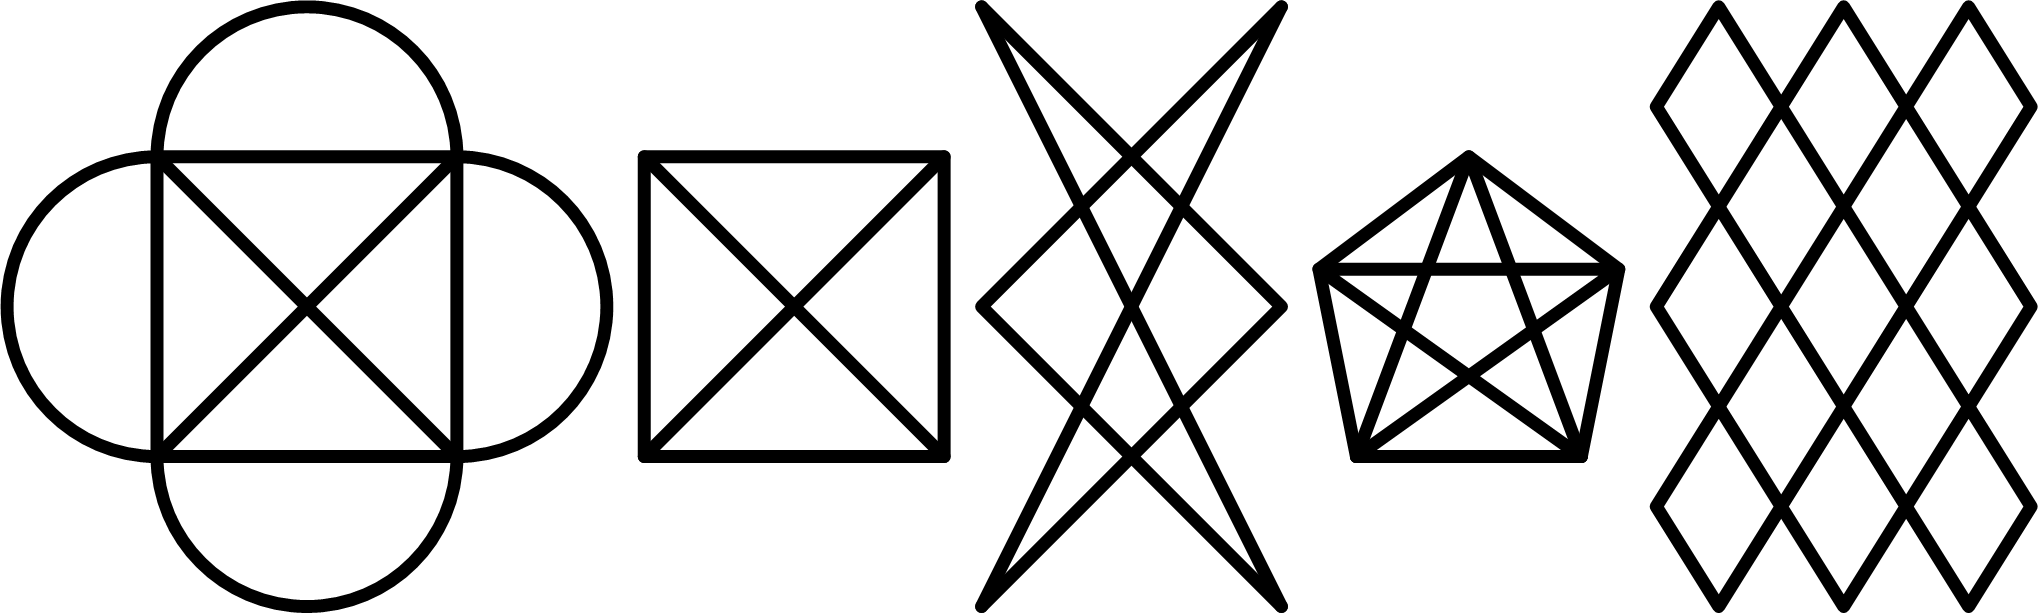
\includegraphics[width=0.7\textwidth]{fig/onlineFigure.png}
    \]
    
    \item Вычертить фигуру одним росчерком пера. При этом не обязательно маршрут, проходящий по всем ребрам, должен быть циклом, но пересекать ранее проведенную линию нельзя (как и проводить линию дважды). Доказать, что такой маршрут сущетвует, если все вершины имеют четную степень или, что только две вершины имеют нечетную степень.
    \[
        \begin{tabular}{ccccccccc}
            {\xymatrix{
                *{} \ar@{-}[r] \ar@{-}[dr] \ar@{-}[d]
                    &*{} \ar@{-}[d] \ar@{-}[dl] \ar@{-}@/^/[d]
                        \\
                *{} \ar@{-}[r]
                    &*{}                    
            }}
            &
            &
            {\xymatrix{
                *{} \ar@{-}[r] \ar@{-}@/^/[r] \ar@{-}@/_/[d] \ar@{-}[dr] \ar@{-}[d]
                    &*{} \ar@{-}[d] \ar@{-}[dl] \ar@{-}@/^/[d]
                        \\
                *{} \ar@{-}[r]
                    &*{}                    
            }}
            &
            &
            {\xymatrix{
                *{} \ar@{-}[r] \ar@{-}@/_/[d] \ar@{-}[d]
                    &*{} \ar@{-}[d] \ar@{-}@/^/[d]
                        \\
                *{} \ar@{-}[r]
                    &*{}                    
            }}
            &
            &
            {\xymatrix{
                *{} \ar@{-}[r] \ar@{-}@/_/[d] \ar@{-}[dr] \ar@{-}[d]
                    &*{} \ar@{-}[d] \ar@{-}@/^/[d]
                        \\
                *{} \ar@{-}[r]
                    &*{}                    
            }}
            &
            &
            {\xymatrix{
                *{} \ar@{-}[r] \ar@{-}@/^/[r] \ar@{-}[d] \ar@{-}[dr]
                    &*{} \ar@{-}[r] \ar@{-}[d] \ar@{-}[dr] \ar@{-}[dl]
                        &*{} \ar@{-}[d] \ar@{-}[dl]
                            \\
                *{} \ar@{-}[r]
                    &*{} \ar@{-}[r] \ar@{-}@/_/[r]
                        &*{} 
            }}
        \end{tabular}
    \]
    
    \item Найти гамильтоновы циклы в графах
    \[
        \begin{tabular}{cc}
            {
                \shorthandoff{"}
                \raisebox{\height}{
                    \(
                        \begin{xy}
                            \POS (0.00,15.00)*+[o][F-]{a}="a1"           \POS (14.27,4.64)*+[o][F-]{b}="b1"
                            \POS (8.82,-12.14)*+[o][F-]{c}="c1"          \POS (-8.82,-12.14)*+[o][F-]{d}="d1"
                            \POS (-14.27,4.64)*+[o][F-]{e}="e1"          \POS (0.00,7.00)*+[o][F-]{f}="a2"
                            \POS (6.66,2.16)*+[o][F-]{g}="b2"            \POS (4.11,-5.66)*+[o][F-]{h}="c2"
                            \POS (-4.11,-5.66)*+[o][F-]{i}="d2"          \POS (-6.66,2.16)*+[o][F-]{j}="e2"
                            \POS"a1" \ar @{-} "b1"            \POS"b1" \ar @{-} "c1"
                            \POS"c1" \ar @{-} "d1"            \POS"d1" \ar @{-} "e1"
                            \POS"e1" \ar @{-} "a1"            \POS"a2" \ar @{-} "b2"
                            \POS"b2" \ar @{-} "c2"            \POS"c2" \ar @{-} "d2"
                            \POS"d2" \ar @{-} "e2"            \POS"e2" \ar @{-} "a2"
                            \POS"a1" \ar @{-} "a2"            \POS"b1" \ar @{-} "b2"
                            \POS"c1" \ar @{-} "c2"            \POS"d1" \ar @{-} "d2"
                            \POS"e1" \ar @{-} "e2" 
                        \end{xy}        
                    \) 
                }
                \shorthandon{"}            
            }
            &
            \(\shorthandoff{"}
                \begin{xy}
                    \POS (0.00,40.00)*+[o][F-]{a}="l0"        \POS (0.00,28.57)*+[o][F-]{b}="l1"
                    \POS (9.38,22.86)*+[o][F-]{c}="l2"        \POS (18.75,22.86)*+[o][F-]{d}="l3"
                    \POS (25.00,28.57)*+[o][F-]{e}="l4"       \POS (25.00,17.14)*+[o][F-]{f}="l5"
                    \POS (6.25,11.43)*+[o][F-]{g}="l6"        \POS (9.38,0.00)*+[o][F-]{h}="l7"
                    \POS (-9.38,22.86)*+[o][F-]{i}="l8"       \POS (-18.75,22.86)*+[o][F-]{j}="l9"
                    \POS (-25.00,28.57)*+[o][F-]{k}="l10"     \POS (-25.00,17.14)*+[o][F-]{l}="l11"
                    \POS (-6.25,11.43)*+[o][F-]{m}="l12"      \POS (-9.38,0.00)*+[o][F-]{n}="l13"        
                    \POS "l0" \ar @{-} "l1"        \POS "l12" \ar @{-} "l6"
                    \POS "l13" \ar @{-} "l7"       \POS "l0" \ar @{-} "l4"
                    \POS "l0" \ar @{-} "l10"       \POS "l4" \ar @{-} "l5"
                    \POS "l10" \ar @{-} "l11"      \POS "l4" \ar @{-} "l3"
                    \POS "l10" \ar @{-} "l9"       \POS "l5" \ar @{-} "l3"
                    \POS "l11" \ar @{-} "l9"       \POS "l2" \ar @{-} "l3"
                    \POS "l8" \ar @{-} "l9"        \POS "l1" \ar @{-} "l2"
                    \POS "l1" \ar @{-} "l8"        \POS "l2" \ar @{-} "l6"
                    \POS "l8" \ar @{-} "l12"       \POS "l5" \ar @{-} "l7"
                    \POS "l11" \ar @{-} "l13"      \POS "l6" \ar @{-} "l7"
                    \POS "l12" \ar @{-} "l13"
                \end{xy}
                \shorthandon{"}            
            \)
        \end{tabular}
    \]

    \item Найти гамильтонов цикл в графе на рис. \ref{fig:graph:gamilton}.
    
    \item Найти изоморфизм графов
    \begin{enumerate}
        \item
        \(
            \shorthandoff{"}
            \begin{xy}
                \POS (0.00,15.00)*+[o][F-]{1}="a1"    \POS (11.73,9.35)*+[o][F-]{2}="b1"
                \POS (14.62,-3.34)*+[o][F-]{3}="c1"   \POS (6.51,-13.51)*+[o][F-]{4}="d1"
                \POS (-6.51,-13.51)*+[o][F-]{5}="e1"  \POS (-14.62,-3.34)*+[o][F-]{6}="f1"
                \POS (-11.73,9.35)*+[o][F-]{7}="g1"   \POS (40.00,15.00)*+[o][F-]{a}="a2"
                \POS (51.73,9.35)*+[o][F-]{b}="b2"    \POS (54.62,-3.34)*+[o][F-]{c}="c2"
                \POS (46.51,-13.51)*+[o][F-]{d}="d2"  \POS (33.49,-13.51)*+[o][F-]{e}="e2"
                \POS (25.38,-3.34)*+[o][F-]{f}="f2"   \POS (28.27,9.35)*+[o][F-]{g}="g2"
                \POS"a1" \ar @{-} "b1"    \POS"a1" \ar @{-} "c1"
                \POS"a1" \ar @{-} "f1"    \POS"a1" \ar @{-} "g1"
                \POS"b1" \ar @{-} "g1"    \POS"b1" \ar @{-} "c1"
                \POS"b1" \ar @{-} "d1"    \POS"c1" \ar @{-} "d1"
                \POS"c1" \ar @{-} "e1"    \POS"d1" \ar @{-} "e1"
                \POS"d1" \ar @{-} "f1"    \POS"e1" \ar @{-} "f1"
                \POS"e1" \ar @{-} "g1"    \POS"f1" \ar @{-} "g1"
                \POS"a2" \ar @{-} "b2"    \POS"a2" \ar @{-} "d2"
                \POS"b2" \ar @{-} "c2"    \POS"b2" \ar @{-} "e2"
                \POS"c2" \ar @{-} "d2"    \POS"c2" \ar @{-} "f2"
                \POS"d2" \ar @{-} "e2"    \POS"d2" \ar @{-} "g2"
                \POS"e2" \ar @{-} "f2"    \POS"e2" \ar @{-} "a2"
                \POS"f2" \ar @{-} "g2"    \POS"f2" \ar @{-} "b2"
                \POS"g2" \ar @{-} "a2"    \POS"g2" \ar @{-} "c2" 
            \end{xy}
            \shorthandon{"}
        \)
        \item
        \begin{tabular}{cc}
            {\entrymodifiers={+[o][F-]}
            \xymatrix@=6pt{
                a \ar@{-}[ddd] \ar@{-}[ddr] \ar@{-}[dr] \ar@{-}@/^21pt/[dddrrr]
                    &*{}
                        &*{}
                            &*{}
                                \\
                *{}
                    &b \ar@{-}[d] \ar@{-}[dr]
                        &*{}
                            &*{}
                                \\
                *{}
                    &n \ar@{-}[dl] \ar@{-}[drr]
                        &c \ar@{-}[dr]
                            &*{}
                                \\
                e \ar@{-}[rrr]
                    &*{}
                        &*{}
                            &d
            }}
            &
            {\entrymodifiers={+[o][F-]}
            \xymatrix@=6pt{
                1 \ar@{-}[dd] \ar@{-}[rr]  \ar@{-}[dr]
                    &*{}
                        &2 \ar@{-}[dr] \ar@{-}[dd] \ar@{-}[dl]
                            &*{}
                                \\
                *{}
                    &3 \ar@{-}[rr] \ar@{-}[dr] \ar@{-}[dl]
                        &*{}
                            &4 \ar@{-}[dl]
                                \\
                5 \ar@{-}[rr]
                    &*{}
                        &6
                            &*{}
            }}
        \end{tabular}
        
        \item
        \begin{tabular}{cc}
            {\entrymodifiers={+[o][F-]}
            \xymatrix@=6pt{
                1 \ar@{-}[dd] \ar@{-}[ddrr] \ar@{-}[rr]
                    &*{}
                        &2 \ar@{-}[ddll] \ar@{-}[dr] \ar@{-}[dr]  \ar@{-}[dd]
                            &*{}
                                \\
                *{}
                    &*{}
                        &*{}
                            &3 \ar@{-}[dl]
                                \\
                5
                    &*{}
                        &4 \ar@{-}[ll]
                            &*{}
            }}
            &
            {\entrymodifiers={+[o][F-]}
            \xymatrix@=6pt{
                a \ar@{-}[dd] \ar@{-}[ddrr] \ar@{-}[rr] \ar@{-}[drrr]
                    &*{}
                        &b \ar@{-}[ddll] \ar@{-}[dd]
                            &*{}
                                \\
                *{}
                    &*{}
                        &*{}
                            &c \ar@{-}[dl]
                                \\
                e
                    &*{}
                        &d \ar@{-}[ll]
                            &*{}
            }}
        \end{tabular}
    \end{enumerate}
    
    \item Выполнить укладку графов на плоскости
    \[
        \begin{tabular}{ccc}
            {
                \shorthandoff{"}
                \begin{xy}
                    \POS (0.00,15.00)*++[o][F-]{1}="a1"
                    \POS (14.27,4.64)*++[o][F-]{2}="b1"
                    \POS (8.82,-12.14)*++[o][F-]{3}="c1"
                    \POS (-8.82,-12.14)*++[o][F-]{4}="d1"
                    \POS (-14.27,4.64)*++[o][F-]{5}="e1"
                    \POS"a1" \ar @{-} "b1"
                    \POS"a1" \ar @{-} "c1"
                    \POS"a1" \ar @{-} "d1"
                    \POS"a1" \ar @{-} "e1"
                    \POS"b1" \ar @{-} "c1"
                    \POS"b1" \ar @{-} "d1"
                    \POS"b1" \ar @{-} "e1"
                    \POS"c1" \ar @{-} "e1"
                    \POS"d1" \ar @{-} "e1"
                \end{xy}        
                \shorthandon{"}            
            }        
            &
            \raisebox{1.5\height}{
                {\xymatrix{
                    1 \ar@{-}[d] \ar@{-}[dr] \ar@{-}[r]
                        &2 \ar@{-}[dl] \ar@{-}[d] \ar@{-}[dr] \ar@{-}[r]
                            &3 \ar@{-}[dll] \ar@{-}[dl] \ar@{-}[d]
                                \\
                    4 \ar@{-}[r]
                        &5 \ar@{-}[r]
                            &6                        
                }}
            }
            &
            {
                \shorthandoff{"}
                \begin{xy}
                    \POS (0.00,15.00)*++[o][F-]{1}="a2"
                    \POS (11.73,9.35)*++[o][F-]{2}="b2"
                    \POS (14.62,-3.34)*++[o][F-]{3}="c2"
                    \POS (6.51,-13.51)*++[o][F-]{4}="d2"
                    \POS (-6.51,-13.51)*++[o][F-]{5}="e2"
                    \POS (-14.62,-3.34)*++[o][F-]{6}="f2"
                    \POS (-11.73,9.35)*++[o][F-]{7}="g2"
                    \POS"a2" \ar @{-} "b2"
                    \POS"a2" \ar @{-} "d2"
                    \POS"b2" \ar @{-} "c2"
                    \POS"b2" \ar @{-} "e2"
                    \POS"c2" \ar @{-} "d2"
                    \POS"c2" \ar @{-} "f2"
                    \POS"d2" \ar @{-} "g2"
                    \POS"e2" \ar @{-} "f2"
                    \POS"e2" \ar @{-} "a2"
                    \POS"f2" \ar @{-} "g2"
                    \POS"f2" \ar @{-} "b2"
                    \POS"g2" \ar @{-} "a2"
                    \POS"g2" \ar @{-} "c2" 
                \end{xy}
                \shorthandon{"}
            }
        \end{tabular}
    \]
    
    \item Определите цикломатические числа в приведенных графах. Сколько всего циклов можно выделить в этих графах? Выделите цикловой базис, разложите все возможные циклы в этом базисе.
    
    \begin{tabular}{ccc}
        \(    
            {\xymatrix{
                1 \ar@{-}[d] \ar@{-}[dr] \ar@{-}[r]
                    &2 \ar@{-}[dl] \ar@{-}[d]
                        \\
                4 \ar@{-}[r]
                    &3 
            }}
        \)   
        &        
        \(    
            {\xymatrix@=7pt{
                1 \ar@{-}[dd] \ar@{-}[dr] \ar@{-}[rr]
                    &*{}
                        &2 \ar@{-}[dl] \ar@{-}[dd]
                            \\
                *{}
                    &5 \ar@{-}[dr]
                        &*{}
                            \\
                4 \ar@{-}[rr]
                    &*{}
                        &3 
            }}
        \)
        &
        \(    
            {\xymatrix@=7pt{
                1 \ar@{-}[dd] \ar@{-}[dr] \ar@{-}[rr]
                    &*{}
                        &2 \ar@{-}[dl] \ar@{-}[dd]
                            \\
                *{}
                    &5 \ar@{-}[dr] \ar@{-}[dl]
                        &*{}
                            \\
                4 \ar@{-}[rr]
                    &*{}
                        &3 
            }}
        \)
    \end{tabular}
    
\end{enumerate}
 %Графы
    \chapter{Индукция и рекурсия}

%rec: label prefix
Чтобы понять что такое \emph{рекурсия}, нужно понять, что такое \emph{рекурсия}. Для углубленного изучения вопросов, касающихся индукции и рекурсии, рекомендуются \cite{bib:haggard:discrmathprogrammer,bib:miller:secParAlghorithm,bib:hopkroft:automateIntro}.


\section{Индукция и рекурсия}

Термины \emph{индукция} и \emph{рекурсия} часто употребляются вместе. Следует провести границу между ними.

Математическая \emph{индукция} --- это метод рассуждений (доказательства) от частного к общему. То есть утверждения об общем случае выводятся(\emph{индуцируются}) из очевидных частных случаев --- \emph{фактов}. Базовый принцип математической индукции заключается в следующем.
\begin{enumerate}
    \item \emph{Базис}. Показана истинность утверждения $P(i)$, где $i\in\mathbb{N}$. Обычно $i=0$ или $i=1$. Но в общем случае может быть и так, что $P(j)$ ложно для $j<i$.
    \item \emph{Индуктивный переход}. Для произвольного $n\geq i,n\in\mathbb{N}$ доказано, что из истинности $P(n)$ следует истинность $P(n+1)$. Т.е. доказываем $P(n)\Rightarrow P(n+1)$.
\end{enumerate}

\begin{exampl}
    Задача. Доказать, что 
    \[
        \sum_{i=0}^{n}i^2=\frac{2n^3+3n^2+n}{6}.
    \]
\end{exampl}
\begin{proof}[Решение]
    В качестве базисного случая возьмем $n=0$. Видно, что равенство выполняется.
    
    По индукции предположим $n\geq 0$. Подставим вместо $n$ значение $n+1$:
    \[
        \sum_{i=0}^{n+1}i^2=\frac{2n^3+9n^2+13n+6}{6}.
    \]
    
    Справедливо:
    \[
        \begin{split}
            \sum_{i=0}^{n+1}i^2=(n+1)^2+\sum_{i=0}^{n}i^2=\\
            =(n+1)^2+\frac{2n^3+3n^2+n}{6}=\frac{2n^3+9n^2+13n+6}{6}.
        \end{split}
    \]
    Следовательно, можно сделать вывод, что доказываемое утверждение спрведливо для всех $n$.
\end{proof}

Общая форма математической индукции заключается в следующем.
\begin{enumerate}
    \item \emph{Базис}. Показана истинность утверждений $P(i),P(i+1),\ldots,P(j)$, где $i,j\in\mathbb{N},j>i$.
    \item \emph{Индуктивный переход}. Для $n\geq j$ при доказательстве истинности $P(n+1)$ можно использовать не только $P(n)$, но и все утверждения $P(i),P(i+1),\ldots,P(n)$.
\end{enumerate}

\begin{exampl} 
    Задача. Доказать $P(n)$: если $n\geq 8$, то $n$ можно представить суммой троек и пятерок.
\end{exampl}
\begin{proof}[Решение]
    Базис: 8=3+5, 9=3+3+3, 10=5+5. Индуктивный переход. Предполагаем истинность $P(8),P(9),P(10),\ldots,P(n)$. Доказывая $P(n+1)$ вычтем $3$ из $n+1$. Заметим, что $P(n-2)$ истинно. То есть $n-2$ представимо суммой $3k+5m$ пятерок и троек, а стало быть и $n+1$ также представимо, так как $n+1=3(k+1)+5m$.
\end{proof}

\emph{Рекурсия} в общем случае --- это \emph{самоподобие}. Таким свойством самоподобности, кроме всех прочих объектов, могут обладать математические формулы, данные и алгоритмы. 

Примером рекурсивной (самоподобной) структуры данных может быть список.
\begin{exampl} 
    Пусть имеются атомарные (неделимые) типы данных, такие как: число, строка, символ и т.д. Список можно определить так:
    \begin{enumerate}
        \item любой атом есть список;
        \item если $l_1,l_2,\ldots,l_n$ --- списки, то $(l_1,l_2,\ldots,l_n)$ есть список;
        \item ничто другое не является списком.
    \end{enumerate}
    
    Пример списка: $(1,(2,(3,4)),5)$.\qed
\end{exampl}

Рекурсивный алгоритм решения задачи обычно выполняется так:
\begin{enumerate}
    \item если задача тривиальна, то выдается решение и алгоритм завершается;
    \item в противном случае исходная задача разбивается на подзадачи меньшей размерности;
    \item каждая подзадача, решается тем же алгоритмом, что и исходная задача (то есть \emph{рекурсивно});
    \item решения подзадач объединяются так, чтобы получить решение исходной задачи.
\end{enumerate}

Важно отметить следующие особенности рекурсивных алгоритмов.
\begin{enumerate}
    \item Существование одного или нескольких базовых случаев для решаемой задачи. Решение базового случая тривиально и может быть получено сразу. Именно к базовым случаям в конечном итоге сводится решение любой исходной задачи.
    \item Существование способа сведения исходной задачи к решению подобных ей подзадач и получения результата исходной задачи на основе результатов подзадач.
\end{enumerate}

Индуктивные рассуждения часто используются для обоснования корректности рекурсивных алгоритмов. Самоподобные (рекурсивные) логические рассуждения называются индуктивными.


\section{Реккурентные математические формулы}

Выражающиеся сами через себя математические формулы называют \emph{реккурентными}. Вычисление значений таких формул для больших $n$ занимает слишком много времени, поэтому представляет интерес возможность свести реккурентность к <<замкнутой>> (аналитической) формуле, то есть к вычислимой непосредственно. Для рассматриваемых ниже реккурентных формул первого и второго рода порой удается получить решение в <<замкнутой форме>>.


\subsection{Реккурентные формулы первого рода}

В качестве примера рассмотрим задачу о Ханойских башнях.
\begin{exampl} 
    Задача. На первый из трех алмазных стержней насажены золотые диски в количестве 64-х штук. Все диски разного диаметра и диск меньшего диаметра лежит на диске большего диаметра. Требуется переместить диски на третий стержень в том же порядке, в каком они находятся на первом, перекладывая за раз по одному диску. Второй столбик используется как вспомогательный. В процессе перемещения нельзя класть больший диск на меньший\footnote{По легенде задача поставлена Всевышним перед жрецами, которые в настоящий момент над ней должны работать в несколько смен днем и ночью, и как только они закончат, наступит конец света. Хотелось бы прикинуть: стоит ли вообще браться за дальнейшее изучение рекурсии?}.
\end{exampl}
\begin{proof}[Решение]
    Возьмем меньшее количество дисков и убедимся, что задача решаема (см. рис \ref{fig:rec:hanoi}). Для одного диска решение очевидно. Для двух тоже.

    \begin{figure}
        \centering
        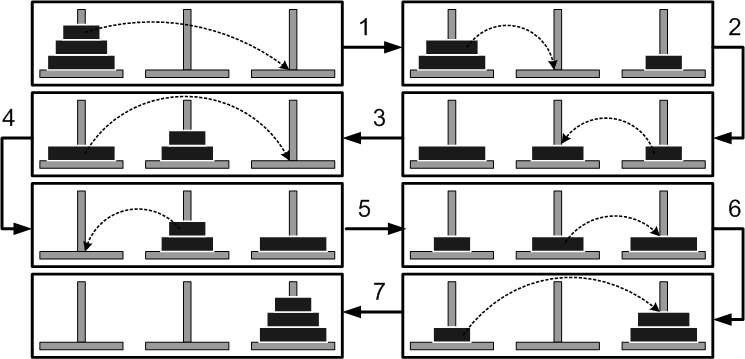
\includegraphics[width=0.67\textwidth]{fig/hanoi.png}
        \caption{Ханойские башни (три диска)}\label{fig:rec:hanoi}
    \end{figure}

    Попробуем обобщить на произвольное количество дисков. Для того, чтобы перенести $n$ дисков на третий столбик нужно $n-1$ верхних дисков сложить на второй столбик (очевидно, это можно сделать), оставшийся на первом столбике диск переложить на третий, и на него переместить $n-1$ дисков со второго (см. рисунок \ref{fig:rec:hanoi4}).

    \begin{figure}
        \centering
        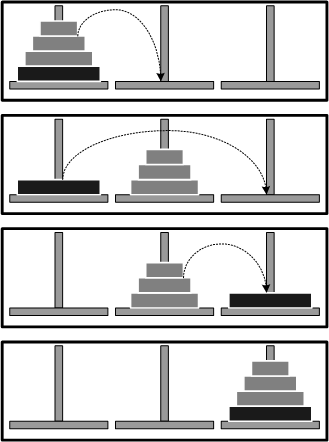
\includegraphics[width=0.27\textwidth]{fig/hanoi4.png}
        \caption{Ханойские башни (обобщение)}\label{fig:rec:hanoi4}
    \end{figure}

    Стало быть, если $T(n)$ --- количество перекладываний для переноса $n$ дисков, имеем: перенос на второй столбик потребует $T(n-1)$ перекладываний, одно перекладывание с первого на третий, и финальные $T(n-1)$ перекладываний на третий. $T(n)=2\cdot T(n-1) + 1$. В реккурентной форме:
    \[
        T(n)=
        \begin{cases}
            0,                  & n=0, \text{\emph{База рекурсии}},\\
            2\cdot T(n-1) + 1,  & n>0, \text{\emph{Реккурентный переход}}.
        \end{cases}
    \]

    Теперь можно легко двигаться от базы, получая:
    \[
        \begin{array}[c]{c||c|c|c|c|c|c|c|c|c|}
            \hline
            n       &0  &1  &2  &3  &4  &5  &6  &7   &8\\ \hline
            T(n)    &0  &1  &3  &7  &15 &31 &63 &127 &255\\ \hline
        \end{array}
    \]

    Тем не менее это неудобно --- слишком много последовательных решений. Хотелось бы сразу, не впадая в рекурсивный спуск, ответить сколько же нужно перекладываний для перемещения $n$ дисков? Пусть $K(n)=T(n)+1$.

    \[
        \begin{split}
                        T(n)+1=2\cdot T(n-1) + 2\Rightarrow\\
            \Rightarrow T(n)+1=2\cdot (T(n-1) + 1)\Rightarrow\\
            \Rightarrow K(n)=2\cdot (K(n-1))\Rightarrow\\
            \Rightarrow K(n)=2\cdot 2\cdot (K(n-2))\Rightarrow\\
            \Rightarrow K(n)=\underbrace{2\cdot 2\cdot\ldots\cdot 2\cdot2}_{n}\cdot K(0) = 2^n\Rightarrow\\
            \Rightarrow T(n)=K(n)-1=2^n-1.
        \end{split}
    \]

    Решение задачи о Ханойских башнях\footnote{Возвращаясь к теме конца света: если Всевышний запретил жрецам использовать роботов, то шанс разобраться с рекурсией есть}: $T(64)=2^{64}-1=18446744073709551615$ перекладываний.
\end{proof}

К сожалению, не всегда получается перейти от реккурентной формулы к простой аналитической, как это сделано в задаче о Ханойских башнях. В общем случае реккурентные формулы первого рода определяются так:
\begin{equation}
    \label{eq:rec:rec1type}
    T(n)=
    \begin{cases}
        f(k),                  & n=k, \text{\emph{База рекурсии}},\\
        c\cdot T(n-1) + f(n),  & n>k, \text{\emph{Реккурентный переход}},
    \end{cases}
\end{equation}
где $n,k\in\mathbb{N}$, $c$ --- константа, а $f$ --- ненулевая функция от $n$ при $n\geq k$.

При этом формуле \eqref{eq:rec:rec1type} эквивалентна сумма
\begin{equation}
    \label{eq:rec:rec1typeSum}
    T(n)=\sum_{i=k}^{n}c^{n-i}\cdot f(i).
\end{equation}

Это можно доказать по индукции, или выполнив $n-k$ подстановок вместо $T(n-1)$ в выражении реккурентного перехода формулы \eqref{eq:rec:rec1type}. Программисту эта эквивалентность дает возможность уйти от рекурсивной подпрограммы к обычному циклу.


\subsection{Реккурентные формулы второго рода}

Примером реккурентных формул второго рода являются числа Фибоначчи, определяемые рекурсивно так:
\begin{equation}
    \label{eq:rec:fibonacci}
    f(n)=
    \begin{cases}
        0,              &n=0\\
        1,              &n=1\\
        f(n-1)+f(n-2),  &n\geq 2.
    \end{cases}
\end{equation}

В общем случае реккурентные формулы второго рода имеют вид
\begin{equation}
    f(n)=
    \begin{cases}
        a_{k},                          &n=k\\
        a_{k+1},                        &n=k+1\\
        b_1\cdot f(n-1)+b_2\cdot f(n-2),&n\geq k+2,
    \end{cases}
\end{equation}
где $b_1,b_2$ --- константы.

Алгоритм получения аналитического решения для данных соотношений следующий.
\begin{enumerate}
    \item Предположив $f(n)=c^n$, подставить выражение в формулу реккурентного перехода $f(n)=b_1\cdot f(n-1)+b_2\cdot f(n-2)$: 
    \[
        \begin{split}
                        c^n-b_1\cdot c^{n-1}-b_2\cdot c^{n-2} = 0\Rightarrow\\
            \Rightarrow c^{n-2}\cdot(c^2 - b_1\cdot c - b_2) = 0.
        \end{split}
    \]
    
    \item Решить\footnote{Напомним, что для квадратного уравнения $ax^2+bx+c=0$ решениями будут $x_{1,2}=\frac{-b\pm\sqrt{b^2-4ac}}{2a}$} характеристическое уравнение $c^2 - b_1\cdot c - b_2 = 0$ относительно $c$, получив корни $c_1,c_2$.
    
    \item $f(n)$ будет имет следующее аналитическое выражение:
    \begin{equation}
        \label{eq:rec:rec2typeAnalytic}
        f(n)=D_1\cdot {c_1}^n + D_2\cdot{c_2}^n,
    \end{equation}
    где $D_1,D_2$ --- параметры, которые необходимо найти.
    
    \item Воспользоваться начальными условиями, чтобы построить систему уравнений
    \[
        \begin{cases}
            a_k     = D_1\cdot {c_1}^k + D_2\cdot{c_2}^k\\
            a_{k+1} = D_1\cdot {c_1}^{k+1} + D_2\cdot{c_2}^{k+1}\\            
        \end{cases}
    \]
    
    Решить систему относительно двух неизвестных $D_1,D_2$.
    
    \item Решением реккурентности будет формула \eqref{eq:rec:rec2typeAnalytic}.
\end{enumerate}

\begin{exampl}
    Найти аналитическое решение для поиска чисел Фибоначчи (см. формулу \eqref{eq:rec:fibonacci}).
\end{exampl}
\begin{proof}[Решение] 
    Применяя алгоритм:
    
    \begin{enumerate}
        \item Характеристическое уравнение $c^2-c-1=0$.
        \item Корни характеристического уравнения: $c_1=\frac{1+\sqrt{5}}{2},c_2=\frac{1-\sqrt{5}}{2}$
        \item Решая систему уравнений:
        \[
            \begin{cases}
                0=D_1 + D_2\\
                1=D_1\frac{1+\sqrt{5}}{2} + D_2\frac{1-\sqrt{5}}{2},
            \end{cases}
        \]
        получаем решения $D_1=\frac{1}{\sqrt{5}}, D_2=-\frac{1}{\sqrt{5}}$.
        \item Получено $f(n)=\frac{1}{\sqrt{5}}(\frac{1+\sqrt{5}}{2})^n-\frac{1}{\sqrt{5}}(\frac{1-\sqrt{5}}{2})^n$. Следовательно $n$-е число Фибоначчи можно найти, не прибегая к рекурсии.
    \end{enumerate}
\end{proof}


\section{Рекурсивные структуры данных и вычисления}

\emph{Дерево} --- частный случай графа, может быть определено рекурсивно.
\begin{enumerate}
    \item Одиночный узел $v$ есть дерево, и $v$ является корнем полученного дерева.
    \item Если $t_1,t_2,\ldots,t_n$ --- деревья, а $v$ одиночный узел, то в результате соединения корня каждого из деревьев $t_1,t_2,\ldots,t_n$ с узлом $v$ будет получено дерево с корнем $v$.
    \item других правил образования дерева нет.
\end{enumerate}

По соглашению будем рисовать дерево так, чтобы корень располагался выше остальных узлов дерева. Дерево настолько универсальная структура, что им можно представить практически любой рекурсивно определяемый объект.
\begin{exampl} Задача.
    Математическую формулу, состоящую из литералов (чисел), имен переменных и знаков арифметических опереций (например, $+$, $*$) можно определить рекурсивно.
    \begin{enumerate}
        \item Отдельный литерал есть математическая формула.
        \item Отдельное имя переменной есть математическая формула.
        \item Если $A$ и $B$ --- математические формулы, то и $(A+B)$ и $(A*B)$ --- математические формулы.
    \end{enumerate}
    Построить деревья, соответствующие выражениям $1+2*3$ и $(1+2)*3$.
\end{exampl}
\begin{proof}[Решение]
    Дерево, соответствующее формуле будем строить так:
    \begin{enumerate}
        \item Отдельному литералу сопоставляется дерево из одного узла (корня), который содержит литерал.
        \item Отдельному имени переменной сопоставляется дерево из одного узла (корня), который содержит имя переменной.
        \item Если $A$ и $B$ --- математические формулы, которым соответствуют деревья $T_A$ и $T_B$, то
        формуле $(A+B)$ соответствует дерево с узлом (корнем) $v$, который содержит символ $+$ и соединяется с корнями деревьев $T_A$ и $T_B$. Дерево для формулы $(A*B)$ определяется аналогично.
    \end{enumerate}
    
    \begin{figure}
        \centering
        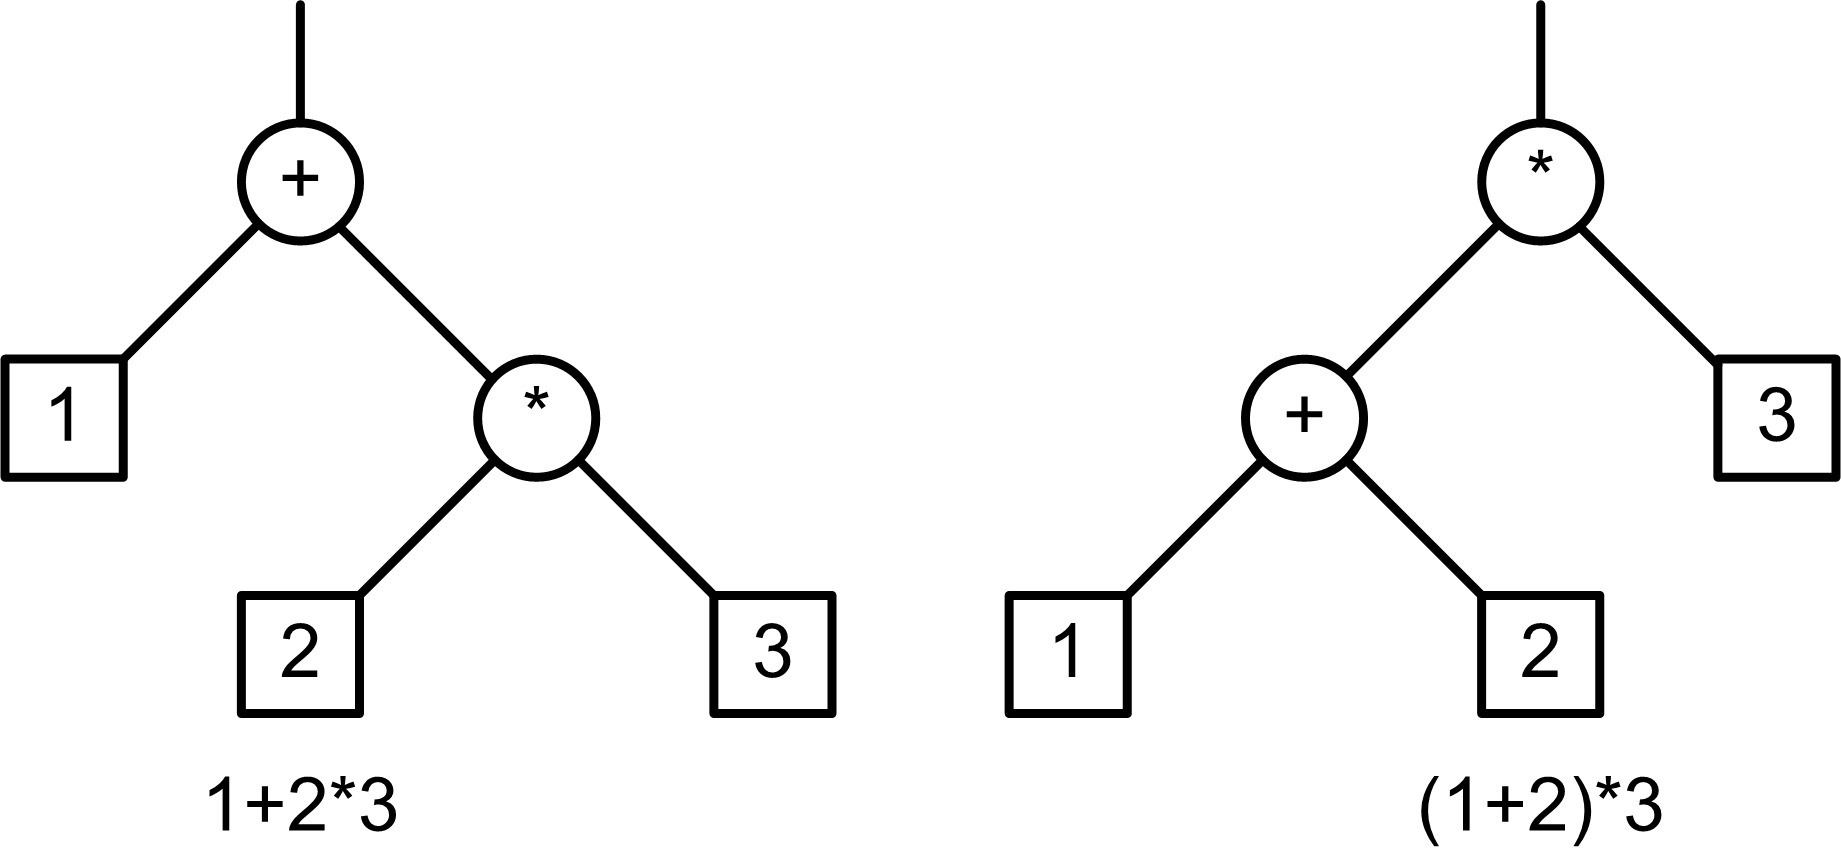
\includegraphics[width=0.67\textwidth]{fig/formulaeTree.png}
        \caption{Пример соответствия дерева формуле}\label{fig:rec:formulaeTree}
    \end{figure}
    
    Так как по принятым соглашениям умножение выполняется раньше, то формуле $1+2*3$ эквивалентна формула $(1+(2*3))$, а формуле $(1+2)*3$ --- формула $((1+2)*3)$. Соответствующие деревья приведены на рисунке \ref{fig:rec:formulaeTree}.
\end{proof}

Привычная запись формул называется \emph{инфиксной}. Проводить вычисления по инфиксной записи не удобно: на порядок действий влияют, например, приоритет, скобки и ассоциативнось операций. Более удобной для вычислений является запись \emph{постфиксная} запись\footnote{Постфиксную запись часто называют польской записью}, не содержащая ни скобок, ни других условностей. Получение постфиксной записи формулы из соответствующего дерева приведено в псевдокоде \ref{alg:rec:postfix}. Псевдокод для инфиксной и постфиксной форм будет отличаться от псевдокода \ref{alg:rec:postfix} лишь в строке \ref{alg:l:rec:sOrder}.
\begin{itemize}
    \item Для инфиксной формы: $s\gets \text{<<(>>}s_1s_3s_2\text{<<)>>}$.
    \item Для префиксной формы: $s\gets s_3s_1s_2$.
\end{itemize}

\begin{algorithm}
    \caption{Постфиксная запись формулы $postfix(t)$}\label{alg:rec:postfix}
    \begin{algorithmic}[1]
        \REQUIRE{$t$ --- дерево, соответствующее формуле. $t.text$ --- содержимое узла, $t.left$ --- левое поддерево, $t.right$ --- правое поддерево}
        \ENSURE{$s$ --- постфиксная запись формулы}

        \IF{$t$ --- отдельный узел}
            \STATE{$s\gets t.text$}
        \ELSE[$t$ содержит поддеревья]
            \STATE{$s_1\gets postfix(t.left)$} 
            \STATE{$s_2\gets postfix(t.right)$}
            \STATE{$s_3\gets t.text$}
            \STATE{$s\gets s_1s_2s_3$}\label{alg:l:rec:sOrder}
        \ENDIF
        \RETURN{$s$}
    \end{algorithmic}
\end{algorithm}

Рекурсивный обход дерева формулы $1+2*3$ и получение префиксной, инфиксной и постфиксной форм представлен на рисунке \ref{fig:rec:XfixForms}.

\begin{figure}
    \centering
    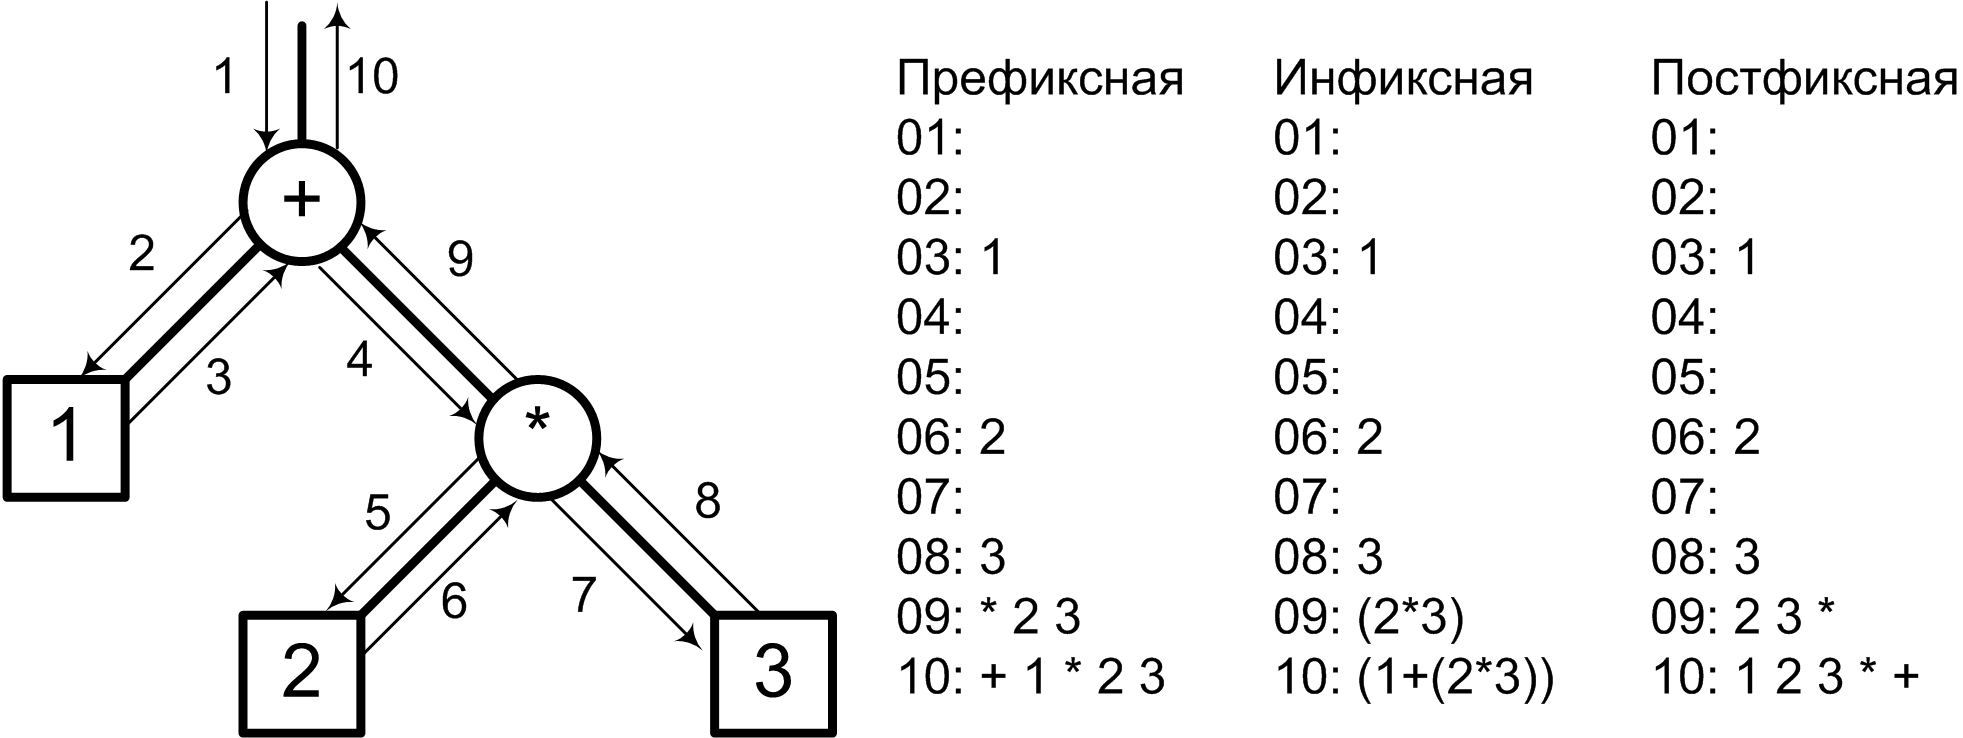
\includegraphics[width=0.87\textwidth]{fig/XfixForms.png}
    \caption{Префиксная, инфиксная и постфиксная запись $1+2*3$}
    \label{fig:rec:XfixForms}
\end{figure}

С вычислением постфиксной записи формулы спрвляется \emph{стековая машина}\footnote{Популярная виртуальная машина java является стековой}. \emph{Стек} --- это магазинная память, доступ к которой осуществляется с помощью двух команд:
\begin{enumerate}
    \item $push(X)$ --- поместить значение $X$ на вершину стека;
    \item $pop()$ --- изьять с вершины стека значение и вернуть его; $Y=pop()$ --- в $Y$ получим значение с вершины стека.
\end{enumerate}

Стек работает по принципу <<последним пришел, первым ушел>> (LIFO --- Last In First Out). То есть элементы, помещенные в стек командами $push$ будут извлечены в обратном порядке командами $pop$.

Алгоритм работы стековой машины для интерпретации постфиксной записи будет таким.
\begin{itemize}
    \item Вход: программа в виде выражения в постфиксной (обратной польской) записи.
    \item Выход: результат вычисления выражения.
    \item Шаги.
    \begin{enumerate}
        \item Программа просматривается посимвольно слева направо. Указатель текущего символа $ip$ устанавливается на начало программы.
        
        \item \label{en:rec:stackSee}Если текущий символ --- число или идентификатор переменной (обозначим и то и другое $X$), то соответствующее значение помещается в стек: $push(X)$, указатель текущего символа смещается вправо и выполняется перход на шаг \ref{en:rec:stackSee}. Иначе --- переход к следующему шагу.
        
        \item Если текущий символ выражения --- символ операции, то из стека командами $pop()$ извлекается необходимое количество аргументов, над которыми выполняется соответствующая операция, результат $R$ помещается в стек: $push(R)$, а указатель текущего символа сдвигается вправо и выполняется переход на шаг \ref{en:rec:stackSee}. Иначе --- к следующему шагу.
        
        \item Завершение работы. Достигнут конец выражения, а на вершине стека получен результат: $R=pop()$.
    \end{enumerate}
\end{itemize}

Работа стековой машины проиллюстрирована на рисунке \ref{fig:rec:stackMachine}.

\begin{figure}
    \centering
    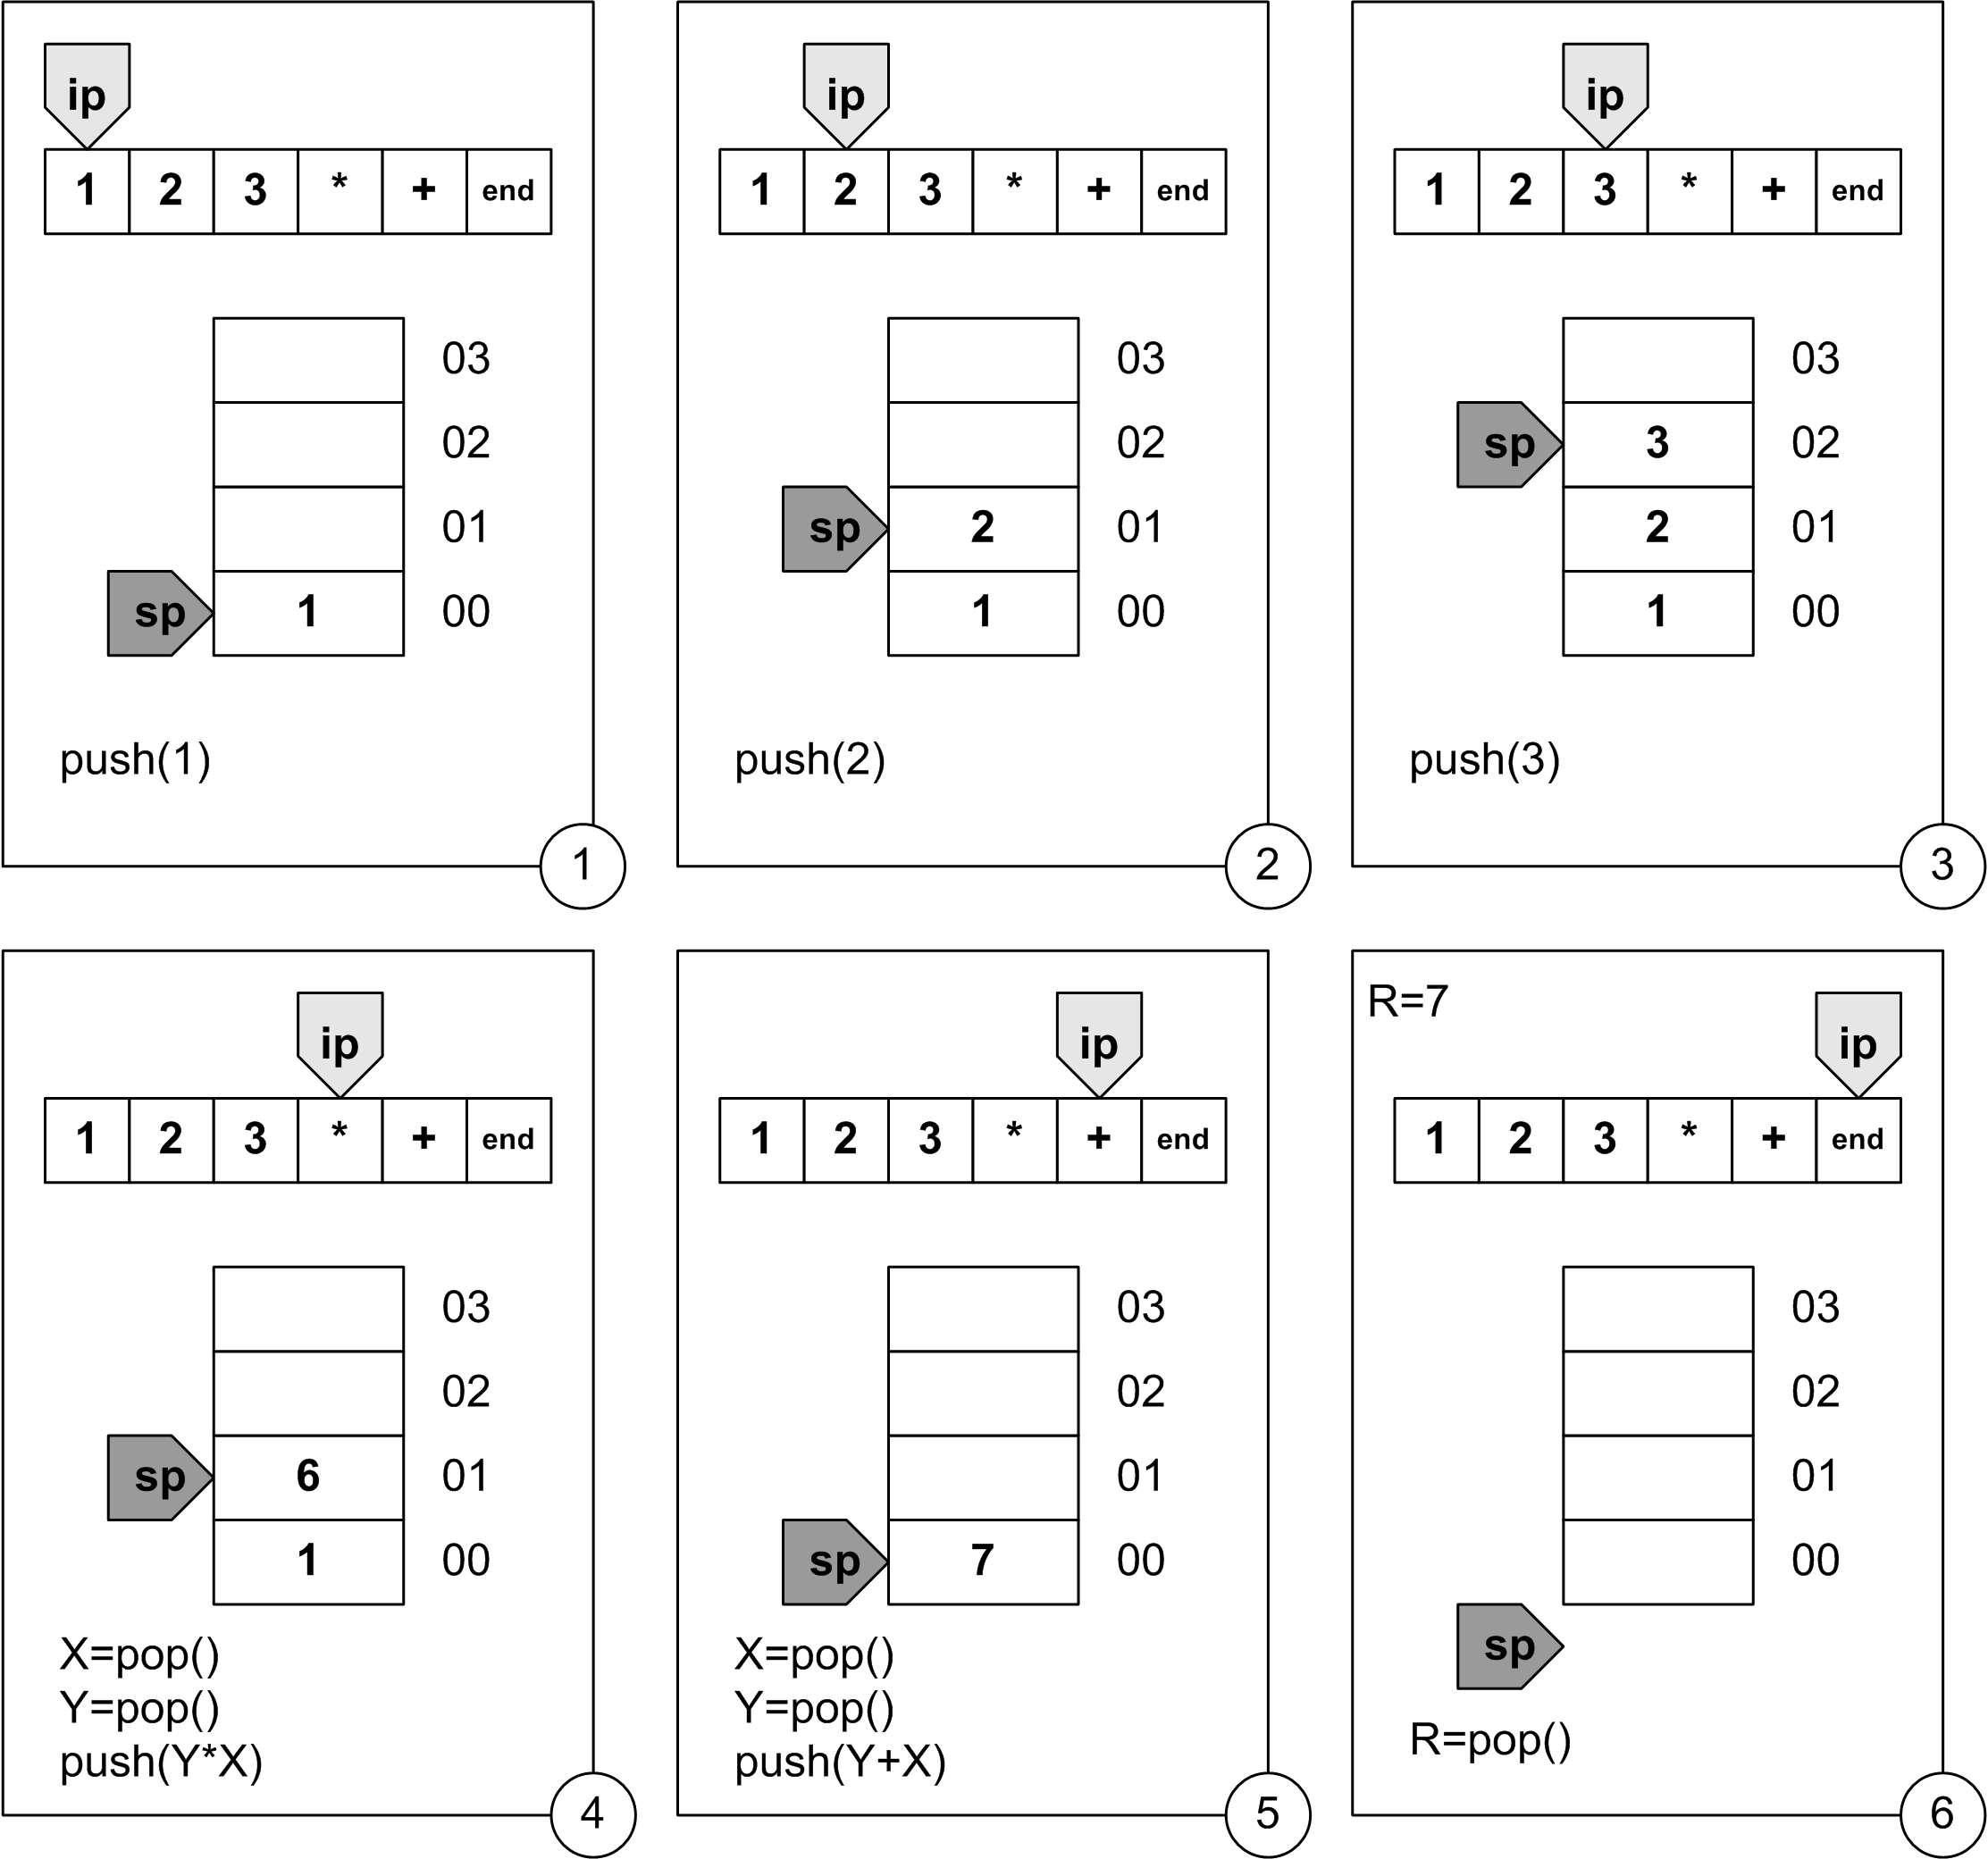
\includegraphics[width=0.87\textwidth]{fig/stackMachine.png}
    \caption{Стековая машина интерпретирует постфиксную запись}
    \label{fig:rec:stackMachine}
\end{figure}


\section{Представление деревьев в ЭВМ}

В качестве примера выбрано дерево, представленное на рисунке \ref{fig:rec:treeRepBase}. Дальнейшие примеры представления деревьев эквивалентны ему.
\begin{figure}
    \centering
    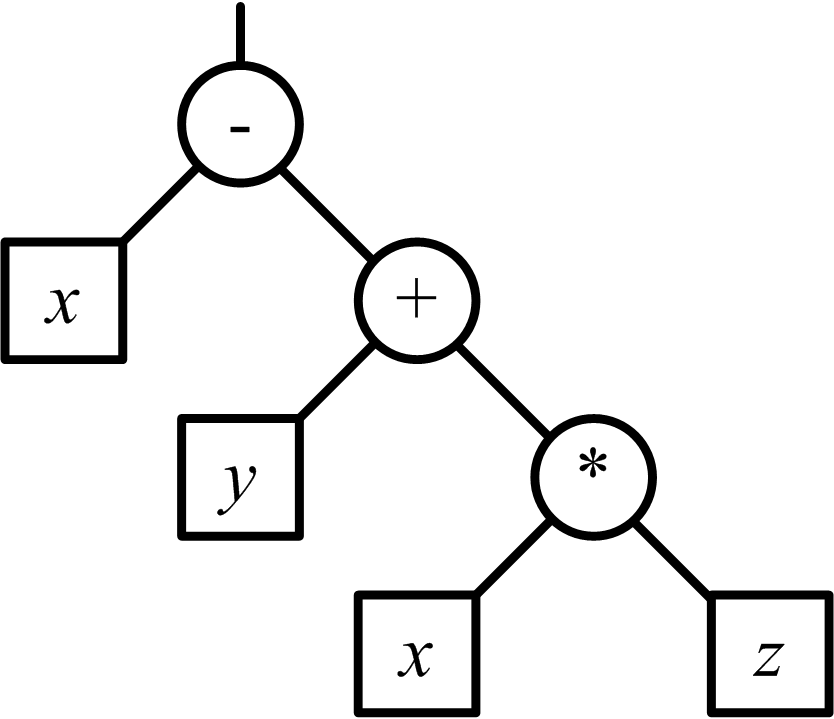
\includegraphics[width=0.3\textwidth]{fig/treeRepBase.png}
    \caption{Дерево для $x-(y+x*z)$}
    \label{fig:rec:treeRepBase}
\end{figure}


\subsection{Представление деревьев в памяти}

Дерево в памяти ЭВМ очевидным способом представляется структурой $T$, которая содержит полезные данные узла-корня и мaссив \emph{ссылок} на структуры $T$. В памяти, поддеревья, состоящие из одного узла, содержат специальное значение <<пустой>> ссылки (null) во всех элементах массива ссылок на структуры $T$. В программе дерево представлено ссылкой на корневую структуру $T$ дерева. См. рис. \ref{fig:rec:treeRepList}. 
\begin{figure}
    \centering
    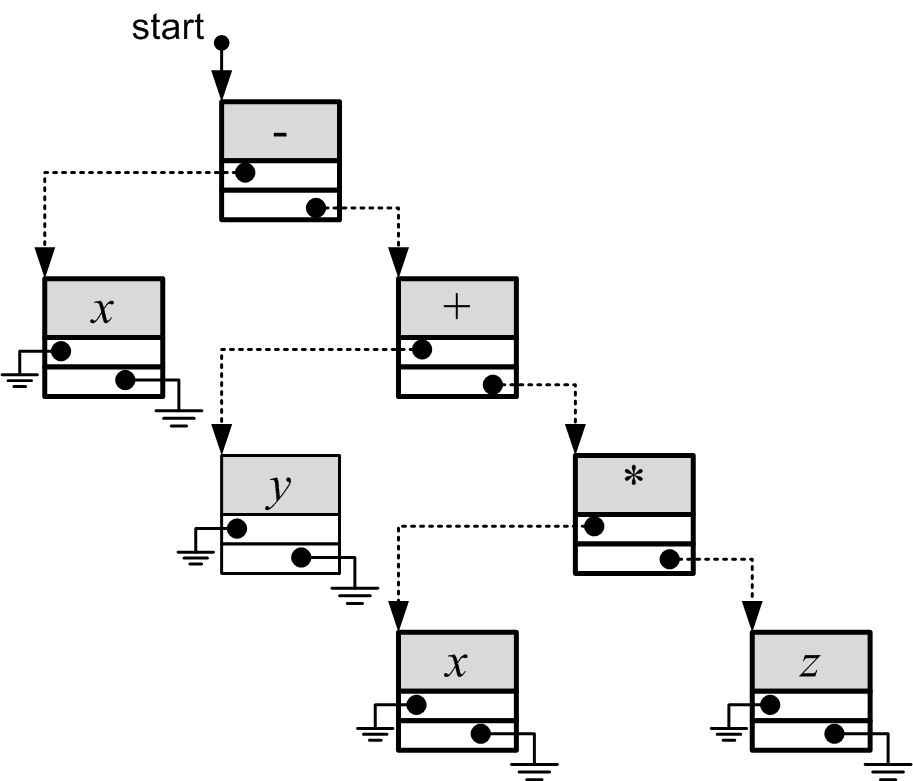
\includegraphics[width=0.57\textwidth]{fig/treeRepList.png}
    \caption{Представление дерева двусвязным списком}
    \label{fig:rec:treeRepList}
\end{figure}

В ряде задач требуется представить эквивалент дерева в виде линейного списка или массива, чтобы упростить обход. В этом случае можно предложить следующее представление. Модифицировав псевдокод \ref{alg:rec:postfix} постфиксной записи так, чтобы выражения выводились в скобках, для дерева на рис. \ref{fig:rec:treeRepBase} получим следующий список:
\[
    ((x)((y)((x)(z)*)+)-).
\]
В памяти его удобно представить массивом (списком см. рис. \ref{fig:rec:treeRepLinearList}) структур $N=\langle l,n,r\rangle$, где $n$ --- значение узла, $l$ --- количество открывающих скобок слева, $r$ --- количество закрывающих скобок справа:
\[
    \langle 2,x,1\rangle,
    \langle 2,y,1\rangle, 
    \langle 2,x,1\rangle,
    \langle 1,z,1\rangle,
    \langle 0,*,1\rangle,
    \langle 0,+,1\rangle,
    \langle 0,-,1\rangle.
\]

\begin{figure}
    \centering
    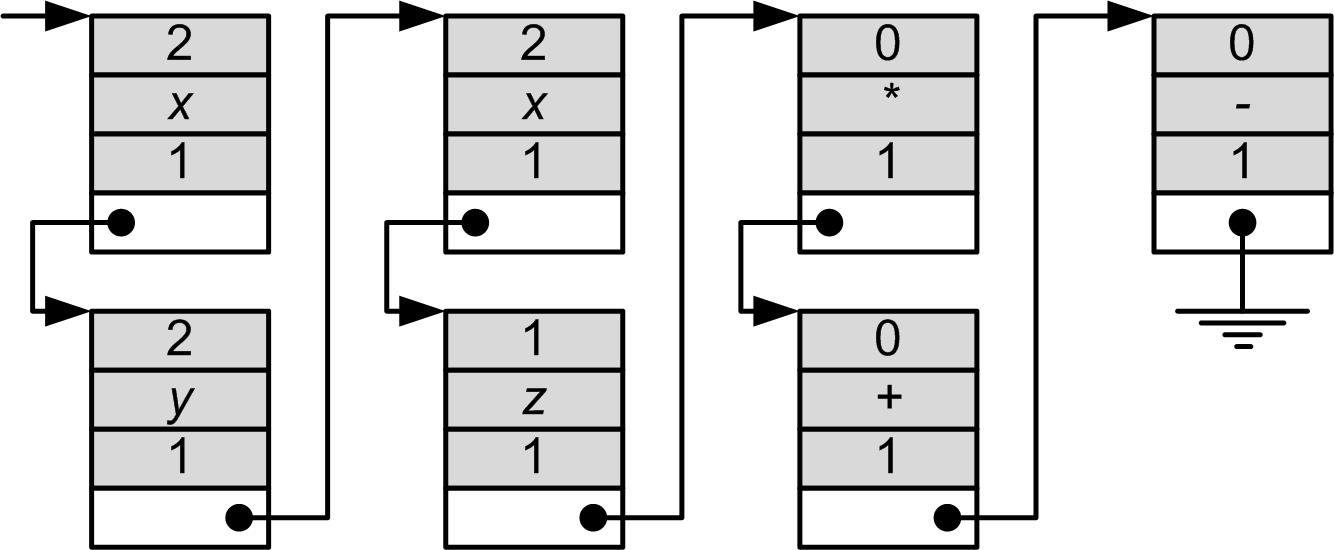
\includegraphics[width=0.57\textwidth]{fig/treeRepLinearList}
    \caption{Представление дерева линейным списком}
    \label{fig:rec:treeRepLinearList}
\end{figure}

Конечно, возможны и другие представления деревьев в памяти.


\subsection{Представление деревьев в реляционных таблицах}

Таблицы реляционных баз данных предназначены для хранения отношений, но иногда требуется представить в табличном виде дерево. Наиболее простой способ это сделать (см. рис. \ref{fig:rec:treeRepParent}) --- проиндексировать узлы дерева и в соответствующей таблице определить поля:
\begin{itemize}
    \item идентификатор узла (id);
    \item значение узла (text);
    \item идентификатор родительского узла (pid).
\end{itemize}

При этом идентификатор родительского узла корня совпадает с его собственным идентификатором.
\begin{figure}
    \centering
    \begin{tabular}{cc}
        \begin{tabular}{|c|c|c|}
            \hline\hline
            id  &text   &pid \\
            \hline\hline
            1   &-      &1 \\ \hline
            2   &x      &1 \\ \hline
            3   &+      &1 \\ \hline
            4   &y      &3 \\ \hline
            5   &*      &3 \\ \hline
            6   &x      &5 \\ \hline
            7   &z      &5 \\ \hline
        \end{tabular}
        &\raisebox{-.5\height}{
            \fbox{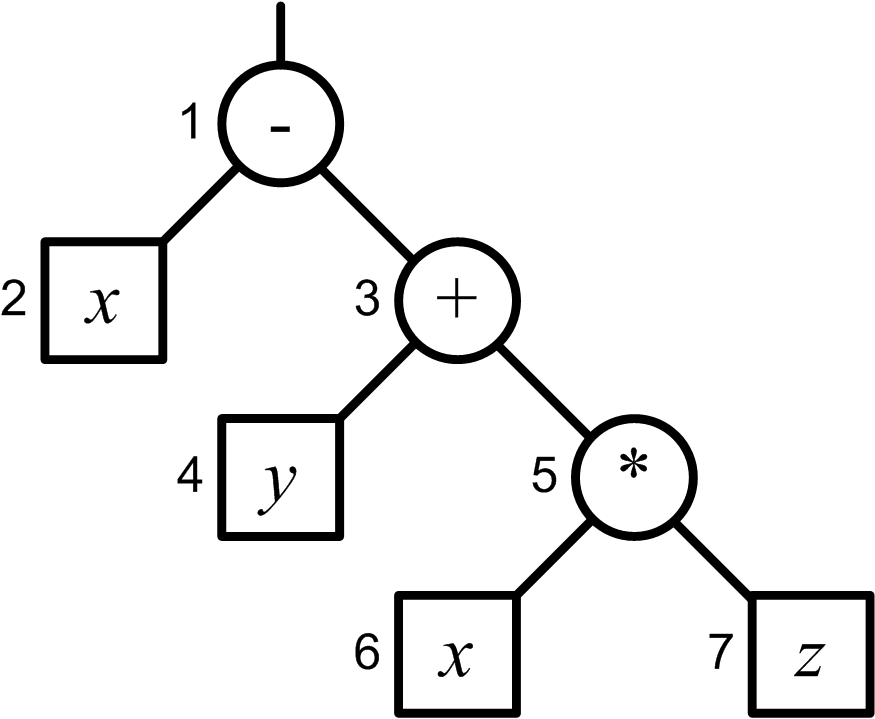
\includegraphics[width=0.3\textwidth]{fig/treeRepParent.png}}
        }
    \end{tabular}
    \caption{Табличное преставление с помощью ссылок на родительский узел}
    \label{fig:rec:treeRepParent}
\end{figure}

При этом для поиска корня дерева можно использовать запрос
\begin{verbatim}
select * from tree where id=pid;
\end{verbatim}

Поиск всех дочерних узлов для узла с известным идентификатором \verb"ID" организуется также весьма просто:
\begin{verbatim}
select * from tree where pid=:ID;
\end{verbatim}

Найти предка, если известен параметр \verb"PID" потомка также весьма просто:
\begin{verbatim}
select * from tree where pid=:PID;
\end{verbatim}

Но вот определить все узлы поддеревьев некоторого узла можно только рекурсивно. Эту проблему решает представление с помощью \emph{вложенных множеств}. Проведя уже знакомую модификацию псевдокода \ref{alg:rec:postfix} легко получим для дерева списочное представление в постфиксной записи. При этом для каждой скобки верхним индексом поставим её вложенность, а нижним --- её номер по порядку:
\[
    \Big(_0^1
        \Big(_1^2 x\Big)_2^2\ 
        \Big(_3^2
            \Big(_4^3 y\Big)_5^3\ 
            \Big(_6^3
                \Big(_7^4 x\Big)_8^4\ 
                \Big(_9^4 z\Big)_{10}^4 *
            \Big)_{11}^3 +
        \Big)_{12}^2 -
    \Big)_{13}^1.
\]

В соответствующей таблице (см. рис. \ref{fig:rec:treeRepNested}) следует определить поля:
\begin{itemize}
    \item значение узла (text);
    \item уровень вложенности (верхний индекс скобок) узла (lvl);
    \item номер (нижний индекс) открывающей скобки узла (l);
    \item номер (верхний индекс) закрывающей скобки узла (r).
\end{itemize}

\begin{figure}
    \centering
    \begin{tabular}{cc}
        \begin{tabular}{|c|c|c|c|}
            \hline\hline
            text&lvl    &l      &r \\
            \hline\hline
            +   &2      &3      &12 \\ \hline
            -   &1      &0      &13 \\ \hline
            *   &3      &6      &11 \\ \hline
            x   &2      &1      &2  \\ \hline
            x   &4      &7      &8  \\ \hline
            y   &3      &4      &5  \\ \hline
            z   &4      &9      &10 \\ \hline
        \end{tabular}
        &\raisebox{-.5\height}{\fbox{
            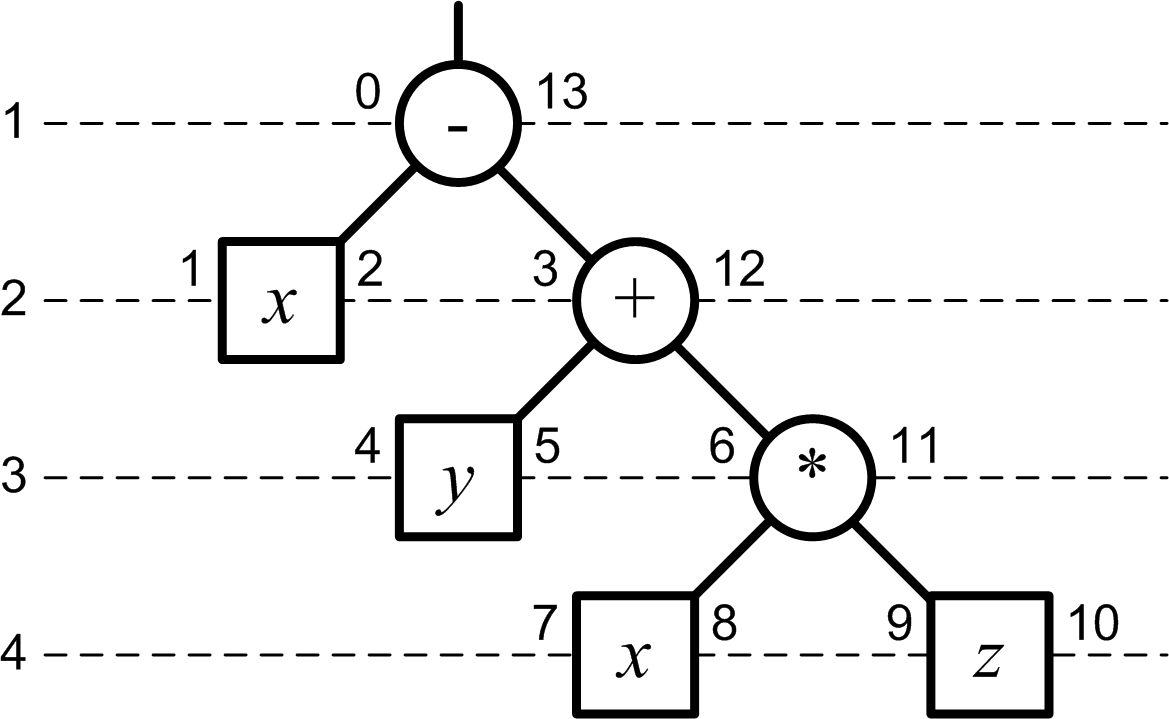
\includegraphics[width=0.4\textwidth]{fig/treeRepNested.png}
        }}
    \end{tabular}
    \caption{Табличное преставление с помощью вложенных множеств}
    \label{fig:rec:treeRepNested}
\end{figure}

Теперь, если известны параметры \verb"LVL", \verb"L", \verb"R" узла то запрос на получение непосредственных потомков будет выглядеть так:
\begin{verbatim}
select * from tree where lvl=:LVL+1 and l>:L and r<:R;
\end{verbatim}

Найти предка можно запросом
\begin{verbatim}
select * from tree where lvl=:LVL-1 and l<:L and r>:R;
\end{verbatim}

Для того, чтобы выбрать все узлы поддеревьев узла достаточно снять ограничение на уровень вложенности:
\begin{verbatim}
select * from tree where l>:L and r<:R;
\end{verbatim}

Приведенные выше способы не накладывают ограничений на глубину дерева. В ряде случаев максимальная глубина дерева известна. Тогда можно воспользоваться следующим рекурсивным способом индексирования вершин дерева.
\begin{enumerate}
    \item База. Корень дерева получает индекс $1$.
    \item Рекурсивный переход. Для всех узлов-потомков $a_1,\ldots,a_n$ некоторого узла с индексом $i$ соответствующие индексы будут $i.1,\ldots,i.n$.
\end{enumerate}

В таблице, кроме поля значения узла (text), отводится соответствующее количество полей (i1,i2,\ldots) для индексов каждого уровня (см. рис. \ref{fig:rec:treeRepConstLevel}).

\begin{figure}
    \centering
    \begin{tabular}{cc}
        \begin{tabular}{|c|c|c|c|c|c|}
            \hline\hline
            text    &i1     &i2     &i3     &i4     &i5 \\
            \hline\hline
            -       &1      &0      &0      &0      &0 \\ \hline
            *       &1      &2      &2      &0      &0 \\ \hline
            +       &1      &2      &0      &0      &0 \\ \hline
            x       &1      &1      &0      &0      &0 \\ \hline
            x       &1      &2      &2      &1      &0 \\ \hline
            y       &1      &2      &1      &0      &0 \\ \hline
            z       &1      &2      &2      &2      &0 \\ \hline
        \end{tabular}
        &\raisebox{-.5\height}{\fbox{
            \includegraphics[width=0.35\textwidth]{fig/treeRepConstLevel.png}
        }}
    \end{tabular}
    \caption{Табличное преставление индексов узлов}
    \label{fig:rec:treeRepConstLevel}
\end{figure}

Запрос всех непосредственных потомков узла с индексом, например, <<1.2>> будет таким
\begin{verbatim}
select * from tree where i1=1 and i2=2 and i3<>0 and i4=0;
\end{verbatim}

Все узлы поддеревьев можно найти запросом
\begin{verbatim}
select * from tree where i1=1 and i2=2 and i3<>0;
\end{verbatim}

Запрос предка узла с индексом, например, <<1.2.2>> будет таким
\begin{verbatim}
select * from tree where i1=1 and i2=2 and i3=0;
\end{verbatim}

Каждый способ табличного представления деревьев имеет свои достоинства и недостатки, которые особенно остро проявляются в случае, если требуется модифицировать дерево.


\section{Рекурсивные алгоритмы}

Рекурсивный алгоритм бинарного поиска приведен в псевдокоде \ref{alg:rec:binSearchRec}. Суть алгоритма в том, что текущий диапазон массива $a[l:r]$ делится пополам. Если элемент в середине этого диапазона $a[m]$ не является искомым, то поиск продолжается либо в левой половине диапазона $a[l:m-1]$, либо в правой $a[m+1:r]$, в зависимости от результата сравнения $a[m]$ с искомым $x$.

Бинарный поиск можно выполнить итеративно (см. псевдокод \ref{alg:rec:binSearchIter}).

\begin{algorithm}
    \caption{binarySearch($a$, $x$, $l$, $r$) --- рекурсивный алгоритм бинарного поиска}
    \label{alg:rec:binSearchRec}
    \begin{algorithmic}[1]
        \REQUIRE{$a$ --- отсортированный по возрастанию массив элементов линейно упорядоченного множества. Длина массива $n$, обращение к элементу по $i$-му индексу: $a[i]$. Первый элемент массива $a[0]$, последний $a[n-1]$. Если $i\geq j$, то $a[i]\geq a[j]$. $l$ --- индекс левой границы, $r$ --- индекс правой границы. $x$ --- искомый элемент. Первый вызов: binarySearch($a$, $x$, $0$, $n-1$)}
        \ENSURE{Индекс найденного элемента. Если элемент не найден, возвращается индекс, равный $-1$.}

        \IF{$l>r$}
            \RETURN{$-1$}
        \ELSE
            \STATE{$m\gets \lfloor\frac{l+r}{2}\rfloor$} 
            \COMMENT{индекс середины диапазона $a[l:r]$}
            \IF{$x=a[m]$}
                \RETURN{$m$}
            \ELSE
                \IF{$x<a[m]$}
                    \RETURN{binarySearch($a$, $x$, $l$, $m-1$)}
                    \COMMENT{поиск в левой половине}
                \ELSE
                    \RETURN{binarySearch($a$, $x$, $m+1$, $r$)}
                    \COMMENT{поиск в правой половине}
                \ENDIF
            \ENDIF
        \ENDIF

    \end{algorithmic}
\end{algorithm}

\begin{algorithm}
    \caption{binarySearch($a$, $x$, $l$, $r$) --- итеративный алгоритм бинарного поиска}
    \label{alg:rec:binSearchIter}
    \begin{algorithmic}[1]
        \WHILE{$l\leq r$}
            \STATE{$m\gets \lfloor\frac{l+r}{2}\rfloor$} 
            \IF{$x=a[m]$}
                \RETURN{$m$}
            \ELSE
                \IF{$x<a[m]$}
                    \STATE{$r\gets m-1$} 
                \ELSE
                    \STATE{$l\gets m+1$} 
                \ENDIF
            \ENDIF
        \ENDWHILE
        \RETURN{$-1$}
    \end{algorithmic}
\end{algorithm}

На практике всегда, когда есть выбор между эквивалентными рекурсивной и итеративной версиями, выбирают версию итеративную. Рекурсивный алгоритм всегда можно свести к итеративному. В худшем случае этот итеративный алгоритм будет использовать стек, и тогда от красоты и наглядности рекурсивного решения не останется ничего. В этом случае, пожалуй стоит подумать над тем, чтобы использовать именно рекурсивное решение.

Пример с бинарным поиском весьма неудачен, потому что он не иллюстрирует основную стратегию рекурсии: \emph{разделяй и властвуй}! Да, пространство поиска разделялось на две части, но властвовали мы только над одной из них. Более удачный пример --- \emph{сортировка слиянием}. Если два массива упорядочены, то объединить их в один массив достаточно просто (см. псевдокод \ref{alg:rec:split}). Суть сортировки слиянием в том, что исходный неотсортированный массив разбивается на две части, которые рекурсивно сортируются по отдельности и затем эти части сливаются в один отсортированный массив (см. псевдокод \ref{alg:rec:splitSort}).

\begin{algorithm}
    \caption{split($a$, $l$, $m$, $r$) --- алгоритм слияния двух упорядоченных по возрастанию массивов}
    \label{alg:rec:split}
    \begin{algorithmic}[1]
    
        \REQUIRE{$a$ --- массив, содержащий две упорядоченные по возрастанию части $a[l:m-1]$ и $a[m:r]$}
        \ENSURE{Часть массива $a[l:r]$, элементы которой упорядочены по возрастанию}
    
        \WHILE{$l<m$ \AND $m\leq r$}
            \IF{$a[l]\leq a[m]$}
                \STATE{$l\gets l+1$} 
            \ELSE
                \STATE{$t\gets a[m]$} 
                \FOR{$i=m-1$ to $l$}
                    \STATE{$a[i+1]\gets a[i]$} 
                \ENDFOR
                \STATE{$a[l]\gets t$} 
                \STATE{$l\gets l+1$} 
                \STATE{$m\gets m+1$} 
            \ENDIF
        \ENDWHILE
    \end{algorithmic}
\end{algorithm}

\begin{algorithm}
    \caption{splitSort($a$, $l$, $r$) --- сортировка слиянием}
    \label{alg:rec:splitSort}
    \begin{algorithmic}[1]
    
        \REQUIRE{$a$ --- массив, элементы $a[l:r]$ которого нужно упорядочить по возрастанию. Первый элемент массива $a[0]$, последний $a[n-1]$. Первый вызов: splitSort($a$, $0$, $n-1$)}
        \ENSURE{Массив $a$, элементы которого упорядочены по возрастанию}
    
        \IF{$l<r$}
            \STATE{$m\gets \lfloor\frac{l+r}{2}\rfloor$} \COMMENT{разделяем}
            \STATE{splitSort($a$, $l$, $m$)} \COMMENT{властвуем}
            \STATE{splitSort($a$, $m+1$, $r$)} \COMMENT{властвуем}
            \STATE{split($a$, $l$, $m+1$, $r$)} \COMMENT{объединяем решения}
        \ENDIF
    \end{algorithmic}
\end{algorithm}

Ход сортировки массива процедурой splitSorn представлен на рисунке \ref{fig:rec:splitSortEx}.
\begin{figure}
\[
\resizebox{\textwidth}{!}
{
    {\xymatrix{
        *{}
            &*{}
                &*{}
                    &*{}
                        &*{}
                            &*{}
                                &*{}
                                    &*{\fbox{4\,1\,9\,5\,2\,6\,8\,3}}\ar@{-}[dllll]\ar@{-}[drrrr]
                                        &*{}
                                            &*{}
                                                &*{}
                                                    &*{}
                                                        &*{}
                                                            &*{}
                                                                &*{}
                                                                    \\
        *{}
            &*{}
                &*{}
                    &*{\fbox{4\,1\,9\,5}}\ar@{-}[dll]\ar@{-}[drr]
                        &*{}
                            &*{}
                                &*{}
                                    &*{}
                                        &*{}
                                            &*{}
                                                &*{}
                                                    &*{\fbox{2\,6\,8\,3}}\ar@{-}[dll]\ar@{-}[drr]
                                                        &*{}
                                                            &*{}
                                                                &*{}
                                                                    \\
        *{}
            &*{\fbox{4\,1}}\ar@{-}[dl]\ar@{-}[dr]
                &*{}
                    &*{}
                        &*{}
                            &*{\fbox{9\,5}}\ar@{-}[dl]\ar@{-}[dr]
                                &*{}
                                    &*{}
                                        &*{}
                                            &*{\fbox{2\,6}}\ar@{-}[dl]\ar@{-}[dr]
                                                &*{}
                                                    &*{}
                                                        &*{}
                                                            &*{\fbox{8\,3}}\ar@{-}[dl]\ar@{-}[dr]
                                                                &*{}
                                                                    \\
        *{\fbox{4}}\ar@{-}[dr]
            &*{}
                &*{\fbox{1}}\ar@{-}[dl]
                    &*{}
                        &*{\fbox{9}}\ar@{-}[dr]
                            &*{}
                                &*{\fbox{5}}\ar@{-}[dl]
                                    &*{}
                                        &*{\fbox{2}}\ar@{-}[dr]
                                            &*{}
                                                &*{\fbox{6}}\ar@{-}[dl]
                                                    &*{}
                                                        &*{\fbox{8}}\ar@{-}[dr]
                                                            &*{}
                                                                &*{\fbox{3}}\ar@{-}[dl]
                                                                    \\
        *{}
            &*{\fbox{1\,4}}\ar@{-}[drr]
                &*{}
                    &*{}
                        &*{}
                            &*{\fbox{5\,9}}\ar@{-}[dll]
                                &*{}
                                    &*{}
                                        &*{}
                                            &*{\fbox{2\,6}}\ar@{-}[drr]
                                                &*{}
                                                    &*{}
                                                        &*{}
                                                            &*{\fbox{3\,8}}\ar@{-}[dll]
                                                                &*{}
                                                                    \\
        *{}
            &*{}
                &*{}
                    &*{\fbox{1\,4\,5\,9}}\ar@{-}[drrrr]
                        &*{}
                            &*{}
                                &*{}
                                    &*{}
                                        &*{}
                                            &*{}
                                                &*{}
                                                    &*{\fbox{2\,3\,6\,8}}\ar@{-}[dllll]
                                                        &*{}
                                                            &*{}
                                                                &*{}
                                                                    \\
        *{}
            &*{}
                &*{}
                    &*{}
                        &*{}
                            &*{}
                                &*{}
                                    &*{\fbox{1\,2\,3\,4\,5\,6\,8\,9}}
                                        &*{}
                                            &*{}
                                                &*{}
                                                    &*{}
                                                        &*{}
                                                            &*{}
                                                                &*{}
    }}
}
\]
    \caption{Пример выполнения splitSort([4,1,9,5,2,6,8,3],0,7)}
    \label{fig:rec:splitSortEx}
\end{figure}

За знаниями по основным алгоритмам можно обратится к книгам \cite{bib:wirth:alghorithms,bib:kernigan:practice}. Нельзя не сказать о фундаментальном труде Дональда Кнута \cite{bib:knuth:artOfProgramming1, bib:knuth:artOfProgramming2, bib:knuth:artOfProgramming3}. Алгоритмы с точки зрения их анализа рассматриваются в книгах \cite{bib:mcconnel:alghorithmAnalysis, bib:miller:secParAlghorithm}.


\section*{Задания}
\addcontentsline{toc}{section}{Задания}

\begin{enumerate}
    \item Доказать по индукции, что  
    \begin{enumerate}
        \item $n!>n^2$ при $n\geq 4$.
        \item $2^n>n^3$ при $n\geq 10$.
        \item $3$ делит $n^3+2n$ при $n>0$.
        \item $6$ делит $n^3-n$ при $n>0$.
        \item $\frac{1}{1\cdot 2}+\frac{1}{2\cdot 3}+\cdots+\frac{1}{n(n+1)}=\frac{n}{n+1}$ при $n\geq 1$.
        \item Формулы \eqref{eq:rec:rec1type} и \eqref{eq:rec:rec1typeSum} эквивалентны.
    \end{enumerate}

    \item Найти решение реккурентности 
    \[
        f(n)=
        \begin{cases}
            c,                  &n=0,\\
            a\cdot f(n-1) + b,  &n\geq 1
        \end{cases}
    \]
    в аналитическом виде.
    
    \item Алгоритм поиска $\text{НОД}$ --- наибольшего общего делителя (gcd\footnote{gcd --- greatest common divisor}) рекурсивно задается так:
    \[
        \text{НОД}(a,b)=
        \begin{cases}
            b,                      &a=0\\
            \text{НОД}(b \bmod a,a),&a>0
        \end{cases}
    \]
    Найдите $\text{НОД}(210,119)$
    
    \item Понятие упорядоченного набора элементов, т.е. кортежа $(a_1,a_2,\ldots,a_n)$ длины $n$ можно свести рекурсивно к понятию \emph{упорядоченной пары} (tuple):
    \[
        (a_1,\ldots,a_n)=
        \begin{cases}
            ()=\emptyset, &n=0,\\
            (a_1,a_2,\ldots,a_n)=(a_1,(a_2,\ldots,a_n)), &n>0.
        \end{cases}
    \]
    Так, например 
    \begin{itemize}
        \item $()=\emptyset$; 
        \item $(a_1)=(a_1,())=(a_1,\emptyset)$;
        \item $(a_1,a_2)=(a_1,(a_2,\emptyset))$;
        \item $(a_1,a_2,a_3)=(a_1,(a_2,(a_3,\emptyset)))$.
    \end{itemize}
    
    То есть, определяя кортеж длины $n$ можно обойтись лишь понятием упорядоченной пары. Для упорядоченной пары $(a,b)$, в отличие от множества $\{a,b\}$, характерно $(a,b)\neq(b,a)$, если $a\neq b$. Упорядоченную пару можно определить через множества\footnote{Казимир Куратовский, 1921}: $(a,b)=\{\{a\},\{a,b\}\}$. Это, в частности, означает что понятие кортежа лишь искусственный конструкт, созданный на основе множеств исключительно для удобства. Тогда, объединяя вышеизложенное, можно определить кортеж длины $n$ так:
    \[
        (a_1,\ldots,a_n)=
        \begin{cases}
            ()=\emptyset, &n=0,\\
            (a_1,a_2,\ldots,a_n)=\{\{a_1\},\{a_1, (a_2,\ldots,a_n)\}\}, &n>0.
        \end{cases}
    \]
    
    Тогда:
    \begin{itemize}
        \item $()=\emptyset$; 
        \item $(a_1)=\{\{a_1\},\{a_1,()\}\}=\{\{a_1\},\{a_1,\emptyset\}\}$;
        \item $(a_1,a_2)=\{\{a_1\},\{a_1,(a_2)\}\}=\{\{a_1\},\{a_1,\{\{a_2\},\{a_2,\emptyset\}\}\}\}$.        
    \end{itemize}

    Задание
    \begin{enumerate}
        \item Найти представление множеством кортежа $(a_1,a_2,a_3)$;
        \item Написать программу для нахождения представления произвольного кортежа множеством;
        \item Определить, какому кортежу соответствует $\{\{\emptyset\}\}$;
        \item Определить, какому кортежу соответствует 
        \begin{enumerate}
            \item $\{\{b,\{\{a,\emptyset\},\{a\}\}\},\{b\}\}$;
            \item $\{\{a,\{\{c,\{\{b,\emptyset\},\{b\}\}\},\{c\}\}\},\{a\}\}$;
            \item $\{\{d,\{\{a,\{\{c,\{\{b,\emptyset\},\{b\}\}\},\{c\}\}\},\{a\}\}\},\{d\}\}$.
        \end{enumerate} 
        \item Написать программу для нахождения кортежа по представлению множеством, с учетом того, что $\{a,b\}=\{b,a\}$. Значениями координат кортежа могут быть лишь одиночные символы. Пустое множество значением координаты быть не может.
    \end{enumerate}
    
    \item Решить задачу разрезания торта: сколько кусков торта можно получить, делая $n$ прямолинейных разрезов ножом. Усложните задачу, предполагая, что торт разрезается двумя прямолинейными резами, исходящими из одной точки.
    
    \item Построить дерево, постфиксную и префиксную запись выражения в инфиксной форме:
    \begin{enumerate}
        \item $(a+b/c)*(d-e*f)$;
        \item $(a+b-c)*(d+e)*f$;
        \item $(a+b-c)*(d+e)-f$;
        \item $(a+b/c)-(d-e)*f$;
        \item $(a+b)/c-d/e*f$;
        \item $(a+b)/(c-(d-e)*f)$.
    \end{enumerate}
    
    \item Преобразовать в инфиксную форму выражения в постфиксной форме:
    \begin{enumerate}
        \item $abc+d*-$;
        \item $ab+c-d*$;
        \item $ab*cd+e-+$;
        \item $ab+cde-+*$;
        \item $abc-*de+-$;
        \item $abc/*de+-$.
    \end{enumerate}

    \item Представить дерево в табличном виде с помощью вложенных множеств, соответствующее формуле:
    \begin{enumerate}
        \item $(a+b/c)*(d-e*f)$;
        \item $(a+b-c)*(d+e)*f$;
        \item $(a+b-c)*(d+e)-f$;
        \item $(a+b/c)-(d-e)*f$;
        \item $(a+b)/c-d/e*f$;
        \item $(a+b)/(c-(d-e)*f)$.
    \end{enumerate}

    \item Напишите псевдокод для вычисления $n$-го числа Фибоначчи рекурсивно и итеративно. Оцените какой алгоритм будет работать быстрее.
\end{enumerate}
 %Рекурсия
    \chapter{Анализ алгоритмов}
\label{ch:alg}

Согласно \cite{bib:knuth:artOfProgramming1} \emph{алгоритмом} называют набор конечного числа правил, задающих последовательность выполнения операций для решения задачи определённого типа, имеющий пять особенностей.
\begin{enumerate}
    \item \emph{Конечность}. Алгоритм всегда должен заканчиваться после конечного числа шагов. \emph{Метод вычислений}, в отличие от алгоритма, не обладает свойством конечности.
    
    \item \emph{Определенность}. Каждый шаг алгоритма должен быть четко определен. Языки программирования, например, четко определяют значение (смысл) каждого предложения. Метод вычислений, выраженный на языке программирования, называется \emph{программой}.
    
    \item \emph{Ввод}. Алгоритм имеет определенное (иногда нулевое) число входных данных.
    
    \item \emph{Вывод}. Алгоритм имеет определенное число выходных данных.
    
    \item \emph{Эффективность}. Алгоритм эффективен, когда все его шаги достаточно просты для того, чтобы их можно было точно выполнить в течение конечного промежутка времени.
\end{enumerate}

Анализу подвергаются следующие характеристики:
\begin{itemize}
    \item время выполнения алгоритма;
    \item объем памяти, необходимый для выполнения алгоритма.
\end{itemize}

Следует заметить: то, что названо <<временем выполнения алгоритма>> вовсе не измеряется в секундах. Оценка в секундах будет характеризовать скорее конкретный компьютер, исполняющий алгоритм, а не сам алгоритм. Поэтому термин <<время>> в данном контексте следует понимаеть скорее как <<число шагов>>\footnote{А число шагов, очевидно, отразится и на времени исполнения каким бы то ни было компьютером}. Впрочем, и точное количество шагов при анализе не представляет большого интереса. Достаточно приближенно оценить зависимость количества шагов (операций) от размера входных данных.

Далее внимание уделяется именно анализу <<времени>> выполнения алгоритма, а не затрат памяти. Впрочем, подход остается тем же. 

Подробнее об анализе алгоритмов см. \cite{bib:haggard:discrmathprogrammer}. Книги \cite{bib:miller:secParAlghorithm, bib:mcconnel:alghorithmAnalysis} целиком посвящены теме анализа алгоритмов.


\section{Скорости роста}

Одну и ту же задачу можно решить разными алгоритмами. Более того, один и тот же алгоритм можно выразить разными программами на различных языках программирования. Одна и та же программа может быть выполнена отличающимися по производительности компьютерами.

С практической точки зрения важно сделать обоснованный выбор лучшего из алгоритмов, решающих одну и ту же задачу, основываясь на изучении самого алгоритма, а не выражая алгоритм в программе (и тем более не проводя тестовых запусков на компьютере). Это основная задача анализа. 

При этом точные значения характеристик (время, память) не столь важны. Важнее дать приближенную оценку \emph{скорости} их роста с увеличением размера входных данных $n$. То есть интерес представляет общий характер поведения алгоритма, а не его подробности.

Допустим, что для алгоритма $A$ можно вывести функцию $g:\mathbb{N}\to[0,\infty)$, которая по заданному размеру данных $n$ вычисляет время выполнения алгоритма (или затраты памяти). При этом данную функцию можно отнести к следующим трем классам скорости роста функций:
\begin{enumerate}
    \item Класс функций, растущих по крайней мере так же быстро как $f(n)$. Обозначается этот класс как $\Omega(f(n))$ (читается как \emph{омега большое}). Функция $g(n)$ принадлежит этому классу(обозначается $g\in\Omega(f)$), если при всех значениях аргумента $n$, больших некоторого порогового значения $n_0$, значение $g(n)>c\cdot f(n)$ для некоторого положительного числа $c$.
    
    \item Класс функций, растущих не быстрее $f(n)$. Обозначается этот класс как $O(f(n))$ (читается как \emph{о большое}). Функция $g(n)$ принадлежит этому классу (обозначается $g\in O(f)$), если при всех значениях аргумента $n$, больших некоторого порогового значения $n_0$, значение $g(n)\leq c\cdot f(n)$ для некоторого положительного числа $c$.
    
    \item Класс функций, растущих той же скоростью, что и $f(n)$. Обозначается этот класс как $\Theta(f(n))$ (читается как \emph{тета большое}). Формально $\Theta(f(n))=\Omega(f(n))\cap O(f(n))$.
\end{enumerate}

Таким образом при анализе алгоритмов не столь важно \emph{точно} вывести функцию $g$, сколь определить какому классу скорости роста она принадлежит. Из перечисленных классов для анализа наиболее важен класс $O(f)$. Проверить, принадлежит ли функция классу $O(f)$ можно двумя способами: с помощью данного выше определения класса $O(f)$, либо воспользовавшись следующим описанием:
\[
    g\in O(f),\text{если} \lim_{n\to\infty}\frac{g(n)}{f(n)}=c
\]
для некоторой константы $c$. Иными словами, если удается найти предел отношения $g(n)/f(n)$ и он меньше бесконечности, то $g\in O(f)$. Если предел найти сложно, то по правилу Лопиталя можно заменить предел отношения функций пределом отношения их производных.

$O(f)$ является классом эквивалентности $f$ и для некоторой функции $g$ правильно писать $g\in O(f)$, но иногда по соглашению пишут $g=O(f)$, что на самом деле означает именно $g\in O(f)$.

Скорость роста некоторых функций $f$ проиллюстрирована в таблице \ref{alg:tbl:gorwth}. Так, например, если обработка на компьютере массива входных данных размером $n=1$ алгоритмом с $g(n)=n^2$ составляет $10^{-9}$ секунд(наносекунду), то обработка массива из $100$ элементов займет $10^{-3}$ секунд. Но если для обработки массива используется алгоритм $g(n)=2^n$, и массив из одного элемента обрабатывается за $10^{-9}$ с., то $100$ элементный массив будет обработан приблизительно за $20000$ миллиардов лет.
\begin{table}
    \centering
    \begin{tabular}{||r||r|r|r|r|r|r|}
        \hline\hline
        $n$ & $\log_2n$ & $n$ & $n\log_2n$ & $n^2$ & $n^3$ & $2^n$\\ \hline\hline
          1 & 0.00 &   1 &    0.00 &     1 &       1 &                                 2\\
          2 & 1.00 &   2 &    2.00 &     4 &       8 &                                 4\\
          4 & 2.00 &   4 &    8.00 &    16 &      64 &                                16\\
          5 & 2.32 &   5 &   11.61 &    25 &     125 &                                32\\
         10 & 3.32 &  10 &   33.22 &   100 &    1000 &                              1024\\
         20 & 4.32 &  20 &   86.44 &   400 &    8000 &                           1048576\\
         40 & 5.32 &  40 &  212.88 &  1600 &   64000 &                     1099511627776\\
         60 & 5.91 &  60 &  354.41 &  3600 &  216000 &               1152921504606846976\\
         80 & 6.32 &  80 &  505.75 &  6400 &  512000 &         1208925819614629174706176\\
        100 & 6.64 & 100 &  664.39 & 10000 & 1000000 &   1267650600228229401496703205376\\
        \hline
    \end{tabular} 
    \caption{Скорость роста функций}
    \label{alg:tbl:gorwth}
\end{table}

Важными классами роста являются классы, образуемые \emph{полиномиальными} функциями 
\begin{equation}
    P(n)=a_k\cdot n^k + a_{k-1}\cdot n^{k-1} + \cdots + a_1\cdot n + a_0,
    \label{eq:alg:polinom}
\end{equation}
где $a_k\neq 0$. Считается, например, что если у алгоритма полиномиальное время работы, то удастся создать компьютер, выполняющий алгоритм за приемлемое время для больших $n$, а если время работы алгоритма растет быстрее чем любой полином\footnote{Например, $g(n)\in O(2^n)$}, то надежды на это нет\footnote{Это может изменится с приходом эры квантовых компьютеров}.

Быстрорастущие функции доминируют над функциями с более медленным ростом. Поэтому, если $g(n)$ представляет собой сумму двух или нескольких таких функций, то часто отбрасываются все функции, кроме тех, которые растут быстрее всего. Также, если функция $g(n)=c\cdot f(n)$, то можно отбросить $c$: $g\in O(f)$. Например для полиномов (см. формулу \eqref{eq:alg:polinom}) справедливо $P(n)\in O(n^k)$.

Некоторые функции $f$, упорядоченные по возрастанию скорости:$f(n)=1$, $f(n)=\log_2n$, $f(n)=n$, $f(n)=n\log_2n$, $f(n)=n^2$, $f(n)=n^2\log_2n$, $f(n)=n^3$, \ldots, $f(n)=n^k$, \ldots, $f(n)=2^n$, $f(n)=n!$, $f(n)=n^n$, \ldots.

\begin{exampl} 
    \label{exampl:alg:strongest}
    Функция $g(n)=5n^3+2\log_2n$ принадлежит классу $O(n^3)$.\qed
\end{exampl}

Далее будут рассмотрены несколько методик оценки сложности, которые позволяют вывести $g(n)$ для алгоритма.


\section{Классы входных данных}

Зафиксировав размер входных даннных $n$, можно тем не менее видеть, что в большинстве случаев время выполнения алгоритма для различных наборов данных одного размера также будет различным. Действительно, алгоритмы редко бывают линейными, чаще они содержат операции \emph{выбора}, выполняющие различные действия в зависимости от условий, меняющихся в ходе выполнения.

\begin{exampl}
    Необходимо найти индекс первого элемента в неотсортированном массиве длины $n$, равного искомому.
\end{exampl}
\begin{proof}
    В лучшем случае искомый элемент будет в самом начале массива (первым) и потребуется только одна операция сравнения. Лучший случай имеет сложность $O(1)$. В худшем случае искомого значения в массиве не будет, и придется выполнить $n$ сравнений. Сложность худшего случая $O(n)$. В случае, если значение искомого элемента находится в $i$-й ячейке массива, то потребуется $i$ сравнений. Оценить, сколько операций сравнения будет в среднем, можно, приняв некоторые допущения (которые иногда могут оказаться не вполне справедливыми):
    \begin{enumerate}
        \item искомый элемент может оказаться в любом месте массива с равной вероятностью $p_i=\frac{1}{n}$;
        \item искомого элемента может не оказаться в массиве в половине случаев.
    \end{enumerate}

    Тогда, среднее количество операций сравнений может быть найдено как
    \[
        g(n)=\frac{1}{2}n+\frac{1}{2}\sum_{i=1}^{n}p_i\cdot i=\frac{1}{2}\left(n+\frac{1}{n}\frac{n(n+1)}{2}\right)=
        \frac{3}{4}n+\frac{1}{4}.
    \]

    Сложность среднего случая $g\in O(n)$.
\end{proof}

Оценку лучшего случая проводят редко --- он не представляет большого интереса. Оценка наихудшего случая дает верхнюю оценку времени работы. Обычно дают оценку именно худщего случая. Оценить средний случай сложнее всего, но именно эта оценка наиболее адекватна. Общий подход оценки среднего случая заключается в следующем. Все возможные варианты входных наборов данных длины $n$ разбивается на группы. Время работы алгоритма на всех входных наборах группы должно быть одинаковым. Определяется вероятность с которой некоторый входной набор принадлежит каждой группе. Среднее время работы вычисляется по формуле
\[
    g(n)=\sum_{i=1}^{m}p_i\cdot t_i,
\]
где $n$ --- размер входных данных, $m$ --- число групп, $p_i$ --- вероятность принадлежности входного набора $i$-й группе, $t_i$ --- время работы алгоритма для $i$-й группы. Иногда предполагают равную вероятность попадания в любую группу и тогда 
\[
    g(n)=\frac{1}{m}\sum_{i=1}^{m}t_i.
\]

В рассмотренном примере при оценке среднего случая все множество входных наборов данных было разбито на два подмножества: содержащие искомый элемент и не содержащие. Множество наборов, содержащих искомый элемент, было разбито на $n$ групп: в $i$-й группе искомый элемент находится в $i$-й ячейке.


\section{Анализ программ}

Одна и та же задача может быть решена различными алгоритмами, выраженными в различных программах. Например, задача поиска максимального элемента среди трех может быть решена, например, псевдокодом \ref{alg:alg:maxOfThree1} или \ref{alg:alg:maxOfThree2}. Первый вариант содержит меньше условных конструкций, испльзует больше памяти и его проще понять. Тем не менее в ходе выполнения приведенных программ выполняется по два сравнения и с этой точки зрения у них одинаковый уровень сложности. Алгоритмы решения некоторых задач принадлежат разным классам скоростей роста времени выполнения.

\begin{algorithm}
    \caption{Поиск наибольшенго элемента среди $a,b,c$}
    \label{alg:alg:maxOfThree1}
    \begin{algorithmic}[1]
        \REQUIRE{$a,b,c$ --- три значения, среди которых ищется наибольший}
        \ENSURE{наибольший элемент}

        \STATE{$m\gets a$} 
        \IF{$b>m$}
            \STATE{$m\gets b$}
        \ENDIF
        \IF{$c>m$}
            \STATE{$m\gets c$}
        \ENDIF
        \RETURN{$m$}
    \end{algorithmic}
\end{algorithm}
\begin{algorithm}
    \caption{Поиск наибольшенго элемента среди $a,b,c$}
    \label{alg:alg:maxOfThree2}
    \begin{algorithmic}[1]
        \REQUIRE{$a,b,c$ --- три значения, среди которых ищется наибольший}
        \ENSURE{наибольший элемент}

        \IF{$a>b$}
            \IF{$c>a$}
                \RETURN{$c$}
            \ELSE
                \RETURN{$a$}
            \ENDIF
        \ELSE[$b\geq a$]
            \IF{$c>b$}
                \RETURN{$c$}
            \ELSE
                \RETURN{$b$}
            \ENDIF            
        \ENDIF
    \end{algorithmic}
\end{algorithm}

Так или иначе, но алгоритм должен быть <<выражен>>. В программе, в блок схеме, в словесном описании\ldots Далее приводится ряд примеров анализа программ, в которых выражены алгоритмы. Будует использован псевдокод, в котором представлены основные элементы структурного программирования: \emph{последовательность}, \emph{выбор}, \emph{повторение}.

Оценка последовательности наиболее проста (см. псевдокод \ref{alg:alg:sequention}). 
\begin{algorithm}
    \caption{$A(n)$ --- последовательность в структурном программировании}
    \label{alg:alg:sequention}
    \begin{algorithmic}[1]
        \REQUIRE{$S_1,S_2,\ldots,S_k$ --- последовательно выполняющиеся операторы. Для каждого из них известна оценка их времени выполнения: $g_{S_1}(n), g_{S_2}(n),\ldots,g_{S_k}(n)$}
        
        \STATE{$S_1$} 
        \STATE{$S_2$} 
        \STATE{$\ldots$} 
        \STATE{$S_k$} 
    \end{algorithmic}
\end{algorithm}
Очевидно, что оценка алгоритма --- это сумма оценок каждого оператора последовательности:
\[
g_A(n)=\sum_{i=1}^{k} g_{S_i}(n).
\]

Выбор в структурном программировании представлен условным оператором (см. псеводокод \ref{alg:alg:select}).
\begin{algorithm}
    \caption{$A(n)$ --- выбор в структурном программировании}
    \label{alg:alg:select}
    \begin{algorithmic}[1]
        \REQUIRE{$S_1,S_2$ --- операторы с известной оценкой времени выполнения: $g_{S_1}(n), g_{S_2}(n)$. Оценка условия $C$ --- $g_{C}(n)$}
        
        \IF{$C$}
            \RETURN{$S_1$}
        \ELSE
            \RETURN{$S_2$}
        \ENDIF
    \end{algorithmic}
\end{algorithm}
Для оценки лучшего случая выбора, очевидно:
\[g_A(n)=g_C(n)+\min\{g_{S_1}(n), g_{S_2}(n)\}.\]
Худшего случая:
\[g_A(n)=g_C(n)+\max\{g_{S_1}(n), g_{S_2}(n)\}.\]
Среднего случая:
\[g_A(n)=g_C(n) + p_{S_1}\cdot g_{S_1}(n) + p_{S_2}\cdot g_{S_2}(n),\]
где $p_{S_i}$ --- вероятность выбора оператора $S_i$.

После того, как в получившихся формулах будут отброшены медленно растущие слагаемые (см. пример \ref{exampl:alg:strongest}), то оценки для худшего и среднего случая будут совпадать.

Повторение в структурном программировании представлено конструкцией цикла (см. псевдокод \ref{alg:alg:loop}). Анализ цикла прост, когда это цикл с заданным числом повторений. В противном случае оценка количества итераций цикла не столь тривиальна.
\begin{algorithm}
    \caption{$A(n)$ --- повторение в структурном программировании}
    \label{alg:alg:loop}
    \begin{algorithmic}[1]
        \REQUIRE{$S$ --- оператор цикла с известной оценкой времени выполнения $g_S(i)$.}
        
        \FOR{$i=1$ to $n$}
            \STATE{$S$}\COMMENT{время выполнения зависит от $i$}
        \ENDFOR
    \end{algorithmic}
\end{algorithm}
Число ключевых операций цикла в данном случае находится как
\[
    g_A(n)=c+\sum_{i=1}^{n}(c+g_S(i)),
\]
где $c$ --- количество ключевых операций, затрачиваемых на проверку условия окончания цикла (часто $c=0$).

При анализе часто возникают суммы, которые можно свести к замкнутой форме. Далее приводятся наиболее полезные из них. В числе простейших:
\begin{gather}
    \sum_{i=1}^{n}1=n\\
    \sum_{i=1}^{n}c=cn\\
    \sum_{i=1}^{n}i=\frac{n(n+1)}{2}.
\end{gather}
Более сложные суммы:
\begin{gather}
    \sum_{i=1}^{n}i^2=\frac{n(n+1)(2n+1)}{6}\\
    \sum_{i=0}^{n}A^i=\frac{A^{n+1}-1}{A-1}\label{eq:alg:sumsApowi}\\
    \sum_{i=1}^{n}i2^i=(n-1)2^{n+1}+2\\
\end{gather}
Следует обратить внимание на то, что в формуле \eqref{eq:alg:sumsApowi} нижняя граница индекса равна нулю. Важным частным случаем этой формулы является 
\[
    \sum_{i=0}^{n}2^i=2^{n+1}-1.
\] 
Часто используется и биномиальная теорема:
\begin{equation}
    \label{eq:alg:binomTheorem}
    \sum_{i=0}^{n}\binom{n}{i}A^{i}B^{n-i} = (A+B)^{n},
\end{equation}
где $\binom{n}{i}=\frac{n!}{i!(n-i)!}$.
Наконец, несколько приближенных формул:
\begin{gather}
    \sum_{i=1}^{n}\frac{1}{i}\approx \ln n\\
    \sum_{i=1}^{n}\log_2i\approx n\log_2n-1.5
\end{gather}


\section{$P$ и $NP$}

Задачи, оценка сложности которых по времени выполнения не превышает $O(n^k)$ называются \emph{полиномиальными} (см. полином ф-ла \eqref{eq:alg:polinom}). \emph{Точное} решение подобных задач может быть найдено за <<разумный>> промежуток времени. Все подобные задачи относятся к классу $P$ --- классу задач \emph{полиномиальной сложности}. Также такие задачи назваются \emph{практически разрешимыми}.

Для задачи, образующих класс $NP$ --- класс \emph{недетерминированной полиномиальной сложности}, до сих пор не известно детерминированных алгоритмов, способных решать их за <<разумное>> время (т.е. полиномиальных). Детерминированным называется алгоритм, вывод которого полностью определяется его вводом. Иначе, алгоритм называется недетерминированным (например, вывод такого алгоритма зависит не только от ввода, но и от обращений к генератору случайных чисел). Задачи класса $NP$ называются также <<практически наразрешимыми>>. Детерминированные алгоритмы решения таких задач хоть и существуют, но они имеют сложность превышающую $O(2^n)$ (большинство имеют экспоненциальную или факториальную сложность). 

Так как решать $NP$ задачу детерминированным алгоритмом (т.е. алгоритмом сложнее $O(2^n)$) бессмысленно, то на практике, чтобы получить удовлетворительное решение, выполняют некоторое подобие попытки его угадать. Иногда такая попытка успешна (близкое к оптимальному решение получено), иногда нет (тогда попытку можно повторить). Попытка состоит из двух шагов.

\begin{enumerate}
    \item Недетерминированный полиномиальный алгоритм генерирует некоторый вариант решения.
    \item Детерминированный алгоритм проверяет является ли решение правильным.
\end{enumerate}

В целом попытка представляет собой недетерминированный алгоритм полиномиальной сложности. Этим и объясняется название $NP$ класса. Хотя оба шага попытки и полиномиальны, но число попыток может оказаться экспоненциальным или факториальным (т.е. оценка количества попыток превышает $O(2^n)$).

К классу $NP$ относится задача о коммивояжере.
\begin{exampl}[Задача о коммивояжере]
    Задан набор городов и стоимость путешествия между любыми из них. Необходимо определить порядок, в котором следует посетить все города по одному разу и вернуться в исходный город, такой, чтобы общая стоимость путешествия оказалась минимальной.
\end{exampl}
\begin{proof}[Подход к решению]
    Всех возможных обходов $n$ городов, очевидно, $n!$. На данный момент не придумано детерминированного алгоритма, который занимался бы просмотром всех возможных путей. Уже для $20$ городов количество вариантов становится просто чудовищным. Читателю предлагается посчитайть самостоятельно, сколько времени потребуется его компьютеру, чтобы решить данную задачу(можно принять оптимистичное допущение, что за один такт он складывает два числа\ldots).
    
    Данная задача относится к классу $NP$, если мы определим полиномиальные алгоритмы для каждого из вышеизложенных шагов попытки.
    
    Как сгенерировать некоторый обход $n$ городов? Например так: записать названия городов в список городов; случайным образом выбрать город из списка городов, а затем удалить его оттуда, чтобы он не появился второй раз; повторить случайный выбор $n$ раз. Очевидно, что сложность генерации случайного обхода $O(n)$. Так как этот алгоритм недетерминирован, то каждый раз (с большой вероятностью) будет получаться новый порядок.
    
    Проверка стоимости также имеет сложность $O(n)$, так как для этого достаточно просуммировать $n$ стоимостей путешествия.
    
    Оба алгоритма полиномиальны, а поэтому задача о комивояжере принадлежит классу $NP$.
\end{proof}

Важно отметить что задачи класса $P$ также принадлежат и классу $NP$ ($P\subseteq NP$). Например, задача сортировки элементов массива принадлежат классу $P$ (сложность алгоритмов её решения находится между $O(n\log_2n)$ и $O(n^2)$). Но её можно решать также, как $NP$ задачу: генерировать случайную последовательность элементов массива ($O(n)$) и проверять, что она упорядочена ($O(n)$). А вот справедливо ли обратное ($P\supseteq NP$), то есть в нонечном итоге совпадают ли эти классы $P=NP$, до сих пор не доказано\footnote{По крайней мере еще никто не решил задачу коммивояжера полиномиальным детерминированным алгоритмом}.

Выделяют понятие \emph{$NP$-полная} задача. Задача называется $NP$-полной, если к ней можно свести все остальные задачи класса $NP$. Задача $A$ сводится (редуцируется) к задаче $B$, если алгоритм решения задачи $A$ можно преобразовать таким образом, чтобы он решал задачу $B$.

\begin{exampl}
    Гамильтоновым циклом в графе называется путь, проходящий через каждую вершину только один раз.
    
    Задача о поиске гамильтонова цикла сводится к задаче о коммивояжере следующим образом. Пусть $n$ --- количество вершин в графе. Каждая вершина графа --- это город. Стоимость пути вдоль каждого ребра графа полагается равной $1$. Стоимость пути между городами полагается равной $2$, если соответствующие вершины графа не соединены ребром.
    
    Теперь, если будет решена задача о коммивояжере, то будет найден кратчайший циклический путь, проходящий единожды по всем городам. Если стоимость найденного пути равна $n$ (то есть он состоит из ребер веса $1$), то этому пути соответствует гамильтонов цикл в графе. Если стоимость путешествия превышает $n$, то гамильтонова цикла в графе нет.
    \qed
\end{exampl}

Есла задача $A$ выполняется за полиномиальное время и сводима к $B$, то и задача $B$ решается за полиномиальное время. Практически применимых $NP$-полных задач очень много и, если хоть для одной из них будет найден полиномиальный детерминированный алгоритм, то все задачи будут им решены. До сих пор ни одна из таких попыток успехом не увенчалась. 

Далее перечислены формулировки некоторых $NP$-полных задач.
\begin{itemize}
    \item Раскраска графа. Вершины графа можно <<раскрасить>> в разные цвета так, чтобы концы каждого ребра были раскрашены разными цветами. Очевидно, что в графе с $n$ вершинами можно раскрасить вершины в $n$ разных цветов. В данной задаче требуется определить минимально необходимое количество цветов для такой раскраски.
    
    \item Раскладка по ящикам. Имеется набор объектов различных размеров $s_1,s_2,\ldots,s_n$. Имеется также некоторое количество ящиков фиксированного размера (самый большой объект в ящик входит). Необходимо определить наименьшее количество ящиков, необходимое для раскладки всех объектов.
    
    \item Упаковка рюкзака. Имеется $n$ объектов объемов $s_1,s_2,\ldots,s_n$ и стоимостей $c_1,c_2,\ldots,c_n$. Требуется упаковать рюкзак объемом $K$, так, чтобы его стоимость была максимальной.
    
    \item Сумма элементов подмножеств. Имеется $n$ объектов весами $s_1,s_2,\ldots,s_n$. Требуется найти такое подмножество объектов, чтобы сумма весов объектов, в него входящих, не превышала верхней границы $K$, но была наиболее близка к ней.
    
    \item Истинность КНФ выражения. КНФ --- последовательность булевых выражений, связанных операторами AND ($\land$), причем каждое выражение есть последовательность булевых переменных или их отрицаний, связанных операторами OR ($\lor$). Например:
    \[
        (a\lor b)\land(\overline{a}\lor c)\land(a\lor b\lor\overline{c}\lor\overline{d}).
    \]
    Существуют ли у переменных, входящих в выражение, такие значения истинности, подстановка которых делает все выражение истинным. Как число переменных $n$, так и сложность выражения не ограничены.
    
    \item Планирование работ. Имеется набор из $n$ работ. Известно время, необходимое для завершения каждой работы $t_1,t_2,\ldots,t_n$. Известны сроки $d_1,d_2,\ldots,d_n$, к которым работы должны быть завершены, а также штрафы $p_1,p_2,\ldots,p_n$, которые будут взысканы при срыве сроков. Необходимо установить последовательность выполнения работ, чтобы свести штрафы к минимуму.
\end{itemize}

В качестве упражнения читателю предлагается провести аналогии между приведенными обобщенными формулировками задач и практическими задачами. 

Следует также отметить, что кроме $NP$ выделют и другие классы сложности, например, $coNP$,$PS$, $ZPP$, $PP$, $RP$ и т.д. Узнать больше об этих классах можно в \cite{bib:hopkroft:automateIntro}.


\section{Вычислимое и невычислимое}

Формальное определение вычислимости довольно сложно и интуитивно. Далее изложены некоторые важные следствия так называемого тезиса Черча-Тьюринга, заключающегося в двух словах в том, что лишь некоторые функции из возможных могут быть вычислены. Два ученых практически одновременно получили результаты, занимаясь исследованиями в этой области в 1930-х годах. Можно сказать, что работа Тьюринга заложила фундамент современной вычислительной техники. Следует предупредить, что тезис Черча-Тьюринга является лишь тезисом, гипотезой --- его (пока?) невозможно ни доказать, ни опровергнуть. 

Как было указано выше, особенностью алгоритма явлеется его эффективность. То есть каждый шаг должен быть прост для выполнения. Прост --- значит, что его, например, может выполнить человек с помощью карандаша и бумаги за небольшое время.

Алан Тьюринг определил абстрактную машину, названную в честь создателя <<машиной Тьюринга>>, каждый шаг работы которой весьма прост. Машина Тьюринга считается эквивалентом понятия метода вычислений (или алгоритма). Также считается (пока мы верим в тезис Черча-Тьюринга), что машина Тьюринга способна делать все то, что доступно современному компьютеру. И если, например, доказано, что машина Тьюринга нечто вычислить не в силах, то и компьютеру это недоступно. 

\begin{figure}[!ht]
    \[
        \begin{array}{cccccccc}
            \cline{2-8}
            \multicolumn{1}{r}{L:}
                &\multicolumn{1}{|c|}{\diamondsuit}
                    &\multicolumn{1}{|c|}{a}
                        &\multicolumn{1}{|c|}{a}
                            &\multicolumn{1}{|c|}{b}
                                &\multicolumn{1}{|c|}{b}
                                    &\multicolumn{1}{|c|}{\diamondsuit}
                                        &\multicolumn{1}{|c}{\cdots}
                                            \\ 
            \cline{2-8}
            &&\Uparrow&&&&&\\
            &&S&&&&&
        \end{array}
    \]
    \caption{Машина Тьюринга}
    \label{fig:alg:turingMachine}
\end{figure}

Машину Тьюринга (см. рис. \ref{fig:alg:turingMachine}) составляют:
\begin{itemize}
    \item блок управления $S$;
    \item бесконечная в одну сторону (вправо) лента ячеек памяти $L$;
    \item головки чтения-записи значений ячеек $\Uparrow$.
\end{itemize}

Блок управления обладает множеством \emph{состояний}, одно из которых является \emph{текущим} и \emph{функцией переходов}. Одно из состояний является \emph{стартовым}: когда машина начинает работу, то это состояние является текущим. Одно или несколько состояний также являются \emph{завершающими} --- перейдя в это состояние, блок управления прекращает работу машины. 

Перед началом работы машины в ячейки ленты записываются символы из множества ленточных символов --- входные данные. Обычно первая (крайняя левая) ячейка ленты остается пустой, входные данные же записываются последовательно слева-направо, начиная со второй ячейки. Среди ленточных символов есть один особый символ $\diamondsuit$ --- \emph{пустой}. Этим символом заполняются все ячейки ленты, в которых нет входных данных. Головка чтения-записи устанавливается на начало входных данных, то есть на вторую ячейку ленты. Ячейка, на которую установлена головка, называется \emph{текущей}.

Шаг (\emph{переход}) машины Тьюринга выполняется так.
\begin{enumerate}
    \item Блок управления считывает с помощью головки текущий символ $l$ (значение текущей ячейки).
    \item В зависимости от текущего состояния $s$ и от текущего символа $l$ блок управления выполняет следующие действия:
    \begin{enumerate}
        \item изменяет текущее состояние новым состоянием $s'$;
        \item записывает в текущую ячейку новый символ $l'$;
        \item сдвигает головку чтения-записи по ленте либо вправо ($R$), либо влево ($L$) на одну ячейку.
    \end{enumerate}
    \item Если новое текущее состояние не является завершающим, то машина готова выполнить следующий переход. Иначе машина останавливается.
\end{enumerate}

Функция переходов $\delta$ однозначно задает выполнение перехода: 
\[\delta(s,l)=(s',l',m),\] 
где $m\in\{L,R\}$. Если значение функции переходов не определено для некоторой комбинации $(s,l)$, то машина останавливается. Остановка машины также произойдет при попытке передвинуть головку за левый край ленты.

Пусть задана машина Тьюринга с функцией переходов:
\begin{equation}
    \label{eq:alg:anbnMTpsi}
    \begin{array}{lll}
        \delta(1,a)=(2,x,R),        &\delta(1,y)=(4,y,R),   &\delta(2,a)=(2,a,R),\\
        \delta(2,y)=(2,y,R),        &\delta(2,b)=(3,y,L),   &\delta(3,y)=(3,y,L),\\
        \delta(3,a)=(3,a,L),        &\delta(3,x)=(1,x,R),   &\delta(4,y)=(4,y,R),\\
        \delta(4,\diamondsuit)=(F,\diamondsuit,L).&&
    \end{array}
\end{equation}

Читателю следует попробовать самостоятельно сделать вывод, при каком наборе символов на ленте машина остановится в состоянии $F$? При этом стартовым является состояние $1$. Выполните несколько проходов на произвольных цепочках $c\in\{a,b\}^+$.

Проследить работу машины Тьюринга удобно с помощью \emph{конфигураций}. Конфигурация представляется тройкой 
\[(c_1,s,c_2),\]
где $c_1$ --- цепочка из символов в ячейках ленты, слева от текущей (левая часть ленты); $c_2$ --- цепочка из символов в ячейках справа от текущей, включая текущий символ\footnote{Бесконечную последовательность пустых символов, завершающих правую часть ленты, опускают}; $s$ --- текущее состояние.

Допустим, что на ленте изначально записан набор символов $\diamondsuit aabb\diamondsuit$. Тогда начальная конфигурация:
\[(\diamondsuit,1,aabb\diamondsuit).\]

Далее выполняется переход $\delta(1,a)=(2,x,R)$ и получается конфигурация
\[(\diamondsuit x,2,abb\diamondsuit).\]

Затем будут выполнены следующие изменения конфигураций и переходы:
\[
    \begin{array}{llll}
        (\diamondsuit x,2,abb\diamondsuit)
            &\xrightarrow{\delta(2,a)=(2,a,R)}
                &(\diamondsuit xa,2,bb\diamondsuit)
                    &\xrightarrow{\delta(2,b)=(3,y,L)}\\
        (\diamondsuit x,3,ayb\diamondsuit)
            &\xrightarrow{\delta(3,a)=(3,a,L)}
                &(\diamondsuit,3,xayb\diamondsuit)
                    &\xrightarrow{\delta(3,x)=(1,x,R)}\\
        (\diamondsuit x,1,ayb\diamondsuit)
            &\xrightarrow{\delta(1,a)=(2,x,R)}
                &(\diamondsuit xx,2,yb\diamondsuit)
                    &\xrightarrow{\delta(2,y)=(2,y,R)}\\
        (\diamondsuit xxy,2,b\diamondsuit)
            &\xrightarrow{\delta(2,b)=(3,y,L)}
                &(\diamondsuit xx,3,yy\diamondsuit)
                    &\xrightarrow{\delta(3,y)=(3,y,L)}\\
        (\diamondsuit x,3,xyy\diamondsuit)
            &\xrightarrow{\delta(3,x)=(1,x,R)}
                &(\diamondsuit xx,1,yy\diamondsuit)
                    &\xrightarrow{\delta(1,y)=(4,y,R)}\\
        (\diamondsuit xxy,4,y\diamondsuit)
            &\xrightarrow{\delta(4,y)=(4,y,R)}
                &(\diamondsuit xxyy,1,\diamondsuit)
                    &\xrightarrow{\delta(4,\diamondsuit)=(F,\diamondsuit,L)}\\
        (\diamondsuit xxy,F,y\diamondsuit)
            &\xrightarrow{\text{останов}}
                &
                    &
    \end{array}
\]

Углубившись в анализ работы приведенной выше машины, читатель поймет, что она отмечает первый символ $a$ символом $x$ и перемещает головку вправо, на символ $b$, пропуская символы $a$ и $y$. Затем она отмечает символ $b$ символом $y$ и перемещает головку влево, на символ $x$, пропуская символы $y$ и $a$. Дойдя до крайнего справа символа $x$, машина сдвигает головку на символ вправо и повторяет процесс сначала. Если при этом машина обнаруживает, что символа $a$ после символа  $x$ нет, то она удостоверяется, что все символы $b$ отмечены символом $y$, для чего пропускает все символы $y$ до тех пор, пока ей не встретится $\diamondsuit$.

Для того, чтобы решить некоторую задачу машиной Тьюринга, приходится учитывать её весьма немногочисленные, но мощные возможности. На первый взгляд тут отсутствуют привычные программисту средства: последовательность,  условие и итерация. Машина Тьюринга может изменить состояние, записать вместо текущего новый символ (это называется <<отметить>>) и сдвинуть головку. Каждое состояние машины определяет маленькую подзадачу, которую она в данный момент решает. Например, найти слева или справа определенный символ, заменить символ на заданный, и т.д.

Чтобы разобраться в заданной функции переходов иногда удобно представить её в виде графа. Вершинами графа будут внутренние состояния блока управления, дуги --- переходами. При этом дуга $(s,s')$, соответствующая переходу
\[\delta(s,l)=(s',l',m),\] 
будет помечена так: $l|l'm$. Приведенная выше машина Тьюринга в виде графа представлена на рисунке \ref{fig:alg:anbnMTGraph}.
\begin{figure}
    \[
        {\xymatrix{
            *{}
                &2 \ar[dr]^{b|yL} \ar@(ul,ur)[]^{a|aR,y|yR}
                    &*{}
                        \\
            *++[o][F=]{1} \ar[ur]^{a|xR} \ar[dr]_{y|yR}
                &*{}
                    &3 \ar[ll]_{x|xR} \ar@(ur,dr)[]^{y|yL,a|aL}
                        \\
            *{}
                &4 \ar[r]^{\diamondsuit|\diamondsuit L} \ar@(dl,dr)[]_{y|yR}
                    &*++[o][F=]{F}
        }}
    \]
    \caption{Граф машины Тьюринга (см. формулу \ref{eq:alg:anbnMTpsi})}
    \label{fig:alg:anbnMTGraph}
\end{figure}
На данном графе можно видеть следующие аналоги элементам структурного программирования.
\begin{enumerate}
    \item Последовательности. Например, путь $(4,F)$.
    \item Условие. Например, из состояния $1$ возможен переход в вершину $2$, если текущий символ --- $a$, или в вершину $4$, если текущий символ --- $y$.
    \item Итерация. Например, цикл на графе $1,2,3$. Кроме того, например, вершина $2$ также представляет собой цикл, пропускающий на ленте символы $a$ и $y$.
\end{enumerate}

\begin{exampl}
    Задача. Удвоить целое число $X$, записанное на ленте в унитарном виде\footnote{Унитарная форма записи натурального числа $n$ представляет собой строку из $n$ единиц: $\underbrace{11\cdots 11}_n$}.
\end{exampl}
\begin{proof}[Решение]
    Число $X$ в унитарном виде записывается на ленту. Унитарное представление результата $Y=2X$ будет получено справа от $X$, после символа $\diamondsuit$. По завершении работы в состоянии $F$ головка машины будет установлена на начало $Y$.
    
    Основная идея: каждая $1$-ца в представлении $X$ отмечается символом $v$; для каждой неотмеченной единицы из $X$, к концу представления $Y$ добавляются две единицы.
    
    Работа начинается из состояния $1$ (<<неотмеченная единица>>). Если текущий символ $1$, то он отмечается символом $v$, головка сдвигается вправо и выполняется переход к состоянию $2$ --- <<пропуск неотмеченных единиц в представлении X>>: $\delta(1,1)=(2,x,R)$. В состоянии $2$ машина пропускает единицы: $\delta(2,1)=(2,1,R)$. Если в состоянии $2$, головка считывает разделитель $\diamondsuit$, то выполняется переход к состоянию $3$ (<<переход в конец представления Y>>): $\delta(2,\diamondsuit)=(3,\diamondsuit,R)$. В состоянии $2$ машина пропускает единицы представления $Y$: $\delta(3,1)=(3,1,R)$. Если в состоянии $3$, головка считывает разделитель $\diamondsuit$, то машина переходит в состояние $4$ (<<первая единица добавлена в конец $Y$>>): $\delta(3,\diamondsuit)=(4,1,R)$. Из состояния $4$ машина переходит в состояние $5$ (<<вторая единица добавлена в конец $Y$>>):$\delta(4,\diamondsuit)=(5,1,L)$. Далее необходимо сдвинуться влево, до крайнего справа символа $v$. Машина пропускает возможные символы слева, кроме $v$: $\delta(5,1)=(5,1,L)$, $\delta(5,\diamondsuit)=(5,\diamondsuit,L)$. Дойдя до заветного $v$, машина смещает головку вправо и переходит в состояние $1$: $\delta(5,v)=(1,v,R)$. Процесс повторяется. Впрочем, возможно, что единицы в представлении $X$ закончились: $\delta(1,\diamondsuit)=(F,\diamondsuit,R)$.
    
    Полученная функция переходов
    \[
        \begin{split}
            \delta=\{
                (1,1)           \mapsto(2,x,R),
                (2,1)           \mapsto(2,1,R),
                (2,\diamondsuit)\mapsto(3,\diamondsuit,R),\\
                (3,1)           \mapsto(3,1,R),
                (3,\diamondsuit)\mapsto(4,1,R),
                (4,\diamondsuit)\mapsto(5,1,L),\\
                (5,1)           \mapsto(5,1,L),
                (5,\diamondsuit)\mapsto(5,\diamondsuit,L),
                (5,v)           \mapsto(1,v,R),\\
                (1,\diamondsuit)\mapsto(F,\diamondsuit,R)
            \}
        \end{split}
    \]
    полностью определяет работу необходимой машины Тьюринга.
\end{proof}

\begin{exampl}
    Задача. Увеличить на $1$ целое число $X$, записанное на ленте в двоичной системе счисления.
\end{exampl}
\begin{proof}[Решение]
    Число $X$ в двоичном виде (старший разряд слева) записывается на ленту. Результат $Y=X+1$ будет получен на месте $X$. По завершении работы в состоянии $F$ головка машины будет установлена на начало $Y$.
    
    Основная идея: сдвинуться в конец представления числа, двигаться влево, распространяя <<единицу переноса>>. Если возникнет перенос из самого старшего разряда, необходимо сдвинуть число на разряд вправо и дописать $1$ в старшем разряде.

    Проход до младшего разряда:
    \[
        \begin{array}{lll}
            \delta(1,1)=(1,1,R),
                &\delta(1,0)=(1,0,R),
                    &\delta(1,\diamondsuit)=(2,\diamondsuit,L).
        \end{array}
    \]            

    Распространение единицы переноса:
    \[
        \begin{array}{lll}
            \delta(2,1)=(2,0,L),
                &\delta(2,0)=(3,1,L).
                    &
        \end{array}
    \]            
        
    Установка головки на старший разряд разультата:
    \[
        \begin{array}{lll}
            \delta(3,0)=(3,0,L),
                &\delta(3,1)=(3,1,L),
                    &\delta(3,\diamondsuit)=(F,\diamondsuit,R).
        \end{array}
    \]            

    Перенос из старшего разряда. Требуется сдвиг всего числа на один разряд вправо и установка головки на старший разряд результата.
    \[
        \begin{array}{lll}
            \delta(2,\diamondsuit)=(4,\diamondsuit,R),
                &\delta(4,1)=(4,1,R),
                    &\delta(4,0)=(5,1,R),\\
            \delta(5,1)=(4,0,R),
                &\delta(5,0)=(5,0,R),
                    &\delta(4,\diamondsuit)=(3,1,L),\\
            \delta(5,\diamondsuit)=(3,0,L).
                &
                    &
        \end{array}
    \]

    Читателю предлагается самому разобраться в переходах, а лучше определить их самостоятельно и сверить результаты\footnote{В частности в сети Интернет можно найти множество программ, реализующих машину Тьюринга. Например, онлайн версия \url{http://matinf.igpu.ru/simulator/tm.html}. Проверьте себя и авторов}.
\end{proof}

Произвольную машину Тьюринга можно закодировать --- то есть представить в виде последовательности символов. \emph{Универсальной} называется машина Тьюринга, на которой можно осуществить переходы любой другой машины Тьюринга. Код произвольной машины Тьюринга $M$, записывается на ленту универсальной машины, которая и моделирует работу машины $M$. В работе Тьюринга показано, как задается универсальная машина и как закодировать произвольную машину. См. детали, например, в \cite{bib:mcconnel:alghorithmAnalysis}. Весьма похоже на то, как выполняется программа на компьютере, не так ли\footnote{В настоящее время хостерами активно используются так называемые виртуальные машины --- программы-эмуляторы, моделирующие работу аппаратной части компьютера. Управлять виртуальным компьютером несколько проще, например, его можно один раз настроить (установить операционную систему, приложения, сервисы и т.д.), а затем просто копировать при необходимости. Очевидно, что настоящий <<железный>> компьютер, который будет выполнять такой эмулятор должен быть достаточно мощным}?

Не все чётко сформулированные задачи можно решить \emph{алгоритмически}. То есть решить за \emph{конечное} время. Невозможно будет создать и машину Тьюринга, решающую эту задачу. Одна из таких задач --- проблема определения останова метода вычислений для некоторого ввода (входных данных). Допустим, что такой алгоритм существует: $H(A,D)$, где $A$ --- некоторый метод (выраженный программой, $D$ --- ввод для метода $A$. $H(A,D)$ возвращает истину, если $A(D)$ остановится и ложь, если $A(D)$ выполняется вечно. Рассмотрим псевдокод \ref{alg:alg:stopParadox} метода вычислений. Допустим, мы выполнили вызов $P(0)$. Остановится ли данный метод? Если $H(P,0)$ вернет истину (то есть $P(0)$ останавливается), то $P(0)$ будет выполняться вечно. Иначе, если $H(P,0)$ вернет ложь (то есть $P(0)$ выполняется вечно), то $P(0)$ тут же остановится. Данное противоречие говорит о том, что \emph{алгоритм} $H(A,D)$ существовать не может.
\begin{algorithm}
    \caption{$P(D)$. Неразрешимость проблемы останова}
    \label{alg:alg:stopParadox}
    \begin{algorithmic}[1]
        \REQUIRE{$D$ --- некоторые входные данные(не столь важно какие)}
        
        \IF{$H(P,D)=\TRUE$}
            \WHILE{\TRUE}
                \STATE{}
                \COMMENT{Бесконечный цикл}
            \ENDWHILE
        \ENDIF
    \end{algorithmic}
\end{algorithm}
Данное утверждение строго доказывается для машины Тьюринга, но общий подход указанный парадокс хорошо  иллюстрирует. Приняв тезис Черча-Тьюринга, придется мириться с тем, что не все задачи можно решить с помощью алгоритма\footnote{Тем приятнее, когда это всё же получается\ldots}.


\section*{Задания}
\addcontentsline{toc}{section}{Задания}

\begin{enumerate}
    \item Имеет ли смысл анализ времени выполнения метода вычислений?
    
    \item Расположите функции в порядке возрастания скорости роста. Если некоторые растут одинаково быстро --- объедините их в группу.
    \[
        \begin{array}{lllll}
            2^n;        &\log_2\log_2n; &n^3+\log_2n;   &\log_2n;   &n-2n^2+6n^3;\\
            2^{n-1};    &n^2;           &n^3;           &n\log_2n;  &(\log_2n)^2;\\
            \sqrt{n};   &6;             &n!;            &n;         &\left(\frac{3}{2}\right)^n
        \end{array}
    \]
    
    \item Для каждой из приведенных ниже функций $f$ и $g$ выполняется одно из равенств: либо $f=O(g)$, либо $g=O(f)$, но не оба сразу. Определите, какой случай имеет место.
    \[
        \begin{array}{|l|l|}
                                                                                        \hline
            f(n)=(n^2-n)/2,g(n)=5n          &f(n)=n\log_2n,g(n)=\frac{n}{2}\sqrt{n} \\  \hline
            f(n)=n+3\sqrt{n},g(n)=n^2       &f(n)=n+\log_2n,g(n)=\sqrt{n}           \\  \hline
            f(n)=n+n\log_2n,g(n)=n\sqrt{n}  &f(n)=\log_2\log_2n,g(n)=\log_2\sqrt{n} \\  \hline
            f(n)=n^2+2n+4,g(n)=n^3          &f(n)=(\log_2n)^2,g(n)=5\sqrt{n}        \\  \hline
        \end{array}
    \]
    
    \item Подсчитать (в ряде случаев приближенно) сколько раз будет выполнена ключевая операция $S$. Какому классу сложности $O(f)$ принадлежит оценка времени выполнения алгоритма $A$:
    \begin{enumerate}
        \item $A$:
            \begin{algorithmic}[1]
                \STATE{$i=1$} %FIXME,TODO!!!
                \WHILE{$i\leq n$}
                    \STATE{$S$}
                    \STATE{$i\gets 2\cdot i$}
                \ENDWHILE
            \end{algorithmic}
        \item $A$:
            \begin{algorithmic}[1]
                \STATE{$i=1$}
                \WHILE{$i\leq n$}
                    \STATE{$i\gets 2\cdot i$}
                    \WHILE{$j\leq i$}
                        \STATE{$S$}
                        \STATE{$j\gets j+1$}
                    \ENDWHILE
                \ENDWHILE
            \end{algorithmic}
        \item $A$:
            \begin{algorithmic}[1]
                \STATE{$i=1$}
                \WHILE{$i\leq n$}
                    \STATE{$j\gets 1$}
                    \WHILE{$j\leq n$}
                        \STATE{$S$}
                        \STATE{$j\gets j+1$}
                    \ENDWHILE
                    \STATE{$i\gets i+1$}
                \ENDWHILE
            \end{algorithmic}
        \item $A$:
            \begin{algorithmic}[1]
                \STATE{$i=1$}
                \WHILE{$i\leq n$}
                    \STATE{$j=1$}
                    \WHILE{$j\leq n$}
                        \STATE{$S$}
                        \STATE{$j\gets 2\cdot j$}
                    \ENDWHILE
                    \STATE{$i\gets i+1$}
                \ENDWHILE
            \end{algorithmic}
        \item $A$:
            \begin{algorithmic}[1]
                \STATE{$i=1$}
                \WHILE{$i\leq n$}
                    \STATE{$j=1$}
                    \WHILE{$j\leq i$}
                        \STATE{$S$}
                        \STATE{$j\gets j+1$}
                    \ENDWHILE
                    \STATE{$i\gets i+1$}
                \ENDWHILE
            \end{algorithmic}
        \item $A$:
            \begin{algorithmic}[1]
                \STATE{$i=1$}
                \WHILE{$i\leq n$}
                    \STATE{$j=1$}
                    \WHILE{$j\leq i$}
                        \STATE{$k=1$}
                        \WHILE{$k\leq i$}
                            \STATE{$S$}
                            \STATE{$k\gets k+1$}
                        \ENDWHILE
                        \STATE{$j\gets j+1$}
                    \ENDWHILE
                    \STATE{$i\gets i+1$}
                \ENDWHILE
            \end{algorithmic}
        \item $A$:
            \begin{algorithmic}[1]
                \STATE{$i=1$}
                \WHILE{$i\leq n$}
                    \STATE{$i\gets 5\cdot i$}
                    \WHILE{$j\leq i$}
                        \STATE{$S$}
                        \STATE{$j\gets j+2$}
                    \ENDWHILE
                \ENDWHILE
            \end{algorithmic}
        \item $A$:
            \begin{algorithmic}[1]
                \FOR{i=1 to n}
                    \STATE{$a[i]\gets 0$}
                \ENDFOR
                
                \REPEAT
                    \STATE{$j\gets 1$}
                    \STATE{$c\gets 1$}
                
                    \WHILE{$j\leq n$ \AND $c=1$}
                        \STATE{$S$}
                        \STATE{$a[j]\gets a[j]+1$}
                        \IF{$a[j]>7$}
                            \STATE{$a[j]\gets 0$}
                            \STATE{$c\gets 1$}
                            \STATE{$j\gets j+1$}
                        \ELSE
                            \STATE{$c\gets 0$}                        
                        \ENDIF
                    \ENDWHILE
                \UNTIL{j>n}
            \end{algorithmic}
    \end{enumerate}

    \item Какое значение выводит каждый блок кода $B$?
    \begin{enumerate}
        \item $B$:
            \begin{algorithmic}[1]
                \STATE{$c=0$}
                \FOR{$i=0$ to $n$}
                    \STATE{$c\gets c+1$}
                \ENDFOR
                \PRINT{$c$}
            \end{algorithmic}
        \item $B$:
            \begin{algorithmic}[1]
                \STATE{$c=0$}
                \FOR{$i=0$ to $n$}
                    \FOR{$j=0$ to $n$}
                        \STATE{$c\gets c+1$}
                    \ENDFOR
                \ENDFOR
                \PRINT{$c$}
            \end{algorithmic}
        \item $B$:
            \begin{algorithmic}[1]
                \STATE{$c=0$}
                \FOR{$i=0$ to $n$}
                    \FOR{$j=i$ to $n$}
                        \FOR{$k=j$ to $n$}
                            \STATE{$c\gets c+1$}
                        \ENDFOR
                    \ENDFOR
                \ENDFOR
                \PRINT{$c$}
            \end{algorithmic}
    \end{enumerate}
    
    \item Дать оценку времени выполнения алгоритма вычисления среднего значения элементов массива длины $n$.
    
    \item Дать оценку времени выполнения алгоритма вычисления наибольшего значения среди элементов массива длины $n$.
    
    \item Дать оценку времени выполнения алгоритма перемножения двух квадратных матриц размером $n\times n$.
    
    \item Проанализировать алгоритм пузырьковой сортировки (см. псевдокод \ref{alg:alg:bubbleSort}).
    \begin{algorithm}
        \caption{$bubbleSort(a,n)$ --- сортировка пузырьком}
        \label{alg:alg:bubbleSort}
        \begin{algorithmic}[1]
            \REQUIRE{$a$ --- массив элементов линейно упорядоченного множества. Длина массива $n$, обращение к элементу по $i$-му индексу: $a[i]$. Первый элемент массива $a[0]$, последний $a[n-1]$. Операция $swap$ меняет местами значения двух её аргументов.}
            \ENSURE{Отсортированный в порядке возрастания массив $a$}
            
            \FOR{$i=2$ to $n$}
                \STATE{$l=n-i$}
                \FOR{$j=0$ to $l$}
                    \IF{$a[j]>a[j+1]$}
                        \STATE{$swap(a[j],a[j+1])$}
                    \ENDIF
                \ENDFOR
            \ENDFOR
        \end{algorithmic}
    \end{algorithm}
    
    \item Проанализировать алгоритм сортировки выбором (см. псевдокод \ref{alg:alg:selectSort}):
    \begin{algorithm}
        \caption{$selectSort(a,n)$ --- сортировка выбором}
        \label{alg:alg:selectSort}
        \begin{algorithmic}[1]
            \REQUIRE{$a$ --- массив элементов линейно упорядоченного множества. Длина массива $n$, обращение к элементу по $i$-му индексу: $a[i]$. Первый элемент массива $a[0]$, последний $a[n-1]$. Операция $swap$ меняет местами значения двух её аргументов.}
            \ENSURE{Отсортированный в порядке возрастания массив $a$}
            
            \FOR{$i=0$ to $n-2$}
                \STATE{$min=a[i]$}
                \STATE{$k_{min}=i$}
                \FOR{$j=i+1$ to $n-1$}
                    \IF{$a[j]<min$}
                        \STATE{$min=a[j]$}
                        \STATE{$k_{min}=j$}
                    \ENDIF
                \ENDFOR
                \STATE{$swap(a[i],a[k_{min}])$}
            \ENDFOR
        \end{algorithmic}
    \end{algorithm}
    
    \item Проанилизировать в качестве примера наихудшее время выполнения алгоритма бинарного поиска в упорядоченном массиве (см. псевдокод \ref{alg:rec:binSearchIter}).
    
    \item Реализовать итеративный и рекурсивный алгоритмы поиска $n$-го числа Фибоначчи. Построить сравнительную таблицу времени выполнения программы для поиска $n$-го числа. Выдвинуть предположения о классах роста.
    
    \item Определите алгоритмы генерации и проверки решения для $NP$-полных задач.
    \begin{enumerate}
        \item раскраска графа;
        \item раскладка по ящикам;
        \item упаковка рюкзака;
        \item сумма элементов подмножеств;
        \item истинность КНФ выражения;
        \item планирование работ.
    \end{enumerate}
    
    \item Что делают перечисленные ниже машины Тьюринга? Начальное состояние --- $1$, а допускающее --- $F$:
    \begin{enumerate}
        \item 
            \(
                \begin{array}{lll}
                    \delta(1,a)=(1,b,R),&\delta(1,b)=(1,a,R),&\delta(1,\diamondsuit)=(F,\diamondsuit,L);
                \end{array}
            \)
        \item 
            \(
                \begin{array}{lll}
                    \delta(1,a)=(2,a,R),&\delta(1,\diamondsuit)=(F,\diamondsuit,L),&\delta(2,b)=(1,b,R);
                \end{array}
            \)
        \item 
            \(
                \begin{array}{lll}
                    \delta(1,1)=(1,x,R),
                        &\delta(1,\diamondsuit)=(2,\diamondsuit,L),
                            &\delta(2,x)=(3,1,R),\\
                    \delta(3,1)=(3,1,R),
                        &\delta(3,\diamondsuit)=(2,1,L),
                            &\delta(2,1)=(2,1,L),\\
                    \delta(2,\diamondsuit)=(F,\diamondsuit,R);
                        &
                            &
                \end{array}
            \)
        \item 
            \(
                \begin{array}{lll}
                    \delta(1,1)=(2,1,R),
                        &\delta(2,2)=(2,2,R),
                            &\delta(2,\diamondsuit)=(F,\diamondsuit,L),\\
                    \delta(1,0)=(3,0,R),
                        &\delta(3,0)=(3,0,R),
                            &\delta(3,1)=(4,1,R),\\
                    \delta(4,\diamondsuit)=(F,\diamondsuit,R);
                        &
                            &
                \end{array}
            \)
    \end{enumerate}
    
    \item Спроектировать машины Тьюринга, определяющие принадлежность цепочки входных символов множеству:
    \begin{enumerate}
        \item $\{w|w\in{a,b}^*, |w| \text{--- нечётно}\}$; 
        \item $\{a^nb^m|n\geq m\geq 1\}$;
        \item $\{w|w\in{a,b}^*, \#_a(w)=\#_b(w)\}$;
        \item $\{wcw|w\in{a,b}^*\}$;
        \item $\{ww|w\in{a,b}^+\}$.
    \end{enumerate}
    
    \item Определить машину Тьюринга для:
    \begin{enumerate}
        \item сложения, 
        \item вычитания, 
        \item умножения
    \end{enumerate}
    двух целых чисел, записанных на ленте в унитарном виде и разделенных символом $\diamondsuit$.
    
    \item Определить машину Тьюринга для нахождения:
    \begin{enumerate}
        \item декремента целого числа;
        \item результата сложения двух целых чисел;
        \item результата вычитания двух целых чисел.
    \end{enumerate}
    числа представляются в двоичной (троичной) системе счисления и разделяются при необходимости символом $\diamondsuit$.

    \item Определить машину Тьюринга для:
    \begin{enumerate}
        \item нахождения зеркального отражения строки символов $s$: $s\in\{1,0\}^+$;
        \item нахождения зеркального отражения строки символов $s$:$s\in\{a,b,c\}^+$;
        \item проверки строки $s$ на принадлежность множеству палиндромов\footnote{<<а роза упала на лапу азора>>, <<аргентина манит негра>>}:$s\in\{a,b,c\}^+$.
    \end{enumerate}
    
    
    \item Определить машину Тьюринга для вычисления функций:
    \begin{enumerate}
        \item $f(x)=x+2$;
        \item $f(x)=2x$;
        \item $f(x)=x\pmod 3$.
    \end{enumerate}
    аргументы функций --- целые числа, представленные в унитарном виде.
    
\end{enumerate}
 %Анализ алгоритмов
    
    \chapter{Экзамен}


\section{Вопросы к экзамену}

\begin{enumerate}
    \item Множества. Способы задания. Подмножества. Возможные отношения между множествами. Операции над множествами. Диаграммы Эйлера-Венна. Стандартные обозначения для важнейших множеств.
    
    \item Множества. Алгебра множеств. Свойства операций алгебры множеств. Представления множеств в ЭВМ.
    
    \item Множества. Декартово (прямое) произведение множеств. Степень множества. Булеан. Мощность конечных множеств.
    
    \item Регулярные множества и регулярные выражения. Формальное определение. Использование на практике.
    
    \item $n$-местные отношения. Виды отношений. Бинарные отношения. Способы задания бинарных отношений. Композиция бинарных отношений.
    
    \item $n$-местные отношения. Бинарные отношения. Универсальное и тождественное бинарные отношения. Операции на матрицах смежности бинарных отношений.
    
    \item Функции. Виды функций.
    
    \item Мощность множества. Бесконечные множества. Кардинальные числа. Свойства кардиналов конечных и бесконечных множеств. Диагональная процедура Кантора.
    
    \item Мощность множества. Бесконечные множества. Теоремы Кантора и Кантора-Бернштейна.
    
    \item Бинарные отношения. Свойства бинарных отношений. Замыкания относительно свойств.
    
    \item Отношение эквивалентности. Классы эквивалентности.
    
    \item Отношение порядка. Виды отношений порядка. Минимальные, максимальные, наибольшие и наименьшие элементы. Инфимум и супремум. Диаграмма Хассе.
    
    \item Реляционная алгебра. Реляционные базы данных. Операции реляционной алгебры на примере оператора select языка SQL.
    
    \item Нечеткие множества. Операции над нечеткими множествами.
    
    \item Нечеткие множества. Формы функций принадлежности. $t$-норма и $t$-конорма.
    
    \item Формальное определение кодирования. Назначение кодирования. Определение количества информации по Шеннону. Единицы измерения информации. 
    
    \item Оптимальное кодирование. Информативность источника событий. Информативность источники информации. Алгоритм Хаффмана. Алгоритм Фано.
    
    \item Сжатие информации. Словарные методы. Сжатие методом Лемпела-Зива.
    
    \item Кодирование с целью защиты от ошибок. Стратегии. Код Хемминга.
    
    \item Теория графов. Основные определения и способы задания графов.
    
    \item Связность в графах. Основные определения. Алгоритм выделения компонент связности.
    
    \item Маршруты в графах. Нахождение кратчайших маршрутов. Алгоритм Дейкстры.
    
    \item Деревья в графах. Алгоритмы построения остовных деревьев.
    
    \item Изоморфизм в графах.
    
    \item Планарные графы.
    
    \item Циклы в графах.
    
    \item Индукция. Базовая и общая форма доказательств по индукции.
    
    \item Реккурентные математические формулы. Формулы первого и второго рода.
    
    \item Рекурсивные структуры данных и вычисления. Инфиксная, префиксная и постфиксная записи формул.
    
    \item Представление рекурсивных структур в ЭВМ.
    
    \item Рекурсивные алгоритмы.
    
    \item Анализ алгоритмов. Скорости роста и классы входных данных.
    
    \item Анализ алгоритмов. $P$ и $NP$.
    
    \item Анализ алгоритмов. Вычислимое и невычислимое. Машина Тьюринга. Неразрешимость проблемы останова.
    
\end{enumerate}


\section{Экзаменационные задачи}

\begin{enumerate}
    \item Задание множеств.
    \item Аналитические преобразования множеств.
    \item Построение регулярных выражений.
    \item Поиск композиции отношений.
    \item Оценка мощности конечных множеств.
    \item Выделение классов эквивалентности.
    \item Построение диаграммы Хассе.
    \item Операции над отношениями (SQL, select).
    \item Оптимальное кодирование источника (Хаффман или Фано).
    \item Сжатие. Алгоритм Лемпела-Зива.
    \item Защита от ошибок. Код Хемминга.
    \item Доказательства по индукции.
    \item Перевод формулы в постфиксную форму.
    \item Выделение компонент связности в графах.
    \item Выделение остовного дерева.
    \item Поиск кратчайших маршрутов.
    \item Анализ программ.
    \item Проектирование машины Тьюринга.
\end{enumerate}
 %Вопросы и задачи к экзамену

%todo раскраска графов
%todo комбинаторика

    \chapter*{В заключение}
    \addcontentsline{toc}{chapter}{В заключение}

    Данный текст подготовлен в издательской системе {\LaTeXe} (авторы использовали MiC\TeX.). Эта издательская система является стандартом де факто в научных и технических кругах. Для описания иллюстраций графов был использован свободный пакет \Xy-pic.

    Заинтересовавшимся можно рекомендовать следующие книги по \LaTeXe:\cite{bib:cotelnikov,bib:baldin,bib:lvovsky}. Про предшественника \LaTeXe\ --- программу \TeX\ читайте бестселлер от автора\footnote{\TeX на самом деле является ядром \LaTeXe} \cite{bib:knuth:AllAbout}.

    % todo обновить библиографию книжками от В.Ю. по теории автоматов
    \bibliographystyle{gost780u}
    \bibliography{./../bibliobase}

\end{document} %конец документа
